%%%%%%%%%%%%%%%%%%%%%%%%%%%%%%%%%%%%%%%%%%%%%%%%%%%%
%%%                                              %%%
%%%     Language Science Press Master File       %%%
%%%         follow the instructions below        %%%
%%%                                              %%%
%%%%%%%%%%%%%%%%%%%%%%%%%%%%%%%%%%%%%%%%%%%%%%%%%%%%
 
% Everything following a % is ignored
% Some lines start with %. Remove the % to include them

\documentclass[output=coverbod% long|short|inprep              
% 	        ,blackandwhite
% 		,smallfont
%  	        ,draftmode  
		,biblatex
		  ]{LSP/langsci}    
  
%%%%%%%%%%%%%%%%%%%%%%%%%%%%%%%%%%%%%%%%%%%%%%%%%%%%
%%%                                              %%%
%%%          additional packages                 %%%
%%%                                              %%%
%%%%%%%%%%%%%%%%%%%%%%%%%%%%%%%%%%%%%%%%%%%%%%%%%%%%

% put all additional commands you need in the 
% following files. If you do not know what this might 
% mean, you can safely ignore this section

\title{\mbox{Linguistic variation,} \mbox{identity construction} and cognition}
%{Cognitive processes during speech production, perception, and identity construction}  
\subtitle{Toward a model of speech production, perception and identity construction}
%\BackTitle{Change backtitle in  localmetadata.sty}
%\BackBody{Change backbody in  localmetadata.sty}
%\dedication{To my parents, Chris and Charlene}
%\typesetter{Change typesetter in localmetadata.sty}
%\proofreader{Change proofreaders in localmetadata.sty}
\author{Katie K. Drager}
\renewcommand{\lsISBNdigital}{978-3-946234-24-1}
\renewcommand{\lsISBNhardcover}{978-3-946234-25-8}
\renewcommand{\lsISBNsoftcover}{978-3-946234-26-5}
\renewcommand{\lsSeries}{silp} % use lowercase acronym, e.g. sidl, eotms, tgdi
\renewcommand{\lsSeriesNumber}{2} %will be assigned when the book enters the proofreading stage
% \renewcommand{\lsURL}{http://langsci-press.org/catalog/book/000} % contact the coordinator for the right number

% \usepackage{graphicx}
\usepackage{epsf}
% \usepackage{tipa}
\usepackage{lingmacros}
\usepackage{rotating}
\usepackage{longtable}
\usepackage{todonotes}
\usepackage{multirow}
%% hyphenation points for line breaks
%% Normally, automatic hyphenation in LaTeX is very good
%% If a word is mis-hyphenated, add it to this file
%%
%% add information to TeX file before \begin{document} with:
%% %% hyphenation points for line breaks
%% Normally, automatic hyphenation in LaTeX is very good
%% If a word is mis-hyphenated, add it to this file
%%
%% add information to TeX file before \begin{document} with:
%% %% hyphenation points for line breaks
%% Normally, automatic hyphenation in LaTeX is very good
%% If a word is mis-hyphenated, add it to this file
%%
%% add information to TeX file before \begin{document} with:
%% \include{localhyphenation}
\hyphenation{
affri-ca-te
affri-ca-tes
com-ple-ments
Na-ra-ya-nan
Pro-sod-ic
Wert-heim
Chris-ti-na
}
\hyphenation{
affri-ca-te
affri-ca-tes
com-ple-ments
Na-ra-ya-nan
Pro-sod-ic
Wert-heim
Chris-ti-na
}
\hyphenation{
affri-ca-te
affri-ca-tes
com-ple-ments
Na-ra-ya-nan
Pro-sod-ic
Wert-heim
Chris-ti-na
}

\newcommand{\sent}{\enumsentence}
\newcommand{\sents}{\eenumsentence}
\let\citeasnoun\citet

\renewcommand{\lsCoverTitleFont}[1]{\sffamily\addfontfeatures{Scale=MatchUppercase}\fontsize{44pt}{16mm}\selectfont #1}
   
\bibliography{localbibliography} 

% \usepackage{etoolbox}
% \newtoggle{bbx:related}
%%%%%%%%%%%%%%%%%%%%%%%%%%%%%%%%%%%%%%%%%%%%%%%%%%%%
%%%                                              %%%
%%%             Frontmatter                      %%%
%%%                                              %%%
%%%%%%%%%%%%%%%%%%%%%%%%%%%%%%%%%%%%%%%%%%%%%%%%%%%%
\begin{document}              
\maketitle                
\frontmatter
% %% uncomment if you have preface and/or acknowledgements

\currentpdfbookmark{Contents}{name} % adds a PDF bookmark
\tableofcontents
% \addchap{Preface}
\begin{refsection}

%content goes here

\printbibliography[heading=subbibliography]
\end{refsection}
% \addchap{Acknowledgements}
\begin{refsection}

\noindent This book is a slightly altered version of my Ph.D. dissertation, which I completed with the insightful and generous help from the wonderful mentors I had while at the University of Canterbury.  First and foremost, I would like to thank Jen Hay.  I can't begin to express how indebted I am to her.  She is my mentor, my role model, and my good friend and it has been an incredible honour to work with her.  Through knowing Jen, I have come to understand the kind of teacher, researcher, and mentor that I would like to be.  I am also extremely grateful to Alex D'Arcy, my associate supervisor, for her valuable critiques of my work and her wonderfully caring and supportive nature.  Additionally, I would like to thank Christian Langstrof, Anita Szakay, Elizabeth Gordon, Heidi Quinn, and Jeanette King.  I would also like to thank Abby Walker, who I have had countless academic discussions with and who has been there for me on a personal level more times than I can count.

After completing the ethnographic portion of this study, I had the opportunity to spend time as a visiting student at two overseas universities: Stanford University and the University of Oxford.  While at Stanford, I had the pleasure of working with Penny Eckert, with whom every discussion resulted in a new insight.  I am also grateful to John Coleman for allowing me to work at the Oxford Phonetics Lab, where I completed the majority of the acoustic analysis that is presented in this book.  

I am extremely appreciative of the helpful comments made by Margaret Maclagan, Felcity Cox, Jane Stuart-Smith, Lauren Hall-Lew, Laura Staum Casasanto, Rebecca Greene, Paul Foulkes, Benjamin Munson, `\=Oiwi Parker Jones, and Keith Johnson.  I would also like to thank Gerry Docherty, who served as a reviewer for this book and whose comments and suggestions were especially valuable. I am also indebted to the many proofreaders who volunteered their time.

\largerpage
Thank you to Carolyn Morris, Martin Fuchs, and Norma Men\-doza-Den\-ton for providing support and advice regarding the ethnographic portion of the study.  I would like to thank Robert Fromont for his (continued) development of ONZEMiner, some of which he developed specifically for the requirements of this work.  And I would like to thank the University of Canterbury for funding this research through the University of Canterbury Targeted Scholarship.

I would like to thank my friends and family who have provided continual emotional support.  Never once have I doubted the love and support of my parents, Chris and Charlene Drager, or my brother, Blake.  And I'm not sure I would have been able to finish this work without the support of my friends, Emma Parnell and Alice Murphy.  Thank you. 

I would also like to thank Selwyn Girls' High for allowing me to conduct an ethnography at their school.  And last, but certainly not least, I would like to express my sincere gratitude to the girls of Selwyn Girls' High, who have given me so much more than I was able to give to them.

\printbibliography[heading=subbibliography]
\end{refsection}
% \addchap{Abbreviations}
\begin{tabular}{ll}
CR & Common Room     \\
NCR & non-Common Room        \\
SGH & Selwyn Girls' High     \\
The BBs &  The Blazer Brigade \\
The PCs & The Palms Crew  \\
\end{tabular} 

\mainmatter         
 

%%%%%%%%%%%%%%%%%%%%%%%%%%%%%%%%%%%%%%%%%%%%%%%%%%%%
%%%                                              %%%
%%%             Chapters                         %%%
%%%                                              %%%
%%%%%%%%%%%%%%%%%%%%%%%%%%%%%%%%%%%%%%%%%%%%%%%%%%%%

 
\newcommand{\chpath}{indexed}
\chapter{The separation of the social and the linguistic}
\label{ch:litrev}

\epigraph{It's kind of like there's \isi{youth culture} and then there's human beings and it's really nice to be like accepted as a human being.}{Katrina (\isi{The Relaxed Group}). Interview, 18-10.}


\section{Introduction}

High school can be a difficult period as it marks the transition between childhood and adulthood. Adolescents are expected to take on additional responsibilities but are not yet treated like adults or, as Katrina expressed feeling, not yet treated like human beings. This transitional period is marked by linguistic variation, as the teenagers ``try on'' different personae in an effort to construct their identities within the context of the changing perceptions of their identities.

Additionally, there is pressure from within the social make-up of the school, where an individual's style is often interpreted as a reflection of who she is \citep[2]{pomerantz2008}. While \citet{pomerantz2008} focused on clothing styles, this is true of other aspects of an individual's style, where style is defined as a ``socially meaningful clustering of features, within and across linguistic levels and modalities'' \citep{campbellkibleretal2006} and non-linguistic levels and modalities. High school students construct their identities in relation to each other (in addition to the world around them) and in doing so, they make use of a multitude of stylistic components, including ways of dressing, ways of walking, and ways of talking. 

In this book, I examine the link between linguistic variation and \isi{identity} in order to develop our understanding of the ways in which language and social information are stored in the mind and accessed during the production and \isi{perception} of speech. Specifically, I examine the degree to which \isi{lemma}-based phonetic variables are manipulated in the construction of social personae and I investigate the extent to which the relationship between social, phonetic, and \isi{lemma}-based information influences speech processing. Within the context of data from an all girls' school, I argue that social theory needs to be incorporated into linguistic theory and in \chapref{ch:disc}, I present a possible avenue in which to explore this unification of theories.

Along with \citet{weinrichlabovherzog1968}, I believe that a

\begin{quote}
	nativelike command of heterogeneous structures is not a matter of multidialectalism or ``mere'' performance, but is part of unilingual linguistic competence \citep[101]{weinrichlabovherzog1968}.
\end{quote}

\noindent Empirical evidence can bring to light the richness and complexity of this competence, resulting in a better understanding of linguistic patterns found at all levels of the grammar. Using empirical methods to inform a unified probabilistic model of \isi{identity} construction, speech production, and speech \isi{perception}, the research questions I explore here relate both to social theory and to how social information is stored in the mind and is indexed to linguistic representations. The specific questions to be addressed are:

\begin{enumerate}
	\item Can lemmas that share a wordform have different realisations? 
	\item Do speakers manipulate their realisations of a \isi{lemma} in the construction and expression of their \isi{identity}? 
	\item What is the relationship between the phonetic realisation of a lexical item and how predictable that item is given who the speaker is?
	\item How is this construction of personae related to other speakers who share a similar \isi{stance}?
	\item And what role does this phonetic, \isi{lemma}, and social information play during speech processing?  
\end{enumerate}

\noindent In order to address these questions, I have employed the use of multiple methodologies within a single study, combining the qualitative method of ethnography with the quantitative methods of acoustic analysis and experimental design. 

I spent a year at Selwyn Girls' High, the pseudonym for the all girls' \isi{high school} in Christchurch, New Zealand where I chose to conduct an ethnographic investigation of \isi{identity} construction. The girls shared details of their lives with me and allowed me to record their conversations. While there were a number of close-knit groups at the school, these groups could be categorised according to whether they embodied, created, and perpetuated the school's \isi{norms} (forming what I refer to as Common Room groups) or whether they dismissed, rejected, or failed to conform to these \isi{norms} (forming what I refer to as non-Common Room groups). The qualitative findings from the ethnography are presented in \chapref{ch:ethnography}.

The linguistic analysis focuses on the word \textit{like}, a word with a number of different functions including the quotative (\textit{and Mum's \textbf{like} ``turn that stupid thing off''}), the lexical verb (\textit{I don't really \textbf{like} her that much}), and the discourse particle (\textit{Lily was \textbf{like} checking out my brother}). In \chapref{ch:prod}, I discuss the frequency with which different girls and groups at the school used these different functions and I present results from acoustic analysis conducted on tokens of \textit{like} from the girls' speech. I discuss the results within the context of theories of \isi{identity} construction and consider the possibility that colloquial words can serve as loci for socially-meaningful phonetic variation. The work presented in \chapref{ch:prod} can be found in article-form in \citet{drager2011-JPhon}.


In \chapref{ch:perc}, I present the method and results from three \isi{perception} experiments that I conducted at the school, which are also presented in \citet{drager2010-LabPhon}. The experiments were designed with the aim of determining whether perceivers could use phonetic cues in the signal to identify a word (here, a particular function of \textit{like}) and whether they could extract social information attributed to a speaker when exposed to only short clips of speech that contain phonetic and \isi{lemma}-based information. 

In \chapref{ch:disc}, I discuss the results within the context of two linguistic models: one that relies on \isi{Bayesian} statistics \citep{jurafsky1996,narayananjurafsky2002} and an \isi{exemplar model} of speech production and \isi{perception}, where complete acoustically-detailed representations of encountered utterances are stored in the mind \citep{johnson1997,pisoni1997,pierrehumbert2001}. I then argue for the need to incorporate theories of \isi{identity} construction into linguistic models and I propose a model in which to explore this unification. In the concluding chapter, I discuss some developments in the field since writing my dissertation.

In order to inform the presentation of methods and results in the following chapters, the remainder of this chapter reviews relevant literature, focusing on the development of social theory within linguistics, recent insights into the storage of sociophonetic relationships in the mind, and other work which demonstrates the probabilistic nature of linguistic variation. This book is an adaptation of my Ph.D. dissertation \citep{drager2009-thesis}. Therefore, much of the background literature I discuss is reflective of the field at that time though I have added some discussion of more recent work, when needed. Additionally, I have added a concluding chapter that discusses an avenue for future exploration of work along these lines.

						
\section{The social, the linguistic, and the cognitive}

\epigraph{I have resisted the term \textit{sociolinguistics} for many years, since it implies that there can be a successful linguistic theory or practice which is not social.}{\citet[xix]{labov1972sociolingpatterns}}

\noindent Despite the fact that language use occurs in a social realm, sociolinguistic findings are rarely incorporated into formal linguistic models; socially-conditioned linguistic variation has been treated as an epiphenomenon to grammatical and phonological variation. This tendency had its beginnings over a century ago with Saussure's distinction between \textit{langue} (the knowledge of a language's structure that is shared across the speakers of that language) and \textit{parole} (the actual language used by an individual in their everyday life) \citep{saussure1916}. Saussure believed that \textit{langue}, with its regularity and structure, should be the focus of linguistic study and that \textit{parole} was too erratic and variable to be of scholarly interest. Half a century later, \citet[4]{chomsky1965} built on this with the distinction between \textit{competence} (a speaker-hearer's knowledge of his or her language) and \textit{performance} (actual language use in everyday life), later making the differentiation between I-language (internalised language) and E-language (externalised language) \citep[20-22]{chomsky1986}. The focus of structural linguistic theory has been \textit{langue}, competence, and I-language, treating language as invariant and linguistic categories as absolute. Methodologies used to investigate internalised linguistic structure typically include eliciting data from a native speaker of a particular language or relying on the intuitions of the researcher. Surveys are also sometimes conducted, while other studies use texts to determine whether certain structures are grammatical. 

In attempting to answer the question of \textit{how language works}, it is imperative that social effects on linguistic structure be investigated. This cannot occur only by studying the homogeneous linguistic knowledge of an ``ideal'' speaker-hearer, nor can it occur only by investigating the relationship between linguistic variation and broad social categories. Language is both social and individualistic; the construction of a symbol's meaning is a social enterprise and how this information is stored and used by a speaker-hearer is determined both by the unique experiences of that individual and by the experiences shared with others from the same community. In an investigation of \isi{identity}, researchers must study both the community and the individual, ultimately examining the relationship between them \citep[146]{wenger1998}. Similarly, language does not belong only to an individual or only to the society to which that individual belongs; language exists within and across both. Linguistic variation that in Saussure's time was considered too messy to be investigated is now known to correlate with a number of factors, including social characteristics of the speaker and the formality of the situation \citep{labov1972sociolingpatterns}, \isi{token frequency} (the number of times a speaker has encountered a word) \citep{bybee2002}, and how predictable a word is given its position in a sentence \citep{jurafskyetal2002}. Furthermore, there is evidence that this information is stored and affects speech processing \citep{strand1999,jurafsky2003}. Variation is not somehow systematic ``noise'' that is filtered out; it is stored and used during the \isi{perception} and production of speech.

Sociolinguists have made \textit{parole}, performance, and E-language the focus of their investigation, examining the large amount of variation across different speakers and within the speech of a single individual. While there is a great deal of variation, much of it is predictable based on social characteristics of the speaker, the persona that the speaker is constructing in a given situation, and the various stances a speaker takes during an interaction. The variation is not only predictable but meaningful; it is a component of linguistic knowledge. Researchers examining this variation argue that a speaker's \isi{communicative competence} is reflected in their behaviour \citep{hymes1972}. Therefore, examining this behaviour (i.e.~actual language in use) provides insight into how language is stored in the mind and accessed during speech production and \isi{perception}. 

Empirical methods of linguistic study allow researchers to ``avoid the inevitable obscurity of texts, the self-con\-scious\-ness of formal elicitations, and the self-decep\-tion of introspection'' \citep[xix]{labov1972sociolingpatterns}. Empirical methods provide a means of examining speakers' behaviour with the intention of identifying patterns among the variation. Traditionally in the investigation of sociophonetic patterns, these methods involve the quantitative analysis of variables from sociolinguistic interviews (see \S \ref{interview:method}), but a growing number of studies use experimental methodologies (see \S \ref{sec:perception}). Both methods help demonstrate how linguistic variation is dependent on both social and linguistic information.


Outside of sociolinguistics, there is a growing body of work by researchers who use empirical methods to examine language in use \citep{bodetal2003}. Like sociolinguists, they have made gradient ``messy'' variation the focus of their research and have shed new light on the nature of the variation. This work provides strong evidence that language (at all levels of the grammar) is probabilistic; there is a great deal of variation in language and it is predictable if treated stochastically.\footnote{I would not argue that the study of language based on intuitions has no place in linguistics. However, I do believe that this method can only come part-way in answering the multitude of questions that ultimately address how language works.}

Insights into how language is stored and accessed during production and \isi{perception} can be gained by investigating: \nocite{saussure1916}  

\begin{enumerate}
	\item how language is used in everyday life across different speakers, by individual speakers, and at all levels of the grammar; and
	\item how perceivers are influenced by trends from production based on both linguistic and non-linguistic information.
\end{enumerate}

\noindent Patterns in the production and \isi{perception} of speech, regardless of whether they are conditioned by linguistic or social factors, can tell us something about a speaker's linguistic competence, blurring the traditional boundaries between competence and performance, \textit{langue} and \textit{parole}. 



In this chapter, I present research that has informed the work presented in this book. Because I used a number of methods (ethnography, acoustic analysis, and experimental design) and I address a number of theoretical issues (the role of gradience, speaker-specific probability of producing a word, accessing the \isi{lemma} versus the wordform, and the construction of an individual's \isi{identity}), this requires stepping through a vast amount of work from traditionally distinct linguistic subfields. I begin by discussing the progression of social theory through the waves of variationist studies. I then describe results from sociophonetic work that uses acoustic analysis and I discuss how this challenges some key assumptions made by popular linguistic theories. Next I present findings from speech \isi{perception} experiments that investigate the relationship between linguistic and non-linguistic information. At this point, the discussion digresses from work in \isi{sociophonetics} and focuses on two questions of interest that (at the time of writing my dissertation) had largely not been addressed in the sociolinguistic literature, namely the degree to which \isi{token frequency} influences phonetic realisations and the degree to which different words that share a wordform can have different realisations. 
						   
\section{Waves of variationist studies}\label{sec:waves}

Different speakers produce different realisations from one another and at least some of this variation is correlated with the speakers' social characteristics. Here I step through what \citet{eckert2005} refers to as the First, Second, and Third Waves of variation studies. 

Research in the \isi{First Wave} treats social variables as indexed directly to broad social categories, such as age, gender, and socioeconomic status. Research in the \isi{Second Wave} examines variation that is correlated with locally constructed social categories and research in the \isi{Third Wave} treats linguistic variables as indexed both to a speaker's style and to a speaker's \isi{stance}, ``a socially recognised disposition'' \citep[2]{ochs1990}.  

In addition to different views about the nature of indexation between linguistic and social factors, particular methodologies are associated with each wave.  In order to elicit data, researchers working in the \isi{First Wave} use either quick and anonymous questions or standard sociolinguistic interviews; the researcher need not be highly familiar with the subjects to determine a correlation between a broad social category and a linguistic variable. Research in the \isi{First Wave} focuses on participants who are assumed to be linguistically typical of a predetermined social category \citep[35]{milroy1987}.

In contrast, work in the \isi{Second Wave} uses qualitative methodologies to determine locally constructed social categories that are meaningful to the speakers. For work in the \isi{Second Wave},	``the unit of study is the \textit{pre-existing social group}, rather than the individual as the representative of a more abstract social category'' (\cite[35]{milroy1987}, italics in original). A key tool for work in the \isi{Second Wave} has been ethnography, a methodology adopted from anthropology that uses participant observation and qualitative analysis to describe a culture or group. It is useful for sociolinguists because linguistic variation is only one symbolic tool individuals can use to express their identities; there are a multitude of other symbols at work at any given time, each potentially unique within a given culture or community.\footnote{Here, the word \textit{symbol} refers to a linguistic or non-linguistic ``social object used for communication to self or for communication to others and to self'' \citep[42]{charon1995}.} In order to interpret the meaning behind the linguistic symbols, one must understand the context in which that symbol has meaning \citep[22]{savilletroike1982}. This is demonstrated by \citegen{labov1963} work on Martha's Vineyard, where speakers adopted local phonetic realisations associated with covert prestige (prestige associated with locally-based models) rather than those associated with overt prestige (prestige associated with externally-based models, often spoken by an influential group). Crucial to understanding this choice in variants was an understanding of the emotions and opinions of the people on the island. The inhabitants of the island had negative feelings toward the mainlanders who visited the island every summer. Rather than adopting the prestige forms produced by the visitors, a number of Martha's Vineyeard's inhabitants adopted variants produced by the local fishermen. 

Another method used for research in the \isi{Second Wave} is Lesley Milroy's \textit{snowball} technique, where the researcher uses the social networks within a community to recruit new participants \citep[32]{milroygordon2003}. Though primarily a method of subject recruitment, the snowball technique can be used to study the speakers' social networks as an analytical construct as opposed to focusing on a social category. This method can facilitate qualitative analysis because of its focus on friendship ties; the researcher has access to more information about the speaker than would be gleaned from an interview with someone whose connections within a community were unknown. This method is unlike ethnography in that it does not necessarily involve extensive observation of individual speakers. While a fieldworker may choose to become more involved with a community of networks, this involvement is a key component of an ethnographic approach. 

In order to investigate the relationship between linguistic variants and a spea\-ker's style, work in the \isi{Third Wave} employs qualitative methodologies like those used in the \isi{Second Wave}. Style is made up of smaller components, such as the use of a certain word or a particular realisation of a vowel and these components are socially-meaningful; the styles and their meanings are co-dependent and constantly shifting. As the stylistic components are manipulated in different ways to construct an individual's style, they take on new meanings. An individual's style does not stem only from the manipulation of linguistic variants but also relies on non-linguistic factors, such as wearing certain clothes, walking a particular way, or adopting a specific posture. The combination of all of these factors, linguistic and non-linguistic, determine an individual's style. Therefore it is necessary for researchers working in the \isi{Third Wave} to utilise qualitative methodologies such as ethnography to observe these styles, the styles' linguistic and non-linguistic components, and the components' constantly shifting meanings.

The names of each wave refer to the progression of social theory within sociolinguistics rather than to a strict linearity on a temporal scale. For example, although \citegen{labov1963} study on Martha's Vineyard predates his (\citeyear{labov1966}) study in New York, the New York study is considered \isi{First Wave} while the Martha's Vineyard project is a key example of work in the \isi{Second Wave}. In fact, the vast majority of work conducted today continues to be in the vein of the \isi{First Wave}, its appeal no doubt stemming from the ability to gain insights in less time and with less emotional involvement than that imposed by methodologies used in the Second and Third Waves.\footnote{Ethnography and other methodologies that require repeated interactions between a subject and a researcher take a great deal of time and they can be emotionally exhausting. ``For the fieldworker such [\isi{Second Wave}] studies are extremely demanding in energy, persistence, time and emotional involvement'' \citep[79]{milroy1987}.}	 In the following sections I step through examples of work conducted in the First, Second, and Third Waves of variation studies.

\subsection{First Wave}

Beginning with his seminal work on sociophonetic variation in both Martha's Vineyard and New York (Labov 1963, 1966), Labov has been the single most influential researcher in the field of sociolinguistics. In New York, \citet{labov1966} surveyed retail workers at three different department stores that each had target clientele from different socioeconomic groups. He demonstrated how realisations of \textipa{/r/} in the phrase \textit{fourth floor} patterned depending on the expected socioeconomic status of the addressee. Since then, a multitude of studies have arisen displaying trends in other languages and dialects, the majority of which have focused on phonetic variation that patterns with a group's social category (e.g., \cite{trudgill1972,romaine1978,wolfram1974}. 

The vast majority of sociophonetic work conducted on \isi{New Zealand English} has been (and continues to be) in the vein of the \isi{First Wave}. Some examples on \isi{New Zealand English} (\isi{NZE}) include work by \citet{maclagangordonlewis1999}, \citet{haymaclagan2010}, \citet{dalywarren2001}, and \citet{starksreffell2006}.


\subsection{Second Wave}\label{sec:secondwave}
Work in the \isi{First Wave} demonstrates how linguistic variables are correlated with a speaker's social characteristics; the indexation between them is treated as direct. Through adopting an ethnographic approach, work in the \isi{Second Wave} expands on the observation that linguistic variation is related to a speaker's social characteristics by focusing on the motivation behind the variation: why do certain groups adopt certain variants and avoid others? While, for example, \citet{trudgill1972} reflected on the possible motivations, these interpretations did not stem from observation of, or interaction with, the speakers themselves; they were based on observations of society more generally. In addition to providing a means of observing the meanings behind the variation, ethnography allows researchers to avoid using predetermined social categories, instead investigating social categories that are created by, and relevant to, the speakers themselves. In addition to Labov's work on Martha's Vineyard, studies in the \isi{Second Wave} include work by \citet{holmquist1985}, \citet{eckert2000}, and \citet{milroymilroy1978}.  

Of these studies, the one which has most influenced the work presented here was conducted by \citet{eckert1989,eckert2000}. Employing an ethnographic approach at Belten High, a \isi{high school} in a Detroit suburb, \citet{eckert1989,eckert2000} found that pho\-ne\-tic realisations in an individual's speech patterned with whe\-ther that individual was ca\-tegorised as a Jock or a Burnout, categories that were not based on \isi{social groups} (tight groups of friends who, if asked, would name each other as part of a group) but on social network clusters (affiliations between individuals, not all of whom considered each other friends, but who nonetheless shared practices) \citep[11]{eckert2005}. Students were highly aware of these polarised categories and they applied the labels to males and females and to themselves and others. Where the Jocks took part in school activities and behaved largely as was expected by the school, the Burnouts rejected the school's expectations and were viewed as rebellious in the eyes of the school, smoking cigarettes and going ``cruising'' (driving in a car with friends without a predetermined destination). While the Jocks accepted the school's \isi{norms} and strove for upward mobility, the Burnouts rejected the \isi{norms} and valued cooperative peer networks. Eckert examined a number of variables that were undergoing change as part of the Northern Cities Shift \citep{labovyaegersteiner1972}. Although the change was most advanced in the city, it was evident in the speech of some Belten High students. Eckert found that, in addition to a correlation between phonetic realisation and being a Jock or a Burnout, the phonetic variables were related to each group's distinct construction and expression of femininity and masculinity. For example, Burnouts were more likely than Jocks to raise the nucleus of the \isi{diphthong} \textipa{/ai/} (as in \textit{price}). But within each group, males and females behaved differently; Burnout girls produced a greater number of innovative variants than Burnout boys and Jock boys produced a greater number than Jock girls. Eckert argues that in developing patterns of behaviour, people orient to their own gender group within the context of the larger networks with which they are involved \citep[122-123]{eckert2000}. While traditional notions of femininity may have applied to Jock girls, they did not apply to Burnout girls; individuals in the different networks adopted socially-meaningful variables that expressed their membership as a Jock or a Burnout within the context of their own gender group. 

%Fought's (1999) ethnographic study at a school in California examined \textipa{/u/}-fronting and gang member status among Latinos. She found that individuals with no gang affiliation were more likely to produce tokens of \textipa{/u/} that were fronted, a variable found in the speech of Anglos in the area. This tendency for the variable to be associated with non-gang members was found for both male and female speakers, but the effect of socioeconomic status affected groups of males and females differently. Gang-affiliated females from middle socioeconomic backgrounds were more likely to produce fronted tokens than gang-affiliated females from lower socioeconomic backgrounds, and females with lower socioeconomic statuses and no gang-affiliation were speakers who produced some of the most-fronted tokens. Among males, however, only the non-affiliated middle class individuals produced fronted tokens. Fought argues that the patterns observed were a result of societal pressures from within the Latino community. Females were expected to be `good', causing women from lower socioeconomic backgrounds who wanted to mark their non-gang status to adopt variables associated with the middle class group. In contrast, men were expected to be `tough', a trait associated both with gang membership and with working class status, making it more difficult for men from lower socioeconomic groups to distinguish themselves linguistically as non-gang members.

Through obtaining an understanding of the local relations, values, and ideologies of a community, studies in the \isi{Second Wave} gain insight into why phonetic variables are correlated with social group membership. But one key to understanding the variations remained: understanding the motivations of an individual. Do individuals orient to broad and local \isi{social groups} (e.g., female and Jock), or are individuals' social goals more malleable and varied than these categories would imply? 


\subsection{Third Wave}\label{sec:thirdwave}

Where studies in the First and Second Waves view sociolinguistic variables as indexed to a social group, studies in the \isi{Third Wave} treat stylistic practice as fundamental. Studies in the \isi{Third Wave} examine how linguistic variants contribute to an individual's collection of styles and the construction of their social personae; they focus on \isi{social meaning} where \isi{social meaning} is not defined through membership in a social group but through the individual's \isi{stance} and the expression of who they are. Variables and social categories are indexed indirectly through their direct relationship with style. This insight helps to explain how what the individual does in their everyday conversations (micro) manifests as socially-conditioned at the group level (macro).

Central to the \isi{Third Wave} has been the investigation of a community of practice, a term coined by \citet{lavewenger1991} which Eckert and McConnel-Ginet define as ``an aggregate of people who, united by a common enterprise, develop and share ways of doing things, ways of talking, beliefs, and values - in short, practices'' \citep[186]{eckertmcconnellginet1999}. \citet{wenger1998} states that to be a community of practice, a group must be involved in mutual engagement, a joint enterprise, and a shared repertoire of practices. It is through these that a community of practice negotiates the meaning of the practices themselves, drawing on and connecting meaning to what people know and do not know \citep[73-85]{wenger1998}. Linguistic variables are adopted and rejected on the basis of this social knowledge, making communities of practice promising groups in which to observe socially-conditioned phonetic variation:


\begin{quote}
The individual constructs an \isi{identity} --- a sense of place in the social world --- in balancing participation in a variety of communities of practice, and in forms of participation in each of those communities. And key to this entire process of construction is stylistic practice. \citep[17]{eckert2005}
\end{quote}

\noindent Thus, speakers create their own distinctive personae through combining linguistic variables (e.g., phonetic variants, lexical items, and syntactic constructions) and non-linguistic factors (e.g., clothing, make-up, and ways of walking) and these personae are located within a larger social order. Viewing her work at Belten High within the context of the \isi{Third Wave}, \citet{eckert2005} described how the Jocks and Burnouts were in fact indexing stances through their use of both linguistic variables (e.g., the \isi{diphthong} \textipa{/ai/}) and non-linguistic factors (e.g., cruising). Jocks were school-oriented and aimed for upward social mobility; Burnouts were neighbourhood-oriented and valued solidarity. Whereas the Jocks viewed the Burnouts as irresponsible and antisocial, the Burnouts viewed the Jocks as disloyal and status-oriented. \noindent The stances of these two communities of practice were diametrically opposed, and the observed patterns for the phonetic variables reflected this.

Among younger students, \citet{eckert1996nailpolish} identified linguistic variants that co-varied with non-linguistic cues such as nail polish, lip gloss, hair style, and new ways of walking. All of these cues served a symbolic means. Through adopting a socially-meaningful variant (e.g., backed \textipa{/\ae/} before a nasal) and taking part in certain activities (e.g., wearing nail polish), the girls each constructed an individual style that was to define their social persona. Other studies in the \isi{Third Wave} include work by \citet{mendozadenton2008}, \citet{zhang2005}, and \citet{podesva2011}.

%\citet{mendozadenton2008} employed an ethnographic approach when studying the speech of Chicana and Mexicana gang girls in California. Mendoza-Denton found variation in realisations of the vowel /\textipa{I}/; girls who were central members of the gangs were more likely to produce raised variants of the vowel than girls who were \textit{wannabes}, ``groups of young people who participate in the symbolic display of gang culture... but have little to do with any committed aspects of gang affiliation'' \citep[57]{mendozadenton2008}. She also found that different girls wore varying amounts of eyeliner: a longer line was an indication that a girl was a more central member of the gang. In other words, girls who wore longer lines for their eyeliner were the same girls who produced raised variants of /\textipa{I}/; this co-variation between these two stylistic components demonstrates how both language and make-up were used by the girls to construct their identities and display their relation to the gang.

%\citet{zhang2005} employed an ethnographic methodology in Beijing and found that individuals' realisations of certain variants could be predicted by whether they worked for a government-owned company or were a ``Chinese yuppie'', someone who wore foreign brands of clothes, spoke foreign languages, and worked for a foreign company \citep[436]{zhang2005}. Zhang examined four phonetic variables, one of which was the realisation of a neutral tone as a full tone, a variable associated with dialects spoken outside Mainland China. Another variable she investigated was rhoticisation in syllable final position, a variable that was associated with the local Beijing dialect. Zhang found that only yuppies used the full tone variant; there were no examples of the state professionals using it. The government officials on the other hand were more likely to use the rhotic variable than were the yuppies. The linguistic variation observed in the workers' speech co-varied with a number of non-linguistic factors such as clothing and choice of music. The linguistic variation was a part of a larger picture, with speakers actively manipulating the range of stylistic tools that was at their disposal.

%In a study examining prosodic variation in the speech of three men, \citet{podesva2011} found that the speakers used different \isi{intonation} contours in different types of interactions. The contours were manipulated to construct individual styles that were appropriate for a particular situation. For example, Heath, a doctor, used a greater number of high rising terminals when meeting with a patient than when at a social situation with friends. Podesva argues that the high rises helped to construct Heath's `caring doctor' persona. In contrast, while at a barbecue with friends, the same individual, Heath, used falling tones that were acoustically-extreme (tokens found to be outliers due to a larger \isi{pitch} excursion than other tokens).  Podesva argued that these extreme falls contributed to Heath's persona as a diva.  Here, both frequent use of an intonational pattern (high rising terminals) and acoustically-extreme tokens carried \isi{social meaning} and were used to construct a speaker's social \isi{identity} in different interactional contexts.

Studies in the \isi{Third Wave} demonstrate how speakers manipulate linguistic and non-linguistic factors in creating and exhibiting their style. Whereas studies in the First and Second Waves treat linguistic variables as indexed to either broad or local social categories, studies in the \isi{Third Wave} investigate the \isi{social meaning} of variables and how these variables contribute to an individual's persona. 

Much of the work regarded as \isi{Third Wave} includes techniques used in the First and Second Waves, including the investigation of covariation between linguistic variables and social categories observed in a speech community. The work presented in this book employs multiple approaches; the role of the individual is discussed in \sectref{theindividual} and the relationship between a linguistic variable and a speaker's social grouping is discussed in \sectref{sec:prodresults}. While investigating \isi{stance} and style is important to aid in the understanding of why many speakers use linguistic variants associated with a larger social group to which they belong, it does not make the examination of the relationship between variants and larger groups irrelevant. In fact, I would argue that macro-level (e.g., \isi{First Wave}) variation informs style-making just as style-making is the vehicle through which macro-level variation arises.


%	 							     - 3rd wave: styles, rather than variables, are directly associated with \isi{identity} categories and explores contributions of variables to styles.  Views variables as located within layered communities.  Examines not just variables such as changes in progress but any ling material that serves as a stylistic marker.  Focus on construction of personae.
  

%a 4th wave? (maybe?)

Work in all three waves displays how phonetic variation is not merely ``noise'' but is meaningful and is a part of a speaker's \isi{communicative competence}, the competence required by a speaker in order to communicate effectively \citep{hymes1972}. In order to be manipulated in such a systematic manner, the relationships must be stored in speakers' minds and accessed during speech production. Like linguistically-conditioned variation, socially-conditioned variation contributes to linguistic structure and is a reflection of a speaker's (not necessarily conscious) knowledge about language. But if this information is stored, it might also be expected to influence speech processing. In \sectref{sec:perception}, I discuss results from experimental work demonstrating that an individual's knowledge of sociophonetic trends from production does in fact influence speech \isi{perception}. In the next section, I discuss studies that have used acoustic analysis to investigate a speaker's linguistic competence of nuanced variables.


\section{Gradience and acoustic analysis}\label{sec:acoustic}
Most formal phonological theories, such as those based on features or constraints, were not developed with gradience in mind. Some researchers working in these theories (e.g., \citealt{boersma1997}) have sought to incorporate methods of accounting for the probabilistic distribution of phonological variables. Still, few formal linguistic models can handle gradient phonetic data despite the fact that phonetic variables are not clear-cut categories but points along a multi-dimensional continuum. These dimensions include segment duration, vowel quality differences related to formant frequencies, the frequency range of aperiodic energy for fricated segments, and voice-quality features such as \isi{glottalisation} and nasalisation; all of these can contribute to the overall quality of a token. In contrast with auditory analysis which necessarily treats variants as points in auditory/acoustic space, acoustic analysis allows investigation of gradient variables, such as duration, as well as variables where differences between the realisations are extremely subtle and therefore difficult to conduct auditory analysis on.   

Sociophonetic work which has used laboratory techniques to examine variation (e.g., \citealt{labov2001,labov2005}) has overwhelmingly focused on vowels, most often measuring the midpoint in the first and second formants (\isi{F1} and \isi{F2}). When plotted on an \isi{F1}-\isi{F2} graph, the measurements provide an idea of the height and backness of a token for a particular speaker relative to other variants produced by that speaker \citep[182-184]{petersonbarney1952}. \citet[466-497]{labov2001} plotted variables this way to demonstrate how different factors influence sounds undergoing change. Although acoustic analysis is more time-consuming than auditory analysis, it more accurately reflects the distribution of variables in acoustic space and demonstrates how phonetic variation is both systematic and gradient.  

Consonants can also differ depending on a combination of phonological and social factors. Most sociophonetic studies examining consonantal variation use auditory analysis. But as with vowels, some of the differences in realisations are nuanced, lending themselves to investigation by laboratory methods. Sociophonetic research that has conducted acoustic analysis on consonants includes work by \citet{haymaclagan2010}, \citet{dochertyfoulkes1999}, and \citet{foulkesdochertywatt2005}.

\citet{haymaclagan2010} investigated the relationship between \textipa{/r/} intrusion and social factors. They found that male speakers and New Zealanders from lower socioeconomic backgrounds were more likely to produce intrusive /r/ than females and New Zealanders from higher socioeconomic backgrounds. They also investigated the amount of constriction of the /r/, where a lower F3 value is impressionistically more /r/-like. Investigating only those tokens that were identified as having intrusive /r/, they found that participants from lower socioeconomic groups were more likely to produce the /r/ with a lower F3. The likelihood of intrusive /r/ depends on the social characteristics of the speaker and so does the degree of the constriction when producing the /r/. 

In addition to examining gradience, acoustic analysis provides a way to investigate highly nuanced phonetic variation. \citet{dochertyfoulkes1999} uncovered phonologically and so\-cially-condi\-tioned variation among realisations of pre-pausal and intervocalic /\textipa{t}/, variation that was so subtle that it had been overlooked by researchers conducting auditory analysis on similar tokens. They also found that children as young as two already exhibit the socially-conditioned variation in \textipa{/t/} realisation \citep{foulkesdochertywatt2005}. These findings provide evidence that individuals adopt socially-meaningful variables, even when differences between variants are extremely nuanced and difficult to perceive. This raises questions regarding the nature of the phonetic information that is stored in the mind: how detailed is it?

The work discussed in this section demonstrates the benefits of using acoustic analysis in sociophonetic investigations of both vowels and consonants. The results have important theoretical implications, providing support for \isi{probabilistic models} of speech production and evidence that stored representations of phonetic information are acoustically detailed. They also raise questions about the relationship between an individual's production and \isi{perception}: how is it possible that speakers produce socially-appropriate variants when differences between the variants are difficult to perceive without the aid of voice-analysis software? In the following section, I discuss work that aims to shed light on this question through the examination of the relationship between phonetic information and social characteristics in speech \isi{perception}.


\section{Experimental sociolinguistics}\label{sec:perception}
Perception studies have yielded insights into how phonetic variation is stored in the mind through exploring the effects of non-lin\-guis\-tic information on speech processing. The research described in this section provides evidence that the social characteristics attributed to the speaker can influence how phones are perceived. This suggests that phonetic representations are indexed to non-lin\-guis\-tic information and that this non-lin\-guis\-tic information is accessed during speech pro\-cessing \citep{strand1999,campbellkibler2007,dragerunderrev}. Additionally, given the subtle phonetic differences between variants, the results provide evidence that the phonetic representation contains rich detail that previously was assumed to be filtered out during speech \isi{perception}, storing only an abstracted form in the mental representation.

For example, the focus of the aperiodic energy of the alveolar fricative \textipa{/s/} is higher than for the palatal fricative \textipa{/S/} within the speech of a single individual. The acoustic boundary between \textipa{/s/} and \textipa{/S/} tends to be higher for females than males. This means that it is possible for a token of \textipa{/s/} produced by a male to have its turbulence focused in a similar frequency range as a female's token of \textipa{/S/}. In an experiment where video clips of men and women were matched with gender-ambiguous tokens from a \textipa{/s/} - \textipa{/S/} continuum, \citet{strand1999,strand2000} found that participants were more likely to perceive a token as \textipa{/S/} if shown a video of a female. In other words, the same fricative was perceived differently depending on the face with which it was paired. These results provide evidence that perceivers attribute social characteristics to a speaker and then use this information to help identify sounds produced by that speaker.

There is evidence that the \isi{perception} of phonetic variables can also be affected by other social characteristics at\-tri\-but\-ed to the spea\-ker, including dialect area \citep{niedzielski1999,haynolandrager2006}, socioeconomic status \citep{haywarrendrager2006}, age \citep{haywarrendrager2006,drager2006,dragerunderrev}, and ethnicity \citep{staumcasasanto2010}. The centring diphthongs \textipa{/i@/} and \textipa{/e@/}, as in the words \textit{near} and \textit{square}, are undergoing a merger in \isi{NZE}. This change has been led by members of lower socioeconomic groups; while some New Zealanders maintain the distinction, the diphthongs are merged in the speech of many New Zealanders who are young and/or members of lower socioeconomic groups. Using photographs to manipulate the perceived socioeconomic status and age of speakers in a \isi{perception} experiment, \citet{haywarrendrager2006} found that participants' accuracy at identifying distinct tokens of the diphthongs depended on the social characteristics of the person in the photograph. Likewise, \citet{dragerunderrev} found that the age of the person in a photograph could influence \isi{perception} of variants undergoing a chain shift in progress. Results from both of these studies provide further evidence that individuals access stored social information attributed to a speaker during speech \isi{perception} and that this social information can affect how sounds are perceived.

In both Detroit and Canada, speakers produce variants of the \isi{diphthong} /\textipa{au}/, as in the word \textit{mouth}, with a raised nucleus. Speakers from Detroit associate this variant with Canadians and are not aware that they also produce raised variants. \citet{niedzielski1999} conducted an experiment where participants were asked to match a vowel from natural speech to one from a synthesised vowel continuum ranging from raised variants to standard American English variants. She found that participants were more likely to respond with a raised token from the continuum if they were in the condition where \textit{Canada} appeared at the top of the response sheet than if they were in the condition where \textit{Michigan} was at the top of the response sheet. Niedzielski argues that participants shifted in their \isi{perception} due to their expectations regarding the speaker's dialect area. In New Zealand, \citet{haynolandrager2006} found similar results in an experiment that was based on Niedzielski's paradigm and manipulated whether `New Zealand' or `Australia' was written at the top of the answersheet. In contrast to the variable in Niedzielski's study, the target vowel \textipa{/I/} was one with different realisations in the two dialects. While participants in the Australian condition were more likely to respond with an Australian token from the continuum than were participants in the New Zealand condition, all but one of the participants indicated that they in fact knew that the voice was a New Zealander. \citet{haynolandrager2006} argue that instead of expectations regarding a speaker's dialect area affecting performance on the task, the mere mention of another dialect area was enough to orient \isi{perception} toward that dialect. 

The experiments outlined above investigate the extent to which speech \isi{perception} can be affected by social characteristics that are either attributed to a speaker or triggered from exposure to a related stimulus. Another area of inquiry provided by experimental methodologies is an investigation of the degree to which phonetic cues in the stimulus and the participants' previous experience affect what social characteristics are attributed to the speaker. 

For example, \citet{clopperpisoni2004} conducted an experiment in which they played participants clips of speech produced by speakers from different parts of the US and participants were asked to indicate the regional origin of the speakers. They found that participants who had not lived in a dialect area were less accurate at identifying the dialect than participants who had lived there. In other words, accuracy on the task depended on the participants' prior exposure to the different dialects. 

\citet{campbellkibler2007} conducted a relevant and influential study in which she played groups of participants clips of speech and asked them to comment on the speakers (e.g., \textit{What can you tell me about Jason? Where do you think he's from?}). There were two experimental conditions. The clips of speech used in the conditions were identical except that word-final nasals were spliced so that in one condition the alveolar nasal [\textipa{n}] occurred in a word (e.g., \textit{fishin'} in the \textit{-in} guise) and in the other condition the velar nasal [\textipa{N}] occurred in that word (e.g., \textit{fishing} in the \textit{-ing} guise). Although all other aspects of the utterances were identical, speakers were more likely to be rated as educated and articulate when in the \textit{-ing} guise than when in the \textit{-in} guise. But the variable did not affect the \isi{perception} of social characteristics equally for all voices; participants were more likely to identify one speaker in particular as gay, especially when in the \textit{-ing} guise. These results provide evidence that even slight shifts in phonetic realisations can influence what social characteristics are attributed to a speaker and that interpretations of speaker \isi{identity} are based on a combination of multiple phonetic cues that are present in the signal; the meaning of a single variable can change when other socially-meaningful phonetic cues are inherent in the signal.

Taken together, results from sociophonetic \isi{perception} experiments provide evidence that non-linguistic information attributed to a speaker is accessed during \isi{perception} and can affect how sounds are perceived. In the following section, I discuss recent work investigating the relationship between phonetic variation, \isi{token frequency}, and the \isi{lemma}.

\section{Laboratory phonology}
In addition to exploring the link between phonetic variants and \isi{identity} construction, the work presented in this book investigates current questions of interest within the scope of what is sometimes referred to as experimental or \isi{laboratory phonology}. Laboratory phonology uses empirically-based methods to test and develop linguistic models of speech production and \isi{perception}. Though phonetics and phonology remain a central focus of researchers working in this field, much of the work investigates how these prelexical levels influence the production and \isi{perception} of other aspects of the grammar, including syntax \citep{haybresnan2006} and the lexicon \citep{bybee2002,gahl-thyme}. This book explores questions surrounding the frequency of a lexical item and the relationship between phonetic information and the \isi{lemma} during speech processing.
 
	
	\subsection{Token frequency}\label{sec:frequency}
Researchers have noted a relationship between phonetic reduction and \isi{token frequency} \citep{bybee2001,zipf1929} and there is some empirical evidence that such a relationship does indeed exist \citep{aylettturk2004,bakerbradlow2009,belletal2009}. There is also evidence that more frequent words are more likely to contain centralised vowels \citep{aylettturk2006,munsonsolomon2004}, which -- if centralisation is viewed as phonetic reduction -- also supports this argument. \citet{bybee2002} argues that reductive phonetic change exhibits lexical diffusion (the sound change occurs in some words before others) and that the most frequent lexical items are the first to undergo change. She outlines an array of work exemplifying how intervocalic \textipa{/D/} deletion in Spanish as well as t/d deletion and vowel reduction and deletion in English are linked to word frequency; reduction and deletion are more likely to occur in high frequency words than in low frequency words.\footnote{\citet{bybee2002} treats words that are observed in corpus data fewer than 35 times per million words as low-frequency.} There is also evidence that a speaker's vowel space is influenced by \isi{token frequency} \citep{munson2007} and that, in tonal languages, there is a relationship between \isi{token frequency} and the overall F0 and tone dispersion within that word \citep{zhaojurafsky2007}.\footnote{One of the few sociophonetic studies to include \isi{token frequency} in the analysis was conducted by \citet{oprah1999}, who found that both lexical frequency and the ethnicity of the referee (the person being discussed) predicted \textipa{/ai/} monophthongisation in the speech of the television personality, Oprah Winfrey. The social effect of the referee was stronger than the effect of \isi{token frequency}.} Like the sociophonetic work described earlier, this work on the effects of \isi{token frequency} demonstrates how language is probabilistic rather than categorical; the ``messiness'' of \textit{parole} is far more structured than was previously believed.

%[find: schuchardt 1885: high freq words lead sound change, hooper 1976: reductive led by high freq and leveling led by low-freq, Phillips (1984, 2001) hypoth that predicts direction of lex diffusion (as discussed in bybee 2002)]


	\subsection{Lemmas, lexemes, and phonetic detail}
	
The level at which frequency-based information is stored is not yet clear. Previous research differentiates between a \isi{lemma} (a syntactically/semantically defined entry) and a lexeme (a wordform entry that specifies, for example, segmental information) \citep{bock1995}. There is evidence that phonetic variation not only occurs across words with different wordforms but that polysemes and ``homophones'', such as \textit{time} and \textit{thyme}, can have different realisations and these realisations can be predicted by the \isi{lemma}'s frequency \citep{gahl-thyme,jurafskyetal2002}. While some of the variation attributed to \isi{token frequency} may instead be a function of how predictable a word is given its position in a sentence \citep{jurafskyetal2002}, \citet{gahl-thyme} found that, over and above effects from contextual predictability, words of homophone pairs can differ in regard to their durations: the more frequent word in the pair is more reduced. This suggests that the \isi{lemma} (in addition to the lexeme) is a locus of \isi{token frequency} information. 

If social factors are shown to influence the realisations of different words that share a wordform, it would suggest that either phonetic information is indexed to the \isi{lemma} or that the lemmas do not share a single lexeme-based level of representation and the phonetic detail is indexed to their separate lexeme representations. If \isi{lemma}-level representations are indexed to an additional representation where phonetic information is available, that information is inaccessible during a tip-of-the-tongue moment. \nocite{johnson1997}\nocite{pierrehumbert2001}\nocite{pierrehumbert2006} In this book, I do not attempt to tease apart these two possibilities and use \textit{\isi{lemma}-based variation} for both.

							

 \section{Multiple methodologies}
The work presented in this book draws on insights gained from the research discussed in this chapter, combining the various methods and research questions within a single study with the aim of unifying all results within a model of speech production and \isi{perception}. Ethnography, speech \isi{perception} experiments, and acoustic analysis were used in order to take advantage of the benefits of each. Through ethnography, I was able to become familiar with the speakers and come to understand their individual styles and stances. Through conducting acoustic analysis on their speech, I was able to investigate subtle differences in realisations of tokens. And through conducting speech \isi{perception} experiments with participants who were the same individuals who took part in the ethnographic portion of the study, I was able to test the effect of phonetic cues on the attribution of social information during speech \isi{perception}. Additionally, the qualitative data collected during the ethnographic portion of the study helped to interpret the results from the \isi{perception} experiments, further exemplifying the benefits of employing multiple methodologies.

The work in this book also investigates questions of interest outside the scope of sociolinguistics. For example, the frequency counts in all of the work described in \sectref{sec:frequency} were based on text-based corpora or spoken corpora from a multitude of different speakers and identical \isi{token frequency} counts and \isi{lemma} probabilities were used to examine effects across all speakers. However, the cognitive mechanisms to which these effects are attributed also predict an effect of speaker-specific \isi{token frequency} and speaker-specific \isi{lemma}-probability; if an individual speaker uses a lexical item more often in a given context, reductive phonetic changes such as those outlined by \citet{bybee2002} should be most advanced in that lexical item for that individual speaker. This hypothesis is tested in the production results described in \chapref{ch:prod}. Likewise, the \isi{lemma}-based phonetic variation described by \citet{gahl-thyme} raises the question of whether perceivers can distinguish between auditory tokens of lemmas that share a wordform. The experiments presented in \chapref{ch:perc} address this question. Ultimately, the work in this book investigates \isi{identity} construction, gradience, \isi{lemma} probabilities, and the relationship between phonetic and \isi{lemma}-based information. The findings are used to inform the model of speech production, \isi{perception} and \isi{identity} construction discussed in \chapref{ch:disc}. 

In the following chapter, I describe Selwyn Girls' High through a description of my experiences from the year I spent there. As the work described in \sectref{sec:waves} demonstrates, speakers' social characteristics and styles are complex as is the correlation between these styles and the phonetic variables produced. I ask that readers take the time while reading \chapref{ch:ethnography} to reflect on what life at Selwyn Girls' High was like and to recognise that while most of the girls belong to certain groups, each girl is a unique individual. Through investigating individuals and how they construct their identities and through investigating variation not only in their production but also in their \isi{perception} of variables, I aim to provide further evidence that the observed variation and the indexical meanings are fundamental aspects of what constitutes a speaker's linguistic competence.


The ethnographic portion of this study was conducted at Selwyn Girls' High (SGH) in 2006 with the aim of becoming familiar with individuals at the school, determining what, if any, social categories were relevant for the girls, and identifying different styles and stances that were present at the school. I was especially interested in how different individuals constructed their social identities through the manipulation of both linguistic and non-linguistic variables. As will be discussed in \chapref{ch:prod}, some phonetic variation at the school appears to be linked to the girls' active construction of their social personae. 

In the following chapter I describe different experiences I had while at Selwyn Girls' High. Although I write from my point of view (and, in fact, start the narrative from my point of view), I have tried to focus the attention on the students rather than myself so that the reader may appreciate the richness of their lives and understand those aspects of life that the girls considered important. These are real people, with real frustrations and real excitement. But as explained by Narayan, we as ethnographers ``do not speak from a position outside `their' worlds, but are implicated in them'' \citet[676]{narayan1993}. Any results are only ``true'' insofar as they are understood in relation to ourselves being implemented within the reality of the speech community we are trying to describe. Additionally, findings should be interpreted within the context of our biased observations. We are not objective; our presence and previous biases are inseparable from ourselves. Therefore, I have tried to remind the reader throughout the text that this is only my story, my ``truth'', of the situation at Selwyn Girls' High and I apologise to the girls for presenting them in a way that reflects at best only a part of who they are. Still, though it fails to describe the girls entirely, I hope it reflects a part of each of them, however incompletely. 

%\newpage
%\thispagestyle{empty}
%\mbox{}
\chapter{Social groups at Selwyn Girls' High}
\label{ch:ethnography}
\date{}





\section{Methodology}

\subsection{Background}

I was raised in Southern California, an ocean apart from the students of Selwyn Girls' High. Prior to joining them, my education experience in New Zealand was limited to the university and despite talking to several New Zealanders about what it had been like when they went to \isi{high school}, I still did not have a clear idea of what to expect. In her ethnography on New Zealand teenagers, \citet{gray1988} focused on what was important to adolescents (e.g., friends and family) and not on the construction of their \isi{social groups} or their \isi{identity}. I was unsure of how to proceed and uncertain about what I might find. I knew most students at most schools wore uniforms. I knew that I might not find an equivalent of the Jocks and Burnouts observed by \citet{eckert1989} and I entered the school thinking it possible that I may not find any distinct groups at all.\footnote{One colleague from New Zealand suggested that I might observe a hierarchy of ``coolness'' as opposed to distinct groups of students.}   


Selwyn Girls' High seemed the ideal school to conduct my analysis: It was an all girls' school with students from a range of socioeconomic backgrounds. I wanted to work in an all girls' school to observe adolescents' construction of \isi{identity} in the absence of members of the opposite sex. Previous work has focused on \isi{identity} construction within the context of the heterosexual marketplace \citep{eckert1996nailpolish}. Though the marketplace certainly still comes into play with girls from an all girls' school, they do not necessarily construct their school identities in the same way that girls at co-ed schools do. 

Schools in New Zealand are assigned a decile depending on how many of its students come from low socio-economic communities. Decile 1 schools are the 10\% of schools in New Zealand with the highest proportion of students from low socio-economic communites and decile 10 schools are the 10\% with the lowest proportion of students from low socio-economic communities.\footnote{Deciles are assigned so that schools with a high percentage of students from low socio-economic communities can receive more government funding.} At the time of the study, SGH had a decile of 6, which reflects the range of socio-economic backgrounds among its 1200 students. SGH was a public school and students came from very distinct parts of the city as well as from surrounding rural areas. This mixture of students from different backgrounds appealed to me. Given the ubiquity of class-based sociophonetic findings (e.g., \citet{labov1966}, \citet{trudgill1972}, observing an absence of socially-meaningful linguistic variation in this context would be surprising and given the aims of the project, observing variation that was socially-meaningful could be enlightening. Therefore, I felt confident that I would have some sociolinguistically interesting finding, whatever the outcome. \nocite{labov1966} \nocite{trudgill1972}

%I hypothesised that girls who were from different socioeconomic backgrounds from their friends might display phonetic variation that more closely reflects their friends' productions than the socioeconomic group to which they and their parents belong. 

\subsection{The students}
I focused on the girls in their 13th and final year of school. In New Zealand, \isi{high school} runs from Year 9 to Year 13.\footnote{In the past, `years' were referred to as `forms', where 7th form was the equivalent of Year 13.}  Most Year 13 students turn 18 during the course of the year. 

High school in New Zealand is not compulsory for students over 16. Though it is discouraged by teachers and many parents, students can choose to ``sign out'' of school and it does not have the same social stigma as in North America. 

I was interested in the Year 13 girls in particular because they would have established friendship groups and reputations and they would (theoretically) already have a clear interpretation of other girls' expressions of \isi{identity}. I was also interested in this year because they were about to embark on a new chapter of their lives. Because it could potentially help inform the social make-up of the groups and the linguistic variation observed at the school, I wanted to find out how the girls were planning for their future beyond \isi{high school}.

Girls in Year 13 were the only students at SGH who were not required to wear uniform. When I first arrived and was not yet familiar with the girls, this helped me to distinguish them from the more junior girls.

The names used to refer to the girls and the school are pseudonyms. I gave girls the opportunity to choose their own names, though Rose, Pascal, Charlie, Patricia, and Clementine were the only girls who chose to do so. Most girls asked me to choose one for them and I tried to choose names that were an inside joke between me and them (e.g., Angel), were relevant to a story they had told me (e.g., Esther), or were the names of people they reminded me of (e.g., Christina). However, there were times when I simply needed to come up with a name and used whatever name came to mind and in these cases I chose a name that was appropriate to her cultural background (e.g., Marama, who is M\=aori).




\subsection{Integrating myself into SGH}

I spent the entirety of the school year at Selwyn Girls' High, four days a week, most often for the length of the school day. Much of that time was spent interacting with the girls, as the timetable was set up so that at least one group of students was in Study at any given time.\footnote{In an assembly at the beginning of the school year and on the consent form that each girl signed before an interview, they were informed that I was conducting an ethnographic and linguistic study with Year 13 students at the school and that the aim of the project was to determine how they portrayed their identities through the use of language, clothing, activities, and other means. At the end of they year, I presented some preliminary findings at an assembly.}  Study was a period set aside to give students time to do homework, though it was more often used to discuss people and events. The interactions were a mixture of helping each other with schoolwork, helping each other with personal problems, and gossiping about other people. The girls allowed many of these conversations to be recorded.

Although the style was casual and I was not always a major contributor to the conversation, times when the recorder was on are referred to as ``interviews''. Before beginning recording, I asked the girls permission to record.\footnote{In some cases, girls shared sensitive information with me while I was recording. While none of the information is incriminating, it is not information I would feel comfortable sharing with a general audience. Portions of interviews that contain sensitive information have not been transcribed and tokens from these sections were not extracted for the phonetic analysis presented in Chapter \ref{ch:prod}.}  The methodology of the interviews is described in more detail in \sectref{interview:method}.

The atmosphere of Study depended on the group, though the girls in most periods were talkative. When the chatter got too loud, teachers came in and asked everyone to speak more quietly. The girls often kept their books open on the desk in case a teacher came in (they wanted to at least appear to be working) and, during conversation, they sometimes worked on school projects.

Students were expected to remain in the designated classroom for the duration of their Study period, with the exception of going to the library or joining me to go elsewhere for a recorded interview. Although they were expected to sign their names on a roll call list at a non-standardised time, many girls found ways around this requirement, such as getting another girl to sign for them. Upon leaving the room, some girls went to a different classroom or to the common room, a space set aside specifically for the Year 13 students. Other girls went to the library, either to work at the desks or to watch DVDs provided by the school, and still others went to the art room to work on projects. On sunny days, some girls chose to sit outside, while others left school altogether. I followed the girls to these different locations and they seemed happy to have me along as they said I gave them a valid excuse if questioned by a teacher about being outside the Study room.


I always joined a group if invited explicitly. During the first two weeks of school, two groups, \isi{The BBs} and \isi{The Relaxed Group}, told me that I was welcome to sit with them anytime. Because I wanted to become familiar with a number of girls, I tried to sit with a different group during lunch than the one I had sat with during morning break and I tried not to sit with the same group two days in a row. Interestingly, being seen sitting with different groups did not seem to cause problems in my relationships with any of the girls. For example, if \isi{The Real Teenagers} walked by while I was sitting with \isi{The PCs} during lunch, they would greet me and ignore the girls I was sitting with. When talking with \isi{The Real Teenagers} later in the day, the interaction seemed no different than before the brief interaction during lunch. The girls knew that I was interested in talking with girls from a variety of groups and they accepted it. This was an aspect of school life where my role as a researcher (and as a non-student) exempted me from one of the social rules at the school: Don't Be a Traitor.\footnote{I have capitalized the names of the unspoken school rules. I suspect that many of these rules could be found in school settings other than Selwyn Girls' High.}

This was a rule readily enforced by in-group members.\footnote{The different groups are discussed in \sectref{lunchlocale}.}  There were only a handful of girls who would sit with groups other than their own and they were largely fringe members who were not fully accepted by either of the groups.\footnote{Group integration is considered as a factor when examining phonetic variation at the individual level in \sectref{sec:idconstruction}.}  When most girls chose to sit with another group, it became a permanent change, as they were immediately treated unfavourably by their former group.\footnote{As discussed in \sectref{sec:salience}, some girls, such as Rachel, claimed that they felt free to sit with any group. However, core girls like Rachel did not sit with another group unless they were changing groups or their group was good friends with another group (e.g., A girl from \isi{The Sporty Girls} could sit with \isi{The PCs} but not \isi{The Pasifika Group}). Rachel's claim is what Katrina referred to as the tendency to ``deny cliques'', which is also discussed in \sectref{sec:salience}.}  

%There were times when I heard two-sides of the same story, and at times like these, I acted as though I had not yet heard the other side. 


\subsection{The formal}

In addition to spending time at the school, I took part in some out-of-school activities. For example, I attended Sport's Day at a pool on the other side of town. I went to the champagne breakfast of \isi{The BBs} and I went shopping with Lily of \isi{The Trendy Alternatives}. Girls and I would talk while waiting for, or riding on, the bus. I was invited to parties (by \isi{The Real Teenagers}, Rochelle's Group, and \isi{The Relaxed Group}), but I chose not to attend. 

One event I attended that most girls took part in was the Year 13 formal. The formal was held at the end of the first semester and it was the main topic of conversation for all groups during the preceding months. Whether they thought it was going to be fun or not, each group had strong opinions about the formal and discussed it frequently. In fact, several girls only stayed in school so that they could attend the formal and they signed out several days afterward. Girls who were involved in the planning (mainly \isi{The BBs}, \isi{The PCs}, and \isi{The Trendy Alternatives}) discussed where they should have it, what music should be played, and how much it should cost. All girls discussed what they would wear; Marama (\isi{The Pasifika Group}) made her own dress, and Onya (\isi{The Real Teenagers}) secured her rental gown over a month in advance. Girls in groups who were not involved in the planning had opinions about the formal and they expressed some frustration that those in charge of planning seemed to ignore their suggestions.

Girls began to ask me whether I was planning to attend. I was reluctant to join them because I worried that it would make them feel observed or self-conscious on a night that was clearly very important to them. Without prompting, girls from a variety of distinct groups encouraged me to attend. In the end I accepted and brought a date, thinking that if I brought an aspect of my personal life into the world of SGH, it would help relations with the girls. 

The formal itself provided a rich backdrop against which to observe the different groups of individuals. Andrea and Natasha (\isi{The BBs}) greeted everyone as they arrived, taking tickets and helping guide guests toward the photographer. Katrina (\isi{The Relaxed Group}) had an argument with her mother just before the formal and her friends were more focused on cheering her up than they were concerned about having fun themselves. Joanna (\isi{The PCs}) spent the entire night on the dancefloor, bursting with energy from the party pills she had swallowed earlier.\footnote{Party pills are a legal stimulant in New Zealand. According to the Urban Dictionary (www.urbandictionary.com accessed $2008-07-31$) their main ingredient is benzylpiperazine (BZP) and they give users feelings of alertness, euphoria, and a general sense of well being.}  Instead of a date, Claudia (\isi{The Real Teenagers}) brought a friend who had signed out of school the year before so couldn't have attended otherwise. Because former SGH students were not allowed to attend the formal, Claudia hid her bewigged friend under the table, much to the amusement of the other girls in her group. Lily (\isi{The Trendy Alternatives}) chose to spend the night with me and my date rather than with her group. This choice helped to emphasise just how distant she felt from the other girls (see \sectref{group:CR}). 
\nocite{urbandict}

\largerpage
In addition to the opportunity of observing the girls away from the school grounds, the formal provided a means of gaining a shared memory with the girls, thereby adding to the \isi{rapport} I had already started to gain. I spent the night talking and dancing and afterward, the girls were able to tell me about the experience from their point of view in more detail because we had a shared jumping off point on which to build. 

One common post-formal topic of conversation was the pre-parties, which each group held separately. For example, while most of the groups met for ``pre-drinks'', \isi{The BBs} met for ``pre-juice'' though Jane explained that she did not actually drink any juice but ate grapes instead. I also heard a great deal about the afterparty, an organised event that was prohibited by the school and was attended by many of the girls.\footnote{Girls who attended the afterparty were in CR groups, a category that is discussed in \S \label{lunchlocale}.}  The girls complained about how the boys at the afterparty  were disrespectful and gave unwelcome pinches and gropes and everyone shared their version of how Daphne (\isi{The PCs}) was escorted home by her parents after vomiting and passing out in the toilets.

\subsection{My role at SGH}

During their morning and lunch breaks, the girls and I would eat and talk and I would watch and listen. These breaks provided additional opportunities to learn about the girls' personal lives and to begin to understand their joys and frustrations. They told me about their struggles at home. I learned about their loves, lovers, and parties. We listened to music on their iPods. They taught me about how clothing, hair, and make-up varied across the different groups at the school, and where each group sat during lunch.

How much I took part in conversations depended on how much they seemed interested in including me. Primarily, I was the listener. When they asked me questions, I answered honestly. I wanted them to know that they could trust me and that I was happy to share my experiences with them in exchange for their willingness to share with me. When they addressed me, they often asked about the United States and what it was like there: Were high schools really like they were in the movies? The girls were also curious about my love life: Who was I with?  Was he hot?!  And as the year progressed, girls who planned to go to university asked me about my favourite classes and what lectures were like. To these girls I became a link to the world that they were about to join: university.

At SGH, I found myself becoming more and more a part of the girls' reality, just as they were becoming a part of mine. I tried to reflect continuously on how they placed me, based on my clothing, my opinions, and my accent. I was not a student. I was not a teacher. And I was certainly not a neutral, objective observer. 


\subsection{The myth of the neutral ethnographer}

Upon first entering the school, I faced a number of challenges and was unsure of how to proceed. Not only was I an outsider to the school but an outsider to New Zealand culture. I also worried about finding a balance between building \isi{rapport} with the girls and maintaining a professional relationship with the school. As a novice, I continually questioned myself: When is it appropriate to begin recording?  Who do I approach first?  What do I wear, how do I act, and where do I start?  One of my greatest concerns was how I could remain neutral among the different groups of girls, knowing that speakers accommodate their speech depending on who they are speaking to and who is present \citep{gilespowesland1975,bell1984,gilesetal1991}. Because one of my key aims was to compare phonetic variants produced by different girls, surely my goal was to remain as neutral as possible, effectively treating myself as a control across the different exchanges. 

%had: gilesetal1991 - could add this in, too?

Yet, ethnographers are never neutral. For example, girls in different groups asked different questions and therefore knew about different aspects of my life. Through our different shared experiences as well as their individual stereotypes and prior experiences with people they deemed similar to me, the interpretation of my \isi{identity} is bound to have varied between the different girls. Furthermore, different aspects of my \isi{identity} were highlighted at different times. ``Which facet of our subjectivity we choose or are forced to accept as a defining \isi{identity} can change, depending on the context and the prevailing vectors of power'' \citep[676]{narayan1993}. One's \isi{identity} and placement within a community is continually shifting, not only across different groups but also in interactions with a single individual \citep[680]{narayan1993}. \citet{mani1990} describes how she shifts between her different identities. She attributes the shift to her identification with more than one ethnicity, being what she calls a ``hybrid'', but all of us are hybrids with our multiplicity of identities, identities we may choose to highlight or mask in different situations. In cases where there was a conflict between student and teacher, I tried to side myself with the student (placing myself in a friend/student role), but other situations would surface where I relied more heavily on my status as an outsider (emphasising my role as a researcher). For example, Year 13 girls were not required to wear uniforms and my choice of clothing on any given day was only slightly more formal than clothes worn by the majority of the girls. In fact several of the girls owned items of clothing that were identical to ones I wore. As a result, teachers who I had not yet met sometimes mistook me for a student. There was one Study Period where a teacher was occasionally present. One day, this teacher reprimanded me for talking. I politely explained that I was a researcher from the university and was asking the students, Kelly and Clementine, if they would be interested in doing an interview. I made it clear that I had permission to do so. During my explanation, I felt myself shift the emphasis from pseudo-student (slouching in my seat and whispering to the girls) to my role as a researcher (sitting up straight and challenging the teacher's accusation). I performed my role as researcher not only through the semantic content of my explanation, but through the manner in which I spoke and the posture in which I presented myself. I was polite, but I was also professional. Upon leaving the room with the girls for the interview, we burst out laughing: Whoa, look at you, Miss University Researcher! And then they quickly shifted to sharing their thoughts on the recent school formal.


Accepting the inevitability that I would project aspects of my personality and \isi{identity} whether I wanted to or not, I decided it best to express myself freely through, for example, clothes, jewellery, and opinions. I tried to be aware of how I expressed myself at different times, both as a way of interpreting the girls' behaviour and in order to provide a more honest portrayal of my experiences at SGH. 

The combination of trying to ``be myself'' while gaining the \isi{rapport} of girls in disparate groups meant that my \isi{identity} was not constant across the different groups. For example, I smiled more when I was sitting with \isi{The Geeks} and I expressed more concern when listening to Rochelle's Group. I responded emotionally to each situation as I would whether or not I were an ethnographer and the situations varied from group to group. However, the expression of my \isi{identity} shifted less than I initially expected because with all groups I found myself in the role of the quiet listener. I was happy with this role because it gave me an opportunity to get to know the girls: their opinions and views, and their worries and joys. The girls also seemed happy to have me in this role as I provided them with an eager, attentive audience. They could tell that I was genuinely interested in what they had to say and in time, they learned that I would not share secrets with their parents or with the school.

I also found that the social \isi{perception} of my \isi{identity} was not always under my control. Girls or teachers sometimes made comments that served to place me either inside or outside the school community, or that emphasised my status as American. For example, Camden (Rochelle's Group) placed me inside the student community when she expressed surprise (and annoyance) that the school or I would deem it inappropriate for me to get drunk with her. And girls placed me outside the school community through emphasising our difference in age; a number of girls mid-conversation commented that they knew someone my age or that they were surprised I was ``that old''. One very outgoing girl, Naomi, approached me on the first day of school and asked if I was a new seventh former. Several days later, Naomi approached me again and asked my age, the answer to which she found so amusing that she decided to share it, proclaiming loudly for all to hear, ``Can you believe it?  She's twenty-six!''  So much for remaining neutral. This non-neutrality meant that there were different levels of familiarity between me and different girls and this could lead to differences in the choice of variants used \citep{cukoravilabailey}. However, sharing aspects of my life from outside the school had benefits as well, as it provided me with a higher level of familiarity in general than I would have been able to achieve otherwise. It is imperative that a researcher reflects on one's own position at different points throughout the research and, in the written text, acknowledges the ever-changing projections and interpretations of one's \isi{identity}.\footnote{The linguistic analysis presented in Chapter \ref{ch:prod} controls for this because speech from girls with whom I was variously familiar was analysed for both CR and \isi{NCR groups}. A girl's speech patterns were consistent with her constellation of \isi{stance} rather than with how close I was with her.}  
%present tense%
%People are more willing to share if you have already shared some aspect of yourself with them (maybe Bruner 1993???).


%present tense%

% [ADD ELSEWHERE - CONCLUSION???]  , and ethnographers should be encouraged to revisit the field and invite other researchers along. Multiple visits by multiple researchers will add to the understanding of any community, as different individuals will come to the same community with different experiences, preconceptions, and identities. 

%mixed tense%

%mixed tense%

\section{Selwyn Girls' High}
On a warm autumn day, I sat reading on the grass under the shade of a large tree, waiting for morning break. I normally followed girls to class, but I relied entirely on their invitations and on this day I had failed to get invited. 


After a time, small groups of girls began to appear, dotting the quad with uniforms. The bell rang, and a flood of girls swarmed the lawn. 

I watched as the different groups of girls arranged themselves in different areas on and around the grass. Most formed oblong circles so that each girl could see all of the others and they expanded their circles as needed when others came over to join them. It was only the first week of school, yet the girls already appeared to know where to look for their friends. 

I was quite content with my detachment from the action, as I was still learning who was friends with whom. This way I was free to observe the clear division of groups from a di\isi{stance}. Before even half of the girls had settled and begun to eat their lunches (it was often the case that lunches were not saved until lunch but eaten during the morning break), Naomi called out to me. I had talked with Naomi several times and was already growing quite fond of her. She was outgoing and, as a result, was one of the first girls I met at the school. I felt comfortable approaching her from the beginning. She yelled at me from across the grass to come sit with her and her friends. When I came over she informed me that I shouldn't sit by myself or people might think I'm a loser. I had assumed that my age combined with my status as a researcher would exempt me from students expecting that I would conform to their social \isi{norms}; I was wrong.

The girls were trying to interpret my \isi{identity} and assign meaning to my role as an ethnographer so that they could determine what information they could share with me and how much they could trust me. Understandably, they were not sure what to make of me; I was not a teacher who ate lunch separately, wore my ``nanna's clothes'' and scowled when they talked about sex and drinking, but neither was I a fellow student who attended class regularly, partied with them and shared intimate details of my love life. In order to understand my role in their social world, they needed to negotiate my role with me and determine who I was to them.

I wanted to be accepted by the girls so that they would be willing to share their thoughts and opinions with me, so when Naomi called out to me, I quickly left my distanced position under the tree and joined her and her friends. In this in\isi{stance} at least, Naomi was aligning me with the students, expressing that the same social rules to which the students adhere were also applicable to me. This particular rule was one of the most prominent ones I observed at the school: Don't Be Seen Alone. 

By suggesting that I conform to her expectations, Naomi was effectively asserting a kind of `symbolic violence' \citep[130]{rabinow1977} with her power to control the ethnographer's behaviour to fit a pattern that she and the other students could interpret and understand. My apparent failure to have understood this rule caused a temporary breakdown in the students' understanding of me, which was at least partially remedied by my quick acceptance of and adherence to the rule.
\nocite{rabinow1977} 

Expectations on the side of the students caused me to behave in particular ways, such as always choosing to sit with a group during break time. The students and I cooperated in the endeavor to lessen the di\isi{stance} between me and them, between Self and Other. As Kondo describes,	``for my informants, it was clear that coping with this anomalous creature was difficult, for here was someone who looked almost like a real human being, but who simply failed to perform according to expectation'' \citep[76]{kondo1986}.

In the adult world, the Losers Sit Alone Rule no longer applies or at least sitting alone does not carry the same amount of social stigma that is found in the adolescent world. My failure to adhere to the rule was quickly recognised and I was explicitly directed to behave in accordance with it. These negotiations between me and the students continued throughout the year, but they were most noticeable toward the beginning of my time at SGH, before I conformed to some of their expectations (e.g., I should sit with a group during lunch) and they accepted some of my inescapable idiosyncrasies (e.g., carrying clunky recording equipment).
\nocite{kondo1986}

%The students' attempts to assert their expectations upon me and my attempts to conform to their expectations did not go so far as to fragmentise my Self (Kondo 1986), but then, unlike many anthropologists, I had the luxury of leaving the field every day after school to return to the comfort of my everyday life. 

The students' expectation that I would sit with a group during lunch helps to illuminate the relevance of group membership among the girls. It emphasises the importance of each girl's chosen sitting area and the \isi{awareness} the girls had of where and with whom other girls sat. That the students' social rule would apply to me, an outsider, demonstrates how prominent it was in their lives. The rules were self-governed and self-defined, yet the girls themselves could not escape them. Having friends was considered crucial.\footnote{There were two loners in Year 13. Most girls avoided being seen alone.}  The girls were, in part, defined by others in terms of their friends.\footnote{Among other things, girls were also defined by others in terms of what they wore, whether they partied, whether they played sport, and how friendly they were to girls outside their group.}  Where a girl chose to eat lunch was more than a mere eating place. It was an expression of who she was friends with. It was an expression of who she was.



\section{Groups of friends}\label{lunchlocale}

The girls were self-organised into different groups, which varied from large groups of thirty to paired individuals and two loners. Several of the larger groups were a result of past mergers, where two smaller groups had joined forces. In some cases, the merging of previously distinct groups was the result of recognising similar interests between them. In other cases, it was due to the perceived necessity of maintaining the group's size, as several of the groups were continually losing members as girls signed out. As Pixie explained, the seating arrangement within the merged groups made evident who had belonged to each of the previously distinct groups. Although as many as twenty-five members of her group, \isi{The PCs}, might have been sitting in a circle on the grass, particular individuals, such as Marilyn and Joanna, faced slightly toward the centre of their own separate circle, an indication that they were, to some degree, still separate from the others. 

%\footnote{Year 13 is not compulsory in New Zealand, and dropping out in the final year is not as stigmatised as it is in other countries such as the US.}

Not including the smaller subgroups as distinct entities, I regularly interacted with girls from 11 of the different groups at the school. There were another two groups and two loners who I discuss briefly here though I interacted with them to a lesser degree in the interest of gaining greater familiarity with fewer individuals. The groups with whom I was more familiar were: \isi{The PCs}, \isi{The BBs}, The Pasifika group, \isi{The Christians}, \isi{The Goths}, \isi{The Geeks}, \isi{The Trendy Alternatives}, \isi{The Relaxed Group}, Rochelle's Group, \isi{The Sporty Girls}, and \isi{The Real Teenagers}. Those who I knew to a lesser degree were: Sonia's Group, Cecily's Group, and the two loners, Charlie and Polly. 

The group labels used here are in some cases based on something a group member said during an interview (\isi{The Relaxed Group}). In other cases, the label is a term used by other girls to refer to a particular group (\isi{The Geeks}). It may seem odd that I have chosen the label used by girls outside the group rather than by a girl who belongs to the group. However, a number of girls from different CR groups described themselves as ``normal'' and I saw no way to decide which groups would have a claim on this label. Furthermore, I hoped to shed light not only on the \isi{identity} that a group was trying to project, but on other girls' interpretations of that group's expressions of \isi{identity}. 



Like the Jocks and Burnouts, these groups each formed a community of practice \citep{eckert2005}. The girls in each of the groups at SGH negotiated the meanings of different aspects of style and individual girls in a group constructed their own unique personae within the context of that group (e.g., the leader, the listener, the drama queen). These personae are located within the larger social orders of their groups and the school.

Upon being asked what groups were at Selwyn Girls' High, the girls pointed to an area of grass in the quad or an enclave of a building and asked whether I knew the group that ate there. They then named the group or a member of it. Girls knew where the other groups ate and when a member of a group was not aware of a change of lunch plans, it led to a mad rush of texts in an attempt to locate her friends. This is not surprising given that choice of lunch locale carries \isi{social meaning} in high schools. For example, in her sociolinguistic ethnography of a \isi{high school} in Northern California, \citet{mendozadenton2008} observed lunchtime segregation: groups who ate lunch in the cafeteria versus groups who ate lunch in the inner quad. As at SGH, the groups each adopted a space they considered their own, boundaries that

\begin{quote}
	served as isoglosses that divided students in every detail, from the seemingly inconsequential such as clothing and hairstyles to distinctions that would certainly endure over the course of the students' lives: courses taken, grade point averages, and public perceptions. \citep[27]{mendozadenton2008}
\end{quote}
  
On cold and rainy days, the girls left the outdoors in favour of drier sitting areas. Some groups chose to sit in the common room. It contained a microwave, a stereo, and beanbags. The common room (CR) was the only space at the school set aside specifically for Year 13 students, but only some groups used it (CR groups). Groups who chose not to use it (\isi{NCR groups}) complained that it smelled bad and instead they went to a classroom or left school.\footnote{The room sometimes smelled of instant noodles and other food. Though the smell was not particularly pleasant, I interpreted the claim that the room smelled bad as an excuse for why they didn't use the room rather than an actual description of the room's smell. It is also possible that the claim was a direct insult to the CR girls, but that was not my impression at the time.} 

Girls who ate lunch in the common room still sat in their separate groups, though they occasionally interacted to ask about a song on the radio, sell chocolate for a charity, or make suggestions for the formal. Many of the girls in the separate groups had classes or Study together and they were sometimes mentioned by girls in other CR groups. Girls who did not eat lunch in the common room were rarely discussed by the common room girls. One exception was when there was sufficient conflict, such as when Kim (\isi{The PCs}) mistakenly believed that Marama (\isi{The Pasifika Group}) had stolen her mobile phone. 




On sunny days, CR groups sat in the grassy quad in front of the school, on the concrete in front of the main building, or by the parking lot next to the quad. A map of the school and the different eating areas of all of the Year 13 girls is shown in \figref{fig:mySGHmap}. Some of the \isi{NCR groups} sat near the quad, though only Cecily's group sat on the grass. \isi{The Christians} usually ate in a classroom in Building B and \isi{The Geeks} chose to sit on the opposite side of the main building from the quad. When they stayed on campus, \isi{The Real Teenagers} sat between the quad and the parking lot at the edge of the school grounds, an area sometimes also used by \isi{The PCs} if the grass was wet. Sonia's group ate to the side of the main building (Building A). Girls in The Pasifika group left school most days during lunch, often going only a few doors down to smoke cigarettes in a driveway. 

\begin{figure}[p]
	\centering
		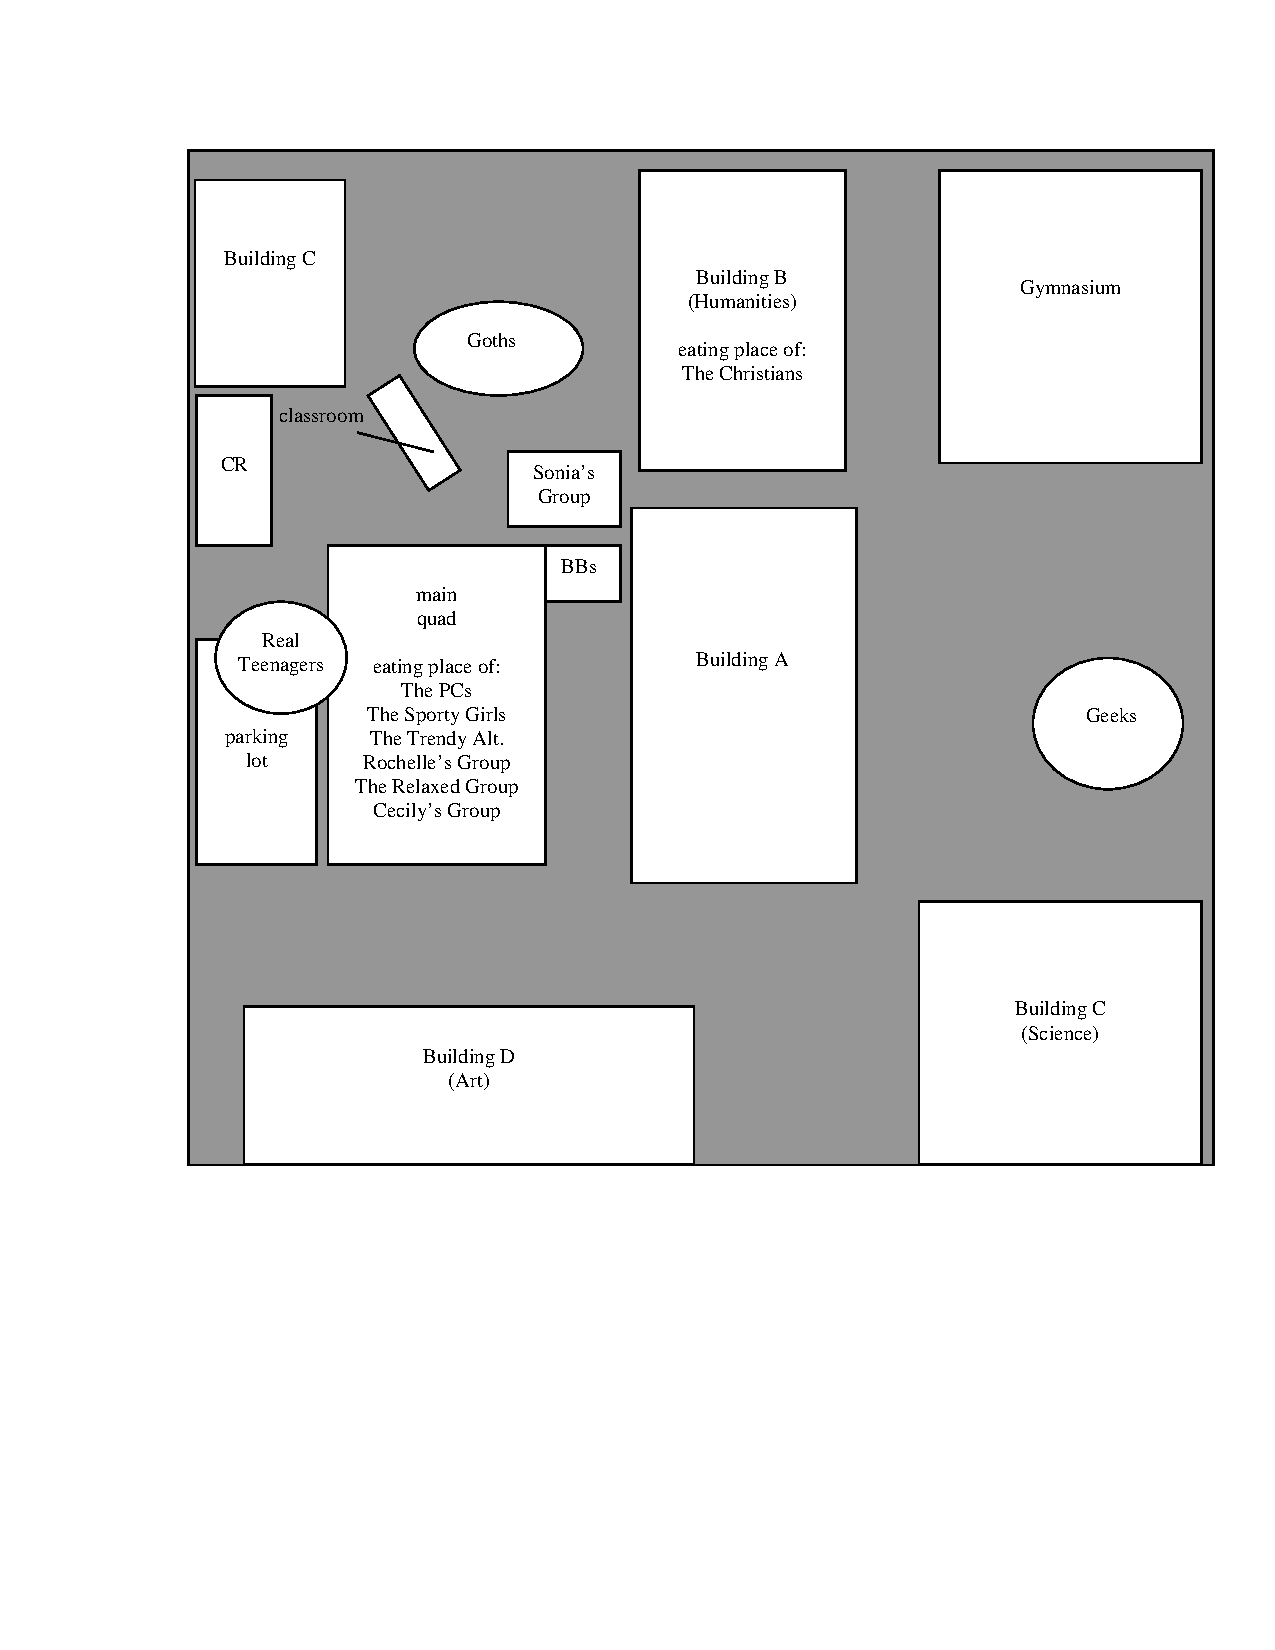
\includegraphics[width=\textwidth]{images/mySGHmap.pdf}
% 		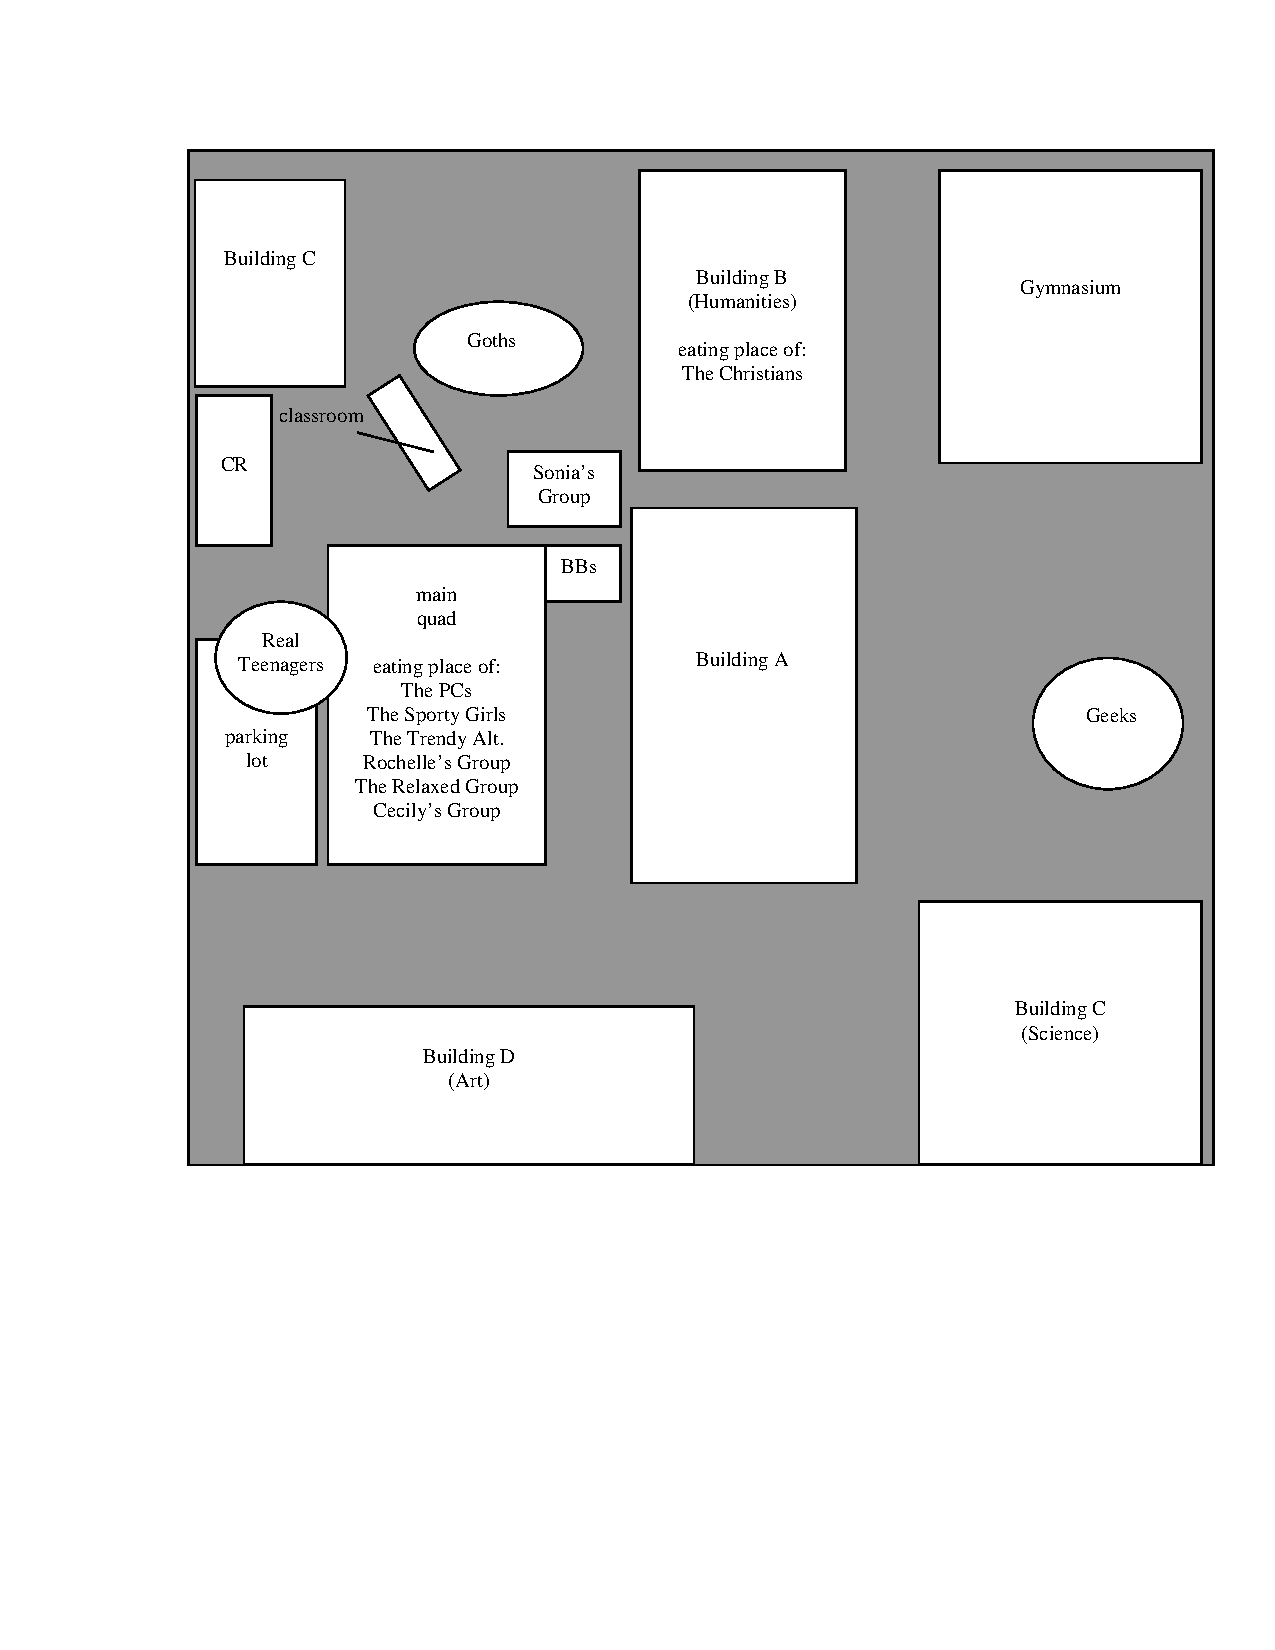
\includegraphics[height=.5\textheight]{images/mySGHmap.pdf}
	\caption{Map of SGH}
	\label{fig:mySGHmap}
\end{figure}


%Some of these group labels, for example \isi{The BBs}, were used by other girls to refer to only one of the sub-groups of a larger, merged group. However, for simplicity, I have adopted the terms to refer to the large, merged groups. 

\tabref{CRNCR} displays the division of the groups into the Common Room (CR) groups and the Non-Common Room (NCR) groups.\footnote{During the Study period, \isi{The Pasifika Group} often used the common room when no one else was there. However, they refrained from using the room when it was full of CR girls (e.g., during lunchtime) and they did not adopt the \isi{norms} of the CR girls. Therefore, these girls have been identified as \isi{NCR girls}.}  These groups will be discussed in more detail shortly.

     
     
\begin{table}[t]
\caption{Common Room (CR) and Non-Com\-mon Room (NCR) Groups, in the or\-der in which they are dis\-cussed}\label{CRNCR}
	 \begin{center}
		\begin{tabular}{ll}\lsptoprule
	
CR&NCR\\
	\\ \midrule
\isi{The PCs} & \isi{The Pasifika Group}\\
\isi{The Sporty Girls} & \isi{The Goths}\\
\isi{The BBs} & \isi{The Real Teenagers} \\
\isi{The Trendy Alternatives} & \isi{The Christians}\\
Relaxed Group & \isi{The Geeks} \\
Rochelle's Group & Cecily's Group\\
 &  Sonia's Group\\
 & Loners \\

\lspbottomrule
		\end{tabular}
	
	\end{center}
\end{table} 

\subsection{CR groups}
\label{group:CR}

The differences between CR groups were more subtle than those found between the \isi{NCR groups}. In general, girls in CR groups took part in school activities and played sport. They represented a mainstream P\=akeh\=a (New Zealand European) sense of style. Being prude or dressing differently than the other CR girls was not considered acceptable. They wanted to be liked and they wanted to be admired. CR girls conformed to each other in what they liked and what they did, thereby setting the \isi{norms} of the school. In some sense, they controlled, or at least embodied, the expectations of the school and of mainstream P\=akeh\=a society.

In the following sections, I describe the different groups who ate lunch in the CR. For a complete list of names of girls in each group, please refer to Appendix \ref{app:socialgroups}. Throughout the chapter, I refer to particular girls as the central/main member, a core member, or a fringe member. This is based on my observations of the groups and the information gleaned from conversations, such as which girls were named when describing both their own or another group. They were not labels used by the girls but are meant to give the reader an idea of the social make-up of each group.

\largerpage
\subsubsection{The PCs}
In addition to observing the groups, I asked the girls about what different groups there were at the school. When questioned, they almost always first mentioned \isi{The PCs}. The term ``PC'' refers to The Palms Crew, The Palms being a popular mall in Christchurch that the girls frequented. Girls from other groups admitted that they also sometimes shopped at The Palms, but the group had been labelled in junior years when \isi{The PCs} were the only group who hung out at the mall.

Non-PCs explained that in order to be a PC, a girl had to be good-looking. As an outsider to the school, it seemed less that \isi{The PCs} were inherently more beautiful than girls in other groups, and more that they wore the season's latest fashions from Christchurch's trendiest shops. While all PCs wore trendy clothes outside of school, only some members of \isi{The PCs} straightened their hair and wore make-up and trendy clothes to school. \isi{The PCs} who did not follow this trend went to the other extreme, wearing old track pants with holes and sometimes not brushing their hair. One of these girls, Kendra, explained that she didn't see the point of trying to look cute at school because there was no one she was trying to impress. Outside of school, however, she adopted the trendier styles of the other PCs. 

Talking with Glenda (\isi{The BBs}) and Ursula (a foreign exchange student who had joined \isi{The BBs}), it became clear that \isi{The PCs} were popular, not in the sense that they were the most liked, but in the sense that other girls looked up to them as the definers of what is and what is not fashionable. \isi{The PCs} were also sometimes referred to as The Plastics, a reference to characters in the Lindsey Lohan movie Mean Girls because they were known to be ``fake''\footnote{According to Urban Dictionary (urbandictionary.com), \textit{fake} is a term used to describe a person, usually a girl, who ``acts too nice to be real in order to lure in pathetic dopes and use/betray them, frequently crushing the victim's soul in the process.''  For more detail, see work by Stacy Lewis, who has conducted a linguistic analysis of ``mock fake'' speech: speakers imitating girls who are fake \citep{lewis2007}.} and to talk about each other behind each other's backs. When Ursula first came to SGH, she ate lunch with \isi{The PCs}, but she switched groups because she said their conversations made her feel uncomfortable. Both Glenda and Ursula were quick to add that, while as a group they did not particularly like \isi{The PCs}, each of \isi{The PCs} was nice on an individual level. I wondered whether this was related to the Losers Sit Alone rule: individual PCs being nice when interacting one-on-one because they did not want to be seen alone. Whether or not this is true, \isi{The PCs} were not the most well-liked group at SGH, but they were certainly the most popular.

%A number of \isi{The PCs} had jobs (several worked at the mall), and most of the central members of \isi{The PCs} lived in upper class suburbs and received money from their parents.

Neither Cleo nor Kim (\isi{The PCs}) were especially forthcoming with me and both eventually refused to take part in further interviews. Kendra, however, encouraged me to spend time with her group, explaining that I would get crazier stories from them than from any of the others. She was not entirely incorrect. Members of this group threw large, exclusive parties and they openly discussed sex, alcohol, and party pills. Noelle, June, and Joanna did fairly well in school, but the majority of \isi{The PCs} viewed school as a social arena rather than a learning centre. In fact, by the end of the year, Marilyn, Amber, Larissa, Kendra, and Minnie had dropped out. \isi{The PCs} who stayed until the end of the year expressed a mixture of excitement and sadness when graduating; they worried there would never come a time when everyone in their group was together again. As Tracy lamented, ``I think I need another year'' (Tracy, \isi{The PCs}, Interview, 22-10.)




\subsubsection{The Sporty Girls}
\isi{The Sporty Girls} were active in the school, though many of them had been more involved in previous years. Though distinct groups at the beginning of the year, contact between \isi{The PCs} and \isi{The Sporty Girls} increased as the year progressed. There were two groups within \isi{The Sporty Girls} who were especially close: Stella, Candice, Rachel, Elise, and Naomi; and Stella, Patricia, Ruby, and Betty. Stella is listed in both groups because she appeared to be the uniting member between them. Patricia's closest friends went to other schools, but at SGH her closest friends were Stella and Ruby. Kanani joined the group at the beginning of the year. She was the only girl in the study who switched from a NCR group to a CR group.\footnote{In terms of the production patterns that are presented in Chapter \ref{ch:prod}, Kanani behaved more similarly to the \isi{NCR girls} than the CR girls. Though I have not yet examined other features of her speech systematically, she appeared to use a mixture of phonetic features utilised by girls in both groups.}

Girls in the group viewed themselves as friendly, ``normal'', and ``in between''. The label, \textsl{Sporty}, was not something used by the girls in the group to refer to themselves. Though some of them wore athletic clothes to school, sports were not necessarily how they identified. In fact, Patricia did not play sport at all and, along with Betty and Ruby, wore some of the trendiest clothes of all the girls. \textit{Sporty} was a label used to refer to this group by girls in other groups, most likely as a result of the clothing worn by Candice, Stella, and Rachel. At the beginning of the year, Naomi also wore athletic clothes, but by the end of the year she had switched entirely to wearing trendy clothes and make-up.


\subsubsection{The BBs}
\sent{

Pam and Odette (\isi{The BBs}). Fieldnotes, 06-04.
\vspace{3 mm}

Pam:		the PCs may be cooler than us

Odette:	but we'll go further in life

}\label{ex:pamodette}

\vspace{5 mm}
 
\noindent Although girls in their final year at Selwyn Girls' High were no longer required to wear a uniform, some members of \isi{The BBs} continued to wear theirs, thereby acquiring the label ``the Blazer Brigade''. This was a friendly group of girls who were good students and who participated in a large number of school activities. At the beginning of the year there were two distinct groups, one of which was referred to as \isi{The BBs} and the other of which was referred to as Pam's group. Upon recognising that they were really very similar, they began to spend more time together and, by the end of the year, had merged into one group. I use the term ``BBs'' to refer to the ultimate, larger group. 

%[[Most of \isi{The BBs} are native speakers of \isi{NZE}. Glenda, however, spent her childhood in Australia and came with her family to NZ for \isi{high school}.

%Star, Madison, Pam, Natasha and several others were popular among the girls at Selwyn High, and in general, the group was well-liked. Priscilla, however, was not. CR and \isi{NCR girls} alike disapproved of her announcements of high marks on assignments, especially when her claims were proved untrue. Unfortunately, I had very little interaction with Priscilla as she was rarely free during study or breaks. When I commented on her busy schedule, she explained that she had many causes that kept her busy, and the school still expected her to do more. However, she continued to take part in causes she was less than enthusiastic about because if she didn't do it, who else would? ]]- REMOVE?  TMI?? 

Most BBs were friendly with girls from a number of groups, particularly those who also ate lunch in the common room. They were talkative in class and were involved in school activities. They went to parties and several of them were sexually active. They were more subdued than \isi{The PCs} in how they partied and they were less inclined to discuss details of parties with me. 

\isi{The BBs} viewed themselves as ``normal''. As shown in Example \ref{ex:pamodette} above and Example \ref{ex:notsupercool} below, \isi{The BBs} viewed themselves as somewhere in between the other groups. They were good students, but they did not view themselves as geeks.

\sent{
Andrea (\isi{The BBs}). Interview, 31-07.

\vspace{3 mm}

Andrea:   we're not like super cool \newline
					but we're not . like . super nerdy 
					
					[laughter]
					
					if that if that's that doesn't sound too mean

}\label{ex:notsupercool}

\vspace{5 mm}

They were school-oriented and felt a responsibility to be good role models for younger girls. They were friendly toward girls in other groups and Andrea claimed that they got along with other groups better than anyone else did. \isi{The BBs} who did not wear their uniform wore casual clothes, such as jeans and a t-shirt, and most of the girls planned to attend university. 


\subsubsection{The Trendy Alternatives}
\isi{The Trendy Alternatives} were artsy girls who took the latest trends and put a twist on them. The girls effectively treated Justine as the leader of the group and she was freely able (and willing) to interrupt the conversation and determine its direction.

Justine described university-bound students from other groups as ``the people that wanna do something with their lives'' (Justine, \isi{The Trendy Alternatives}, Interview, 03-05), but she did not feel the need to succumb to society's expectations of attending university directly after \isi{high school}. Though some girls in \isi{The Trendy Alternatives} were not particularly interested in school (e.g., Justine and Jewel), they planned to go to university after the age of twenty, at which point universities in New Zealand do not have entrance requirements. Other girls in this group were more school-orientated (e.g., Pascal) and went straight to university after \isi{high school}. 

\largerpage[-1] %longdi\isi{stance}
Although this group often ate lunch in the common room, they rarely spoke to girls from other groups. Kelly and Clementine were exceptions. Although they did not sit with other groups (and were therefore not viewed as traitors), they sometimes interacted briefly with \isi{The BBs}. Kelly was well-liked by girls in other groups. Lily, who expressed feeling like an outsider to her own group, was also friends with Rose (\isi{The Relaxed Group}) and Kanani (\isi{The Sporty Girls}), but she quickly left their side if someone from her own group walked into the room. Justine was on the committee that was planning the formal, as were a number of other CR girls. She had a clash with several girls from other groups over the venue for the formal. She was accused of being too outspoken on the subject and was reluctant to argue with them because she did not want to appear ``outspoken about being accused of being outspoken'' (Justine, \isi{The Trendy Alternatives}, Fieldnotes, 13-04).

%Other than Lily, this was a tight group who often met up together outside of school. On one occasion, they went to dinner at Tandoori Palace, an Indian restaurant in town, after which they split into two groups and tried to see how many times they could take the glass elevator in the Crowne Plaza. (In the end, only one group, who went up twice, was successful; the other group had a run-in with a security guard.)

\subsubsection{The Relaxed Group}\label{relaxedgroup}

Rose and Megan were the two central members of \isi{The Relaxed Group}.\footnote{Girls referred to this group as ``Rose's Group''.}  They were best friends and they had been since primary school. The group was also made up of Barbara, Katrina, Lorna, and Anita. Anita transfered to SGH at the beginning of the year. I met her just before the school's powhiri, a traditional M\=aori welcome ceremony which served to welcome new guests to the school grounds. She had just been approached by Rose and Megan, who, upon seeing me trying to figure out where I was meant to go, suggested that Anita and I stick together. Although shy and understandably confused by my role as a researcher rather than a student or teacher, Anita befriended me immediately. She also joined the group of the very first girls she met at the school. This was a group with whom I also felt comfortable and I often sought them out. Rose became one of the girls with whom I was closest and we have continued to stay in touch, nearly ten years since my first day at SGH.

While most of the girls in this group agreed that having fun was what life was all about, Katrina had a different outlook. She expressed frustration at being a teenager and she felt a great deal of pressure from her parents and the school, lessening her enjoyment of the life that her friends seemed to cherish. The other girls felt responsible to look after Katrina. This sense of responsibility was so strong that it tarnished the fun of the formal. Katrina did not want to attend, but her friends insisted that she come. She had a fight with her Mum just before the formal started and she spent the night distant and upset, sitting at the table with me rather than with her friends, and remaining there with my date when girls grabbed me to go dancing. Rose was emotional that night, worrying over Katrina. In general, Katrina was disappointed in Year 13, which she had been assured would be the best year of \isi{high school}. She was not impressed with \isi{high school} and felt ready for the next chapter of her life.\footnote{Katrina was much happier once she went to university. She has made good friends and she now admits that in \isi{high school} she would have liked to have been better friends with \isi{The Goths} but worried at the time that it would cause problems with girls in \isi{The Relaxed Group}.}  

%[it's kind of like there's \isi{youth culture} and then there's human beings [Katrina on being treated differently by adults - biancakatrinacandice18sept.trs]]  

When I asked Megan and Anita what made their group different from other groups, they explained that they were more relaxed and cared less about image than some of the other groups. They explained how they could wear jewellery or a belt if they wanted to feel cute one day but that they did not feel pressure to do so if they were not in the mood. Girls from this group wore little make-up to school and their style of clothing was the least trendy of all the girls who ate lunch in the CR. Barbara and Katrina played sport and Rose and Megan became increasingly interested in parties as the year progressed. Lorna was a fringe member and was also good friends with Rochelle's Group.

\subsubsection{Rochelle's Group}
At one point in the year I was struggling with my own personal relationship woes and girls in a variety of groups were exceptionally sensitive to my emotional state, for which I was (and continue to be) extremely grateful. One group in particular offered to listen and provide support because, as Camden explained, ``We know drama'' (Fieldnotes, 26-10). And indeed, these girls did. From break-ups to break-ins, these girls almost seemed to thrive on their struggles and the mutual fondness they gained through sharing their stories with each other.\footnote{Because of this drama, I have referred to this group elsewhere as the Drama Queens \citep{drager2008lsa}. I am not entirely happy with this label: It was not one used by any of the girls and they do not fit my stereotype of drama queens. Therefore, I felt it was misleading and have refrained from using the term here.}

This group was a CR group, but apart from Lorna's friendship with girls in \isi{The Relaxed Group}, they did not get along with CR girls from other groups. From my point of view, it seemed as though they intentionally instigated confrontations with other girls. Camden (Rochelle's Group) and Lily (\isi{The Trendy Alternatives}) openly talked badly about one another and Lorna (Relaxed Group/Rochelle's Group) rolled her eyes if one of \isi{The BBs} approached to ask her opinion on a Year 13 matter. Mindy, however, was quiet and friendly both in and outside of class and Rochelle made an effort to be friendly and to smooth things over with other groups. Perhaps it was she, the leader, who maintained their status as a CR group. She was the only one in her group who embodied the CR girls' trait of wanting to be liked and wanting to be admired.
 
Interestingly, these girls performed drama differently from other people I know. Rather than talking up their news as though it was full of juicy details, these girls downplayed their drama. My impression was that they wanted me to believe that they had so much drama in their lives that something that I might consider drama-worthy was hardly worth mentioning. For example, one day when I was talking with both Camden and Rochelle, Camden told me that she thought she was pregnant and that the father was neither nice to her nor wanted to be in a relationship with her.\footnote{She later found out that she was not pregnant.}  Rochelle, an incredible optimist on a number of occasions, stated with a sigh that she wanted to go ice skating and Camden agreed that ice skating would be fun. They were not avoiding the topic of pregnancy; both girls were quite open about sharing this type of information with me. The nonchalant manner in which the information had been provided and the quick change of subject to something entirely unrelated and, in my opinion, much less dramatic, left the impression that dramatic events were so commonplace in the lives of these girls that it hardly needed mentioning. That Camden explicitly made a claim on drama (``we know drama'') indicates that this was in fact the defining characteristic of this group and reflected how they viewed themselves.

%Other girls referred to this group as ``Rochelle's Group'' or sometimes ``Rochelle and Camden's Group''. , and the term ``Drama Queens'' is used because of Camden's claim on drama. Camden made this claim explicitly (``we know drama''), and she  Camden continually shared details of the drama in her life, both with her friends and with me. 

\largerpage
\subsubsection{CR groups as a constellation}
  
The CR girls' claim on the common room was no coincidence. The common room was a piece of prime real estate and they felt entitled to use it. Through actions such as writing on the whiteboard and posting photos of their friends on the wall, they not only used the room but made sure everyone knew that it was theirs. They believed, or at least claimed to believe, that everyone was friends with everyone else. If everyone was friends, there was no need to negotiate who was entitled to use a shared space like the common room.

Together, the groups who ate lunch in the common room formed a \isi{constellation of practices}, a term used by \citet{wenger1998} to refer to groups who were too broad and diverse to be considered communities of practice but who shared interconnected practices nonetheless. ``The term \textit{constellation} refers to a grouping of stellar objects that are seen as a configuration even though they may not be particularly close to one another, of the same kind, or of the same size'' \citep[127]{wenger1998}. He explains that constellations of practices are more abstract than communities of practice.  They need not be named nor do the individuals need to be aware that they form any kind of grouping. Though between CR groups there was a web of interconnected practices, they did not form the tightly woven bonds of a community of practice as described by Wenger. The CR girls were not the only \isi{constellation of practices} at the school. The whole of Year 13 was a \isi{constellation of practices} and, in fact, the whole of Selwyn Girls' High was as well. Constellations of practices can take a number of forms and can be observed at multiple levels of categorisation.

The CR girls also formed what I refer to as a \textit{constellation of stance}, an aggregate of individuals or groups of individuals who commonly take shared stances toward other individuals, concepts, and constructs. It is this that sets them apart within the constellation of the school. Here, I take \isi{stance} to mean ``a socially recognised disposition'' \citep[2]{ochs1990}. CR girls expressed similar views of themselves and similar attitudes toward these views (e.g., the view that they were ``normal'' and that ``normal'' was a positive attribute, that upward social mobility was a positive attribute and that people who did not aim for it were not going to go far in life). Through doing so, they form a constellation of \isi{stance} and they shared a number of interconnected practices (e.g., planning the formal, playing sport, and going to parties), thereby forming a \isi{constellation of practices}. The reason behind distinguishing between these different types of constellations will be clearer in the following section which discusses the \isi{NCR girls}: While the \isi{NCR girls} formed a constellation of \isi{stance}, they did not form a \isi{constellation of practices} that was separate from that which they also shared with the CR girls.

  

\subsection{NCR groups}
\largerpage[-1]
Despite the CR girls' claims, not everyone at SGH was friends with everyone else. There were girls who were not accepted into CR groups but who, for the most part, did not want to be. Though the groups shared little in common with one another, \isi{NCR groups} actively rejected the behavioural \isi{norms} set by the CR girls, and, in doing so, unwittingly shared a common \isi{stance}. 
 

Of course, the different \isi{NCR groups} each established their own sets of \isi{norms}. For example, girls in \isi{The Real Teenagers} were expected to party and girls in \isi{The Geeks} were expected to try hard in school. But the number of members in each of the groups was simply not high enough to overturn the school's \isi{norms} set by the CR girls. In other words, while there were \isi{norms} for each of the \isi{NCR groups}, they were not the \isi{norms} of the school.

\subsubsection{The Pasifika Group}

All members of \isi{The Pasifika Group} were M\=aori or Pacific Islander (PI).\footnote{Pacific Islander is a term used to refer to people with ancestry from Polynesia, Micronesia, and Melanesia. In New Zealand, it is does not usually include indigenous New Zealand M\=aori.} While there were M\=aori girls in other groups, ethnicity was not a topic they introduced into our conversations.\footnote{One exception was Kanani, who was proud of her Polynesian roots but distanced herself from \isi{The Pasifika Group} after switching to \isi{The Sporty Girls}. Girls in \isi{The Pasifika Group} were no longer friendly to her and she constructed her own sense of style (both linguistic and non-linguistic) that was reminiscent of both Pacific Island style and a style consonant with that of her new group.}  Girls in \isi{The Pasifika Group}, on the other hand, immediately identified themselves in terms of their ethnicity and expressed pride in their culture as well as frustration at the lack of ethnic diversity among the students and teachers at SGH and in Christchurch in general. They were particularly frustrated that the school did not seem to address their need for a more ethnically diverse faculty. There was no Pacific Island teacher and they felt misunderstood by the single M\=aori teacher at the school.  The school's failure to hire non-P\=akeh\=a teachers may well be due to a shortage of such teachers, but it left the girls feeling unsupported, as exemplified in Example \ref{ex:don'ttakeseriously}.
  
			
%Masina:  like for us brown people you know . PIs and Maoris . I mean they seem to lift I'm not being racist or anything . but you know they they just seem to lift like . other people . they believe they can do . better than us


\sent{
Masina, Alana and Lela (Pasifika Group). Interview, 20-09.

\vspace{3 mm}

Masina:  'cause I seen it happen quite a lot of times \newline
				but I mean a lot of parents have come in school . \newline
				um . to complain about it but they just .

Alana:  don't take . any notice of it

KD : really?

Lela : yeah it's ``oh yeah I don't care''

Masina: they don't take us seriously

}\label{ex:don'ttakeseriously}

\vspace{5 mm}

%[maybe this one isn't really needed and could be bad if someone at the school read it?]
%\sent{
%Marama:  		There's Miss [The only M\=aori teacher, name removed] 
	%					but she doesn't really know

%Lela : 			but . she doesn't really understand what . you know

%Masina: 		she's a beep [laughter] na honestly like 
		%				oh . she's nice and all but .

%Marama: 	na she's kind of a bitch
%}\caption{Marama, Masina, and Lela, Pasifika Group, 20-09}\label{ex:maoriteacher}

%\vspace{5 mm}

\noindent As demonstrated in Example \ref{ex:weneedsupport}, Masina and her friends felt as though they were treated differently, not by the other girls, but by the school itself. 

\sent{ 

Masina (Pasifika Group). Interview, 20-09.

\vspace{3 mm}
 
Masina:  but . yeah . um I mean they seem . \newline
					like they've had issues with . us brown people um .	\newline
					not attending school and stuff 		\newline
					and they just knock . all of us off . \newline
					like . all that like . one after one they h- \newline
					they're just like . completely give up on us \newline
					instead of giving us the support that we need to stay in school 
}\label{ex:weneedsupport}				
					
\vspace{5 mm}

\noindent They attributed the difference to the colour of their skin, explaining that most of their group had already left school and that they believed that teachers had ``written off'' those who remained. They also viewed themselves as different from the majority of girls, stating that they needed different kinds of support than other girls and wishing that there was a faculty member who understood where they were coming from culturally. They felt that while the school treated them differently, it did not treat them differently in a constructive way.


%Of the girls in \isi{The Pasifika Group}, I became most familiar with Marama, largely through attending her Textiles class, and it took some time before the other girls opened up to me. Once they realised that I was interested in them in addition to other groups in the school and that I would not tell their teachers and families about certain aspects of their lives, they began to share feelings of how they were treated differently from other girls at the school, not by the other girls but by the school itself. 

\isi{The Pasifika Group} had very little interaction with Year 13 girls from other groups. They did not eat lunch in the common room and they kept to themselves during class. One of their good friends, Ripeka, was very involved in the school, both with sport and with kapahaka (traditional M\=aori performing arts) and she had friends in other groups. Unfortunately, I was not able to record an interview with Ripeka.

Although girls in \isi{The Pasifika Group} had little interaction with girls from other groups in their year, they interacted regularly with more junior girls (who were also M\=aori or PI), which was not something done by girls in most other groups. 

\subsubsection{The Goths}

Only one member of \isi{The Goths}, Santra, wore black clothes and dyed her hair black, but girls in other groups referred to the entire group as \isi{The Goths}.\footnote{Goths are a youth subculture that see beauty in the dark side of life. They tend to wear black clothes, heavy eyeliner, and medieval-inspired clothing.}  All of the girls in this group described themselves as ``weird'' and they at least claimed not to care about what other people thought about them. They were intelligent girls who were enthusiastic students but who also questioned the school's ability to teach them life's most important lessons. They were knowledgeable about world events and had strong opinions about societal issues. Santra, Vanessa, Meredith, and Marissa were the original members of the group. In Year 12, \isi{The Goths} were joined by Tania (previously of \isi{The Relaxed Group}) and in Year 13, by Bianca, who seen less and less frequently with \isi{The Geeks} as the year progressed.

\isi{The Goths} had a particular area of the school grounds that they considered their own. It was separated by large plants from the courtyard where most of the other groups hung out and it contained a small wooden deck and a large rock. \isi{The Goths} ate there even when the weather was very cold and on rainy days they moved under the enclave of a building nearby. This group had eaten lunch in this area since the beginning of \isi{high school}. They were very territorial and girls from other groups rarely challenged their claim. However, there was one lunchtime where \isi{The Goths} had to assert their authority. They arrived to the area later than usual and some younger girls were sitting on the deck. Rather than approaching them and telling them to leave, \isi{The Goths} surrounded the deck and exclaimed in loud voices, ``Don't you hate it when people sit in their [sic] spot'' (Santra, \isi{The Goths}, Interview, 03-05). The younger girls gathered their things and left, glaring and mumbling in angry voices under their breath. Girls in \isi{The Goths} tended to be friendly, but the area where they ate was a part of how they constructed their \isi{identity}. They felt they had a claim on the place and they were willing to chance confrontation in order to preserve that claim.


\subsubsection{The Real Teenagers}

Some groups trusted me immediately. I was a researcher and university student. My presence had been approved by the school principal and this legitimised me in the eyes of some students (e.g., \isi{The BBs}). In contrast, it required more work to gain a \isi{rapport} with \isi{The Real Teenagers} and after over a month at the school, I began to lose hope that I ever would. One day, however, the opportunity arose.

``No entry''. The sign on the door was in clear view and it had not been there the day before. I did not know any way to the classroom other than through that door or through a maze of already-full classrooms. I had not seen Onya walk through the door, but I knew she had. Alex was walking toward it.\footnote{At the time, Alex and Onya were good friends. However, once Isabelle switched groups, Alex switched back to Cecily's Group, informing me that it was her ``real group'' while Onya stood listening nearby. Onya (\isi{The Real Teenagers}) and Cecily (Cecily's Group) did not get along though they had friends in common including Alex as well as others who did not go to SGH.}  She opened the door and moved aside the chairs meant to block the entrance, beckoning for me to follow. I hesitated a moment, unsure of whether I should follow this group of rather rebellious girls whose favour I had been attempting to gain (unsuccessfully), or follow my inclination to obey school authority. My desire to abide by the school rules was strong, perhaps a habitual remnant leftover from my own school days, or perhaps out of fear of losing the privilege of conducting research at SGH. The door, having been left unattended while I stood watching it, was just about to close, when suddenly I grabbed it and walked in. While I was maneuvering around the chairs that blocked my way into the hall, the teacher (whose class I had hoped to attend) emerged from her classroom. She glowered and reprimanded me. I felt ashamed and humiliated. Alex came to my defense, at which point the teacher began to aim some of the accusations at her. Alex and I both remained silent, neither of us informing the teacher who, besides myself, had walked through that door.

The shame I felt during the teacher's scolding surprised me. The reprimand itself was not what was surprising; I knew that I had disobeyed the rules and that I deserved to pay the consequences. I was surprised by my shame. 

But if shame was my payment, my reward was \isi{rapport}. From that day forward, this group of girls welcomed me to join them and they openly shared details of their personal lives to a level I had not anticipated. It was then that I appreciated the value of gaining \isi{rapport}, even when achieved through somewhat uncomfortable means, as exhibited by Geertz when he was finally able to gain \isi{rapport} with Balinese locals after siding with them during a government break-up of an illegal cockfight (Geertz 1973). Like Geertz, I had to face the temporary disfavour of an authority figure, but in turn I was able to gain the trust of those with whom I had previously had none. 

\nocite{geertz1973}

\isi{The Real Teenagers} were a group of rebellious girls who partied hard and, as they saw it, lived life to the fullest. One of the core members, Onya, gave an overview of their conversation topics: sex, drugs, and rock `n' roll. \isi{The Real Teenagers} claimed that they didn't care what others thought about them, but the explicit nature of the conversations and the volume at which they spoke while within listening di\isi{stance} of other girls suggested otherwise: They were out to shock. When in class two of \isi{The BBs} said that they wished their lives were as exciting as \isi{The Real Teenagers}', Alex and Onya laughed. They enjoyed their status as the crazy party girls and they were pleased when the other girls acknowledged it.

\largerpage
Most girls at SGH referred to this group as Onya's group; the ``Real Teenagers'' was not a name used by girls at the school. Toward the beginning of the year, Isabelle (formerly of \isi{The Goths}) decided to switch groups. Example \ref{ex:realrealteen} displays a conversation between Meredith, Vanessa (\isi{The Goths}) and me. 

\sent{
Meredith and Vanessa (\isi{The Goths}). Interview, 03-09.

\vspace{3 mm}

KD: how come Isabelle switched groups?

Meredith: to become a teenager

Vanessa: that was her words \newline
to become a teenager
 
KD: what's that mean?

Meredith: the group she's now with \newline
they go out and they get pissed like . every like . \newline
a couple times every weekend \newline
oh they just do stupid things

Vanessa: they have sex a lot

Meredith: yeah have sex a lot they just . \newline
they're like the real real real teenagers

}\label{ex:realrealteen}

\vspace{5 mm}

\noindent The central members of \isi{The Real Teenagers} were Onya, Claudia and Renee. Sarah was also a good friend, though she did not always get along with Onya. At the beginning of the year, Alex (Cecily's Group) and Onya spent a great deal of time together. However, Isabelle, rather than Alex, became Onya's close friend part-way through the year when Isabelle started dating Onya's good friend, Luke. Sally (Cecily's Group) became good friends with Renee over the course of the year but was rarely seen with the rest of \isi{The Real Teenagers}.

Though \isi{The Real Teenagers} and \isi{The PCs} shared a love for parties and a less than enthusiastic outlook toward academic subjects, the groups were different on a number of counts. \isi{The PCs} had values associated with more mainstream New Zealand society. Many of the girls belonged to higher socioeconomic groups and PCs who did not live in prestigious suburbs (e.g., Fendalton or Sumner) didn't talk freely about the area where they lived. \isi{The PCs} wore clothes from chain stores found at New Zealand malls. They wanted to be liked by girls in other groups and they smiled at girls who they talked badly about afterward. In contrast, \isi{The Real Teenagers} rejected mainstream values in favour of a more artistic chaos: homemade skirts accented in ribbons and lace, worn with Doc Marten boots, fishnet stockings, and handmade accessories from the clothing boutique where Claudia worked. Though high heels were not allowed at school, Onya loudly clomped down the main corridor wearing heels in defiance. Many of the girls belonged to lower socioeconomic groups. Onya talked with pride about living in Aranui, the poorest and most stigmatised suburb in Christchurch, and Renee explained that she had only brought a banana for lunch because her father couldn't afford the groceries that week (at which point her friends divvied up their lunches and shared them with her). They wanted other girls to recognise their party lifestyle and they wanted to be admired, but not for their money or their parents' social status. And they displayed no desire to be liked; they made it perfectly clear to all when there was someone they did not care for.

\subsubsection{The Christians}

In stark contrast to \isi{The Real Teenagers} were \isi{The Christians}. This group was made up of two girls: Esther and Theresa. Esther and Theresa felt most comfortable among people who shared their beliefs and adhered to their expectations of right and wrong. Despite their general satisfaction with life, they felt separated and different from the other girls at the school. Both worked hard at school and expressed enjoyment of their adolescent years.
 
Theresa, who was not religious prior to meeting Esther, grew up in a small rural town in New Zealand and Esther spent her childhood in a small village in France. They became good friends after Esther invited Theresa to Easter Camp, a multi-day Christian camp with live music, games, and activities. At the time, Esther had only lived in the country for a short time and had not realised that there were non-Christians in New Zealand. She invited Theresa assuming she would already be familiar with the idea of Easter Camp. Theresa came out of curiosity and had a wonderful time surrounded by more people than she had ever seen. Esther and Theresa were best friends from then on. 

Both Esther and Theresa dressed conservatively and said they would not feel comfortable wearing clothes, such as short skirts, that many of the other girls wore. Like girls in \isi{The Pasifika Group}, they interacted very little with other girls in their year but had several friends from youth group who were in more junior years. Exceptions in Year 13 were two of \isi{The Goths} with whom they occasionally interacted during Study, though only one of \isi{The Goths}, Marissa, encouraged the friendship. Both Esther and Theresa were good students and had conservative values and they both viewed Christianity as the defining feature of their group. There were other Christians at the school, but it was viewed as a characteristic of an individual as opposed to the central component of the group's \isi{identity}.
 
\subsubsection{The Geeks}\label{geeks}

The girls in this group did not fit my stereotype of ``geek'' at all. I viewed them as an eclectic group of individuals, each with their own distinct style. It was the most multi-national and multi-cultural group in Year 13. ``\isi{The Geeks}'' was a label used by other girls to refer to this group; it was not something used by the members themselves. Although this was not a group commonly mentioned by girls in other groups, CR girls used the term ``Geeks'' when asked explicitly about the group. 

The make-up of \isi{The Geeks}, most of whom were good students, only formed in Year 13. Joy, who was originally from Australia, attended another school in Christchurch before coming to SGH in Year 12. In intermediate school\footnote{Intermediate school is between primary and secondary school and is equivalent to junior high or middle school in countries such as the United States.}, Mariah had been in a group with some of \isi{The BBs}, but that group broke up when the unifying member moved to Australia. Valentina was new to SGH but quickly became a core member of the group. Aerial had a falling out with her former group (\isi{The Relaxed Group}) the previous year and \isi{The Geeks} befriended her. Bianca, a fringe member of \isi{The Geeks}, also spent time with \isi{The Goths}, and by the end of the school year was spending more time with \isi{The Goths} than with \isi{The Geeks}. 

On warm days, most girls at SGH ate lunch on the sunny side of the school. \isi{The Geeks}, however, ate lunch on the other side of the building from the main quad, as shown in the map in \figref{fig:mySGHmap}. The only other groups who ate in this area were in younger years. Joy and Mariah, the two central members, tended to dominate the lunchtime conversation. 

The styles worn by \isi{The Geeks} varied more than those worn by girls in other groups. For example, Aerial and Valentina wore short skirts and sandals, while Joy wore track-pants; Aluna and Nisha wore long flowing skirts, Kristin wore punk clothes with studded wrist bands, while Mariah wore corduroys and blouses from secondhand shops. Though styles of apparel varied among \isi{The Geeks}, girls from other groups saw fit to comment on their clothes, particularly those of Joy, Kristin, and Mariah. The other girls' expectations of what the girls in \isi{The Geeks} should wear were not the \isi{norms} of the school; \isi{The Geeks} were expected to dress differently from the other girls. For example, one day Mariah came to school wearing a purple nose ring. The other girls were shocked, telling Mariah that it didn't suit her. Megan (\isi{The Relaxed Group}), who was critical of Mariah's nose ring, had a lip ring herself and had commented on how she liked my nose piercing. It was not as though the girls did not accept piercings in general; they did not accept that Mariah, a Geek, would pierce her nose. After nearly an hour of taunting, Mariah removed her nose ring, revealing that the nose ring was one that did not require a piercing and that her nose was not, in fact, pierced. The other girls teased her even more after realising that the piercing wasn't real and Mariah never wore the purple nose ring to school again. 

%\footnote{I never heard anyone comment on clothes worn by Aerial or Valentina, despite their style being similar to that of \isi{The PCs}. A possible interpretation is that Aerial was once a CR girl, and it was acceptable for her to wear trendy clothing despite no longer being friends with the CR girls. Valentina, who was from South America, had a slightly different style, and the girls may have assumed and accepted that she dressed in a manner appropriate to where she was from.} 
%The geek girls resisted the comments for only a short time, eventually \isi{conforming} to the other girls' expectations of what they should wear. 
%By the end of the year, most of the girls had tried either beer or vodka at least once, but they did not party frequently. 

\subsubsection{Cecily's Group}

Cecily's Group was a group of friendly and funny girls. They had an alternative sense of style and liked live music and art. The majority of girls in Cecily's Group took art classes and several of them played musical instruments. Their interests were diverse and Sally explained how they each had their own little niche within the group through these different interests. Sally was an artist, Pania was a surfer, and Lindsey was a Christian, but they all enjoyed doing things together and valued each other's friendship.

When I asked Sally whether she thought the school was very divided, she first claimed that most people at the school got along but then added that there was some level of judgment by at least some people, as shown in Example \ref{ex:sallyjudges}.

\sent{
Sally (Cecily's Group). Interview, 11-04.

\vspace{3 mm}

Sally:	everyone just goes and has fun like

KD: yeah

Sally: 	I don't know . \newline
				but maybe slightly judgmental sometimes I don't know \newline
				there's some degree of judgment everywhere I suppose eh

}\label{ex:sallyjudges}

\noindent As discussed in Section, \ref{sec:salience}, the belief that everyone ``just goes and has fun'' is consistent with the \isi{stance} of the CR girls, whereas acknowledging that some girls are judgmental is consistent with the beliefs of the \isi{NCR girls}. This suggests that Sally's views were somewhere in between those of the CR girls and the \isi{NCR girls}.  In fact, the girls in Cecily's Group seemed to get along with girls in \isi{NCR groups}, such as \isi{The Real Teenagers}, as well as CR groups, like \isi{The BBs}. 

Members of Cecily's Group were good students, but they also partied and they genuinely seemed as though they didn't care to (or feel the need to) meet the social expectations of the CR girls. Cecily appeared to be the most central member and was usually the girl mentioned when other girls referred to this group. Because the girls in Cecily's group were very active at the school and had little free time, I had less of a chance to get to know them as well as I would have liked. 


%\subsubsection{Art Room girls}

%The Art Room girls formed a group of close friends who were active at the school. In many ways, they were similar to \isi{The BBs}, and in fact they were friendly with \isi{The BBs}. They wore alternative style clothing and were very involved in art class, so much so that they usually spent their breaks working on projects in the art room rather than sit outside with the other students.

%In contrast to the other \isi{NCR groups}, the Art Room girls were friends with a number of people in different CR groups. 


\subsubsection{Sonia's Group}

Sonia's Group was not a group that was pointed out by the other girls.\footnote{Sonia appeared to dominate conversations. Although I am not certain that she was actually the central member, I have used her name in the group's label.}  I came to know two of the girls in this group, Holly and Sonia, through attending their Study period. Though neither of the girls were seen conversing or sitting with \isi{The PCs} at school, Holly and Sonia saw some of \isi{The PCs} on a bus trip one weekend, a drunken night where groups are bussed between out-of-the-way pubs in and around Christchurch. Thereafter, both Holly and Sonia talked about \isi{The PCs} as though they were friends, leaving me with the impression that they looked up to \isi{The PCs}. Given their acceptance of the CR \isi{norms}, this group could potentially be classified as a CR group.\footnote{In the production analysis presented in Chapter \ref{ch:prod}, patterns in Holly's speech more closely resembled those found in the speech of the CR girls. However, I deemed it to be poor methodology to alter my qualitative analysis after this time,  but I interpret Holly's use of both linguistic and non-linguistic factors associated with CR girls to be consistent with her eagerness to conform to the CR girls' \isi{norms}. This is discussed further in \sectref{sec:idconstruction}.}  However, I have listed them here as a NCR group because they did not actually eat lunch in the common room.

\subsubsection{\isi{NCR groups} as a constellation}

The groups labelled here as NCR were a mix of diverse groups with very distinct ideologies and lifestyles. By placing them in a single group (NCR), I do not mean to imply that there were similarities among them. The trait they shared was a rejection of the practices that were established as normal by the common room girls, forming a constellation of \isi{stance}.	``We not only produce our identities through the practices we engage in, but we also define ourselves through practices we do not engage in'' \citep[164]{wenger1998}.

\largerpage
\noindent  The \isi{NCR groups} were separate, diverse groups with wildly different styles from one another, but crucially, they all viewed themselves as different from the other girls. 


\subsection{Outside of lunchtime}

The CR-NCR distinction extended beyond the lunch hour. There was one Study group in particular that exemplified the divide. While most groups in a single Study period were made up of fewer than 20 students, there was one period where over 30 students had Study. Due to the larger number of students, two classrooms (as opposed to the usual single room) were provided and the students were free to chose which of the two rooms they spent the period in. Without exception, girls in CR groups sat in one classroom and girls in \isi{NCR groups} sat in the other. The \isi{NCR girls} interacted minimally across the different groups, though occasionally Esther (\isi{The Christians}) commented on conversations between different members of \isi{The Goths}. The CR girls, on the other hand, sat on top of the desks and talked with one another throughout the Study period.

When running the \isi{perception} experiments, I asked the CR girls in this Study period if they would like to take part. Maya suggested that I ask the girls in the other room, commenting that they would be happy to help and that she would help later if I still needed participants.\footnote{Maya did later take part in the experiment.}  As I walked from one room to the other, I heard the CR girls laughing. I presumed that they were laughing at Maya's dismissal of my experiments, pawning the task off onto a group of girls with whom she did not care to interact. Alternatively, they may have been laughing because Maya told me what to do and I obeyed: I went to the ``others'', thereby acknowledging that they were the ``freaks and geeks'' who would take part in experiments and it was with them that I belonged. 

There was no label used to describe the differences between girls in one room and girls in another, but this is not surprising: Constellations of practices often go unnamed \citep[128]{wenger1998} and I suspect that constellations of \isi{stance} are even less likely to be named. Despite this, Maya had inadvertently acknowledged the divide between the Year 13 groups.



\section{Salience and stance}\label{sec:salience}
The \isi{Second Wave} of variationist studies emphasises the importance of using an ethnographic methodology in order to uncover social groupings of a community that are relevant to the speakers within that community. There is always a danger of a researcher imposing their expectations and prejudices upon speakers, thereby failing to identify categories that are relevant to the individuals being studied. However, I believe that less salient groupings of speakers can also be relevant to sociolinguistic variation. Extending the meaning to the context of SGH, I use the term \textit{relevance} to refer to how much a factor or group is ``connected with, or pertinent to the matter at hand'' (`Relevance' 2002), regardless of whether that factor or group is above or below the level of consciousness. I use the term \textit{salience} to refer to a gradient level of importance or prominence of an item in relation to its neighbours; the more salient an item, the more the item stands out. Salience attracts attention, and greater attention leads to a higher liklihood of \isi{awareness}.

\largerpage[-1]
Although girls at the school were acutely aware of the different, smaller groups (e.g., \isi{The PCs}, \isi{The BBs}, etc.), they were not aware of the constellations of \isi{stance}: the CR-NCR distinction. This is not to say that the girls were unaware of where other groups ate lunch (though several CR girls had trouble naming \isi{NCR groups}), but CR groups and \isi{NCR groups} were not listed as belonging to a shared grouping.  As mentioned earlier, Maya referred to the \isi{NCR girls} in the other room and treated them differently to the CR girls she was surrounded by, but this was the closest anyone came to acknowledging this divide. No one used labels to refer to CR versus \isi{NCR groups} and no one even mentioned the similarities across the different CR groups. The groupings ``CR girls'' and ``\isi{NCR girls}'' were not salient categories at the school and I want to make it clear that I am not arguing that they were explicit categories at all: They were groupings of girls who shared similar stances to the school's \isi{norms} of behaviour. CR girls shared the belief that they were ``normal'' and in doing so, they conformed to each other's \isi{norms}, thereby setting and perpetuating the \isi{norms} themselves. In contrast, girls labeled as ``\isi{NCR girls}'' shared a \isi{stance} that was something akin to different than the norm. They rebelled against the \isi{norms} of the CR girls in different ways (e.g., Santra of \isi{The Goths} wore all black; Esther and Theresa of \isi{The Christians} refrained from drinking alcohol; Joy and Aerial of \isi{The Geeks} sat at the front of the classroom; Marama and Angel of \isi{The Pasifika Group} did not reject their cultural values in favour of the P\=akeh\=a values that were embraced by the CR girls). These acts of defiance of the \isi{norms} served to construct their social personae. CR girls and \isi{NCR girls} formed two separate constellations of \isi{stance}. Consistent with work in the \isi{Third Wave}, I argue that linguistic variables can be indexed to stances rather than to any category of ``CR'' or ``NCR'', thereby allowing linguistic variables to be correlated with abstract groupings of individuals (constellations) of which the speakers themselves are less aware. A linguistic analysis and a discussion of how it correlates with these positions of ``normal'' and ``different'' can be found in Chapter \ref{ch:prod}. Here, I discuss some of the stylistic choices made by CR and \isi{NCR girls} and then I provide several examples of interactions with the girls that help to illustrate their different stances. 

A group's choice of lunch locale symbolises the position taken by those girls who conformed to expectations and \isi{norms} at the school and those who did not. The girls' choice of clothing, piercings, and activities supports this distinction. The CR girls most often wore clothes from chain shops found in malls throughout New Zealand. In most groups there was at least one girl with a facial piercing, usually a lower lip, eyebrow, nose, or Monroe (a piercing that is placed off-centre in the upper lip and resembles a beauty mark). Across the different \isi{NCR groups}, there was a much greater amount of variation in how they dressed. \isi{The Real Teenagers} mixed their own homemade creations with designer ones, and some had multiple facial piercings (e.g., both nostrils and the back of the neck). In contrast, \isi{The Christians} wore conservative clothing and had naked faces (i.e. no make-up or piercings). That girls from the different \isi{NCR groups} did not dress similarly to one another is not surprising. The girls were defined as \isi{NCR girls} not by what they were but by what they were not: CR. Instead of focusing on commonalities between them (of which there were few), I wish to highlight the multitude of identities and the manner in which they failed to conform to the behavioural \isi{norms} established by the CR girls. As individuals, they each rejected the expectations of the majority of girls at the school. Each of the groups rejected the \isi{norms} in different ways, but some of these acts, such as not eating lunch in the CR, were shared across the different groups. Therefore the common room was more than a mere eating place: It reflected the degree to which an individual conformed to the \isi{norms} established at the school.

%In fact, after the last assembly of the year at which I presented the idea of CR and \isi{NCR groups}, a number of girls, particularly CR girls, expressed surprise at the distinction. Is the CR-NCR distinction then a valid grouping, or is it a case of a researcher imposing categories on speakers that are not relevant to the speakers themselves?  I will argue that a grouping need not be completely above the level of consciousness for a particular speech community for it to be relevant for that community and for it to co-vary with linguistic variables.\footnote{Throughout this dissertation, I will use the term `relevance' to refer to importance of a factor that can be either above or below the level of consciousness, and the term `\isi{salience}' to refer to a gradient level of importance or standing out in relation to its neighbours; the more salient an item, the more conscious an individual is of the item. The categorical distinction of above or below the level of consciousness could be based on some threshold within the continuum of \isi{salience}.}  In Chapter \ref{ch:disc}, I will discuss how Exemplar Theory (see Chapter \ref{ch:litrev}), predicts that both phonetic variation and social variation can be below the level of consciousness and still be closely related.


%The girls could easily name who ate lunch where and with whom, but they did not consciously divide individuals into CR and \isi{NCR girls}. Girls were divided at the individual group level, not at the lunch locale level. Although this binary distinction between the groups is not a distinction that the girls were explicitly aware of, it reflects more than a mere eating place. CR girls established and conformed to the school's \isi{norms}, and \isi{NCR girls} walked to the beat of their own drum. 

%The girls who used the common room frequently expressed fond memories of their time at SGH. The memories were not necessarily of the school itself but of friends and amusing events. 

During interviews, CR girls most often commented on how everyone at SGH was friends and how there was not the clear division between groups that they associate with US high schools.\footnote{I suspect this was usually a comment made to me specifically as an American.}  For example, when I asked Rachel what groups there were at the school, she responded,

%Andrea (\isi{The BBs}) describes everyone in Year 13 as ``nice'', and 

\sent{
Rachel (\isi{The Sporty Girls}). Interview, 13-04.

\vspace{3 mm}

Rachel:	like there's . kind of like what everyone calls like \isi{The PCs} and then like \newline
				like little groups and stuff \newline
				but then in a way everyone I feel s- kind of gets on with everyone else as well \newline
				like I don't feel like it's that divided \newline
				well that's how I feel like some people might think it's different \newline
				but I kind of feel like I'm friends with everyone like like 

KD:	that's cool 

Rachel:	I don't feel like I don't have the right to t- go like \newline
		go up to a group and sit down with them \newline
		hang out with them one lunchtime \newline
		or anything like 
}\label{rachel-thatdivided}

\vspace{5 mm}

\noindent Rachel downplays any divisions among the Year 13 girls at SGH, going so far as to suggest that she could sit with another group at lunchtime. Though she made this claim, I only ever saw her sit with her own group and with \isi{The PCs} (a number of whom were friends with \isi{The Sporty Girls}) during lunch. 

%While Andrea (\isi{The BBs}) admits that there were groups in the past, she claimed that

When I asked Andrea (\isi{The BBs}) the same question, she explained that the groups were not as separated as they had been in previous years. She named the different groups in the following order: her own group (\isi{The BBs}), \isi{The PCs}, \isi{The Trendy Alternatives}, and Rochelle's Group, all of which were CR groups. Without being asked, Andrea explained why she had not named a single NCR group.

\sent{
Andrea (\isi{The BBs}). Interview, 31-07.

\vspace{3 mm}

Andrea: there's probably other groups \newline
that I don't really know about 

[laughing] 

. 'cause like . \newline
I probably really only know the groups \newline
that sit out on this . part of the lawn
}\label{ex:thispartoflawn}

\vspace{5 mm}

\noindent While there were several \isi{NCR groups} who ate within sight of \isi{The BBs}, Andrea did not mention them. Andrea only knew those groups that were highly visible at the school and those with whom her group shared a number of practices. She only knew (or, at least, only mentioned) the CR groups.

During a conversation in a Study period with both CR and \isi{NCR girls} present, Katrina, a CR girl, mentioned the tendency to downplay different groups even though they existed. Bianca, a NCR girl, added that she appreciated the diversity of groups at the school.

\sent{
Katrina, Barbara (\isi{The Relaxed Group}) and Bianca (\isi{The Geeks} and \isi{The Goths}). Interview, 18-09.

\vspace{3 mm}

Katrina:	but we kind of deny cliques as well

Bianca: yeah

Barbara: yeah

Barbara:	what did you call it? cliques?

Katrina:	yeah 

[laughter]
					
Katrina: 	that's what it is

Bianca: but I like variety 'cause it \newline
				I kinda do like variety in a \newline
				in like a school 'cause if you have everyone that looks the same \newline
				. you know it's kinda boring 
				
}\label{cliques}

\vspace{5 mm}

\noindent In contrast to other CR girls, Katrina acknowledged that there were divides at the school. Interestingly, Katrina was a CR girl who, in interviews conducted after her graduation, has admitted that she would have liked to have been better friends with \isi{NCR girls}.  Yet it took a NCR girl, Bianca, to state that she appreciated the diversity of personality types at SGH. That a CR girl did not make this statement is no surprise: \isi{NCR girls} valued being different whereas CR girls valued uniformity.

Though the CR girls did not state it explicitly, their claim on the only space set aside for their year reflects their status at the school. They were ``normal''. They were unified. The existence of cliques was denied. In a world where ``everyone'' got along, they saw no reason that they should not use the room. This tendency for CR girls to express feelings of unity is not to say that amiable relationships existed between all girls who ate lunch in the CR. In fact, there were a number of rifts between girls from different CR groups. However, disagreements tended to be between girls rather than against an entire group and many CR girls, when describing a group other than their own, mentioned one member of that group with whom they got along.

\largerpage[-1]
In contrast to the CR girls, \isi{NCR girls} consistently expressed how they felt different from other girls at the school, how they were not like everyone else. While CR girls viewed the social make-up of the school as a cohesive, unified community, \isi{NCR girls} felt separated from other girls at the school. In the exchange below, Esther (\isi{The Christians}), expressed how she felt that she had been labeled by the other girls as somehow different.

\sent{
Esther (\isi{The Christians}). Interview,  20-09.

\vspace{3 mm}

Esther:		I don't know how but I think I just like from Year 9 I just . \newline
					got the label that I wasn't . the same \newline
					I don't know like like it's weird 'cause

KD:	the the same as what?

Esther:	I li- as everyone else

}\label{ex:labelasdifferent}
  
\vspace{5 mm}
  
\noindent She attributed the difference between her and other girls at the school to her status as a Christian and in the statement above, she appeared to put the power of labeling in the hands of other girls. However, later in the interaction it became evident that the division was at least partially a result of her feeling that she couldn't relate to girls in other groups.

\sent{
Esther and Theresa (\isi{The Christians}). Interview, 20-09.

\vspace{3 mm}

Esther:  	I I think the difference is probably kah- 

[breathes in] 

we're both Christian

Theresa:  yeah 

Esther:		yeah \newline
					like it's kind of weird

Theresa:	it is quite weird

Esther:		yeah

KD:		what do you mean?

Esther:		like 'cause . we have different standards from everyone else \newline
					'cause yeah the . in history and they're all talking about \newline
					you know ``oh I slept	with so and so on	the weekend'' and and \newline
					and I mean I still wanna be their friend but it it's just kind of weird	'cause you know . \newline
					I don't . sleep with so and so on the weekend and yeah

}				

\vspace{5 mm}

\noindent Esther felt discomfort with some of the other girls' discussions. Rather than an external bias against Christians causing her di\isi{stance} from the other girls, her emotional response to the others' behaviour separated her from them. She would have liked to be friends with the other girls but it was hard to find common ground on which to connect. Wishing they could connect with the other girls is not to be confused with wishing they were more like the other girls: Both Theresa and Esther had a strong sense of \isi{identity} and were proud of who they were.

A very different group, \isi{The Goths}, also took pride in their differences and viewed them as a defining characteristic of their personalities. They, along with \isi{The Real Teenagers}, claimed that they did not care what others thought of them or whether others approved of them. As shown in Example \ref{ex:normalweird}, being ``normal'' was not necessarily considered a positive attribute by all girls. Whereas CR groups like \isi{The Relaxed Group} and \isi{The BBs} described themselves as normal, \isi{NCR girls} such as Vanessa and Isabelle did not want to have a claim on this label.

\sent{
Meredith, Vanessa (\isi{The Goths}) and Isabelle (\isi{The Real Teenagers}). Interview, 03-09.

\vspace{3 mm}

Meredith:	we're not weird we're normal everyone else is weird

\hspace{8mm} [pause]

Meredith:	I'm happy being weird

Isabelle:	well that's good

Vanessa:	as I said before if you don't like me then piss off

Meredith:	I'd hate to be normal it'd be so boring

Isabelle:	I know what is normal anyway?


}\label{ex:normalweird}

\vspace{5 mm}

\noindent Meredith began by claiming that she and the other Goths were not weird. She acknowledged that there was a difference between her and ``everyone else'', but that the difference was due to everyone else being weird, not her. When met by silence from her friends, she not only retracted her statement, but clarified that being weird was, in fact, a good thing. Isabelle, a Real Teenager, affirmed Meredith's claim on weirdness. \isi{The Goths} and \isi{The Real Teenagers} did not claim to be ``normal''. Instead they claimed to be ``weird'', setting themselves apart from the ``normal'' CR girls. 

The Pasifika girls also expressed feelings of difference. Marama and Lela agreed that they would prefer to attend a school with a higher percentage of M\=aori and Pacific Islander students. They were proud of who they were, but they did not feel like part of the school community. In Example \ref{ex:different}, their friend, Masina, stated what she viewed as the characteristic that set her apart from other girls: her skin colour. She explained that this had a negative effect on her opinion of the school.

\sent{
Masina, Pasifika Group, 20-09.

\vspace{3 mm}

			
			Masina: 		oh yeah I go to this school I'm so proud I go to this school \newline
			but . personally like to be honest I don't like this school  
			
			KD:	really why?
			
			Masina:	   	yeah . because like . well for a lot of reasons \newline
			I mean . like um . being a different . k- colour . you know . 

}\label{ex:different}

\vspace{5 mm}

\noindent The school was not ethnically diverse and girls in \isi{The Pasifika Group} felt that their culture and their skin colour made them different in the eyes of the school. Masina and her friends did not want to be like the other girls - they were rightfully proud of their culture and skin colour - but they would have liked it if there had been more students who shared these attributes. Each NCR group's view of how they were ``different'' was not the same, but they each established social identities that they viewed as different from the majority of girls at the school.

%While CR groups expressed feelings of unity, \isi{NCR girls} expressed feelings of difference. Across the different \isi{NCR groups}, the girls had very little in common. In fact, some of these groups like \isi{The Real Teenagers} and \isi{The Christians} were at opposite ends of the spectrum when it came to partying, boys and clothes. However, they formed a constellation of \isi{stance} because they shared a rejection of the \isi{norms} set by the CR girls. 

%  [MAYBE USE THIS ELSEWHERE - IN INTRO?  CONCLUSION?  LIT REV?]  It is not clear that communities of practice are always the best groups on which to focus for work in the \isi{Third Wave}. While they are certainly a good place to look for socially-meaningful variation, there are other groupings of speakers that should also be examined. As discussed in \sectref{sec:waves}, \citet{podesvaunderrev} chose to focus on the individual, and \citet{zhang2005} examined groups that shared styles and stances but that did not fall into the traditional notion of a community of practice. Consistent with the \isi{Third Wave}, the research presented in this thesis viewed a speaker's \isi{stance} as the central element that is indexed to socially-meaningful phonetic variation. While the traditional notion of a community of practice was observed across the distinct groups at the school (e.g., \isi{The Pasifika Group}), some of these groups shared practices and others a common \isi{stance}, forming a \isi{constellation of practices} and a constellation of \isi{stance}. In Chapter \ref{ch:prod} I will present how variation in \isi{/k/} realisation patterns with these more abstract groupings, providing evidence that linguistic variables can index an individual's \isi{stance}.

%Girls in the different CR groups shared much more in common, what they wore, where they partied, and how they partied. Of course, there were differences between the groups, but the differences were more subtle than those among the \isi{NCR groups}.
%and by a more mainstream P\=akeh\=a New Zealand culture.

%Even the Jocks and the Burnouts were not coherent groups but social networks \citep[11]{eckert2005}.


% [maybe add back in???] and the extent to which they rejected the expectations of what it \textit{means} to be a teenager.

%Further evidence that the CR-NCR distinction is relevant despite being below the level of consciousness is that it co-varies with linguistic variation observed at the school. As will be discussed in Chapter \ref{ch:prod}, acoustic analysis of tokens of the word \textit{like} produced by the girls reveals a significant relationship between \isi{/k/}-realisation, whether the token is quotative, and whether or not the girl is in a group who ate lunch in the common room. There are, of course, a myriad of differences in the phonetic realisations of other variables in the \isi{NCR girls}' speech. However, in addition to whether or not they eat lunch in the common room, the similar realisations of a phonetic variable among \isi{NCR girls} is a reflection of their rejection of the \isi{norms} of the school.

  


\section{A Bit of Self reflection}

I entered the school an outsider, but to what extent did I manage to get ``in'' with the different groups?  This varied depending on the group and the individual. In this section, I discuss my impressions of how well I knew different girls in different groups. An overview of the different groups and my \isi{perception} of how close I was with each of the girls is shown in Appendix \ref{app:socialgroups}.

\subsection{The BBs}
\isi{The BBs} immediately befriended me. Of all the girls, they reminded me most of my friends from \isi{high school} and as a result I was more comfortable around them than some of the other groups. Though I felt \isi{The BBs} were happy to be my friends, I did not have the feeling that they valued our relationship as much as some other girls seemed to. However, Jane claimed that she felt I was ``just kinda like another girl'' (Interview, 09-05), suggesting that perhaps from her point of view, I had been accepted.
%quote is from 9 may interview with Jane, about 1/4 through

During the second to last week of school, \isi{The BBs} invited me along to their champagne breakfast which was to be held on the morning of the last day of school. Pam approached me and asked if I would like to join them and when I said I would, I realised a number of \isi{The BBs} were watching to see how I would respond. They seemed pleased with my acceptance and they refused to take the money I tried to contribute. 

Several of the groups had planned to have real champagne on the morning of graduation, but the school was successful in their intimidation tactics and most groups abstained, including \isi{The BBs}, who had their breakfast near the front quad on school grounds. We drank sparkling juice in lieu of champagne and they brought a kiosk-like cooking trailer where they made eggs and sausages. But prior to the breakfast, we were met with a shock. In what the day before had been a perfectly green grassy quad covered in newly laid sod, there was a Christmas tree. It was not in a stand: It had been stuck into the ground so far that it could not be pulled out. The girls began to laugh, realising that it was a prank played by boys who I suspected were from an all boys' school nearby. The girls took photos with the tree and everyone commented on it while we ate. School officials arrived and, after some time, they were successful in removing the tree. Girls in other groups began to arrive and \isi{The BBs}, having been first on the scene, became the expert witnesses. The school questioned the girls (as well as me) on who had put the tree there.\footnote{The rumour was that the prank had cost the school upwards of \$10,000 because damage had been done to the recently installed sprinkler system.}  I did not know who had done it and the girls either did not know or did not tell; I thought it best if I did not ask.

That \isi{The BBs} invited me to their champagne breakfast and included me in their photos suggests that perhaps there was some element of truth to Jane's statement. While I would not claim to be ``just kinda like'' one of them, we had established a relationship that was mutually enjoyable.

\subsection{The Trendy Alternatives}
\largerpage
\isi{The Trendy Alternatives} were friendly and seemed curious about me, though I felt Justine and Jewel viewed me with some skepticism. Lily, Clementine, Christina, and Kelly were \isi{The Trendy Alternatives} who I felt closest with. Lily and I sent texts back and forth throughout the year and we went shopping and met for coffee even after she signed out of school.   

\subsection{The PCs}
A number of \isi{The PCs} wanted nothing to do with me or, at best, viewed me as a vehicle in promoting their status as the most interesting, popular, and beautiful girls at the school. When I first entered the school, they talked with me enthusiastically, but after several months they seemed to have lost interest, perhaps when they realised that I was talking with all of the groups, even those who were considered geeks. I was beginning to feel distraught that I would lose \isi{rapport} with them completely, but I also was not willing to give up my relationship with the other girls. I knew that without \isi{rapport}, none of them would be interested in completing the \isi{perception} experiment I planned to run. I hoped to collect responses from girls in as many groups as possible and, given their prominent status at the school, felt it particularly important that I included responses from \isi{The PCs}.

I was then given an opportunity to turn a negative aspect of my personal life into a positive factor for my research. I was leaving my husband. It was terrible. I was sad and ashamed and though all of the girls knew that I was married, I was reluctant to tell any of them about the separation for several weeks. Then one day I shared what I was going through. 

The first girls I told were some of the central members of \isi{The PCs} and one of their friends from \isi{The Sporty Girls}, a group who by this point in the year had combined with \isi{The PCs}. We were in Study and I was sitting with Tracy (\isi{The PCs}), Emma (\isi{The PCs}), Juliet (\isi{The PCs}), and Betty (\isi{The Sporty Girls}). It was one of the hottest days of the year and we had pulled the beanbags from the CR out into the sun. They were talking and I suppose I was even quieter than usual; I was certainly more distracted. They asked me about my husband. I was honest and told them I had left him. I was near tears and failed to hide the quiver in my voice. They consoled me and assured me that I had done the right thing, reminding me that we only live once and that we need to do everything we can to make sure that we are as happy as possible. Their response was mature and genuinely comforting. Though I had not intended it to be a \isi{rapport}-building conversation, such was the result. Through sharing my experience and feelings of pain and through their thoughtful comments and reassurances, we bonded. They began to invite me to record them more often and all four girls who had been present readily agreed to do the \isi{perception} experiment and even convinced several of their friends to do it as well. I believe they sensed that what I had told them was a difficult topic and that my emotion was real. Their view of me changed: Where previously I had been merely a tool for other means or a nuisance to avoid, what I had become was closer to a ``real'' person and a friend.

\subsection{The Real Teenagers}
Although initially I had been worried about not gaining \isi{rapport} with \isi{The Real Teenagers}, they ultimately became girls who I was very familiar with. Since graduation, I have received unsolicited emails from Isabelle, Alex, and Sarah; Onya approached me at a caf\'e after graduation, just to chat and introduce me to a non-SGH friend. During the course of the year, Alex gave a number of drawings to me. The one she gave me for my birthday is shown in \figref{fig:bdaydrawing}. In orange, green, and blue highlighter pen, it reads: ``To a very special varsity student... Have an ultra super funk (day after) Birthday... From the exceptionally awesome 7th form of SGH + Alex, cause shes cool, ancih.''


\begin{figure}
	\centering
		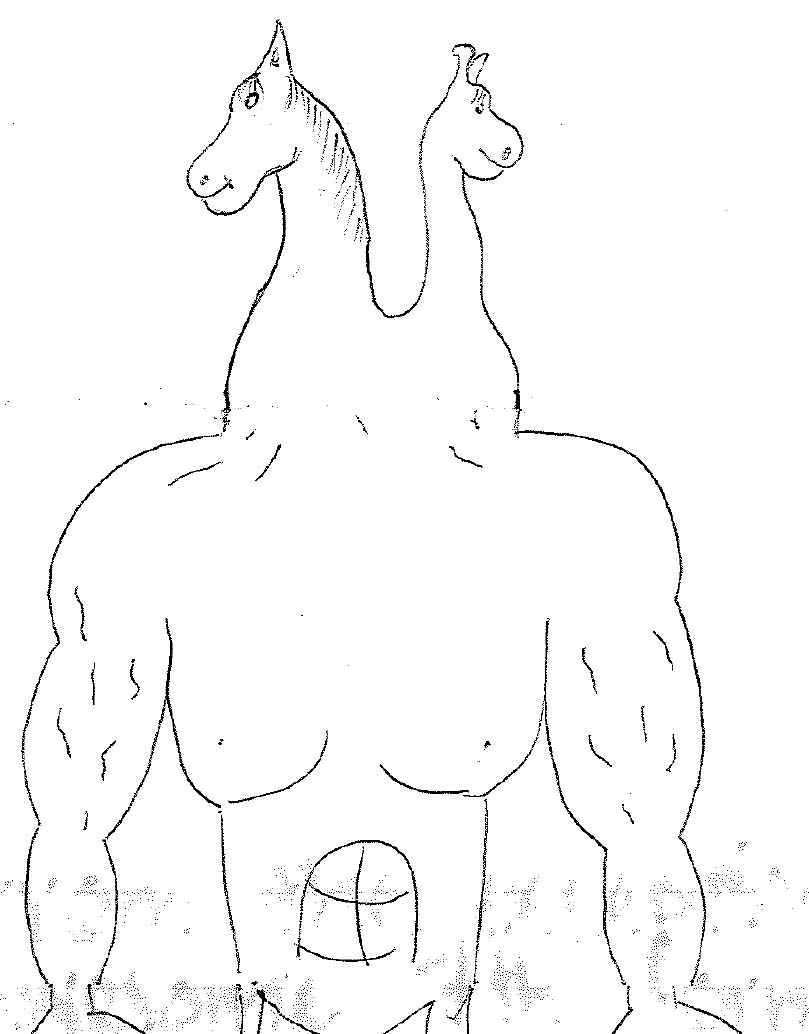
\includegraphics[height=3in]{images/bdaydrawingfromAlex.jpg}
	\caption{Drawing that Alex gave me the day after my birthday}
	\label{fig:bdaydrawing}
\end{figure}


\subsection{The Relaxed Group}
\isi{The Relaxed Group} was another group I came to know quite well. I was especially grateful for their presence on days when I was tired. I felt comfortable with them and accepted by them. Exchanges with them took less energy on my part. When I asked Megan and Anita if they would mind if I recorded them, they asked who I had already recorded. When I told them that I had already interviewed around 20 girls, they were shocked: Why wouldn't I ask them first?  They didn't seem as though their feelings were hurt; they simply seemed surprised that, given how close we were, they had not been among the first to be interviewed. Since graduation, I have met with Rose and Katrina and I am also still in contact with Megan.

\subsection{The Pasifika Group}
I became more and more familiar with \isi{The Pasifika Group} over time, especially with Marama. The girls in this group were especially interested in my California background: What was it like living near LA?  Are the boys better looking than here?  Have you ever met Snoop Dogg?  I enjoyed our conversations and it was my impression that they did, too. Although they were always friendly, I certainly never succeeded in feeling ``just like'' another girl in the group. They shared sensitive information with me, but they also adopted a more formal speaking register when addressing me directly. 

%At her friends' prompting, she showed me her latest design, a cute miniskirt that looked as though it could have been purchased from a shop.. , though they never invited me to join them outside of school grounds.

\subsection{The Goths}
\isi{The Goths} were very open with me from the beginning. They were talkative and they were quick to help shape my \isi{perception} of them. They invited me to join them during lunch or morning breaks and then would (in a friendly way) argue over who I would follow to class, explaining that I would learn more about life at SGH in one class over another. I felt as though I knew most of \isi{The Goths} very well.
 
\subsection{\isi{The Christians} and The Geeks} 
I am not Christian and I never once felt that Theresa and Esther needed me to be in order to interact with them or to be seen with them. In fact, they did not seem interested in whether or not I was Christian; they never asked and they always cheerfully accepted when I wanted to join them. Similarly, \isi{The Geeks} were always welcoming and I immediately felt accepted by them. 

\subsection{The Sporty Girls}
I came to know \isi{The Sporty Girls} early on. Though Naomi and Rachel were the first two I got to know, Kanani and I became the closest by the end of the year. I have met some of her family and we continue to stay in touch.

\subsection{Rochelle's Group}
I was very comfortable with Rochelle's Group and I believe they enjoyed my company as well. They asked me to come to parties and, of all the girls, they were the most persistent in insisting that I come to the formal. Part way through the year, they began to go to the school gym during lunch to work out instead of sitting in the CR or in their usual place on the lawn. I joined them in the gym on occasion, though I never had the proper clothes or shoes to join in on the workout. They continually invited me to parties and made sure that I never felt excluded from Year 13 events.

\subsection{Sonia's Group}
Of all of the groups presented here, I knew Sonia's group the least. I had the impression that they were not interested in me or what I was doing at the school. The phonetic analysis (Chapter \ref{ch:prod}) conducted on Holly's speech is based on a recording of a conversation between her and Sonia. I was in the room during the conversation, but I was not included in it. 

%   [maybe work this back in!!!! - already worked best bit in :) ]     With all of these different groups, I shifted my \isi{identity}. I felt compelled to behave in a way that they would like me, though there were boundaries. I did not join Emma (\isi{The PCs}), Megan (\isi{The Relaxed Group}), or Mariah (\isi{The Geeks}) in bad talking girls from other groups. My silence was often taken as ignorance of who the individual was, though there was an occasion where a racist comment from Onya prompted sidways glances at me from her friends and when met by silence (and a raised eyebrow) they told Onya not to say things like that. It was not always a conscious decision, but I was aware that I acted slightly differently with different groups.   Despite being one individual, my \isi{identity} was far from constant across the different groups. Does this affect my results?  And if so, how do I interpret them? 



\subsection{When research and friendship blend}

During the course of my work at SGH, there were several girls who were forced to deal with major life challenges such as eating disorders, pregnancy, miscarriage, and the death of parents and loved ones. To protect the individual girls, I will refrain from describing these in detail. Suffice it to say that the challenges faced by the girls of SGH were far from trivial and I found myself shifting between being a researcher and being a friend.

In conducting ethnography, the distinction between being a researcher and being a friend is sometimes blurred; in even a short amount of time, strong bonds can form \citep[79]{milroy1987}. Ethnographers become a part of the lives of the people they study, but some researchers may have qualms about getting too close to one's subjects: One does not want emotion to interfere with science. ``Without science, we lose our credibility. Without humanity, we lose our ability to understand others'' \citep[13]{agar1980}.

There were times when the girls tested the boundary between my roles as researcher and friend in places where I felt there should be one. For example, while walking to the supermarket one Study period with Renee, Alex, and Claudia (\isi{The Real Teenagers}), Alex commented that I could buy them alcohol, as none of them were yet 18. I could see her watching for my reaction and I treated it as a joke and laughed. That was not a boundary that I was willing to cross and, despite testing it, I do not believe that Alex expected that I would.

%And Onya invited me to Renee's birthday party. Given that several of the boys they were dating were roughly my age, I probably would not have 


There were other times when I dropped the \isi{identity} of researcher entirely and acted strictly as a friend, like the day that Sage collapsed. I had met Rose's sister, Sage, on a few different occasions, such as when she asked Rose to borrow lunch money. Sage was two years younger than Rose and seemed shy and sweet, but Rose worried about her. Sage's two best friends had decided that they would no longer be friends with her after ``borrowing'' a large sum of money. Soon thereafter, she was jumped and beaten up at a party. Then one day I witnessed something at the school and, embarrassingly, I did not respond as I should have. 

It was just before class began and I was talking with Maya (\isi{The BBs}) outside her classroom, which was one of many lined along the hall. Uniformed students stood in clumps talking, holding books and bags. A junior girl was pulling at her hair and I could see that she was trying to cover up a hickey. Out of the corner of my eye, I saw someone fall. I didn't see who it was and my view was obscured by three younger girls. I assumed it was someone messing around. Maya saw the fall, too, but kept talking, also assuming that it was some kind of joke. It wasn't. After what seemed like an eternity (but was probably more like ten seconds) I realised that the girl was not getting up. I pointed and asked if she was ok, at which point the girls blocking my view moved out of the way, though they kept staring at the girl on the floor. She was convulsing in what looked like an epileptic fit. I recognised her: It was Sage. A teacher saw her at the same time and rushed to her side. I told someone to get Rose. Someone else ran to fetch the school nurse. I stood waiting, watching Sage convulsing and wishing that I had acted sooner, wishing that I could do something. The bell rang and classes began, but there we were, separate from it all. Sage had stopped convulsing, but she remained on the floor. The teacher asked if she knew her name, if she knew the date. Sage did not answer and looked around blankly. 

\largerpage
When Rose arrived, she rushed to her sister's side. Rose talked to her softly and it looked as though Sage was answering. The nurse came in. She assured Rose that her sister would be fine and asked her to call their Mum. Rose and I went into a nearby classroom that was empty. She didn't want her sister to see her cry and didn't want her to know how worried she was. Rose called from my mobile phone, but her Mum didn't answer. Feeling scared and frustrated, she let her arms drop and threw her head back. I hugged her, assuring her that her sister would be fine. She cried and explained that her sister hadn't eaten and that the recent trauma combined with a lack of food may have caused her to faint. After several minutes, Rose began to calm down. She was able to reach her Mum and they went to the hospital for tests. 

I remained with Maya and the other girls in the hall, feeling vulnerable and helpless. I felt impressively insignificant. We were all in shock and felt uncertain of how to continue our day. I left school wondering what I could have done differently to help Sage sooner and wishing I had gone to the hospital with Rose. I wanted her to know that if she needed the support, I was there as a friend and not as the researcher who followed her and her friends around with a recorder. I texted her, asking how she was doing and asking whether Sage was ok. I got a text from Rose that night saying that Sage was fine and thanking me for helping. How had I helped?  I could have (and should have) done more, but all I did was give Rose a hug. 

I suspect that researchers in my field will come under fire if they get ``too close'' to the people they study because emotions could interfere with research-related judgments. But when faced with a crying girl who needs a friend, I will give her a hug if that's the best I can do at the time. Removing the human element from the methodology of ethnography is wrong and artificial.   How could I avoid being there for Rose as a friend?  And why would I want to avoid it?  She had shared her hardships and worries with me during the preceding months. Not only would it feel unnatural to dismiss our friendship on the basis of ``science'', it would be unethical.

%t's the human thing to do. I would go so far as to say that is unwilling to embrace the humanistic element of emotion in research is unfit to conduct this type of research. I genuinely liked the person she was. Furthermore, 

\subsection{Shaping interpretations}

How much were my interpretations of life at Selwyn Girls' High affected by my closeness with the girls, my own \isi{high school} experience, and my life prior to SGH in general?  Although I tried to go in open-minded, everyone's previous experiences inform the interpretations of new situations. \citet{mendozadenton2008} states explicitly that

\begin{quote}
	what I present as a text was filtered through my sensibility, my interpretation as well as my equivocation. Even what I noticed and considered as ``data points'' were selected in my \isi{perception} according to the sum of my prior experiences and my take on the situations encountered. \citep[44]{mendozadenton2008}
\end{quote}

\begin{quote}
	No ethnographer is a blank note\-pad just as no linguist is a tape re\-corder. \citep[48]{mendozadenton2008}
\end{quote}
 
\noindent It is the type of insight that would most easily be gleaned by an outsider who could view the entire situation (including me and my biases) from a different perspective. One effect of my personality that is obvious even to me is inherent in my interpretation of the incident with Rose's sister, Sage. The women in my family have a history of inheriting an irrational form of guilt from the women of the previous generation (which has the unfortunate effect of making the previous generation feel even more guilty). We take responsibility for the world's problems (e.g., children starving, greenhouse gases, the war in Iraq), not to mention problems in our personal lives, and feel guilty when we are unsuccessful in solving them. Sage's collapse was not my fault and many people would have responded the same way, yet I felt (and continue to feel) guilty that I did not do more to help. I recognise the lack of logic behind the guilt and I considered removing that aspect from the description of the incident from my dissertation and, later, this book. However, as it is, it is the honest portrayal of my interpretation of the situation. My inherited guilt combined with the close relationship that had developed between me and Rose served to shape how I viewed (and continue to view) what happened to her sister. I feel better acknowledging these effects and portraying my interpretation honestly rather than removing the emotions from the text. This way the reader can make up their own mind about how to interpret the situation without it being filtered through the reasoning of my self-conscious mind.

\begin{quote}
	On entering the community, an ethnographer carries more baggage than a tape recorder and a toothbrush, having grown up in a particular culture, acquiring many of its sometimes implicit assumptions about the nature of reality... The problem is not whether the ethnographer is biased; the problem is what kinds of biases exist - how do they enter into ethnographic work and how can their operation be documented. \citep[41-2]{agar1980}
\end{quote}

\noindent Interestingly, I also observed an influence in the opposite direction: I felt the memory of my own \isi{high school} life shift during my time at SGH. In the past, I had claimed that there were no cliques or ``popular girls'' where I went to \isi{high school}. After spending time at SGH, I realised that, like the CR girls, I had simply denied the reality of their existence. It took experiencing \isi{high school} life as an outsider for me to recognise and acknowledge this aspect of my own \isi{high school} life. This is not to say that my previous experiences did not help to shape my interpretations of the girls' socially constructed identities, but I was surprised to observe an effect in the opposite direction.

\section{Conclusion}

In sum, there were a number of groups at the school. The girls identified strongly with these groups and each girl found her own unique place within the group. Some of the groups (CR groups) valued conformity and viewed themselves as ``normal'' while other groups (\isi{NCR groups}) valued diversity and viewed themselves as different from the other girls. These aggregates of groups formed two distinct constellations of \isi{stance}. The following chapter investigates the degree to which phonetic variation at the school can be predicted by these different constellations. It also discusses the tendencies for particular girls to exhibit certain trends in the production of their speech and how these trends are consistent with non-linguistic expressions of their identities.


\newpage
\thispagestyle{empty}
\mbox{}
\chapter{\textit{Like}: Frequency and phonetic realisations}
\label{ch:prod}
\date{}
%\maketitle

\section{Methodology of interviews}\label{interview:method}

In a standard sociolinguistic interview, an interviewer asks questions designed to elicit the ``\isi{vernacular}'', which is essentially the range of speech styles used in informal situations when there is no interviewer present.\footnote{\textit{Vernacular} has been defined a number of different ways, including Labov's original definition of the term as ``the style in which the minimum attention is given to the monitoring of speech'' (Labov 1972: 208).  \citet{milroy1992} defines the term as ``real language in use''. I have put the term in quotation marks because I view speech styles as points along multidimensional continua and am dubious of the ability to identify and label some portion of these continua as the \isi{vernacular}.} Questions, such as whether the interviewee has ever had a near-death experience, are used to shift the focus from \textit{how} the narrative is said to the content of the narrative itself. Often followed by read passages and/or wordlists, the traditional Labovian style interview is a popular method to elicit speech, as it provides a means of lessening the effects of the Observer's Paradox. As speakers become more involved in the interaction, they become less focused on the fact that they are being recorded \citep{labov1972sociolingpatterns}. I adopted an alternative approach for my interviews at Selwyn Girls' High for the following reasons:\footnote{I use the word \textit{interview} to refer to a conversation that was recorded, even when it was not in a format traditionally used for interviews. This term is used to distinguish these conversations from interactions that were not recorded but were written in my fieldnotes.} 



\begin{enumerate}

\item[(1)] Previous work has shown that greater familiarity with an outsider decreases the amount a speaker will accommodate, thereby reducing the effect of the Observer's Paradox \citep{cukoravilabailey}. I did not begin recording until I had spent two months at the school, so I was already familiar with the girls at the time of the interviews.

\item[(2)] The Observer's Paradox was lessened even further through conducting multiple recorded interviews with many of the individual girls. They became more comfortable with the recording equipment after multiple encounters. 

\item[(3)] Speakers are less likely to accommodate to the speech of a researcher if family members or peers are present \citep[115]{labov1972principles}. Most of the interviews I conducted were with at least two girls.

\item[(4)] As a way of maintaining \isi{naturalness}, I gathered recordings of conversations between different girls rather than between me and them. In addition to preserving \isi{naturalness}, I used this technique because I was interested in documenting what they talked about with each other as opposed to what they talked about with me. 
\end{enumerate}

\noindent I conducted two different types of interviews depending on the situation. One involved multiple interviewees and spontaneous conversation between them and the other was an unstructured one-on-one interview. I will step through these in more detail shortly. In both types of interviews, girls asked what I was interested in and whether I had any findings thus far. I used these questions as an opportunity to ask about the social make-up of the school and how they viewed their own \isi{identity}. 

I most frequently used the first type of interview, which involved approaching girls who were already in conversation and asking if I could record them. Sometimes the place of conversation was too noisy for a quality recording and I suggested moving the conversation to a quieter room. After shifting rooms, the girls would continue the conversation where they left off, though they usually included me in the conversation for at least a part of the interview.  

This technique had drawbacks, as there were girls who I was interested in interviewing but who I had not seen interacting with a group small enough to be suitable for recording. With these girls, I conducted one-on-one interviews that involved questions and answers by both of us. As a result, the role I played in the conversations varied across the different types of interviews. While there were bound to be linguistic differences as a result of these different interview techniques, it did not significantly affect the sociophonetic analysis presented in \sectref{sec:phoneticlike}; individual girls who took part in the two interview types produced similar variants of \textit{like} across both.\footnote{The type of interview was tested statistically as a predictor for realisation in model 2, which is presented in \sectref{sec:phoneticlike}. It was not found to influence production on its own (p = 0.93), providing statistical evidence that the different token types were evenly distributed across the different interview types, nor was it found to be involved in an interaction with \isi{/k/} realisation (p = 0.33), providing evidence that the interaction between \isi{/k/} realisation and social group is not an artefact of interview type.} 
%Variation of other phonetic variables depending on the different interview types is an intended area of investigation for the future.

I had time on my side, so I invited all girls to ask me questions in addition to any I might ask. I did not want the interview to have an unbalanced distribution of power based on the interviewer-interviewee relationship and I chose instead to emphasise solidarity by highlighting our equality in the interactions. As a result, there are portions of some interviews where I talked extensively. Of course, this loose interview style would not suit researchers interested in eliciting the maximum amount of speech in the minimum amount of time. However, spending four days a week among the girls for an entire school year meant that I had enough contact time to use the most naturalistic context possible.

Recordings were made in various places on the school grounds (a classroom, the common room, or outside if it was sunny) using the AKG:C543BL table microphone  and a Marantz solid state recorder (PMD670), which records directly onto a CompactFlash digital memory card. 


\section{Variation in use of \textit{like}}\label{prod-like}


A select number of recorded interviews with the girls were transcribed using the tool Transcriber \citep{Transcriber-SpeechComm2000}, resulting in a transcribed corpus of over 15 hours of speech from 59 different girls.\footnote{Due to the sensitive nature of some interviews and the criteria set out by the Human Ethics Committee at the University of Canterbury, all recordings were transcribed by me.} 
\nocite{Transcriber-SpeechComm2000}

The analysis presented in this chapter focuses on the speech of 28 girls, 14 of whom were CR girls. All girls whose speech was analysed took part in the \isi{perception} experiments presented in Chapter \ref{ch:perc}.\footnote{I focused on transcribing interviews with girls who had participated in the experiments so that I could compare patterns of phonetic variables in their production to patterns of their responses during \isi{perception}.} Of the 42 girls who took part in the \isi{perception} experiment, the 14 CR and 14 \isi{NCR girls} who had the most speech recorded in the interviews were analysed. This was done in order to identify a large enough number of tokens for each speaker on which to conduct the statistical analysis.  The individual girls whose speech was analysed are shown in Appendix \ref{app:socialgroups}.  \tabref{tab:groupsprod} displays the number of girls from each of the individual subgroups whose speech was analysed.

\begin{table}[htbp]
\caption{The number of speakers in each subgroup that were analysed}	
	\label{tab:groupsprod}
	 \begin{center}
		\begin{tabular}{lrlr}
		\lsptoprule
		\sc cr group & \sc speakers & \sc ncr group & \sc speakers \\
 \midrule
\isi{The PCs} & 3       &Pasifika Group & 1  \\
Sporty Girls & 3  &\isi{The Goths} & 5 \\
Trendy Altern. & 3  &\isi{The Geeks} & 3  \\
Rochelle's Group & 1   &Real Teenagers & 2 \\
Relaxed Group & 3      &Christians & 2 \\
\isi{The BBs} & 1        &Sonia's Group & 1  \\\midrule
\sc total & 14  & & 14  \\

\lspbottomrule
		\end{tabular}
	
	\end{center}
\end{table} 


\noindent A great deal of variation can be found in the girls' speech. In the interest of investigating subtle differences in pronunciation across \isi{social groups} as well as across different meanings of a single word, this chapter focuses on variation within the word \textit{like}. The type of phonetic analysis that I conducted is time-consuming, particularly since I coded for a wide range of phonetic information. Given time constraints, it would not have been possible to examine these phonetic variables across a range of words without losing the theoretical insights gained from examining phonetic variation of lemmas that share an identical lexical form. These insights are discussed in \sectref{sec:proddisc}.

The word \textit{like} was chosen for analysis because several of the different meanings of \textit{like} were highly frequent in all of the girls' speech. This made it possible to conduct a within-speaker analysis of the realisations produced in spontaneous speech. Additionally, I hypothesised that socially-conditioned phonetic variation could arise depending on the nature of the different functions of \textit{like}: some of the functions are traditionally grammatical while others are discursive and are themselves layered with \isi{social meaning}. Given that they were highly salient at the school and were ideologically linked with \isi{youth culture} (and with certain individual girls at the school, in particular), \textit{like} seemed like a promising lexeme to focus on. I was particularly interested to see whether different individuals and groups of speakers produced different realisations that varied - not only according to their social group - but also depending on the token's grammatical function. For example, might there be a difference between groups in the pronunciation of a discourse-pragmatic function of \textit{like} (discussed below) that is not observed for the more grammatical functions (e.g., the lexical verb)? 

\largerpage
Furthermore, I am interested in the relationship between the phonetic realisation of a word and the word's probability of occurrence. I hypothesized that the likelihood that a speaker will producs a certain word might influence that speaker's pronunciation of the word. Focusing on the word \textit{like} allowed me to test this hypothesis (1) because I could control for word-internal phonological factors and (2) all of the girls produced tokens of \textit{like} though they did so to varying degrees.

Although this chapter focuses on phonetic variation in the word \textit{like}, there was a great deal of other phonetic variation in the recordings. This variation has not yet been analysed systematically. However, I intend to examine it in more depth in the future. 

For the analysis of \textit{like}, I used the different grammatical and discursive functions of \textit{like} as outlined by \citet{darcy2007}. Among its grammatical functions, \textit{like} may be a lexical verb (\ref{item:lexV}) or an adverb (\ref{item:adv}). These were the most frequent of the grammatical functions of \textit{like} found in the SGH data. Other grammatical functions of \textit{like} are the noun (\ref{item:noun}), the conjunction (\ref{item:conj}), and the suffix (\ref{item:suffix}). The examples listed here are from \citet{darcy2007}.


\sents{

\item  Lexical Verb:	I don't really LIKE her that much.\label{item:lexV} 

\item	Adverb:	It looks LIKE a snail; it just is a snail.\label{item:adv}

\item	Noun:	He grew up with the LIKES... of all great fighters.\label{item:noun}

\item  Conjunction: It felt LIKE everything had dropped away.\label{item:conj}

\item	Suffix:	I went (mumbling) or something like stroke-LIKE.\label{item:suffix}
\label{gramlikes}
}

\noindent The word \textit{like} also has discursive functions. It can serve as a discourse marker (\ref{item:dm}), a discourse particle (\ref{item:dp}), an approximative adverb (\ref{item:approxadv}), or a quotative (\ref{item:quote}). All of the discursive functions occur frequently in the speech of girls at SGH. The examples presented here are taken from interviews with the girls.

\sents{

\item  Discourse marker:	LIKE it real cracks me up. (Emma, \isi{The PCs}, 26-10)\label{item:dm}

\item  Discourse particle:	Lily was LIKE checking out my bro\-ther. (Ka\-na\-ni, The Spor\-ty Girls, 24-07)\label{item:dp}

\item  Approximative adverb: I did that in LIKE two days. (Theresa, \isi{The Christians}, 20-09)\label{item:approxadv}

\item Quotative:	and Mum's LIKE ``turn that stupid thing off.'' (Marama, \isi{The Pasifika Group}, 02-11)\label{item:quote}
\label{disclikes}
}

\noindent The lexical verb, adverb, quotative, and discourse particle were chosen for analysis because they were highly frequent, meaning that there were sufficient data for statistical analysis of their phonetic realisations. While the discourse marker is also highly frequent, it occurs at the beginning and end of phrases whereas the analysed functions of \textit{like} most often occur phrase-medially.\footnote{Included in the analysis were tokens of quotative \textit{like} where the remainder of the sentence was a gesture.}

Quotative \textit{like} can be used in a variety of different situations. For example, it can be used to report speech, thoughts, and gestures \citep{romainelange1991}. The analysis presented here combines all of the different pragmatic functions of quotative \textit{like} into a single category though it is possible that they could have different distributions or phonetic realisations.\footnote{An analysis of the different pragmatic functions of quotative \textit{like} revealed no function-based variation in these data, but this may be due to the relatively small number of tokens of each function.}



\subsection{Use of quotative \textit{like} at SGH}\label{section:uselike}



The frequency of use of the different types of \textit{like} varied depending on the individual. Based only on girls whose speech was analysed, two calculations were made with the aim of approximating a speaker's likelihood of using quotative \textit{like}. I decided to use two calculations because (a) frequency of use has been measured previously on the basis of both calculations and (b) I wanted to provide the most complete picture of the distribution of quotative \textit{like} among the girls.

The first measure of frequency of use of the quotative was the average number of times a token of quotative \textit{like} was produced for every hundred words produced by a speaker.\footnote{Word counts were generated automatically using O\isi{NZE} Miner. Words with hyphens (e.g., \textit{ex-boyfriend}) were counted as a single word.} A raw count of the quotative would not be representative of frequency of use due to differences in interview length across different girls. Though frequency of use is usually normalised per one thousand words, a smaller corpus necessitates normalising per one hundred \citep[264]{biberetal1998}. The measure is shown, by increasing use of quotative \textit{like}, in \tabref{tab:percentquote}. Token frequency measures are usually based on corpora, such as CELEX, that contain millions of words, but this is not realistic for examining speaker-specific frequencies. In the current study, the already relatively small word count of the corpus was made even smaller through examining intraspeaker frequency of use. Therefore, the values presented in \tabref{tab:percentquote} should be viewed with some caution.
 
  
  

  \begin{table}[htbp]
\caption{Values based on the first measure of frequency of use of quotative \textit{like}: The number of tokens of quotative \textit{like} per hundred words produced, ordered by increasing usage of quotative \textit{like}. Also shown is the number of all other quotatives by hundred words produced.}
  \label{tab:percentquote}
	 \begin{center}
		\begin{tabular}{lld{0}d{4}d{4}}
		\lsptoprule
\sc group & \sc cr/ncr &  \multicolumn{1}{c}{\sc total words} & \multicolumn{1}{c}{\sc quotative \textit{like}} & \multicolumn{1}{c}{\sc other quotatives} \\
		 \midrule

Patricia	& \sc cr &  4629	& 0.1080 & 0 \\
Santra	& \sc ncr & 6462	& 0.2786 & 0.2321 \\
Marissa	& \sc ncr & 1238	& 0.3231 & 0.1616 \\
Marama & \sc ncr & 	2783	& 0.3234 & 0.2515 \\
Mariah & \sc ncr & 	6126	& 0.3265 & 0.0490 \\
Juliet & \sc cr & 1032 &	0.3876 & 0.2907 \\
Christina	& \sc cr & 1440	& 0.4167 & 0.0694 \\
Tania	& \sc ncr & 3945 &	0.4309 &  0 \\
Katrina	& \sc cr & 1572 &	0.5089 & 0.0636 \\
Esther & \sc ncr &	4532	& 0.5296 &  0.0662 \\
Vanessa	& \sc ncr & 4728	& 0.5499 &  0.1904 \\
Justine	& \sc cr & 2022	& 0.5935 &  0 \\
Barbara	& \sc cr & 2867	& 0.6278 &  0.2442 \\
Bianca	& \sc ncr & 4197	& 0.6671 & 0.2144 \\
Clementine & \sc cr & 	3093	& 0.6790 &  0.1940 \\
Emma & \sc cr &	3916	& 0.7916 &  0.0255 \\
Jane	& \sc cr & 1236	& 0.8900 &  0.0809 \\
Theresa	& \sc ncr & 1279	& 1.0164 &  0.2346 \\
Sarah	& \sc ncr & 2150	& 1.1163 & 0.0465 \\
Rochelle & \sc cr &	1850	& 1.1351 & 0.1622 \\
Meredith	& \sc ncr & 6815	& 1.2032 & 0.1321 \\
Isabelle	& \sc ncr & 6776	& 1.5939 & 0.1476 \\
Betty	& \sc cr & 1040	& 1.6346 & 0.1923 \\
Tracy	& \sc cr & 1157	& 2.0743 & 0.1729 \\
Kanani & \sc cr	& 1769	& 2.0916 & 0.1696 \\
Rose & \sc cr &	3653	& 2.4090 & 0.1369 \\
Holly	& \sc ncr & 2878	& 3.1619 & 0.0695 \\
Joy & \sc ncr &	683	& 3.5139 & 0.1464 \\\midrule
   &               &  \textsc{total:~} 85868	& \textsc{mean:~} 1.0494 & \textsc{mean:~} 0.1337 \\

\lspbottomrule
		\end{tabular}
	
	\end{center}
\end{table} 

Also shown in \tabref{tab:percentquote} is the number of all other quotatives (i.e. quotatives that were not \textit{like}) per hundred words produced. When comparing the two normalised frequency measures, it is evident that while some speakers, such as Patricia, had low counts of quotative \textit{like} but produced few quotatives overall, other speakers, such as Santra, produced a large number of quotatives but used other quotatives nearly as much as they used quotative \textit{like}. 

The second measure was the percentage of all quotatives that were quotative \textit{like}, a calculation that follows the Principle of Accountability \citep{labov1972sociolingpatterns}. Because not all speech acts (and therefore not all recorded interviews) necessitate the use of quotatives, this measure provides a means of comparing the use of quotative \textit{like} across speakers within the context of other quotatives they might use instead; it is a reflection of how likely a speaker was to use quotative \textit{like} rather than one of the alternatives available. Therefore, it is a measure of \isi{token probability}, which is related to but also distinct from \isi{token frequency}.

\citegen{bybee2002} interpretation of the relationship between \isi{token frequency} and phonetic reduction depends on overall token counts. This means that in collecting counts of speaker-specific \isi{token frequency}, a researcher would need to record all interactions in which a speaker is involved over an extended period of time. Interpreting the measures of frequency presented here in terms of their reflection of speaker-specific \isi{token frequency} is problematic because (1) some speakers, in general, may be less likely to use reported speech than others, (2) some speakers, in general, may talk more than other speakers, and (3) the recordings may not be equally distributed across speakers for different types of speech acts. While the second measure can control for the latter of these concerns, it is less clear how to account for the first two. The first measure, however, does not control for any of these concerns. Therefore, the measures presented here are not analogous to \isi{token frequency}, but instead are informative of the relative frequency of a token. The first is the frequency relative to the number of words produced in the interaction and reflects the probability that, regardless of the speech act, a token will be quotative \textit{like}. The advantage of this measure is that not all girls may use the same amount of reported speech. However, this measure is problematic in that it assumes that the ratio of total speech to reported speech is equivalent to what would be observed across all interactions with the speakers, which is unlikely given the small number of interviews analysed. For this reason, this measure should be viewed with some caution. For the second measure, the frequencies are relative to the frequency of alternative quotatives that could be used. This reflects the probability that, if producing a quotative, the quotative will be \textit{like}. This measure of probability assumes that the ratio of quotative \textit{like} to the other quotatives used by a speaker reflects the ratio used by that speaker in interactions that were not recorded.

\nocite{bybee2002}



\newpage
\tabref{tab:percentlike} shows the percentage of all quotatives produced by a speaker that were quotative \textit{like}.\footnote{The null quotative (reported speech without the use of a quotative verb) is difficult to search for and was not included in the count. Though the null quotative can account for as much as 20\% of quotatives in other dialects, such as Canadian English \citep{tagliamontehudson1999}, during transcription it was noted that though the null quotative was observed, it was infrequent in the speech of the SGH girls. Furthermore, work in New Zealand has found low rates of the null quotative among females of a similar age to the girls in the current study \citep{buchstallerdarcy2009}.} Quotative \textit{like} was the most common quotative for all of these speakers, accounting for the majority of quotative tokens for all 28 girls. Nonetheless, there was some variation in its frequency of use. It was least frequent in the speech of Santra (Goths), Marama (Pasifika Group), and Juliet (PCs) and it was most frequent in the speech of Justine (Trendy Alternatives), Patricia (Sporty Girls), and Tania (Goths). This will be discussed further alongside discussion of the alternative quotatives sometimes used.



\begin{table}[p]
\caption{Values based on the second measure of frequency of use of quotative \textit{like}: The percentage of all quotatives produced by a speaker that were quotative \textit{like}, ordered by increasing usage of \textit{like}}
  \label{tab:percentlike}
	 \begin{center}
		\begin{tabular}{lld{0}d{2}}
		\lsptoprule
	
\multirow{2}{*}{\sc speaker} & \multirow{2}{*}{\sc cr/ncr} & \multicolumn{1}{p{2cm}}{\centering\sc total\newline quotatives} & \multicolumn{1}{p{2.5cm}}{\centering\sc \% quotative\newline \textit{like}}\\
  \midrule
Santra &	\sc ncr &	33	& 54.55 \\
Marama &	\sc ncr	& 16	& 56.25 \\
Juliet &	\sc cr	& 7	& 57.14 \\
Marissa	& \sc ncr	& 6	& 66.67 \\
Barbara	& \sc cr	& 25	& 72.00 \\
Vanessa	& \sc ncr	& 35	& 74.29 \\
Bianca	& \sc ncr	& 37	& 75.68 \\
Clementine	& \sc cr	& 27	& 77.78 \\
Theresa	& \sc ncr	& 16	& 81.25 \\
Christina	& \sc cr	& 7	& 85.71 \\
Mariah	& \sc ncr	& 23	& 86.96 \\
Rochelle	& \sc cr	& 24	& 87.50 \\
Esther	& \sc ncr	& 27	& 88.89 \\
Katrina	& \sc cr	& 9	& 88.89 \\
Betty	& \sc cr	& 19	& 89.47 \\
Meredith	& \sc ncr	& 91	& 90.11 \\
Isabelle	& \sc ncr	& 118	& 91.53 \\
Jane	& \sc cr	& 12	& 91.67 \\
Tracy	& \sc cr	& 26	& 92.31 \\
Kanani	& \sc cr	& 40	& 92.50 \\
Rose &	\sc cr	& 93	& 94.62 \\
Joy	& \sc ncr	& 25	& 96.00 \\
Sarah	& \sc ncr	& 25	& 96.00 \\
Emma &	\sc cr	& 32	& 96.88 \\
Holly	& \sc ncr	& 93	& 97.85 \\
Justine	& \sc cr	& 12	& 100 \\
Patricia	& \sc cr	& 5	& 100 \\
Tania	& \sc ncr	& 17	& 100 \\\midrule
& & \textsc{total:~} 900	& \textsc{average:~} 85.09 \\

\lspbottomrule
		\end{tabular}
	
	\end{center}
\end{table} 


The two measures for the \isi{speaker-specific frequency} of quotative \textit{like} are statistically correlated (Spearman's rho = 0.46; p$=$0.01). This is expected given that both measures are based on the number of tokens of quotative \textit{like} for each speaker. However, notice how for some speakers with a low number of overall quotatives (e.g., Patricia, Tania, and Justine) the two sets of values are very different in terms of how the girls are ranked in their respective frequencies of use. It is likely that this is a result of calculating the first measure over the relatively small amount of speech recorded for each speaker. This emphasises the importance of analysing quantitative data in terms of the context in which it is relevant when working with a small corpus. 

In both measures, CR girls produced more tokens of quotative \textit{like} than \isi{NCR girls}, as shown in the boxplots in \figref{fig:ComparingQLikeMeasures}. However, the difference between CR and \isi{NCR girls} was not significant for either measure (Wilcoxon, p = 0.25, p = 0.8). 

\begin{figure}[p]
	\centering
		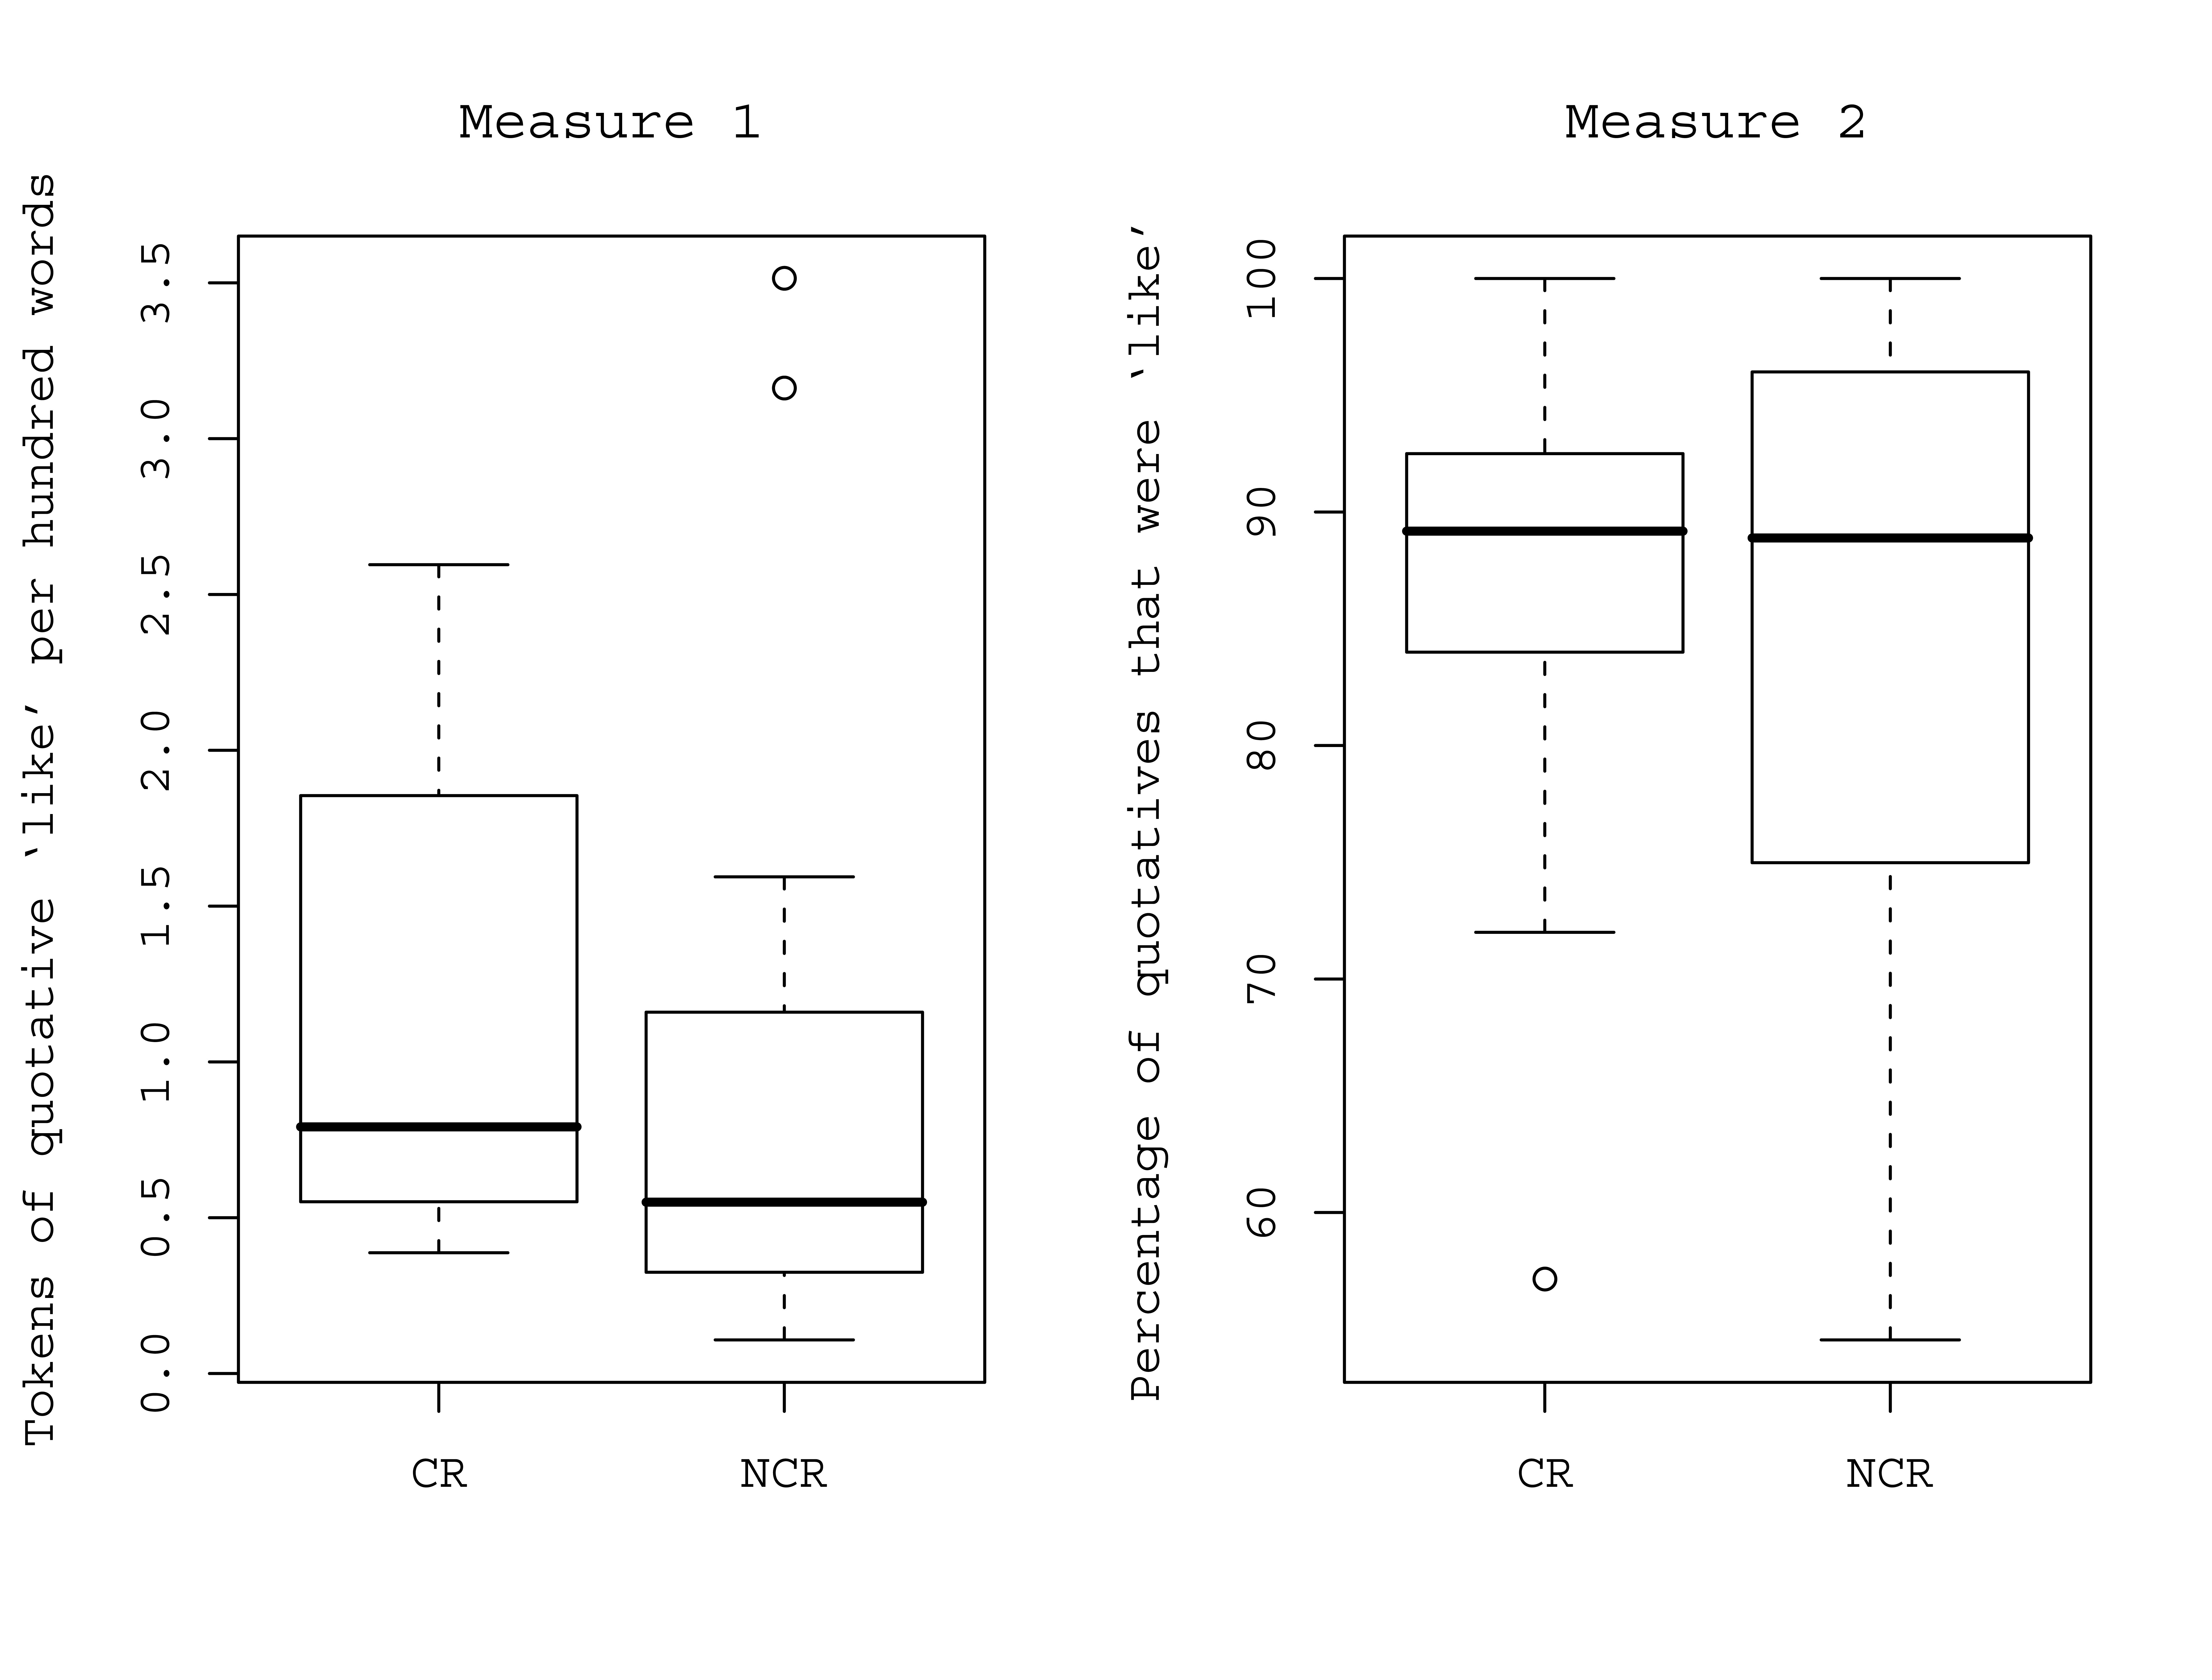
\includegraphics[height=.4\textheight]{images/ComparingQLikeMeasures.jpg}
	\caption{The frequency of use of quotative \textit{like} by CR and \isi{NCR girls}, based on the number of tokens per hundred words produced (Measure 1) and the percentage of all quotative that were \textit{like} (Measure 2)}
	\label{fig:ComparingQLikeMeasures}
\end{figure}

\tabref{tab:diffquotes} shows the percentage of all of the different quotatives used by CR and \isi{NCR girls}. The two tokens labelled as `other' were one token of quotative \textit{yell} produced by a Real Teenager and one token of quotative \textit{scream} produced by a Goth. 

\begin{table}[p]
\caption{The overall distribution of quotative verbs for CR and NCR groups}
  \label{tab:diffquotes}
	 \begin{center}
		\begin{tabular}{lrd{2}crd{2}}\lsptoprule
	
\multirow{2}{*}{\sc quotative} 		& \multicolumn{2}{c}{\sc cr} &	& \multicolumn{2}{c}{\sc ncr} \\
\cmidrule{2-3} \cmidrule{5-6}
              & n & $\%$ & & n & $\%$ \\
  \midrule

be like &  379 & 90.67 $\%$ &  & 488 & 86.83 $\%$ \\
say   &   28 & 6.70 $\%$  & & 44  & 7.83 $\%$ \\
be all  &  3 &  0.72 $\%$ & &  15 & 2.67 $\%$ \\
go    &    4 & 0.96 $\%$ &  & 10  & 1.78 $\%$ \\
think   &  4 & 0.96 $\%$ & & 3  & 0.53 $\%$ \\
other   &  0  & 0.00 $\%$  & & 2 & 0.36 $\%$ \\ \midrule
total   &  418 &   & & 562 & \\

\lspbottomrule
		\end{tabular}
	
	\end{center}
\end{table}

Quotative \textit{like} was the most frequent quotative in the speech of both CR and \isi{NCR girls}. CR girls used a slightly higher percentage of quotative \textit{like} than \isi{NCR girls}. The quotatives \textit{say}, \textit{be all}, and \textit{go} were more frequent in the speech of the \isi{NCR girls} than in the speech of the CR girls. With the low number of tokens, it is difficult to tell whether the differences between CR and \isi{NCR girls} is a result of more documented quotative tokens from the \isi{NCR girls} or whether it is something more socially meaningful. Though \textit{like} was still prevalent in their speech, it is possible that \isi{NCR girls} chose to use quotatives other than \textit{like} as an element in the construction of their identities. For example, Marama (Pasifika Group) was the speaker with the highest percentage of quotative \textit{go} (with 4 tokens) and though there were only two documented tokens of descriptive quotatives, \textit{scream} and \textit{yell}, both were produced by \isi{NCR girls}. In comparing the use of quotative \textit{be all}, only three CR girls, Clementine (\isi{The Trendy Alternatives}), Rose (\isi{The Relaxed Group}), and Rochelle (Rochelle's Group), used it once each whereas a greater number of \isi{NCR girls} used it and they used it more often: three tokens from Isabelle (\isi{The Real Teenagers}), two from Meredith (\isi{The Goths}), seven from Santra (\isi{The Goths}), and one each from Mariah (\isi{The Geeks}), Sarah (\isi{The Real Teenagers}), and Tania (\isi{The Goths}). Their use of alternative quotative verbs is consistent with their claims of being different from other girls at the school.

%There were also tokens of quotative \textit{go} produced by one of \isi{The Goths} and one of \isi{The Geeks}. The only documented tokens of quotative \textit{go} produced by CR girls were by members of \isi{The Relaxed Group}. The quotative \textit{be all} was found in the speech of \isi{The Real Teenagers}, \isi{The Geeks}, \isi{The Goths}, \isi{The Trendy Alternatives}, \isi{The Relaxed Group}, and the Drama Queens.  When PCs and BBs did not use \textit{like} they used \textit{think} or \textit{say}.  Likewise, when Holly (Sonia's Group), The Sporty Group, or \isi{The Christians} did not use \textit{like}, they used \textit{say}.  There were instances of all types used by \isi{The Goths}.  






\subsection{Use of discourse particle \textit{like} at SGH}\label{section:dplike}

There was also variation in how often the girls used discourse particle \textit{like}. A speaker's discourse particle frequency was calculated as the average number of tokens of the discourse particle produced by a speaker per hundred words of documented speech from that speaker. This is comparable to previous calculations based on tokens per thousand words that investigate how often people in different social categories (e.g., gender, age, and social class) use discursive functions of \textit{like} \citep[287-299]{anderson2001}. Ordered from most frequent to least frequent users, the values from the SGH data are shown in \tabref{tab:percentdp}. CR girls were significantly more likely to use the discourse particle than \isi{NCR girls} (Wilcoxon, p$=$0.01).\footnote{The frequencies presented here are considerably higher than those reported by Anderson from speakers of British English of a similar age (.0561 if re-normalised per hundred), and the difference would appear even greater if I had included token counts of all of the discursive functions as did Anderson.} 


\begin{table}[p]
\caption{Values of \isi{speaker-specific frequency} of discourse particle \textit{like}: The number of tokens of discourse particle \textit{like} per hundred words, ordered by increasing usage of discourse particle \textit{like}}
  \label{tab:percentdp}
	 \begin{center}
		\begin{tabular}{llrd{5}}\lsptoprule
	
speaker & CR/NCR & word count & \multicolumn{1}{r}{discourse particle}\\
  \midrule

Marissa	 & NCR &	1238	& 0.2423 \\
Esther	& NCR	& 4532	& 0.3089 \\
Santra	& NCR	& 6462 &	0.3405 \\
Vanessa	& NCR	& 4728	& 0.5500 \\
Marama &	NCR &	2783 &	0.5749 \\
Rochelle	& CR	& 1850	& 0.5946 \\
Sarah	& NCR	& 2150	& 0.6512 \\
Juliet &	CR &	1032 &	0.6783 \\
Isabelle	& NCR	& 6776 &	0.6789 \\
Holly	& NCR	& 2878 &	0.7992 \\
Joy	& NCR	& 683	& 0.8785 \\
Patricia	& CR	& 4629 &	0.9073 \\
Kanani	& CR	& 1769	& 0.9610 \\
Christina	& CR &	1440	& 1.0417 \\
Mariah	& NCR	& 6126 &	1.0774 \\
Katrina	& CR &	1572 &	1.1450 \\
Justine	& CR &	2022 &	1.2859 \\
Bianca	& NCR	& 4197	& 1.3581 \\
Barbara	& CR	& 2867	& 1.3959 \\
Betty	& CR	& 1040	& 1.4423 \\
Theresa	& NCR	& 1279 &	1.6419 \\
Jane	& CR	& 1236	& 1.7799 \\
Emma	& CR &	3916 &	1.8641\\
Tania	& NCR &	3945 &	1.9011 \\
Tracy	& CR &	1157 &	1.9015\\
Clementine	& CR	& 3093	& 2.1662 \\
Rose &	CR	& 3653 &	2.2174 \\
Meredith	& NCR	& 6815	& 2.6266 \\
\midrule
&& total: 85868 & \textnormal{\upshape mean:~} 1.1789 \\

\lspbottomrule
		\end{tabular}
	
	\end{center}
\end{table} 

\largerpage
There is a loose correlation between the number of tokens of discourse particle \textit{like} and the number of tokens of quotative \textit{like} per hundred words produced (Spearman's rho = 0.38; p$<$0.05). This relationship is shown in \figref{fig:ComparingQDP}. For speakers with less than one token of quotative \textit{like} per hundred words, there is a linear relationship between the frequency of use of quotative and discourse particle \textit{like}. This is not the case for the speakers with a greater number of tokens of the quotative per hundred words produced. Though it would be desirable to calculate an alternative measure of discourse particle frequency based on contexts in which it could be used (such as that conducted by \citealt{darcy2005}), it is not possible here given time constraints. 

\clearpage
\begin{figure} 
	\centering
		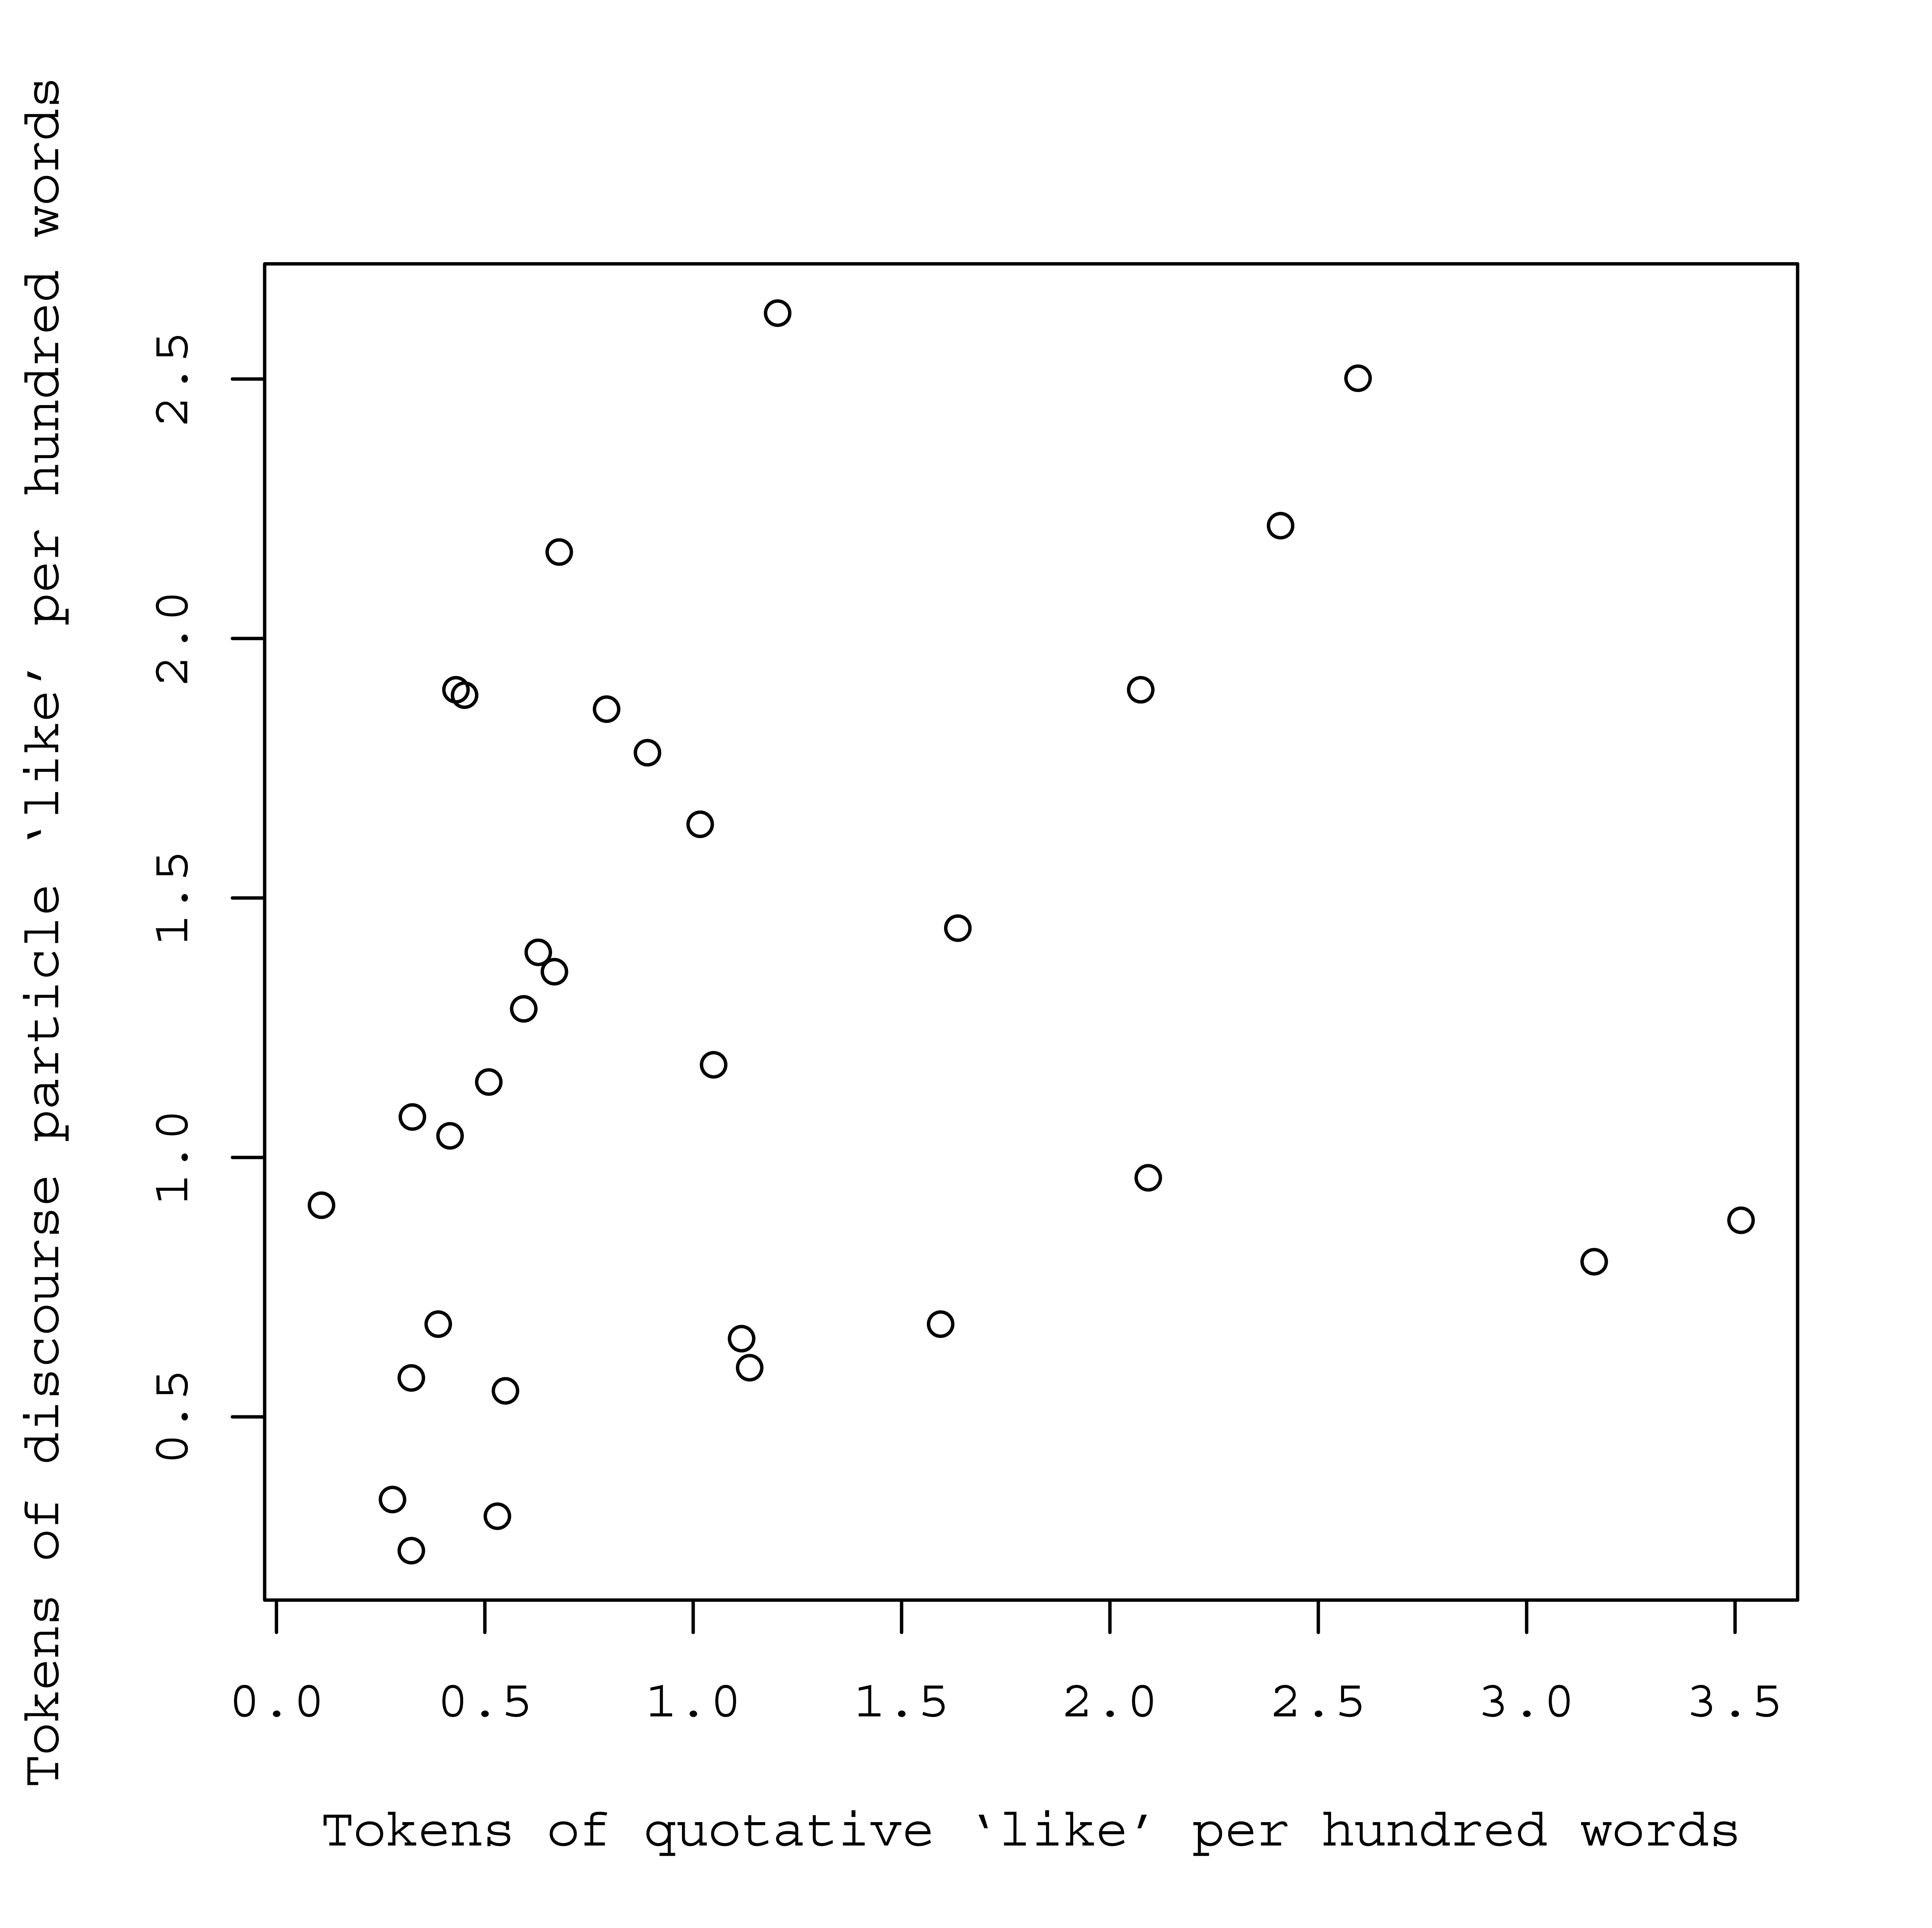
\includegraphics[height=.5\textheight]{images/freofuseCompare.jpg}
	\caption{Plot of the number of tokens of quotative \textit{like} and the number of tokens of discourse particle \textit{like} per hundred words produced}
	\label{fig:ComparingQDP}
\end{figure}


%%%%%%%%%%%%%%%%%%%%%%%%%%%%%%

\section{Phonetic variation of \textit{like}}\label{sec:phoneticlike}

There is variation among the girls' realizations of \textit{like} in several respects: whether or not the \isi{/k/} is realised, the length and quality of the \isi{/l/}, how diphthongal the vowel is, the vowel quality of the nucleus and offglide targets, the duration of the vowel, and the degree of \isi{glottalisation}. All of these factors were analysed in order to determine whether there was any fine-grained phonetic variation that patterned systematically with (a) whether or not a speaker was a CR girl and (b) the different functions of \textit{like}. 


The CR-NCR distinction at SGH was noticed prior to beginning acoustic phonetic analysis. However, in order to determine whether this was an appropriate social distinction to include in the statistical analysis, I conducted a classification and regression tree (CART) analysis (see e.g., \citealt{breimanetal1984}) predicting \isi{/k/} realisation before fitting the statistical model presented in \sectref{sec:prodresults}. Individuals grouped according to whether or not they ate lunch in the CR, which suggested that the CR-NCR distinction was in fact an appropriate social category to include in the model. \nocite{breimanetal1984}



\subsection{Methodology for acoustic phonetic analysis}\label{sec:phoneticmethod}


The various utterances of \textit{like} from the interviews were extracted automatically from the corpus using ONZEMiner \citep{onzeminer}. Because of the particular functions chosen for analysis, the vast majority of tokens did not occur at phrase boundaries, did not carry primary \isi{stress}, and were not the least stressed words in the sentence; only one token analysed occurred sentence-finally and carried primary \isi{stress}. 

I aimed to conduct acoustic analysis on 30 tokens of \textit{like} for each girl. Whenever possible, these 30 tokens were made up of 10 tokens of quotative \textit{like}, 10 tokens of the discourse particle, and 10 grammatical tokens. The grammatical tokens were made up of a combination of lexical verbs and adverbs depending on what was present in the data.\footnote{Preliminary analysis provided evidence that the lexical verb and the adverb were phonetically similar to one another for a given speaker in terms of \isi{/k/} presence and the degree of diphthongisation.} This, however, proved impossible for all girls due to low token numbers, and fewer than 30 tokens were analysed for some girls. For girls with more than 10 tokens of a particular function of \textit{like}, the first 10 tokens extracted were analysed provided that they were unobscured by background noise. The token distribution is shown in \tabref{tab:tokensanalysed}.

 
%summary(noapproxtype.lab)
 %        approxadv        dm        dp   lexverb      prep     quote 
  %      0         0         0       292       104       100       239 
%> summary(CRtype.lab)
 %         approxadv        dm        dp   lexverb      prep     quote 
  %      0        22        58       160        48        49      119  
%> summary(NCRtype.lab)
 %         approxadv        dm        dp   lexverb      prep     quote 
  %      0        11        29       132        56        51       120 
      %  summary(noapprox$CR)
     %CR NCR 
  %0 376 359 
        
\begin{table}[t]
\caption{The distribution of analysed tokens of \textit{like} for CR and NCR groups}
  \label{tab:tokensanalysed}
	 \begin{center}
		\begin{tabular}{lrrr}\lsptoprule
	
		& \sc cr 	&	 \sc ncr & \sc total \\
              
  \midrule
  
quotative & 119 & 120 & 239 \\
discourse particle & 160 & 132 & 292 \\
grammatical (lexical verb) & 48 & 56 & 104\\
grammatical (adverb) & 49  & 51 & 100 \\
grammatical (total) & 97 & 107 & 204 \\
total analysed      & 376 & 359 & 735 \\

\lspbottomrule
		\end{tabular}
	
	\end{center}
\end{table}

\newpage
The final dataset included 104 tokens of the lexical verb and 100 tokens of the adverb, resulting in 204 tokens of traditionally grammatical functions. There were 239 tokens of the quotative and 292 tokens of the discourse particle in the final dataset. Of the 3159 tokens of \textit{like} initially extracted for the speakers analysed, 735 tokens (or roughly	23\% of the tokens extracted) were analysed using detailed acoustic analysis.\footnote{The percentage of tokens extracted that were analysed breaks down by function as follows: 30\% of quotative \textit{like} tokens extracted, 28\% of discourse particle tokens extracted, 60\% of lexical verb tokens extracted, 40\% of adverb tokens extracted. If a greater number of tokens were analysed, it is possible that a larger number of factors would reach significance in an interaction with the social factor tested.} Tokens masked by noise or made ambiguous from false starts were not included in the analysis. 

The unequal distribution and the low token numbers for some groups would pose a problem for an analysis of the smaller sub-groups (e.g., \isi{The Goths}, \isi{The PCs}). The analysis presented here focuses on differences at the CR/NCR level, though individual speaker differences are discussed in \sectref{theindividual}.  
%They were then assigned one of the categories (discourse particle, quotative, or grammatical) based on the grammatical function of the token. 

Phonetic features of the tokens were la\-belled in Praat text\-grids \citep{boersmaweenink} in a way that allowed the analysis to be conducted both on gradient and discrete measures.\footnote{A small subset of the data was checked for consistency by an independent phonetician.} The bound\-aries be\-tween words were marked, as were the phoneme boundaries within the word \textit{like} and the nucleus and offglide boundaries of the \isi{diphthong}; gradient measures such as segment duration and formant values could be tested and gradient measures such as whether or not the \isi{/k/} was present (i.e. there were no boundaries marked for the \isi{/k/}) could also be tested. Segmentation of this type is notoriously difficult because there are no clear acoustic boundaries between the segments \citep[142]{ladefoged2003}. For consistency, the following methodological decisions were made:

\begin{enumerate}
	\item When preceded by a vowel, the first boundary of the \isi{/l/} was marked at the point where there was a noticeable dampening of the intensity in the waveform. When preceded by a fricative or a released stop, the boundary was marked at the point where there was a noticeable increase in the amount of periodic energy or, if absent, when there was a noticeable decrease in the amount of aperiodic energy in the signal as evidenced in the waveform. When preceded by a pause, the boundary was marked at the onset of voicing. When following a nasal, it was marked where there was a noticeable change in \isi{F2} or, due to an increase in tongue contact, a sudden dampening of amplitude as evidenced in the waveform.
\largerpage
	\item The word boundary following the \isi{/k/} was marked after any evidence in the spectrogram and waveform of the \isi{/k/ release} if the release was present. Due to the difficulty of finding tokens of \textit{like} where the entire token was unobscured by other noises (e.g., someone else talking), I prioritised finding tokens that were clear in other parts of the signal rather than the release. Therefore, I am not entirely confident about the segmentation following the release, so the duration of the release was not analysed. When the release was not present, the boundary was marked at the onset of the following segment. For example, if there was no closure period and the token was followed by a vowel other than \textipa{/i/} or \textipa{/I/}, formant transitions were used to identify the boundary. There were no tokens followed by \textipa{/i/} that were analysed and for the eight tokens followed by \textipa{/I/}, other cues were used. These cues included a transition in \isi{pitch} and the point at which the vocal pulses are closer together after being further apart.
	\item The boundary between the \isi{/l/} and the vowel was marked at a point where there was an increase in amplitude visible in the waveform. Because the amplitude was most often a gradual shift, the boundary was marked at the point just before a sharp rise in \isi{F1} toward the target of the following /ai/.
	\item The boundary between the vowel and the \isi{/k/} was marked at the point of closure or, in the case of frication and zero closure, at the point where aperiodic energy began.
	\item For tokens that were diphthongal (to any degree), the boundary between the nucleus and offglide was marked roughly at the half-way point in the transition between two steady states. For completely monophthongal tokens, the boundary was marked at the halfway point of the vocalic portion. This was done solely as a way to aid the automatic extraction of the labels; the durations of the nucleus and offglide were not analysed.
	
\end{enumerate}

\largerpage
\noindent Also marked were the targets of the nucleus, offglide, \isi{/l/}, and \isi{/k/}. The target of the nucleus was marked at the point where \isi{F1} was highest and, if there were multiple points where \isi{F1} was high, where \isi{F2} was lowest. The target of the offglide was taken where \isi{F1} was lowest and \isi{F2} was highest but before a sudden drop in \isi{F1} that preceded the \isi{/k/ closure}, if there was one. The \isi{/l/} target was taken midway between the influence of the preceding sound and the onset of the vowel at a point where \isi{F2} was visible.\footnote{This measure was initially intended to be used to calculate \isi{/l/} vocalisation. However, I was unhappy with this measurement (see e.g., \citealt{halllewfix2012}). Additionally, I was surprised by the large number of tokens where \isi{/l/} was not present or where it was so short that \isi{F2} could not be reliably identified in the spectrogram. Therefore, the \isi{/l/} target was not analysed.} The \isi{/k/} target was taken at the point of the offglide where F3 was lowest. 

A three-way distinction of \isi{glottalisation} of the vowel (not glottalised, mid-\isi{glottalisation}, and full \isi{glottalisation}) was also made. This was based on a judgment of the amount of irregularity in the intervals between the pulses of the vocal folds, as evidenced through both pulses in the waveform and striations in the spectrogram. The categories full and not glottalised were used when \isi{glottalisation} (or the lack of it) was easily identifiable: a token was marked as not glottalised if there were evenly-spaced pulses in the token even when compared to the surrounding speech produced by the same speaker; a token was marked as fully glottalised if the intervals between pulses were considerably larger in some portion of the token than in another part of the token or the speech produced by that speaker surrounding the token.\footnote{A distinction in the duration of the glottalised portion of the token was not made.} The third category, mid-\isi{glottalisation}, was used when assignment to one of the other two categories was not clear. In addition to tokens with creaky voice, tokens with glottal stops were marked as fully glottal, following work by Docherty and Foulkes who found that creaky voice was identified as a glottal stop during auditory analysis \citep{dochertyfoulkes1999}. Additionally, all tokens that may have been marked as containing a glottal stop had an increasing amount of \isi{glottalisation} preceding the stop, making it difficult to distinguish these tokens from those with creaky voice at the end of the vocalic period and no glottal stop. Glottalisation in different parts of the token were not differentiated from one another.

%Through marking the segment boundaries and giving a different label to each segment within a token, the presence or absence of a segment is essentially also encoded into each of the textgrids. The greatest amount of variation of presence or absence was found in terms of the \isi{/k/} Therefore, whether a \isi{/k/} was present in any given token 

Regarding the \isi{/k/}, the boundaries between the vowel, closure, and release were marked. For tokens where there was no closure period but there was a release, the boundary was marked at the point where aperiodic energy began in the signal.\footnote{The burst was not coded but would be an interesting avenue for future work.} A \isi{/k/} was marked as dropped if it could not be heard during auditory analysis and one of the following applied:

\begin{enumerate}
	\item The token was followed by a continuous segment (e.g., a vowel) and there was no period of closure or release.
	\item The token was followed by a stop and there was no evidence of a velar closure (e.g., a velar stop); there was complete assimilation to the place of the following segment.\footnote{It is important to bear in mind that tokens where the \isi{/k/} was dropped and were followed by a stop were in the minority of the tokens analysed; 26 tokens were followed by a stop and labelled as having the \isi{/k/} not realised, compared with the 58 tokens that were followed by a stop and had the \isi{/k/} realised. Additionally, the 26 tokens followed by a stop where the \isi{/k/} was marked as dropped were not distributed across CR and \isi{NCR girls} in a way that could be interpreted as the explanation for the results presented in this chapter; eight were tokens of the discourse particle and two were tokens of the quotative produced by CR girls and six were tokens of the discourse particle and one a token of the quotative produced by \isi{NCR girls}.} For the 84 tokens that were followed by a stop, the transitions of \isi{F2} and the presence of a \isi{velar pinch} \citep[89]{harringtoncassidy1999} were used to determine whether assimilation had taken place.
	\item The token was followed by a pause and the formants from the token of \textit{like} trail off gradually, as they do with pre-pausal vowels.
	\item One of the above applied and the token was glottalised, in which case the token was marked as glottalised but not having the \isi{/k/} realised.
\end{enumerate}

\noindent Although \isi{glottalisation} and glottal stops are often treated as a particular realisation of \isi{/k/} \citep{lavoie2002}, it was marked separately from \isi{/k/} realisation for this study because glottalised tokens were sometimes produced with a clear closure and release of the \isi{/k/}. Additionally, marking \isi{glottalisation} and \isi{/k/} realisation allowed them to be tested both as separate factors or as a single variable once combined; treating them as a single factor during the phonetic analysis would only permit the latter. 

To demonstrate how the textgrids were marked, examples are shown in Figures \ref{fig:469santra}-\ref{fig:brenda15}.

\begin{figure}[p]
	\centering
		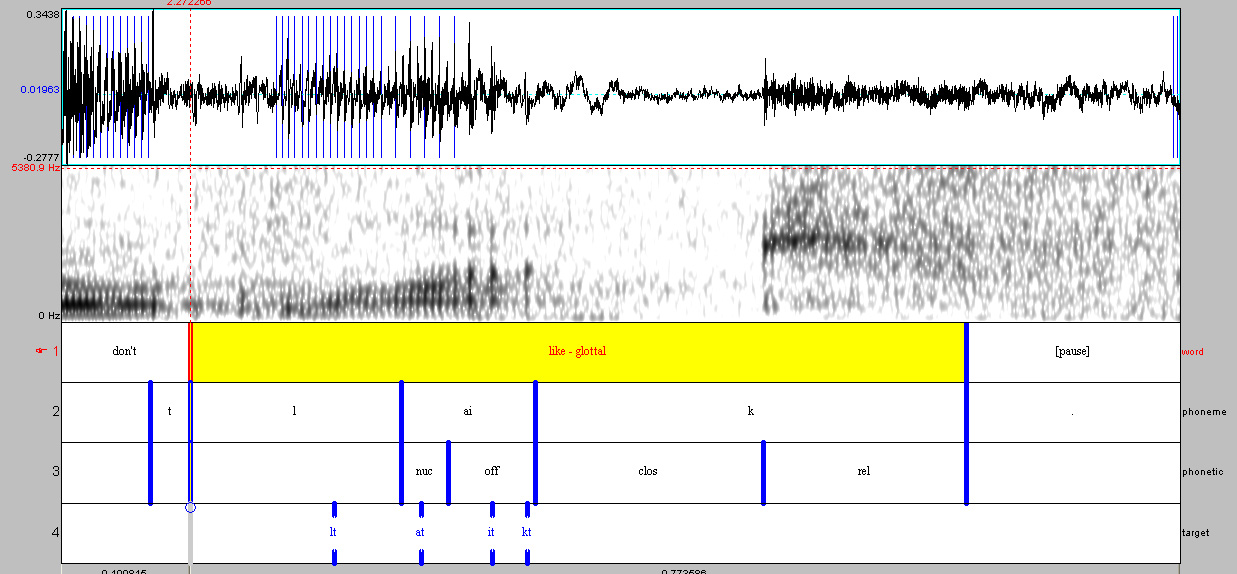
\includegraphics[width=5in]{images/469santra.jpg}
		\caption{Lexical verb \textit{like} from Santra (\isi{The Goths}). \isi{/l/} present, diph\-thongal vowel, glottalised, \isi{/k/} released, preceded by stop, followed by pause} 
	\label{fig:469santra}
\end{figure}

\begin{figure}[p]
	\centering
		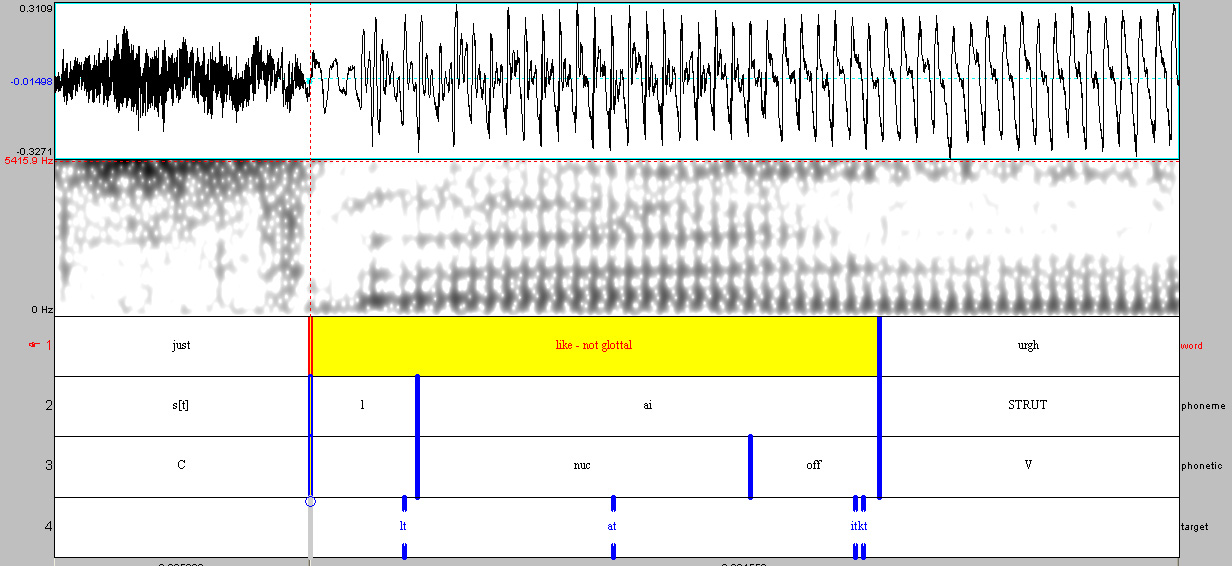
\includegraphics[width=5in]{images/patricia74.jpg}
	\caption{Quotative \textit{like} from Patricia (Sporty Girls). \isi{/l/} present, diph\-thongal vowel, not glottalised, \isi{/k/} absent, preceded by fricative, followed by vowel}
	\label{fig:patricia74}
\end{figure}

\begin{figure}[p]
	\centering
		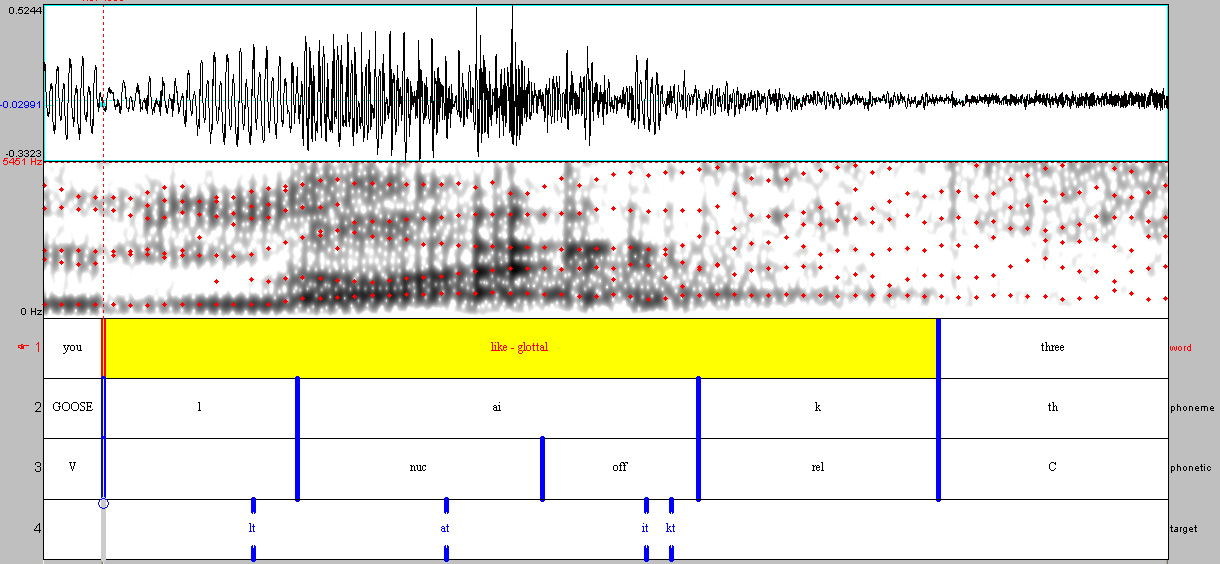
\includegraphics[width=5in]{images/barbara19.jpg}
	\caption{Adverbial \textit{like} from Barbara (\isi{The Relaxed Group}). \isi{/l/} pre\-sent, diph\-thongal vowel, glottalised, fricated \isi{/k/}, preceded by vowel, followed by fricative}
	\label{fig:barbara19}
\end{figure}

\begin{figure}[p]
	\centering
		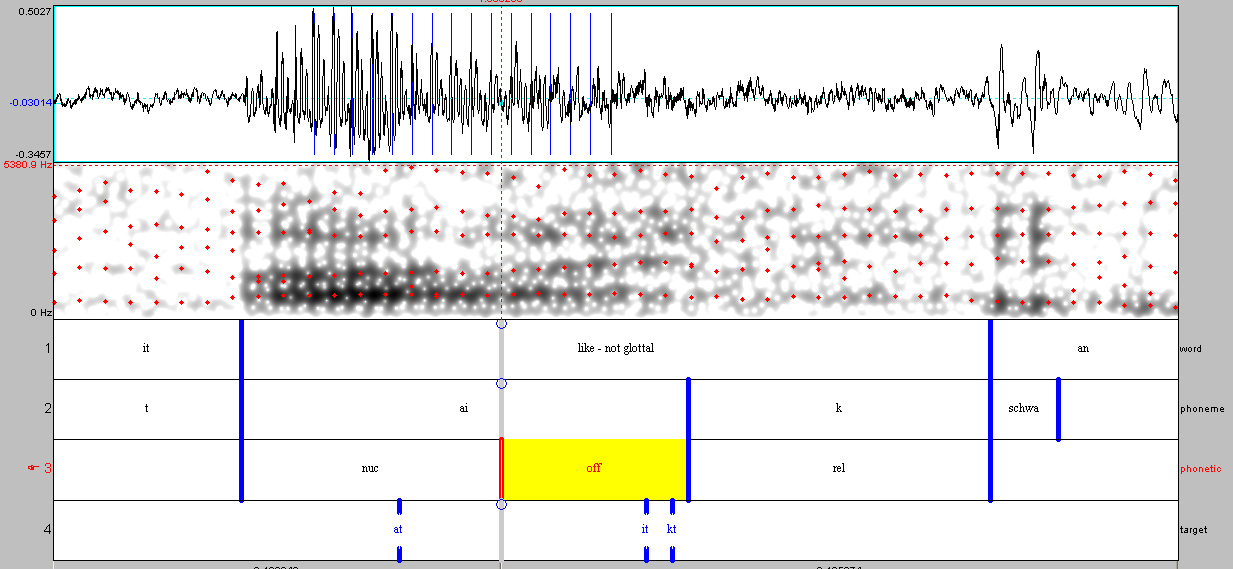
\includegraphics[width=5in]{images/jane37.jpg}
	\caption{Adverbial \textit{like} from Jane (\isi{The BBs}). \isi{/l/} absent, diphthongal vowel, not glottalised, fricated \isi{/k/}, preceded by stop, followed by vowel}
	\label{fig:jane37}
\end{figure}

\begin{figure}[p]
	\centering
		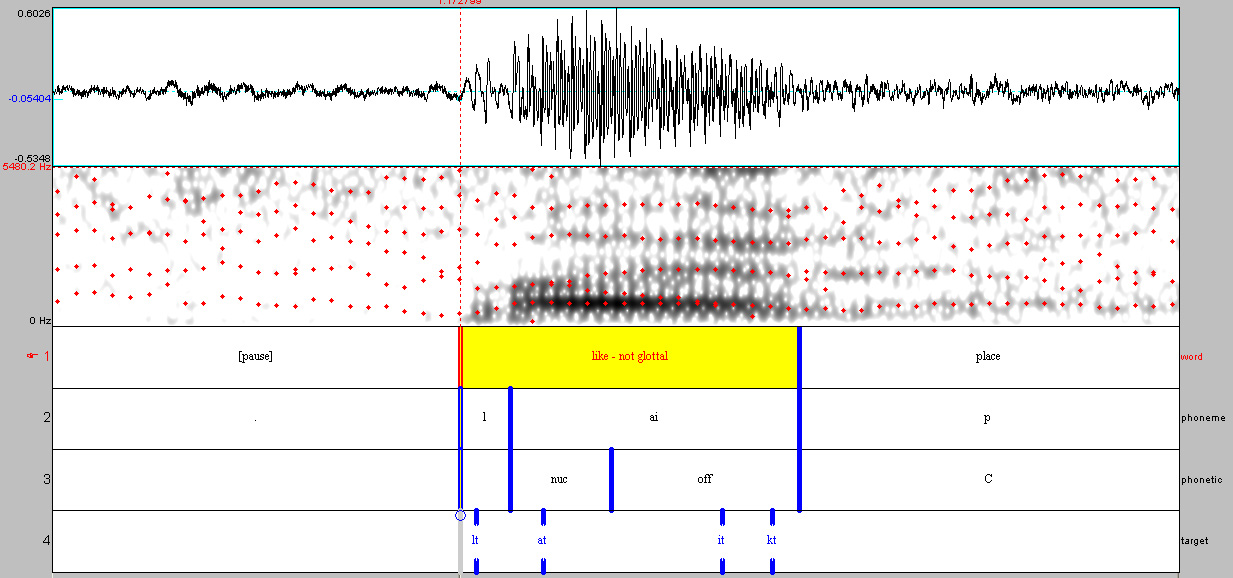
\includegraphics[width=5in]{images/rochelle2.jpg}
	\caption{Discourse particle \textit{like} from Rochelle (Rochelle's Group). \isi{/l/} present, diphthongal vowel, not glottalised, \isi{/k/} absent, preceded by pause, followed by stop}
	\label{fig:rochelle2}
\end{figure}

\begin{figure}[p]
	\centering
		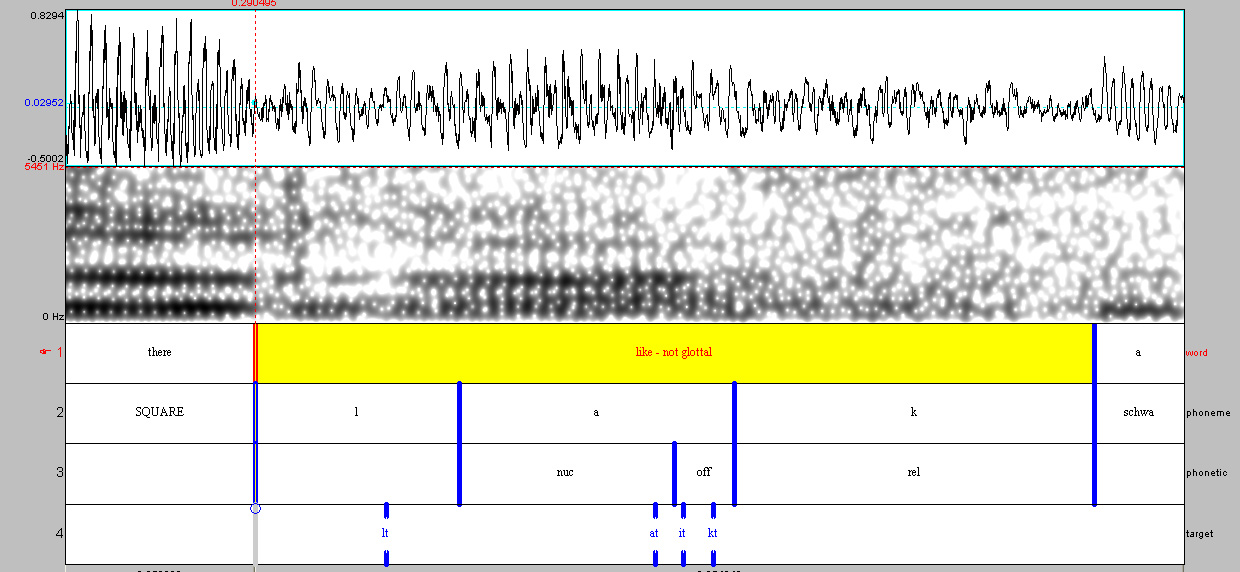
\includegraphics[width=5in]{images/brenda15.jpg}
	\caption{Discourse particle \textit{like} from Marama (\isi{The Pasifika Group}). \isi{/l/} present, monophthongal vowel, not glottalised, fricated \isi{/k/}, preceded by vowel, followed by vowel}
	\label{fig:brenda15}
\end{figure}





Tokens that were followed by a velar consonant were not included in the analysis. The preceding and following pho\-nemes were marked in the text\-grids, with an additional level distinguishing only between vowels, consonants, and pauses. Pauses were labelled as such when a phone did not immediately follow a token of \textit{like}. Voiced continuants, such as \textipa{/l/}, were labelled as consonants. For counts of phonetic features in the raw data, refer to Appendix \ref{appen:proddata}. 


After completion, the textgrids were converted into files that could be read by Emu \citep{emu}. In Emu, \isi{formant traces} were corrected by hand. The formant values were extracted automatically along with other encoded information (e.g., segment duration and whether the token contained a released \isi{/k/}) using a tailor-made library in the statistical software package, R (R Development Core Team 2007). 

Target values of the nucleus and offglide were converted from Hertz to Bark using the equation posited by \citet{traunmuller1990} and the Euclidean di\isi{stance} of a token's vowel was calculated using these \isi{F1} and \isi{F2} values of the nucleus and offglide targets.\footnote{For formant values, the Bark scale was used instead of Hertz because it is a better reflection of how formants at the different frequencies are perceived by human listeners. For example, a shift in \isi{F1} is perceived as greater than a shift in \isi{F2} of the same amount in Hertz.} A completely monophthongal vowel would have a Euclidean di\isi{stance} value of zero, whereas a value of five Bark would be extremely diphthongal. Euclidean di\isi{stance} can therefore be viewed as a gradient measure of how diphthongal a vowel is; the greater the Euclidean di\isi{stance}, the more diphthongal the token. 
\nocite{r}


A token's \isi{pitch} was extracted automatically at 10ms intervals throughout the vowel using the AMDF method in Emu. The mean \isi{pitch} for each token was calculated from the extracted values. Pitch measurements at the nucleus and offglide targets were also extracted and they were used to determine whether a token had a steady or moving \isi{intonation}. Tokens with a transition of 10Hz or more were labelled as `moving'. Due to limits on time, \isi{pitch} contours were not corrected by hand in Emu, so results regarding \isi{pitch} should be viewed with some caution. In order to keep them from biasing results, tokens with a mean \isi{pitch} that was over two standard deviations away from the mean were assigned the \isi{pitch} value at the cutoff point. 



\subsection{Results}\label{sec:prodresults}
%Preliminary analysis revealed that quotative \textit{like} behaved differently from the other functions of \textit{like} with a number of different phonetic variables.  An analysis of these factors will be presented in \sectref{section:quotenonquote}.  Additional differences were found between discourse particle \textit{like} and grammatical functions of \textit{like}.  These differences will be discussed in \sectref{discpgram}. 

The raw data is presented in Appendix \ref{appen:proddata}, with the numbers of different tokens with each phonetic characteristic listed according to whether the speaker was a CR or a NCR girl. Because each of the factors is best understood within the context of all of the other factors, the results are presented in this chapter within the context of statistical models.

In order to test the relationship between the function of \textit{like} and numerous phonetic factors, three mixed effects models were fit to the production data. Like simple linear and logistic regression models, a \isi{mixed effects model} allows for numerous predicting factors to be included in a single model. Significance levels and the degree of each effect are calculated whilst keeping the other factors constant. This effectively takes into consideration the influence of the other variables when investigating a particular factor. For example, assume \isi{/k/} realisation only patterns systematically with following environment (e.g., it is more likely to be realised when followed by a vowel) and following environment predicts the dependent variable being tested. This could lead to \isi{/k/} realisation appearing to be a predicting factor of the dependent variable if following environment is not included in the model. 

Another benefit of using mixed effects models is that in addition to allowing the inclusion of fixed effects, such as phonetic and social factors that can systematically predict the form of the dependent variable, random (non-generalisable) effects can be included \citep[263-326]{baayen2008}.  Random effects can be speaker-specific effects or, in experimental work, stimuli-specific effects. For example, in an analysis of reaction time, some participants may be faster than others. If the researcher wants to examine predicting factors above and beyond this participant-specific effect, they could include the participant as a random effect in the model. Including the speaker as a random effect reduces the risk that a single individual will bias results.\footnote{The random effects included in these models were random intercepts. Random slopes were tested but did not change the reported trends, so the simpler models are included.} 

The first model presented in this chapter compares realisations of quotative \textit{like} to grammatical functions of \textit{like}. The second compares realisations of quotative \textit{like} to discourse particle \textit{like}, and the third compares realisations of the discourse particle to grammatical functions of \textit{like}. A summary of results of all three models can be found at the end of the section in \tabref{tab:sumprodresults}. 

\subsubsection{Model 1: Grammatical and quotative \textit{like}}

Using R, a \isi{mixed effects model} was fit to the data comparing the quotative with grammatical functions of \textit{like}, modeling the likelihood that the token was the quotative. The speaker was included as a random intercept. Before fitting the model, I assumed an alpha level of 0.05 as the threshold for statistical significance. 

A number of factors were tested as potential effects in the model, including vowel duration, preceding and following environment, the different calculations of \isi{pitch} (mean \isi{pitch} and steady versus moving \isi{pitch}), and the \isi{speech rate} (calculated as syllables per second in both the 5 seconds and 20 seconds of speech surrounding a token).\footnote{Only speech that was produced by the same speaker who produced the tokens was used to calculate \isi{speech rate}.} Also tested was whether the speaker was a girl who ate lunch in the CR, whether the \isi{/k/} and \isi{/l/} were realised, the duration of the closure period of the \isi{/k/}, and linear as well as non-linear distributions of the Euclidean di\isi{stance} of a token's vowel. In order to determine whether the probability of a speaker using quotative \textit{like} played a role, tested in the model were interactions between phonetic factors and the two calculations of an individual's use of \textit{like}: the number of tokens of quotative \textit{like} per hundred words produced by that speaker and the percentage of all quotatives produced by an individual that were quotative \textit{like}.\footnote{Both calculations were tested to determine whether they had any power in predicting the relationship between function and phonetic form, both to inform future work in this area and because they have different theoretical implications. The number of tokens of quotative \textit{like} per hundred words failed to reach significance in the model when in place of the second calculation (p$>$0.1).} The number of tokens of the discourse particle observed for each girl per hundred words produced but was not found to reach significance. Factors reaching significance were included as fixed effects in the model, but some factors that approach significance (p$<$0.06) are included in the models in order to account for the variation they appear to be predicting (thereby creating a better fit model). The model's fixed effects and their coefficients for the test variables are shown in \tabref{qgcoeffProd}, and the \isi{control variables} from the model are shown in \tabref{qgcoeffProd-control}.\footnote{The final model was also fit only to data from girls who had ten or more quotatives (see \tabref{tab:percentlike}). All factors reached the same level of significance as in the model reported here. Similarly, the final model was fit first only comparing the quotative with the lexical verb and then comparing it with the adverb. All effects reached significance and were in the same direction as the model presented here with the exception of the value of \isi{F2}, which did not reach significance in either of the models. This provides additional evidence that the lexical verb and the adverb were similar phonetically.} The estimated scale parameter of a model is a measure of how much of the actual variance in the data can be accounted for by the model. Ideally, it is close to 1. The estimated scale parameter for this model is 1.030892, which indicates that it is a good fit.
 

% latex table generated in R 2.6.1 by xtable 1.5-2 package
% Thu Aug 14 10:32:25 2008
\begin{table} [t]
\begin{center}
\begin{tabular}{ld{5}d{2}d{2}d{5}}
  \lsptoprule
 & \multicolumn{1}{r}{Estimate} & \multicolumn{1}{r}{Std. Error} & \multicolumn{1}{r}{z value} & \multicolumn{1}{r}{Pr($>$$|$z$|$)} \\
  \midrule  
  
(Intercept)      &  0.3366 &  0.68  & 0.50 & 0.6198 \\
DIPH             &  -0.4367  & 0.13  & -3.46 & 0.0005 \\
PITCH            &  0.0072 &  0.00  &  3.51 & 0.0005 \\
LV DURATION      &  -2.2391 &  0.59  & -3.81 & 0.0001 \\
   \lspbottomrule
\end{tabular}
\caption{Coefficients of fixed effects for Model 1, comparing the quotative with grammatical functions of \textit{like}}
\label{qgcoeffProd}
\end{center}
\end{table}


\begin{table} 
\begin{center}
\begin{tabular}{ld{5}d{2}d{2}d{5}}
  \lsptoprule
 & \multicolumn{1}{r}{Estimate} & \multicolumn{1}{r}{Std. Error} & \multicolumn{1}{r}{z value} & \multicolumn{1}{r}{Pr($>$$|$z$|$)} \\
  \midrule  
preceded by pause        &  -0.8199  & 0.87 & -0.94 & 0.3482 \\ 
preceded by fricative  		& 1.7364 &  0.28  & 6.21 & <0.0001 \\
followed by pause         &  0.8526 &  0.52  & 1.64 & 0.1015 \\
followed by V             &  -0.1981 &  0.42 & -0.47 & 0.6379 \\
followed by sibilant        & -1.8554  & 0.65  & -2.87 & 0.0041 \\
followed by nasal           & -1.0028  & 0.55  & -1.81 & 0.0697 \\
followed by other voiceless  & -1.8175 &  0.51 & -3.53 & 0.0004 \\
followed by other voiced     & -3.1986 &  0.57 & -5.65 & <0.0001 \\
   \lspbottomrule
\end{tabular}
\caption{Coefficients of \isi{control variables} for Model 1, comparing the quotative with grammatical functions of \textit{like}}
\label{qgcoeffProd-control}
\end{center}
\end{table}



Fixed effects in the model include the preceding and following environment, the Euclidean di\isi{stance} between \isi{F1} and \isi{F2} of the nucleus and offglide as a measure of how diphthongal the token's vowel was (DIPH), the mean \isi{pitch} (PITCH), and the ratio of \isi{/l/} to vowel duration (LV DURATION). 
 
The defaults of the model are that the token was preceded by something other than a fricative or a pause and was followed by a consonant (followed by C). For continuous factors, the model assumes a value of zero, even when this value is not present in the data. Therefore, the model assumes as a default that the vowel was completely monophthongal (DIPH = 0) and that the \isi{/l/} to vowel duration ratio was zero (LV DURATION = 0), both of which are values that were observed in the data. Tokens with an \isi{/l/} to vowel duration ratio of zero were tokens where there was no acoustic evidence of an \isi{/l/}; the \isi{/l/} was dropped. The intercept's estimate given in \tabref{qgcoeffProd} is the likelihood in log odds that a token with the default characteristics was quotative \textit{like}. To determine the log odds for tokens that do not match the default criteria, the estimate for binary factors must be added to the default intercept of the model. For example, to determine the likelihood that a token was quotative \textit{like} if it had the default characteristics except that it was followed by a pause, the estimate for tokens followed by pauses (-0.8199) would be added to the estimated intercept (0.3366). For continuous factors, such as Euclidean di\isi{stance}, the product of the factor's coefficient and the token's Euclidean di\isi{stance} is added to the estimated coefficient of the intercept. In calculating log odds of factors for the graphs presented in this chapter, the mean values of continuous factors were used as defaults.

Prior to running the final model, the different preceding environments were run as separate factors in the factor group for the preceding environment.\footnote{First, the different phonemes which preceded each token were treated as factors. They were then divided depending on voicing and on whether they were continuous. Whether a token was continuous did not significantly predict the function of \textit{like}. Voiceless tokens were less likely to precede the quotative than the grammatical function (p$<$0.05), but there is no interaction between voicing and whether the preceding environment was a fricative. This makes it unlikely that the shorter \isi{/l/} to vowel duration ratio associated with the quotative was due to identifying portions of the \isi{/l/} that were voiceless (as a result of coarticulation) as the preceding segment.} They appeared to clump according to whether they were a fricative, a pause, or something else. Therefore, the factor group for the preceding environment that was included in the final model had this three-way distinction. As indicated by the positive coefficient in \tabref{qgcoeffProd}, tokens that were preceded by a fricative were significantly more likely to be the quotative than a grammatical function when compared to tokens that were preceded by a segment that was non-fricated (p$<$0.0001). Although there was not a significant difference between tokens that were preceded by a pause and by a non-fricated segment, these factors were not collapsed into a single factor in order to maintain consistency across the different production models.

For the factor group of following environment, the model was first tested with each phoneme listed as a separate factor (e.g., /f/, /b/, pause). The following environment was divided into seven discrete factors: followed by an approximant, followed by a pause, a vowel, a sibilant, a nasal, by some other segment that was voiceless, and by some other segment that was voiced. The preceding environment was divided into three discrete factors: preceded by a pause, preceded by a fricative, and preceded by anything else. The model held the fixed effect of following environment constant when testing the other factors, so the predicted effect of other factors was independent from following environment. 

A token was significantly less likely to be quotative \textit{like} if it was more diphthongal (p$<$0.001). The higher the Euclidean di\isi{stance} of a vowel, the less likely it was to be the quotative. This was a continuous factor and its relationship with the function of \textit{like} was also continuous; tokens with vowels that were more diphthongal were more likely to be a grammatical function of \textit{like}.  

\largerpage
A vowel's mean \isi{pitch} also significantly predicted whether or not a token was the quotative. The higher the mean \isi{pitch}, the more likely it was that the token was quotative \textit{like} as opposed to a traditionally grammatical function of \textit{like} (p$<$0.001). This is likely related to the prosodic position in a sentence of the different types of \textit{like}. Though both lexical verb \textit{like} and quotative \textit{like} function as verbs, their syntactic properties differ, affecting their position in a sentence. Impressionistically, lexical verb \textit{like} seemed to be produced in conjunction with a dip in the \isi{intonation} contour, whereas quotative \textit{like} rarely was and was sometimes part of a rising contour that raised more steeply after the verb. 

Tokens with a larger \isi{/l/} to vowel ratio have a longer \isi{/l/} duration relative to the duration of the vowel. These tokens with a relatively long \isi{/l/} were significantly less likely to be quotative \textit{like} than a grammatical function of \textit{like} (p$=$0.0001). Though measures of \isi{speech rate} failed to reach significance in differentiating between the functions of \textit{like}, using the ratio of \isi{/l/} to vowel duration helped to normalise the duration of \isi{/l/} across different rates of speech. That the ratio reached significance in the model suggests that the relationship between \isi{/l/} duration and function of \textit{like} was not an artefact of different speech rates across the different functions.  



\subsubsection{Model 2: Quotative and discourse particle \textit{like}}

A \isi{mixed effects model} comparing tokens of the quotative with tokens of the discourse particle was fit to the data, modeling the likelihood that a particular token of \textit{like} was the quotative. As with the first model, speaker was included as a random effect. The same factors as tested in model 1 were tested in model 2. Only those reaching significance were included in the model. These included how diphthongal the token was, the ratio of \isi{/l/} to vowel duration, the mean \isi{pitch} of the token, and the preceding and following environment as described for the previous model. Also reaching significance in the model was an interaction between whether or not the \isi{/k/} was dropped and whether the girl was in a group who ate lunch in the CR. Speech rate, frequency of use of quotative and discourse particle \textit{like}, and whether the token had a steady \isi{intonation} contour failed to reach significance and were not included in the model. The coefficient table for the production model is shown in \tabref{qdpcoeffProd}. 
 
 

% latex table generated in R 2.6.1 by xtable 1.5-2 package
% Thu Aug 14 09:54:29 2008
\begin{table}[p]
\begin{center}
\begin{tabular}{ld{5}d{2}d{2}d{5}}
  \lsptoprule
 & \multicolumn{1}{r}{Estimate} & \multicolumn{1}{r}{Std. Error} & \multicolumn{1}{r}{z value} & \multicolumn{1}{r}{Pr($>$$|$z$|$)} \\
  \midrule

(Intercept)   &  -0.4093 &  0.56  & -0.735 & 0.4626 \\
  DIPH        &  -0.4671 &  0.11  & -4.212 &  <0.0001 \\
  PITCH       &  0.0079  & 0.00   & 4.501  & <0.0001 \\
  LV DURATION &  -1.4819 &  0.49  & -3.024 & 0.0025 \\
  K-CLOS=N    &  -0.9035 &  0.30 & -2.987 & 0.0028 \\
  GROUP=NCR   &  -0.5364 &  0.34  & -1.560 & 0.1187 \\
  K-CLOS=N:GROUP=NCR  &  1.3050  & 0.44  & 2.97 & 0.0029 \\

   \lspbottomrule
\end{tabular}
\caption{Coefficients of fixed effects for Model 2, comparing the quotative with the discourse particle}
\label{qdpcoeffProd}
\end{center}
\end{table}
  


 
% latex table generated in R 2.6.1 by xtable 1.5-2 package
% Thu Aug 14 09:54:29 2008
\begin{table}[p]
\begin{center}
\begin{tabular}{ld{5}d{2}d{2}d{5}}
  \lsptoprule
 & \multicolumn{1}{r}{Estimate} & \multicolumn{1}{r}{Std. Error} & \multicolumn{1}{r}{z value} & \multicolumn{1}{r}{Pr($>$$|$z$|$)} \\
  \midrule
  preceded by pause     &  -2.8558 &  0.76 & -3.78 & 0.0002 \\
  preceded by fricative  &  0.8261  & 0.22 &   3.78 & 0.0002 \\
  followed by pause     &  0.0618  & 0.33  & 0.19 & 0.8516 \\
  followed by V         &  0.4689  & 0.32  & 1.45 &  0.1470  \\
  followed by sibilant  & -0.4713 & 0.59  & -0.80 &  0.4253 \\
	followed by nasal   & 0.3668   & 0.48  & 0.76 &  0.4475 \\
	followed by other voiceless  & -0.6591 &  0.42 & -1.56 & 0.1179 \\
	followed by other voiced   & -1.7862  & 0.51 & -3.50 & 0.0005 \\   
	
	\lspbottomrule
\end{tabular}
\caption{Coefficients of \isi{control variables} for Model 2, comparing the quotative with the discourse particle}
\label{qdpcoeffProd-control}
\end{center}
\end{table}


 
A token was less likely to be a quotative if preceded by a pause than if preceded by a fricative (p$<$0.0001) or any other segment (p$<$0.001). A token was more likely to be a quotative if preceded by a fricative than if preceded by any other segment (p$<$0.001).

 
A token's Euclidean di\isi{stance} also predicts the function of a token. A token was significantly more likely to be quotative \textit{like} if it was more monophthongal (p$<$0.0001), as indicated by the negative coefficient value. This is also similar to results from model 1. 

As with the first model, a token with a higher mean \isi{pitch} was more likely to be quotative \textit{like} (p$<$0.0001). Again, this is likely related to the words' prosodic position in a sentence. Tokens of quotative \textit{like} were often followed by reported speech in a very high \isi{pitch}, and the token of quotative \textit{like} itself rarely had the lowest \isi{pitch} in the phrase. Discourse particle \textit{like}, on the other hand, was produced in conjunction with a dip in the \isi{intonation} contour. It could have a very low \isi{pitch} and was often produced with a creaky quality.

\largerpage
As in model 1, a token with a long \isi{/l/} duration relative to its vowel duration was less likely to be quotative \textit{like} than to be discourse particle \textit{like} (p$<$0.01). This provides evidence that quotative \textit{like} had a shorter \isi{/l/} duration, regardless of \isi{speech rate}. Similar results were found in model 1, suggesting that quotative \textit{like} was most likely to have a shorter duration ratio, regardless of the non-quotative function with which it was paired.


The model includes a significant interaction between whether the \isi{/k/} in a token was realised or not and whether the girl who produced the token was a CR girl or not (p$<$0.01).\footnote{The interaction remains significant if the duration of the \isi{/k/ closure} is included in the model in place of the discrete measure of whether or not the \isi{/k/} was realised. Because the effect appeared to be carried entirely by the tokens where the closure duration was equal to zero as opposed to all other closure durations, the discrete measure was used in the model.} A token where the \isi{/k/} was dropped was more likely to be quotative \textit{like} if produced by a CR girl, but less likely to be quotative \textit{like} if produced by a NCR girl.\footnote{The significance level presented here is for the interaction between CR and \isi{/k/} realisation. Separate models fit first to the CR girls' data and then to the \isi{NCR girls}' data, reveal that while the trend with \isi{/k/} realisation is significant for the CR girls (p$<$0.05), it is not significant for the \isi{NCR girls} (p$>$0.7). The arguments presented in this chapter are based on the opposite trends found for the two groups, which is why the interaction's significance level and coefficient are the focus of this discussion.} This interaction, shown in \figref{fig:kCR-qdp}, was independent of following environment, as following environment was included as a fixed effect in the model. It seems there were not only differences in pronunciation between the different types of \textit{like} but that different \isi{social groups} had different realisations for the different functions of \textit{like}. 
\begin{figure}[t]
	\centering
		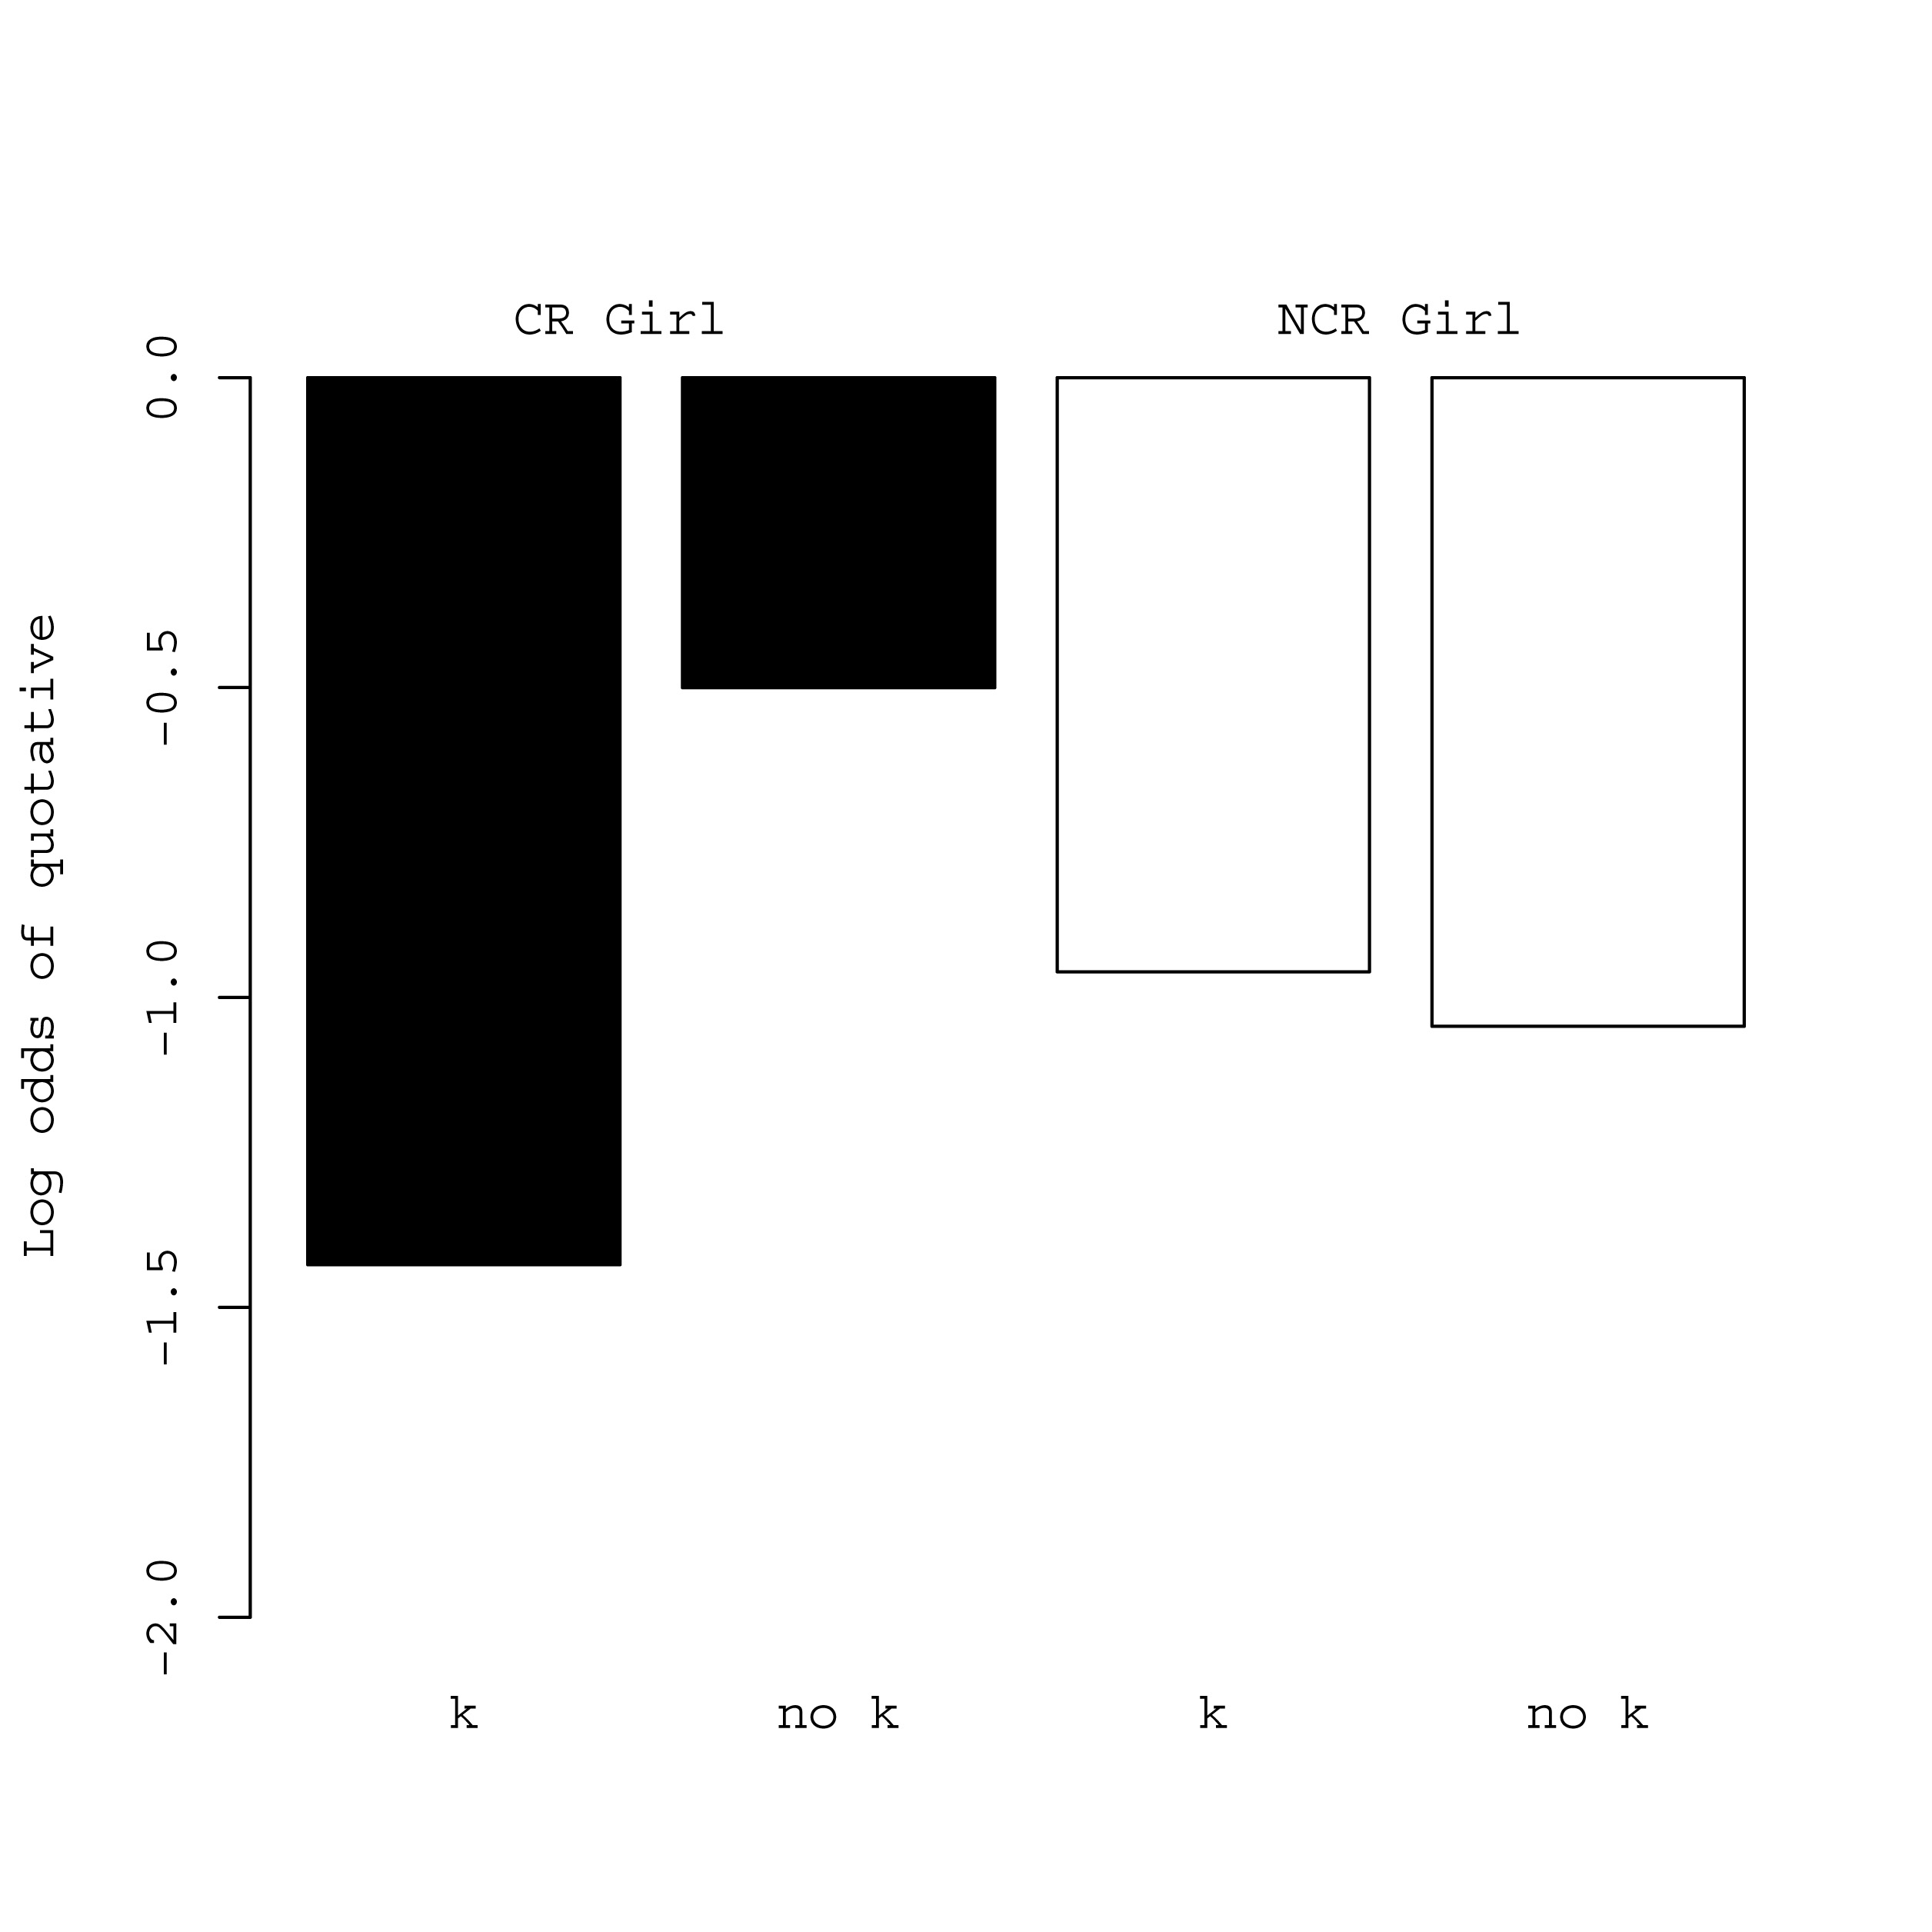
\includegraphics[height=.4\textheight]{images/kCR.jpg}
	\caption{Graph of the interaction between whether the \isi{/k/} was realised and whether the speaker was in a group who ate lunch in the CR (black) or not (white). The graph is based on the model's predictions. A higher value (i.e. closer to zero) on the y-axis indicates a greater likelihood that the token was quotative \textit{like}.}
	\label{fig:kCR-qdp}
\end{figure}





%no luck with eps, why???
%\begin{figure}
%\epsfxsize0.9\textwidth
%\epsffile{images/kCR.ps}
%\caption{Graph of interaction based on model's predictions of likelihood of quotative \textit{like} depending on whether the \isi{/k/} is realised and whether the speaker is in a group who eats lunch in the Common Room (CR, blue) or not (NCR, red)}. \label{prodinteract}
%\end{figure} 
%\epsfbox{kCR.eps}  this doesn't work either...


This interaction was not carried exclusively by quotative \textit{like}; the opposite trend of \isi{/k/} realisation was found for the discourse particle. While CR girls were more likely to produce the \isi{/k/} in discourse particle \textit{like}, \isi{NCR girls} were more likely to drop the \isi{/k/}.

This interaction is not an artefact of the frequency of use of either the quotative or the discourse particle. Though they do not reach significance in the model, if frequency measures are included, the interaction between \isi{/k/} realisation and a girl's eating place is still significant. This provides statistical evidence that the interaction is independent of the speaker-specific probability of producing quotative \textit{like}. Interestingly, CR girls were significantly more likely to use the discourse particle than \isi{NCR girls} (Wilcoxon, p$=$0.01).\footnote{This is based on the calculation presented in \sectref{section:dplike}.} But there is no interaction between the frequency of use of the discourse particle and whether the \isi{/k/} is realised.\footnote{This was tested with the percentage of all words that were the discourse particle, the percentage of all tokens of \textit{like} that were the discourse particle, and the ratio of quotative to discourse particle tokens produced by a speaker.} Irrespective of how often a girl used quotative and discourse particle \textit{like}, she was more likely to realise the \isi{/k/} in quotative \textit{like} than in discourse particle \textit{like} if she was a NCR girl and more likely to drop the \isi{/k/} in the quotative than in the discourse particle if she was a CR girl. For example, Juliet (PCs), Barbara (Relaxed Group), and Clementine (Trendy Alternatives) were all CR girls who were not particularly frequent users of quotative \textit{like} and they produced the \isi{/k/} more frequently in quotative \textit{like} than did some of their friends who used quotative \textit{like} more often. However, these girls were more likely to produce the \isi{/k/} in the discourse particle than in the quotative, thereby patterning more similarly to their CR friends than with \isi{NCR girls} who were also infrequent users of quotative \textit{like}. 



%I first observed this trend in the speech of Onya, who is a central member of the most rebellious group, \isi{The Real Teenagers}. In order to find out whether other \isi{NCR girls} also followed this trend, Onya's speech was not included in the model.

%\subsection{Quality of \textipa{/ai/}}


In regard to monophthongisation, mean \isi{pitch}, \isi{/l/} to vowel duration ratio, and following environment, both discourse particle \textit{like} and grammatical functions of \textit{like} behaved similarly when compared to quotative \textit{like}. However, they involved different interactions: one with \isi{/k/} realisation and the speaker-specific probability of a token, and the other with \isi{/k/} realisation and the social grouping of the speaker. Whereas the realisation of \isi{/k/} was linked to frequency of use for quotative \textit{like}, it did not appear to be linked to frequency of use for the discourse particle. Phonetic differences between grammatical functions of \textit{like} and the discourse particle will be presented in the following section.

%The realisation of \isi{/k/} in quotative \textit{like} may be linked both to cognitive processes due to frequency effects and the manipulation of phonetic variables for the construction of \isi{identity}. However, socially-conditioned variation seems to be the only effect for \isi{/k/} realisation in the discourse particle.




\subsubsection{Model 3: Grammatical and discourse particle \textit{like}}


A \isi{mixed effects model} was fit to the data comparing the discourse particle with grammatical functions of \textit{like}, modelling whether a token was one of the traditionally grammatical functions. Speaker was included as a random effect. Coefficients of the model's fixed effects are shown in \tabref{dpgramcoeff} and the model's \isi{control variables} are shown in \tabref{dpgramcoeff-control}. 


% latex table generated in R 2.6.1 by xtable 1.5-2 package
% Mon Aug 11 13:13:39 2008
\begin{table}[b]
\begin{center}
\begin{tabular}{ld{5}d{5}d{2}d{5}}
  \lsptoprule
 & \multicolumn{1}{r}{Estimate} & \multicolumn{1}{r}{Std. Error} & \multicolumn{1}{r}{z value} & \multicolumn{1}{r}{Pr($>$$|$z$|$)} \\
  \midrule
(Intercept)    &  4.8433  &  1.8126 &  2.67&  0.0075\\ 
NUC \isi{F2}       &  -0.4876 &  0.1546 & -3.15& 0.0016 \\ 
LV DURATION       &  -0.2231 &  0.6144 & -0.36& 0.7165 \\
GROUP=NCR                 &-0.4758   &  0.4666 & -1.02& 0.3079 \\ 
LV DURATION:GROUP=NCR     &  1.7159  &  0.8670 &  1.98& 0.0478 \\  
   \lspbottomrule
\end{tabular}
\caption{Coefficients of fixed effects for Model 3, comparing the discourse particle with grammatical functions of \textit{like}}
\label{dpgramcoeff}
\end{center}
\end{table}

% latex table generated in R 2.6.1 by xtable 1.5-2 package
% Mon Aug 11 13:13:39 2008
\begin{table}[b]
\begin{center}
\begin{tabular}{ld{5}d{5}d{2}d{5}}
  \lsptoprule
 & \multicolumn{1}{r}{Estimate} & \multicolumn{1}{r}{Std. Error} & \multicolumn{1}{r}{z value} & \multicolumn{1}{r}{Pr($>$$|$z$|$)} \\
  \midrule

preceded by pause  & -1.7516  & 0.3915 & -4.475 & <0.0001 \\
preceded by fricative 	& -0.9553   &  0.2503 & -3.82 & 0.0001 \\
followed by pause     &  -0.8570   &  0.4843  & -1.77 & 0.0768 \\
followed by V    &  0.7412 &    0.3799 &  1.95 & 0.0510 \\
followed by sibilant   & 1.4890  &   0.5040   & 2.95   & 0.0031 \\
followed by nasal    & 1.2666  &   0.5062   & 2.50 & 0.0123 \\
followed by other voiceless & 0.8749   &  0.4058 &  2.16 & 0.0311 \\
followed by other voiced  & 1.3631     & 0.3854   & 3.54 & 0.0004 \\  

   \lspbottomrule
\end{tabular}
\caption{Coefficients of \isi{control variables} for Model 3, comparing the discourse particle with grammatical functions of \textit{like}}
\label{dpgramcoeff-control}
\end{center}
\end{table}


\noindent The preceding and following environment and the \isi{F2} value of a token's nucleus target significantly predicted whether a token was a grammatical function. A token that was preceded by a pause or a fricative was less likely to be a grammatical function of \textit{like} than the discourse particle when compared with a token preceded by some other segment (p$<$0.0001). The difference between tokens preceded by a pause as opposed to a fricative was approaching significance (p$=$0.06), with tokens preceded by a fricative being more likely to be a grammatical function. 

Tokens that were followed by an approximant were significantly less likely to be a grammatical function of \textit{like} than tokens that were followed by a sibilant (p$<$0.001), a nasal (p$<$0.05), a voiceless consonant of a different manner of articulation (p$<$0.05), and a voiced consonant of a different manner of articulation (p$<$0.001). 

Tokens with a higher \isi{F2} at the target of the nucleus (i.e. tokens with a nucleus that was less back) were less likely to be a grammatical function of \textit{like} (p$<$0.01). This suggests that grammatical functions of \textit{like} were more likely to be produced with a backer \isi{diphthong} nucleus than the discourse particle. Between the two discursive functions, there was no significant difference in \isi{F2}.

Also reaching significance in the model is an interaction between the \isi{/l/} to vowel duration ratio and whether or not the speaker ate lunch in the Common Room (p$<$0.05); tokens with a long \isi{/l/} relative to the vowel were more likely to be the discourse particle if produced by a common room girl and were more likely to be one of the grammatical functions if produced by a non-common room girl. Together with the interaction from model 2, the results suggest that a word's phonetic realisation can depend on a combination of the word's grammatical function and the social characteristics of the speaker who produced it.

%  In \isi{NZE}, the PRICE \isi{diphthong} is un with a backer nucleus are considered more innovative  \citep{onzebook}.  This provides evidence that grammatical \textit{like} was more likely to be produced with a more innovative realisation than the discourse particle.  

A summary of results from all three models is presented in \tabref{tab:sumprodresults}.

  
\begin{table}
\begin{center}
\begin{tabular}{lr}
  \lsptoprule
 type & summary of traits \\
 \midrule
 
 grammatical & low \isi{pitch}   \\
             & more diphthongal \\
             & long \isi{/l/} to vowel duration ratio \\
             & shorter \isi{/l/} to vowel duration ratio for CR girls \\
             
             \midrule
 quotative   & high \isi{pitch} \\
             & less diphthongal \\
             & short \isi{/l/} to vowel duration ratio \\
             & more \isi{/k/} reduction for CR girls than \isi{NCR girls} \\
             \midrule
             
 discourse particle & low \isi{pitch} \\
        		 & large \isi{F2} value but still diphthongal \\
             & long \isi{/l/} to vowel duration ratio \\
             & shorter \isi{/l/} to vowel duration ratio for \isi{NCR girls} \\
             & more \isi{/k/} reduction for \isi{NCR girls} than CR girls \\
  \lspbottomrule

\end{tabular}
\caption{Summary of results from the first three statistical models}
\label{tab:sumprodresults}
\end{center}
\end{table}


\section{Discussion}\label{sec:proddisc}

The results provide evidence that different functions of \textit{like} have different realisations.\footnote{It is possible that some of the variation observed between functions is due to effects of \isi{prosody} and other phonetic cues not investigated here. This is discussed briefly in \sectref{sec:prosody}.} The ultimate realisation depends on a combination of a token's grammatical function and the social grouping of the girl who produced it. That the girls' realisations of \textit{like} were systematically different depending on the function of a token suggests that these items are stored in the mind in a way that maintains the distinction. This is discussed in Chapter \ref{ch:disc} where I also describe implications of results from the \isi{perception} experiments presented in Chapter \ref{ch:perc}. The current section discusses how the results add to previous work on sound change, the discursive status of certain lexical items, and the link between phonetic reduction and a token's probability given the context. 
% 


\subsection{Frequency effects}
\largerpage[-1]
Previous studies provide evidence that token frequencies correlate with at least some phonetic variables. The majority of previous studies have focused on vowel duration \citep{bybee2001,jurafskyetal2002,gahl-thyme}, but vowel quality and monophthongisation have also been shown to correlate with frequency measures \citep{munson2007,oprah1999}. In these studies, monophthongisation, shorter vowel durations, and a more compact vowel space are associated with tokens that have a higher frequency. In the SGH data, the different measures of relative frequency of use described in \sectref{section:uselike} did not interact with monophthongisation, vowel duration, or the \isi{/l/}-vowel duration ratio. Given the amount of previous work that has found a relationship between \isi{token frequency} and duration, it is surprising that no such effects were observed here. This may be a result of using measurements that reflect the speaker-specific probability of producing a token in a given context (e.g., when speaking, or when producing a quotative) as opposed to an overall approximation of \isi{token frequency}. Alternatively, it may be related to the fact that, across all speakers, all of the analysed functions of \textit{like} would be classified as highly frequent in previous studies. For example, \citet{bybee2002} treats words that are observed in corpus data equal to or more than 35 times per million words as high-frequency; all of the analysed functions of \textit{like} were more frequent than this for all speakers in the SGH data. 

In the model comparing the quotative with the grammatical functions, there is an interaction between \isi{/k/} realisation and the percentage of all quotatives that were quotative \textit{like}. This interaction suggests that the speaker-specific probability of an item in a given context is linked to phonetic reduction in that item. To demonstrate that this effect is independent of the effect of a girl's status as a CR girl or a NCR girl, I have fit a fourth \isi{mixed effects model} with speaker as a random effect, modeling \isi{/k/} realisation and only including tokens of quotative \textit{like}. The model's output is shown for the test items in \tabref{model4coeff} and for the \isi{control variables} in \tabref{model4coeff-control}.

   \begin{table}[t]
\begin{center}
\begin{tabular}{ld{6}d{6}d{3}d{7}}
  \lsptoprule
 & \multicolumn{1}{r}{Estimate} & \multicolumn{1}{r}{Std. Error} & \multicolumn{1}{r}{z value} & \multicolumn{1}{r}{Pr($>$$|$z$|$)}  \\
  \midrule
  
(Intercept)    &  -8.58498  &  3.75172  & -2.288  & 0.02212 \\
DIPH           &  0.92959  &  0.21775  & 4.269 & <0.0001 \\  
LV DURATION &  2.26894  &  0.84877  & 2.673  & 0.00751 \\
NUC \isi{F2}   & 0.77772   & 0.28334  &  2.745 & 0.00605 \\
GROUP=NCR           &  1.47449  &  0.51989  & 2.836 & 0.00457  \\
PROB QUOTE          &  -0.04481  &  0.02160 & -2.075  & 0.03801  \\

   \lspbottomrule
\end{tabular}
\caption{Coefficients of fixed effects for Model 4, modeling \isi{/k/} reduction for tokens of quotative \textit{like}}
\label{model4coeff}
\end{center}
\end{table}

   
         


\begin{table}[t]
\begin{center}
\begin{tabular}{ld{5}d{3}d{3}d{5}}
  \lsptoprule
 & \multicolumn{1}{r}{Estimate} & \multicolumn{1}{r}{Std. Error} & \multicolumn{1}{r}{z value} & \multicolumn{1}{r}{Pr($>$$|$z$|$)}  \\
  \midrule
preceded by pause    &  -2.7829 &   1.78  & -1.57  & 0.1174 \\
preceded by fricative 	& 0.1268  &  0.38 &  0.34 & 0.7360 \\
followed by pause  &  1.1055  &  0.56  & 1.96 & 0.0495 \\
followed by V   &   1.1439 &   0.54 &  2.12 & 0.0341 \\
followed by sibilant & 2.2012  &  1.07 &  2.07 & 0.0389 \\
followed by nasal &  1.1754  &  0.74  & 1.59 & 0.1112 \\
followed by other voiceless & 0.4163 &   0.83 &  0.50 & 0.6156 \\
followed by other voiced  &  17.3702 & 989.60 &  0.02 & 0.9860 \\ 
   \lspbottomrule
\end{tabular}
\caption{Coefficients of \isi{control variables} for Model 4, modeling \isi{/k/} reduction for tokens of quotative \textit{like}}
\label{model4coeff-control}
\end{center}
\end{table}
 
\largerpage[-1]
The model shows that there is a significant relationship between \isi{/k/} realisation and a token's Euclidean di\isi{stance} (p$<$0.0001) and \isi{/k/} realisation and the \isi{/l/} to vowel duration ratio of a token (p$<$0.05). More diphthongal tokens and tokens with a longer \isi{/l/} relative to the vowel were more likely to have the \isi{/k/} present. This is not surprising if monophthongisation, \isi{/l/} duration reduction, and \isi{/k/} dropping are all reductive processes. Tokens that have the \isi{/k/} realised were also more likely to have a higher \isi{F2} at the nucleus target (p$<$0.01).

The key finding in this mo\-del was that for quotative \textit{like} both the spea\-ker's social grouping and how often she used quotative \textit{like} were linked to \isi{/k/} realisation. \isi{NCR girls} were more likely to realise the \isi{/k/} than CR girls (p$<$0.05) and the more a girl used quotative \textit{like}, the less likely she was to realise the \isi{/k/} in it (p$<$0.05). Both social and frequency effects played a role in predicting whether the \isi{/k/} was realised.\footnote{Models fit only to the grammatical tokens and to the discourse particle tokens revealed that the social grouping and \isi{speaker-specific frequency} did not play a significant role in whether or not the \isi{/k/} was realised (p$>$0.1 for the effects in both models).}

%, whereas in model 2, speaker frequencies of quotative and discourse particle \textit{like} do not appear to play a role in predicting \isi{/k/} realisation. The interaction between social group and \isi{/k/} realisation is not an artefact of frequency.  Though there are more documented tokens of the discourse particle in the speech of CR girls than \isi{NCR girls}, frequency of the discourse particle does not reach significance when tested in an interaction in the model. Additionally, given the previous work on reductive processes and frequency of use, we might expect that the CR girls would be less likely to realise the \isi{/k/} in discourse particle \textit{like} than the \isi{NCR girls} because, as disccused in \sectref{tab:diffquotes}, they appear to use the discourse particle more often.  But, if anything, the opposite was observed.  

%Using a larger corpus to test the influence of speaker-specific \isi{token frequency} on sound change and phonetic variation is an interesting avenue for future research. 


Previous work has observed a relationship between the phonetic realisation of a word and its predictability based on contextual information \citep{jurafskyetal2002}: words that are more predictable given the preceding context undergo more reductive processes. These findings help to interpret the results regarding the relationship between \isi{/k/}-dropping and the percentage of a speaker's quotatives that were quotative \textit{like}. If the contextual information indicates that a speaker is likely to produce a quotative, the probability of that quotative being \textit{like} (as opposed to some other quotative) is speaker-dependent. Thus, for speakers who have a high percentage of quotatives that are \textit{like}, \textit{like} is more predictable in its local context; for these speakers, \isi{/k/} is more likely to be dropped. Conversely, for speakers who have a lower percentage of quotatives that are \textit{like}, \textit{like} is less predictable in its local context and the \isi{/k/} is less likely to be dropped.

This supports previous findings that words that are more predictable given the preceding context undergo more reduction. Further, it indicates that predictability needs to be considered at the level of the individual speaker; not all words are equally predictable in all contexts for all speakers.

%If phonetic reduction is more likely to be observed when a word is more likely to occur in a given context, the same cognitive mechanisms would predict that phonetic reduction in an item is more likely to occur if, in a particular context, the likelihood of a speaker producing that item is high. If the contextual information indicates that a speaker is likely to produce a quotative, the probability of producing \textit{like} is speaker-dependent.  The results indicate that when this speaker-specific probability is high, \isi{/k/} is more likely to be dropped.  This provides evidence that, in addition to contextual predictability affecting phonetic realisations, the probability of a particular speaker producing a word in a context also affects phonetic realisations.

\largerpage
It is possible that phonetic patterns that derive from speaker-specific, context-dependent probabilities could be exploited as a stylistic resource. Such re-ap\-pro\-pri\-a\-tion of phonetic variables could have led to the differences in \isi{/k/} realisation observed between CR and \isi{NCR girls}. Stylistic resources are constantly recombined in a process of \isi{bricolage} \citep{hebdige1984,eckert2008}. While work such as that by \citet{milroymilroy1978} has focused on a community or social group's adoption of (and reassignment of meaning to) variables used by another group, it is also possible that phonetic variability originally driven by speaker-specific probabilities could be manipulated for stylistic means. Due to the multidimensional nature of the stylistic components, the model presented in Chapter \ref{ch:disc} predicts that socially-conditioned phonetic variability could arise from probabilistic distributions of the variables based on non-social factors.




%This would be consistent with the predictions of an \isi{exemplar model}, which will be discussed in Chapter \ref{ch:disc}.  

%Another interpretation is that \isi{/k/} dropping is linked to \isi{identity} construction; girls who choose to use quotatives other than quotative \textit{like} may also choose to realise the \isi{/k/} in quotative \textit{like} when they produce it in order to diverge from the more frequently used pronunciation.  This would be consistent with results from Model 1, but the social make-up of the girls who would choose to do so is less clear. [needs more] 

%The \isi{/k/} in quotative \textit{like} should be dropped for individuals who use a higher percentage of quotative \textit{like} compared to non-quotative functions of \textit{like}.  

%[This suggests that the relationship between \isi{/k/} realisation and percentage of quotatives that were \textit{like} could be due to (a) social construction of \isi{identity} through \isi{/k/} realisation or (b) predictability of producing quotative \textit{like} given the likelihood of that particular speaker producing a different quotative.  Both interpretations involve social motivation, either directly on the realisation of the phonetic variable or indirectly through the choice in which quotative to use.  ]this needs to be thought through more.

%...These two possible interpretations are not necessarily mutually exclusive; speakers express their identities through choosing which quotative to use and may realise the \isi{/k/} 




\subsection{Special status of discursive tokens}\label{sec:statusofdisc}

The only socially-conditioned phonetic variation in the production of \textit{like} was found when observing two discursive functions, quotative \textit{like} and discourse particle \textit{like}: a token was more likely to be quotative \textit{like} if the \isi{/k/} was not realised and it was produced by a CR girl or if the \isi{/k/} was realised and it was produced by a NCR girl.\footnote{Of course, frequency of use was related to social characteristics. Here, however, I am focusing on socially-conditioned phonetic variation that was not derivative of frequency.} Why might this be? I argue that their discursive nature and their frequent use make them probable targets of sociophonetic variation.

The frequent occurrence of these discursive items may ensure their status as loci of socially meaningful phonetic variation. Work in \isi{sociophonetics} has demonstrated that the realisations of frequent items can be socially meaningful and manipulated stylistically \citep{oprah1999}. The frequent \isi{repetition} of quotative and discourse particle \textit{like} would provide ample opportunity for these words to become layered with \isi{social meaning}, but frequency alone can not explain why particular pronunciations become imbued with social meanings. Because patterns of \isi{/k/} realisation in quotative and discourse particle \textit{like} were in the opposite direction, this result can not be a matter of ease of processing. I believe that socially meaningful phonetic variation in discursive words is a result of the words themselves carrying socially indexical meanings.

%It is possible that the realisations slang terms and discursive uses of common words are prime targets for the manipulation of phonetic variables in the construction of one's \isi{identity}. The use of slang in general is closely related to \isi{identity} construction (Bucholtz 2001).  Slang serves as a method of constructing an \isi{identity} that separates adolescents from adults as well as children, and it also serves to construct distinct identities within \isi{youth culture}.  ``Variation in slang use, like music fandom, clothing, and hairstyles, allows teenagers to identify themselves with some of their peers while differentiating themselves from others; in short, it enables teenagers to produce distinctive linguistic and cultural styles'' (Bucholtz 2006: 251).  Likewise, \isi{vernacular} forms of words that are not considered slang, such as quotative and discourse particle \textit{like}, can also index social information, whether it be youth or membership to a particular social group.

Discursive items, which I define as words used in informal speech situations that are not considered traditionally grammatical but are used across generations of speakers, come to be indexed with \isi{social meaning} through variation and eventual associations with particular \isi{social groups}. In her discussion of slang, Bucholtz explains how

\begin{quote}
	variation in slang use, like music fandom, clothing, and hairstyles, allows teenagers to identify themselves with some of their peers while differentiating themselves from others; in short, it enables teenagers to produce distinctive linguistic and cultural styles. \citep[251]{bucholtz2006}
\end{quote}

\noindent Both quotative \textit{like} and discourse particle \textit{like} can be used similarly, a point I will return to shortly.

Lexical items with particularly socially-indexical meanings can serve as vehicles for phonetic variables that in themselves index \isi{social meaning}. \citet{eckert1996} found that words like \textit{all-nighter} and \textit{fight} could be realised by Burnouts with an especially raised \textipa{/ai/} \isi{diphthong}. The extreme phonetic realisation, which was associated with the city, emphasised the toughness and rebelliousness that the lexical items themselves also indexed. \citet{chun2007} found that the pronunciation of the phrase \textit{oh my god} was stylistically manipulated and she argued that words and phrases can index social characteristics, especially when used in conjunction with socially meaningful phonetic variants. That discursive lexical items in particular often index `youth', `coolness', and stances associated with a particular social group suggests that their phonetic realisations will be readily manipulated as a means of emphasising social characteristics such as these.




%Work on grammaticalisation has shown a correlation between lexical frequency and whether a word has undergone an innovation in meaning.   Find: Traugott, E.C. 1989. On the rise of epistemic meanings in English: An example of subjectification in semantic change.  Language 65, 31-55.  And w



In terms of \textit{like}, there are two levels of association in \isi{language ideology}: \isi{youth culture} as distinct from non-\isi{youth culture} and between the different groups within \isi{youth culture}. Both quotative and discourse particle \textit{like} are discursive items associated in \isi{language ideology} with \isi{youth culture} in the US and the UK \citep{daileyocain2000,buchstaller2006}, making them prime potential candidates in which to observe phonetic variation that signals `youth' as well as characteristics associated with \isi{youth culture}. Though comparable work has yet to be carried out in New Zealand, conversations between girls at the school suggest that speakers of \isi{New Zealand English} associate \textit{like} with \isi{youth culture}. After taking part in the \isi{perception} experiments discussed in Chapter \ref{ch:perc}, several girls wanted to share their opinions on the discursive functions of \textit{like}, both with me and with each other. In the conversation between Theresa and Esther (Christians) shown in Example \ref{momdoesnotlikelike}, Theresa explained how her mother did not understand why she used \textit{like}. Esther's response suggested that the available alternative was undesirable.



\sent{

Theresa and Esther, Christians. Interview, 24-10.

\vspace{3 mm}
	
 Theresa: no but they're so bad with like \newline
          \hspace{10 mm} Mum Mum's like why do you say that \newline
          and um
 
 Esther:  `cause otherwise we'd have to use the word said \newline
 					and that would just be annoying
 					
}\label{momdoesnotlikelike}
%(Interview 1:43-2:02)
\vspace{5 mm}


\noindent Though girls in every group at the school used them, discursive functions of \textit{like} were particularly associated with \isi{The PCs}.  In Example \ref{PCsuselike}, Ricky and Marissa talked about how Joanna and Alissa, two PCs, were frequent users of the discursive functions of \textit{like}.

\sent{

Ricky and Marissa (Goths). Interview, 14-10.

\vspace{3 mm}

Ricky: in assembly one time when Joanna and Alissa were talking \newline   

Marissa: and we sat there \newline
we're like	one . 

Ricky:  duh duh duh duh duh duh duh duh [counting on fingers]

Marissa: duh duh  [counting on fingers]\newline
I ran out of fingers within the first five seconds 

[laughter]

Marissa:  she r- she ran I ran out of fingers \newline
   within the first five seconds

Ricky:  `cause she uses it more than I than most people 

 
}\label{PCsuselike}
%(Interview 2:45-3:07)
\vspace{5 mm}


\noindent Interestingly, \isi{The PCs} whose speech was analysed were not the highest users of quotative \textit{like}. Even Emma, one of the girls explicitly mentioned by others as someone who was a frequent user of \textit{like}, was not one of the most frequent users of either quotative or discourse particle \textit{like} based on the measures presented in \sectref{prod-like}. The \isi{perception} that she was a frequent user likely came from her frequent use of the discourse marker and approximant adverb combined with her highly visible status at the school. 

Despite \textit{like} being associated with \isi{The PCs}, girls in other groups were highly aware that they used it as well. Before the segment shown in (17), Marissa suggested that they try to avoid saying \textit{like} during the morning break. Ricky, knowing how frequently and automatically they used it, stated simply that ``it won't work''. The widespread use of the lexical items combined with their association with a particular group served to make the discursive functions of \textit{like} a target of socially-meaningful phonetic variation within the school.
%(Interview 2:34)

%An alternative interpretation is that quotative and discourse particle \textit{like} arecan occur with an identical preceding context, and to avoid ambiguity, speakers may maintain a phonetic contrast between the items.  Different speakers or groups of speakers could contrast them similarly to each other (as with monophthongisation) or differently (as with \isi{/k/} realisation).  Results show that not more of an effect for ambiguous contexts.




Another word with a discursive use that seemed to have a distinct pronunciation at the school from the traditionally grammatical function was the word \textit{yes}.\footnote{I have also noticed this difference among New Zealanders outside of SGH.} When girls used \textit{yes} as an exclamation, the vowel was backed and centralised, which strongly contrasted with the fronted, raised variant used in the agreement form of \textit{yes} and most other words containing this vowel. The girls were highly aware of this distinctive pronounciation of exclamation \textit{yes} and in writing they spelled it as `yuss'. This is another example of how words with discursive meanings can be used in conjunction with distinct pronunciations.


\subsection{Changes in progress}
In \isi{NZE}, the \isi{diphthong} \textipa{/ai/} is involved in two on-going sound changes: the nucleus is shifting back, a phenomenon known as \isi{diphthong} shift, \citep[149]{onzebook} and the \isi{diphthong} itself is becoming more monophthongal, which is referred to as glide weakening \citep{onzebook,chartres2008}. Realisations that are innovative in terms of both glide weakening and \isi{diphthong} shift can be produced by the same individuals \citep{chartres2008}. In the current study, the function of \textit{like} was predictable both by how diphthongal and by how backed the vowel was. A backed nucleus was associated with grammatical functions, while a monophthongal vowel was found in the quotative. This suggests that there is a conflict in terms of innovation: quotative \textit{like} was produced with the most innovative realisation in terms of glide weakening and the grammatical functions were produced with the most innovative realisation in terms of \isi{diphthong} shift. Results described in \citet{chartres2008} indicate that both glide weakening and \isi{diphthong} shift are led by males in \isi{NZE}. Informal discussions with colleagues who are from New Zealand suggest that while a backed nucleus is highly associated with males, a monophthongal realisation is not. Thus, girls at the school may avoid producing variants associated with males and this may be particularly true in contexts such as discursive words that strongly index \isi{identity}, especially with the discursive functions of \textit{like} that are highly associated with females. Another possibility is that the discursive functions of \textit{like} are more likely to carry primary \isi{stress} in a sentence. Stressed tokens tend to be more peripheral in a speaker's vowel space than unstressed tokens. However, there was no significant difference observed for vowel duration or whether the \isi{pitch} was moving or stable, both of which are other acoustic cues for \isi{stress}. A study on the ideology surrounding the changes in progress in which \textipa{/ai/} is involved may help to shed light in interpreting the findings presented here.

\subsection{Prosody and phonetic variation}\label{sec:prosody}

It is well established that \isi{prosody} can affect articulation. Vowel duration \citep{edwardsbeckman1992}, formant transitions in diphthongs \citep{woutersmacon2002}, glottalistion \citep{dilleyetal1996}, and consonant realisation \citep{fougeronkeating1997} all appear to be linked to prosodic position; greater articulatory effort tends to be observed at prosodic-domain edges \citep{fougeronkeating1997}. While only one of the analysed tokens in the current study occurred at a sentence boundary, this does not ensure that the observed phonetic differences between the different functions of \textit{like} were not in fact due to the token's prosodic position in the sentence. When compared to the discourse particle, quotative \textit{like} was more likely to have a shorter \isi{/l/} to vowel duration ratio and a more monophthongal vowel; both of these might be expected if the quotative was more likely to occur in a prosodically less prominent position. However, we might also expect to observe both a shorter vowel duration and a lower rate of \isi{/k/} realisation in the quotative. In actuality, there was no significant difference in vowel duration, and \isi{/k/} realisation depended on social characteristics of the speaker. While some of the phonetic differences observed between the different functions may be related to frequency, it is unlikely that all of them, \isi{/k/} realisation in particular, resulted from prosodic differences. Further work in this area is beyond the scope of this book, but it would certainly be a worthwhile avenue for future work, especially given the fact that the majority of work investigating the effects of \isi{prosody} on articulation is done in the laboratory.\footnote{One notable exception to this is \citet{coleetal2007}, who used speech from a corpus of radio news.\nocite{coleetal2007}} 

\subsection{Identity construction}\label{sec:idconstruction}

 

What is the meaning behind the stylistic variation of \isi{/k/} realisation?\footnote{Whether or not the realisation of \isi{/k/} is a variable undergoing a sound change in progress is not relevant for this discussion. Either way, it is being used stylistically in the construction of the girls' social identities.} Speakers actively manipulate linguistic variables and non-linguistic qualities to construct their identities. The variation of \isi{/k/} in quotative and discourse particle \textit{like} is no exception. \citet{zwicky1997} outlines two internal psychosocial mechanisms for the acquisition of \isi{identity}: identification and avoidance. He argues that an individual can model their behaviour based on characteristics of those who they believe they are similar to or who they would like to be similar to (Identification). Conversely, individuals can reject behaviour of people who they wish to dissociate themselves from or who they do not believe themselves to be similar to (Avoidance).

At Selwyn Girls' High, \isi{norms} of dress and behaviour were set by the CR girls. These girls did not adopt `normal' qualities so much as they determined which linguistic and non-linguistic factors were considered to be `normal' at the school. In the results presented in this chapter, the CR girls consistently displayed a strong tendency to drop the \isi{/k/} in quotative \textit{like} and to produce the \isi{/k/} in discourse particle \textit{like}. They conformed to each other in an act of identification. It is also possible that adopting these trends was an act of avoidance of realisations produced by particular individuals from a NCR group.

It is unlikely that \isi{NCR girls} were \isi{conforming} to each other's speech. There was no evidence of identification in terms of clothes, values, or life\-styles across the different \isi{NCR groups}; there was not a common so\-cially-con\-structed \isi{identity} that united them. In the production of \textit{like}, \isi{NCR girls} displayed the opposite trend as CR girls: they were more likely to produce the \isi{/k/} in quotative \textit{like} than in discourse particle \textit{like}. The trend was less robust than the trend observed in the speech of the CR girls. It is clear, however, that \isi{NCR girls} did not adopt the variation observed in the speech of the CR girls. In fact, they showed the opposite trend, providing evidence of avoidance. They rejected the \isi{norms} of the CR girls and their trends in production were contrary to those of the CR girls from whom they wished to di\isi{stance} themselves. 

\isi{The PCs} were an especially salient group. They were talked about by other groups and were always named first when identifying groups at the school. The discursive functions of \textit{like} were particularly associated with them in the school's \isi{language ideology}. Taken together, this suggests that it is possible that \isi{NCR girls} were diverging from \isi{The PCs} or particular individuals in \isi{The PCs} rather than from the CR girls as a whole. While CR girls in groups other than \isi{The PCs} may have been accommodating to \isi{The PCs}, the evidence does not necessarily support this. \isi{The PCs} whose speech was analysed for this study did not display the strongest trends in the CR direction. This is true even for those girls who were core members of \isi{The PCs}, such as Emma and Tracy. It is likely that CR girls as a whole converged on each other's speech rather than accommodated to that of a single group.

That the trends of \isi{/k/} realisation result from identification and avoidance finds support in the \isi{NCR girls}' rejection of non-linguistic \isi{norms}. There is a close relationship between linguistic features used by a speaker and that speaker's choice in other stylistic components, such as clothing \citep[89]{bourdieu1991}. Choice of clothing was fairly consistent across the different CR groups, while many \isi{NCR girls} chose to wear clothes that were dissimilar to those worn by the CR girls. The \isi{NCR groups}' divergence in choice of clothing took a variety of forms and it is likely that they also deviated from the CR \isi{norms} in terms of phonetic variables that have not yet been investigated. In terms of \isi{/k/} realization for quotative and discourse particle \textit{like}, the different \isi{NCR groups} seem to have diverged from CR girls in a similar direction. Of course, there was still a great deal of variation across the different \isi{NCR groups}, even in terms of \isi{/k/} realisation. Trends in the speech of individual girls will be discussed in the next section.

The observed differences between CR and \isi{NCR girls} are a result of identification and avoidance. CR girls' similarities in production of \textit{like} are a result of identification with one another and \isi{conforming} to each other's speech (and possibly avoiding speech patterns of the \isi{NCR girls}) and \isi{NCR girls}' similarities may be due to avoidance and a rejection of the CR girls' \isi{norms}.




\subsubsection{Variation at the individual level}\label{theindividual}

In this section, I discuss the patterns of \isi{/k/} realisation exhibited by different individuals. I argue that a strong NCR trend in production (i.e. they were more likely to drop the \isi{/k/} in discourse particle \textit{like} than in quotative \textit{like}) is associated with individuals who were likely to reject \isi{norms}, and that a strong CR trend in production (i.e. they were more likely to drop the \isi{/k/} in quotative \textit{like} than discourse particle \textit{like}) is associated with a wider range of people: those who actively embraced \isi{norms} as well as others with alternative motivation. The order of individuals (from speaker with the strongest NCR trend to speaker with the strongest CR trend) is shown in \tabref{tab:indiv}. The coefficients are based on a separate production model fit to the data, modelling the likelihood of producing the \isi{/k/}. Included in the model was an interaction between whether or not the token was quotative and the random effect of the speaker. The following environment was included as a fixed effect. The estimate for each speaker is the difference between random effect coefficients when the token was the discourse particle and when it was the quotative. The coefficients in the table are a reflection of a speaker's likelihood of producing the \isi{/k/} in discourse particle \textit{like} relative to quotative \textit{like}. A larger coefficient means that a speaker was more likely to produce the \isi{/k/} in the quotative than in the discourse particle; the more negative the coefficient, the more likely a speaker was to exhibit a strong CR trend in production. These results are also presented in \citet{dragerhay2012}.

\begin{table}[htbp]
\begin{center}
\begin{tabular}{lrrd{8}}
  \lsptoprule
Speaker & Sub-group & Group & \multicolumn{1}{r}{Estimate} \\
\midrule
Barbara	  &  Relaxed Group & CR   &  -1.84791\\
Clementine	& Trendy Alternatives  & CR  & -1.71651\\
Rochelle	&  Rochelle's Group & CR    &  -1.47306\\
Rose	    &  Relaxed Group  & CR  &  -1.33595\\
Holly	  &  Sonia's Group & NCR   &  -1.26401\\
Betty	  &  Sporty Group   & CR   &  -1.01303\\
Meredith  & Goths         & NCR  &	 -0.85033\\
Juliet	& PCs &       CR        & -0.74285\\
Tracy	  &  PCs            & CR   &  -0.72341\\
Bianca	&  Geeks         & NCR  & -0.67159\\
Emma	&  PCs             & CR     &  -0.65743\\
Tania	  &  Goths          & NCR &  -0.59702\\
Katrina	& Relaxed Group  & CR   &   -0.40379\\
Sarah	  &  Real Teenagers & NCR & -0.38485\\
Justine	&  Trendy Alternatives &       CR    &  -0.38075\\
Mariah	& Geeks &    NCR        &   -0.14698\\
Theresa	& Christians & NCR     & -0.09286\\
Christina	& Trendy Alternatives & CR &  0.015748\\
Jane	& BBs  &             CR    &  0.13346\\
Marissa	& Goths          & NCR  &  0.281689 \\
Kanani  & Sporty Group   & CR  &  0.561684\\
Marama	& Pasifika Group & NCR     & 0.589017\\
Patricia & Sporty Group  & CR  &	0.746599\\
Isabelle & Real Teenagers & NCR &	0.967743  \\
Vanessa	& Goths     & NCR     & 1.024424\\
Esther	& Christians     & NCR & 1.130588\\
Joy	    & Geeks     & NCR     & 1.789199\\
Santra	& Goths     & NCR    & 1.994998\\
   \lspbottomrule
\end{tabular}
\caption{Likelihood of an individual producing \isi{/k/} in discourse particle \textit{like} compared to quotative \textit{like}. Estimates are based on a separate model fit to the production data modelling the likelihood of \isi{/k/} realisation, with an interaction between the random effect of a speaker and whether the token was the quotative or the discourse particle. The presented estimate for each speaker is the difference between random coefficients when the token is a discourse particle and when it is a quotative.}
\label{tab:indiv}
\end{center}
\end{table}


The girl who showed the strongest NCR trend (she was most likely to produce the \isi{/k/} in quotative \textit{like} and drop the \isi{/k/} in discourse particle \textit{like}) was Santra. Santra was the central member of \isi{The Goths}. She was the only goth who wore all black; she was the goth who gave \isi{The Goths} their name. She questioned everything, loudly and boldly. She had very strong political and social views and she was the only openly bisexual girl in Year 13. If anyone at the school was the most likely to reject \isi{norms} and rebel against conformity, it was Santra.\footnote{Another girl who was highly likely to reject \isi{norms} was Onya (the Real Teenagers), whose speech was not analysed because she did not take part in the \isi{perception} experiment. However, it is worth noting that it was upon noticing the NCR trend in Onya's speech that led me to look at the variable in the speech of the other girls.} Perhaps it is unsurprising that out of all of the girls whose speech I analysed, Santra's realisations of quotative and discourse particle \textit{like} were least similar to those of the CR girls.

Other \isi{NCR girls} also exhibited strong NCR trends. These include Va\-nessa (\isi{The Goths}), Joy (\isi{The Geeks}), Isa\-belle (The Real Teen\-agers), Ma\-rama (\isi{The Pasifika Group}), and Esther (\isi{The Christians}). These were girls who expressed feeling different from other girls at the school and they were proud of these differences. 

The girl with the most atypical trend for a CR girl was Patricia from The Sporty Group. Though the majority of her tokens of quotative \textit{like} had the \isi{/k/} dropped, she was less likely to produce the \isi{/k/} in discourse particle \textit{like} than in quotative \textit{like}. Patricia had some M\=aori ancestry, though she did not identify strongly as M\=aori. I mention this because her speech patterns in terms of \textit{like} were similar to those of two other non-P\=akeh\=a girls, Marama and Kanani, and because she had some features of M\=aori English in her speech despite not identifying strongly as M\=aori. She was also not a central member of her group. Though she liked \isi{The Sporty Girls}, her closest friends went to schools other than SGH. Most of her social time while away from school was with these other girls. As shown in Example \ref{ex:patricia1}, Patricia felt disconnected from the majority of girls at SGH.


\sent{

Patricia, \isi{The Sporty Girls}, 24-07

\vspace{3 mm}
 
 Patricia: oh yeah \newline
 I just come here and I learn pretty much 
 
 [laughter] 
 
 Patricia: yeah
 
 KD: that's good
 
 Patricia: yeah I get along with the people but \newline
 					 I don't really . know \newline
 						you know . that many people really well \newline
 						like . say hi to them and stuff but yeah
 
 KD: mm
 
 Patricia:	and it was kind of hard \newline
 					`cause I came in at the start of fourth form \newline
 						and everyone had made their groups \newline
 						. and known each other and stuff
 						
KD:	oh yeah
 
Patricia:	and I was just like \newline
 						yeah I had to try and fit in then
}\label{ex:patricia1}

\noindent In fact, Patricia felt so disconnected from \isi{The Sporty Girls} that she did not refer to them as her group. When using the term `my group', she was referring to her friends who went to other schools, as shown in Example \ref{ex:patricia2}.


\sent{
Patricia, \isi{The Sporty Girls}, 24-07
\nopagebreak
\vspace{3 mm}

Patricia:		I reckon I'm a lot different at school than I am to the outside school actually

KD:  really?

Patricia: yeah

KD: how?

Patricia: um . `cause I'm more comfortable around you know my own friends and my own group
}\label{ex:patricia2}


\noindent It is likely that Patricia conformed to the patterns of her friends outside of SGH, with whom she identified more strongly, rather than to those of the SGH group with whom she was friendly.


 
%I have several recordings of Kanani imitating the speech of what is either a California valley girl (a character she would perform when imitating me) or a CR girl. These tokens were not included in the analysis, but I would like to analyse them in the future to determine how accurately she imitates the speech of CR girls and myself.

That girls such as Santra, Marama, and Patricia did not embrace the \isi{norms} established by the CR girls suggests that their pattern of \isi{/k/} realisation for quotative and discourse particle \textit{like} was an active manipulation of a linguistic variable to construct their \isi{identity} as someone who was distinct from the CR girls.

Like Patricia, Kanani (Sporty Girls) was more likely to produce realisations of \textit{like} associated with \isi{NCR girls}. Kanani, who was of Pacific Island descent, used to be in \isi{The Pasifika Group} but changed to \isi{The Sporty Girls} at the beginning of the year. As a result of the switch, \isi{The Pasifika Group} was no longer friendly toward her and she wanted nothing to do with them. Though she was extremely friendly and readily accepted by girls in her new group, she resisted becoming a part of the group entirely and would instead seek out my company, sometimes even when I was sitting with another CR group. Outside of school, she spent time with her new group of friends, with friends from other schools, and with her family. Given her previous membership in a NCR group and her continued dismissal of CR \isi{norms}, it is not surprising that she did not entirely adopt the production patterns of the CR girls. (Though see more on Patricia and Kanani in Chapter \ref{ch:concl}.)
%(and perhaps also their use of quotatives other than \textit{like} and their tendency to realise the \isi{/k/} in quotative \textit{like}) 

Two of \isi{The Goths}, Meredith and Tania, did not exhibit strong NCR trends and were instead more likely to produce \isi{/k/} in discourse particle \textit{like} than in quotative \textit{like}. Tania was previously a member of a CR group (Relaxed Group) but had left the group because she felt that the friendship contributed to her eating disorder. Though she was no longer friendly with girls in \isi{The Relaxed Group}, she interacted occasionally with girls in other CR groups, especially toward the end of the year. She did not reject their expectations as actively as many of her friends in \isi{The Goths} and her realisations of \textit{like} more closely resembled those of the CR girls. 

That Meredith's realisations of \textit{like} patterned more similarly to the CR girls than the \isi{NCR girls} is surprising; I expected them to pattern with those of her best friend, Vanessa. The motivation behind her adoption of CR trends is rather speculative. It's possible that she adopted variants produced by her other close friend, Tania. It is also possible that she diverged from the speech patterns of Isabelle, with whom she had a falling out earlier in the year. It is also possible that she was less opposed in general to the \isi{norms} of the CR girls. She wore clothing that could have been worn by members of \isi{The Relaxed Group} and she had lost a great deal of weight in the previous year, perhaps signalling a willingness to conform to society's expectations of beauty. She was also the Goth who, as discussed in Chapter \ref{ch:ethnography}, had first claimed to be ``normal''. After being met by silence from her friends she changed her \isi{stance} toward normalcy, claiming that she was weird and stating that normal was boring. Interestingly, both Meredith and Tania were among the girls with the highest rates of discourse particle \textit{like}. This function was used more often by, and associated with, CR girls. Though they were in a NCR group, it seems that Meredith and Tania had patterns of \textit{like} that resembled those of CR girls. That the patterns in their production of \textit{like} were not consistent with those observed for other girls in their group demonstrates how \isi{stylistic resources} need not have a one-to-one relationship with a social group; there may be alternative motivation behind some variants observed. 

Another NCR girl who produced CR-like trends in her production of \textit{like} was Holly (Sonia's Group). Both Holly and Sonia talked about \isi{The PCs} as though they were friends, though I never saw them interact. Holly did not eat lunch in the CR nor did she sit with \isi{The PCs}, but from the way she talked about them, it was clear that she looked up to them. She may have adopted similar speech patterns in terms of \textit{like} as a result of identifying with \isi{The PCs}.




\subsection{Reflection on influence from researcher}

Social characteristics of a researcher can influence the realisation of phonetic variables \citep{rickfordetal1994}. Additionally, varying levels of familiarity with a researcher can influence production \citep{cukoravilabailey}. How, then, can I be sure that my presence and the constantly shifting interpretation of my \isi{identity} did not influence the girls' realisations of \textit{like}? The truth is, I can not be sure and in fact, it is unlikely that my presence did not influence their production.

I grew up using both quotative and discourse particle \textit{like} and my native dialect (Southern California English) is a dialect closely associated with discursive functions of \textit{like} in \isi{language ideology} in the U.S. It is possible that a similar stereotype exists in New Zealand. In fact, different girls at the school informed me that they started using \textit{like} after watching the movie `Clueless', which was set in Southern California. It is possible that some of the girls accommodated to, or diverged from, my pronunciations of \textit{like}. For this reason, I present a short analysis of \textit{like} from my own speech, both when speaking to CR girls and when speaking to \isi{NCR girls}.

\subsubsection{Methodology}
Tokens from my speech were selected from recorded interviews with girls whose speech was analysed for the production results presented in this chapter. Because analysis of their speech displayed socially-conditioned variation only for quotative and discourse particle \textit{like}, these were the functions analysed for my speech. Tokens from interviews with CR girls and \isi{NCR girls} were analysed separately in order to determine whether we had converged on each other's speech. 10 tokens of quotative \textit{like} and 10 tokens of the discourse particle from interviews with girls from CR and \isi{NCR groups} were analysed, resulting in a total of 40 tokens of \textit{like}. Results based on the girls' speech indicated that the socially-meaningful phonetic variable was the realisation of the \textipa{/k/}. Therefore, this was the only phonetic cue analysed for tokens from my speech.

\subsubsection{Results}
The analysis demonstrates that I overwhelmingly realised the \textipa{/k/}, regardless of the function of \textit{like} and regardless of who I was speaking to. Of all 40 tokens analysed, only three did not have the \textipa{/k/} present. Two of these were when speaking to \isi{NCR girls} and included both a quotative and a discourse particle and the other token was a quotative when speaking with girls in a CR group. 

\subsubsection{Discussion}
The strong tendency to drop the \textipa{/k/} in quotative \textit{like} and realise the \textipa{/k/} in discourse particle \textit{like} that was observed among the CR girls was not found in my speech. In fact, I most often produced tokens of \textit{like} with the \textipa{/k/} realised, regardless of the discourse pragmatic function or the constellation of \isi{stance} of the addressee. I did not converge on the speech of either the CR or \isi{NCR girls} when addressing them; apparently, I am not the skilled accommodator that I thought I was. 



\subsection{Storage of phonetic detail in the mind}


%While monophthongisation of \textit{like} is highly correlated with duration (Spearman's, p$<0.0001$), monophthongisation is a better predictor of quotative \textit{like} than duration. 

%It is possible that \isi{/k/}-dropping could be correlated with \isi{token frequency}, where infrequent items are more likely to retain the final stop. However, The relation between non-durational phonetic cues and the degree of predictability given the preceding context is an interesting prospect for future research. 

The phonetic realisation of \textit{like} at SGH depended on a combination of the function of \textit{like} and the social grouping of the speaker. This poses a challenge for theoretical frameworks with identical, non-probabilistic phonetic representations for homophonous and polysemous words (e.g., \citealt{leveltetal1999}), as they would predict a single realisation for all types of \textit{like}. The current findings lend support to production models with a \isi{lemma} level that is indexed directly to acoustic information, or one in which lemmas with identical phonological forms have separate lexeme levels, each associated with acoustic information. Cognitive models that can account for these results are discussed in Chapter \ref{ch:disc}. If mental representations are indexed directly to \isi{lemma}-based representations, it may be possible to observe an effect in \isi{perception}, where individuals could identify a \isi{lemma} based solely on phonetic cues in the auditory signal. The following chapter reports on three speech \isi{perception} experiments conducted at Selwyn Girls' High, with the aim of shedding light on the degree to which listeners are sensitive to the relationship between \isi{lemma}, social, and phonetic information.





%Quotative \textit{like} and discourse particle \textit{like} can occur with an identical preceding context. In the analysis of their realizations, these two are the most distinct of all functions of \textit{like}. 






%This interpretation is also consistent with (but not limited to) an exemplar-based model of speech production, where there is either a separate \isi{lemma} level indexed to all of the function-appropriate exemplars or a ``\isi{lemma} level'' that is not a separate stored exemplar but a result of generalizing over utterance-specific exemplars. 


%-so girls at Selwyn High systematically produce different phonetic realisations of \textit{like} for its different functions and they do so differently depending on their social grouping, but is this information stored? Are the girls sensitive to these \isi{lemma}-conditioned sociophonetic patterns? The following chapter will discuss results from a series of speech \isi{perception} experiments conducted in order to shed light on this question.

%\newpage
%\thispagestyle{empty}
%\mbox{} 
\date{}
\chapter{Variation in speech perception}
\label{ch:perc}
%\maketitle

\noindent This chapter presents results from three \isi{perception} experiments. First, I provide a short review of the production data and discuss the hypotheses that the experiments set out to test. Then I present the methodology and results from each experiment. Finally, I briefly discuss the theoretical implications of the findings. A more in-depth theoretical discussion can be found in Chapter \ref{ch:disc}.

As discussed in Chapter \ref{ch:prod}, acoustic analysis of the girls' speech indicates that different girls produced phonetically different tokens of \textit{like} that varied systematically depending on the token's function and on whether or not the girl was in a group who ate lunch in the common room. Tokens with a higher \isi{F2} value at the nucleus target (i.e.~a fronter nucleus) were more likely to be a discourse particle than a grammatical function (i.e.~either the lexical verb or the adverb). A larger \isi{/l/} to vowel duration ratio, a lower mean \isi{pitch}, and a more diphthongal vowel were more likely to be produced in both the grammatical functions of \textit{like} and the discourse particle than in the quotative. There were also two results that depend on an interaction between social group and the function of \textit{like}. (1) CR girls were more likely to realise the \isi{/k/} in the discourse particle than in the quotative, and \isi{NCR girls} were more likely to realise the \isi{/k/} in the quotative than in the discourse particle. (2) CR girls were more likely to produce a long \isi{/l/} to vowel duration ratio in the discourse particle compared with the traditionally grammatical functions, and \isi{NCR girls} were more likely to produce a long \isi{/l/} to vowel ratio in the grammatical functions. 

These findings provide evidence in fa\-vour of acous\-tically rich or acous\-ti\-cally-informed \isi{lemma}-level representations and they raise questions about the degree to which the relationship between phonetic, social, and \isi{lemma}-based information is stored in the mind. If perceivers are sensitive to this relationship during \isi{perception}, this would provide further evidence that the mental representations are stored in such a way as to allow indexing between the different types of information. Exemplar Theory (see \S \ref{exemplar}) predicts that both \isi{lemma}-conditioned and socially-conditioned phonetic variation observed in production should influence an individual's \isi{perception} of the variants. A series of \isi{perception} experiments was designed and conducted in order to test this hypothesis.

All Year 13 students were invited to take part in a series of three \isi{perception} experiments. Forty-two girls chose to take part during the two weeks that the experiment was run. Additional girls offered to take part but, due to time constraints, were not able to participate before the debriefing I gave at the year's last assembly. 

The experiments were run using a Praat script and a Gateway laptop computer. Participants listened to the tokens over Sony Dynamic Stereo Headphones (MDR-V300).

As stimuli, all three experiments used clips of speech from informal interviews conducted with girls at the school, so some participants responded to stimuli comprised of their friends' or their own speech.  A recording of a male New Zealander reading the question numbers was played prior to an individual question's stimuli.
 
All auditory stimuli contained the word \textit{like}, where \textit{like} was either the discourse particle, the quotative, or a grammatical function. A token of lexical verb \textit{like} was used as the grammatical function whenever possible, but due to low token numbers for some speakers, the adverb was also sometimes used as it was found to be phonetically similar to lexical verb \textit{like}.\footnote{Other grammatical functions were not frequent enough in the data to be included in the preliminary phonetic analysis. Compared to all of the discursive functions, lexical verb \textit{like} and adverbial \textit{like} were most phonetically similar in terms of all phonetic factors tested in the production data.} I use the term grammatical \textit{like} to refer to the traditionally grammatical functions (as opposed to discourse pragmatic functions) used as stimuli. 

Tokens were spliced from the original signal using Praat. They were spliced at the nearest zero-crosspoint to the segment boundaries outlined for the production analysis in \sectref{sec:phoneticmethod}. All tokens that were labelled as having the \isi{/k/} present also had the \isi{/k/} released. There were no acoustic modifications made to the waveforms. 
 
After completion of all three \isi{perception} experiments, participants were re\-cor\-ded reading the context sentences used in the second \isi{perception} experiment. The list of sentences used as a production task is provided in Appendix \ref{appen:stimuli}. The production task was conducted with the intention of comparing the production and the \isi{perception} of \textit{like} for a single speaker. However, during the reading task, girls consistently produced the \isi{diphthong} and the \isi{/k/} for all tokens of \textit{like}, regardless of function or social group.\footnote{It was my impression that girls were not engaging with the meaning of the words when reading the passage. For example, they often read the first part of a sentence (e.g., \textit{I was like}), paused, and then continued on with the rest of the sentence (e.g., \textit{only two seconds behind}).} Therefore, acoustic phonetic analysis was not conducted on the reading passage and production trends from spontaneous speech were used instead to compare an individual's production and \isi{perception}. 

A number of girls from a variety of groups were invited to take part in the experiment. Due to lack of interest on their part and time constraints on mine, not all girls who participated in interviews took part in the \isi{perception} experiment. A total of 42 girls took part, 23 of whom were in groups that ate lunch in the CR.\footnote{One girl, Kristy (\isi{The BBs}), was in a group that ate lunch in the CR, but she rarely ate lunch with her friends and would instead do school-sponsored activities during lunchtime. However, she is included as a CR girl in this analysis due to her choice of friends and her acceptance of similar values to the other CR girls.} \tabref{groupsperc} shows the number of girls from each group who took part in the experiment.



To test the degree to which speaker-specific phonetic trends in production influenced their \isi{perception}, models were first tested on a subset of the data: responses from the 28 girls whose speech the production results were based on (Chapter \ref{ch:prod}). As discussed in \sectref{exemplar}, Exemplar Theory predicts that trends in a speaker's production will influence their \isi{perception}. However, speaker-specific phonetic information was not found to influence \isi{perception} significantly, either on its own or as part of an interaction.\footnote{Although speaker-specific production patterns did not reach significance in the model, the directionality of the patterns' relationship with \isi{perception} in Experiment 1 suggests that there may be a link between the production and \isi{perception} of \isi{/k/} realisation. Using the difference between the speaker-specific random effects' coefficients of discourse particle \textit{like} and quotative \textit{like} from a production model of \isi{/k/} realisation, the speaker-specific likelihood of producing \isi{/k/} in the discourse particle relative to the quotative was tested as a predictor in the \isi{perception} model. Participants who were more likely to realise the \isi{/k/} in the discourse particle than the quotative were more likely to identify the first token as the quotative if the second token had the \isi{/k/} present, and participants who were less likely to realise the \isi{/k/} in the discourse particle than in the quotative were less likely to identify the first token as the quotative if the second token had the \isi{/k/} present. In Experiment 1, this trend is approaching significance (p$=$0.06). It is possible that if acoustic phonetic analysis was conducted on speech for a greater number of speakers, this interaction would reach significance. For questions in Experiment 2 where \isi{/k/} presence was mismatched across the two tokens, girls who were more likely to drop the \isi{/k/} in discourse particle \textit{like} were more likely to identify the token with the \isi{/k/} as the quotative than were girls who were more likely to drop the \isi{/k/} in the quotative. This trend is in the expected direction but is not approaching significance (p$=$0.37).} Therefore, the reported results were based on data from all 42 girls who took part in the experiments.\footnote{One participant (a CR girl) did not complete the last two tasks in Experiment 3 because the bell rang and she had to go to class. Her data were not included for Experiment 3.} 
\begin{table}[p]
\caption{The number of participants who took part in the \isi{perception} experiment, by group}	
	\label{groupsperc}
	 \begin{center}
		\begin{tabular}{lrlr}
\lsptoprule
	      
          
CR & &NCR& \\
  \midrule
\isi{The PCs}&  4    	&Pasifika Group& 1 \\
Sporty Girls& 2 &\isi{The Goths}& 5 \\
Trendy Altern.&4&\isi{The Geeks}& 4 \\
Rochelle's Group& 1 &Real Teenagers& 2\\
Relaxed Group& 4&Sonia's Group&1 \\
\isi{The BBs}&8      	& Christians&2\\
     &         	& Sally's Group & 3 \\
     & 					&A Loner & 1 \\
     Total &  23&        &   19 \\
  \lspbottomrule
		\end{tabular}
	
	\end{center}
\end{table}

\begin{figure}[p]
 \begin{center}
\caption{Example question from Experiment 1: Participants matched two auditory tokens that contained \textit{like} (here, \textit{he was like} and \textit{he was like}) to different grammatical contexts provided on the answer-sheet.}\label{ExampleExp1} 

		\begin{tabular}{lllrr}\lsptoprule

 
 & a) He was like...	&	b) He was like... & \\
	\midrule
	\\
  & ...``what's that?'' 	&		&a	&b  \\

                    &...wearing this kind of visor thing.	& &a	&b  \\
                    \\	
		\lspbottomrule
		\end{tabular}
	
	\end{center}
\end{figure}
\clearpage


\section{Experiment 1}\label{exp1} 

\subsection{Methodology}

\subsubsection{The task}

In the first experiment, participants were played two clips of speech in a given question, each containing the word \textit{like} spoken by the same girl. The voices of seven girls were included, four of whom were members of CR groups. The stimuli for each question was made up of either the quotative and the discourse particle or a grammatical function of \textit{like} and the discourse particle. For example, in question 2, Isabelle was first heard saying \textit{he was like} where \textit{like} was a discourse particle in the source sentence \textit{and HE WAS LIKE singing along to music} (Interview, 02-05). Isabelle was then heard saying \textit{he was like}, where \textit{like} was the quotative: \textit{do I need to shave my legs and HE WAS LIKE ``naw''} (Interview, 02-05). Participants did not hear the disambiguating context. Upon hearing the clips (e.g., \textit{he was like}), they were asked to match each of the auditory stimuli with one of the contexts provided on the answer-sheet, as shown in \figref{ExampleExp1}. 



Participants were told that each of the sound clips was taken from a sentence similar to one of the contexts provided and that there was a one-to-one mapping between a context and an auditory token. In other words, one token was taken from a sentence similar to one of the contexts on the answer-sheet and the other token was taken from a sentence similar to the other context on the answer-sheet. They were asked to circle (a) for the context they felt went with the first sound clip and to circle (b) for the context they felt went with the second sound clip. The majority of girls circled the corresponding letter, but several girls chose instead to draw lines between the text representation of the auditory token on the answer-sheet and the context provided. I treated both response techniques as equivalent during analysis.

\subsubsection{The stimuli}

None of the contexts on the answer-sheet were actual excerpts from the interviews. This allowed for control of the phonological environment that followed \textit{like}. The first sound was matched between contexts of the same question in order to avoid response biases due to coarticulation in the source sentence.

The order of the different functions of \textit{like} was pseudo-randomised. Half of the auditory tokens of grammatical and quotative \textit{like} were played before the discourse particle. Ten of the questions compared grammatical-discourse particle pairs and twenty compared quotative-discourse particle pairs. Grammatical \textit{like} and quotative \textit{like} were not compared in Experiment 1 due to the low number of occurrences where their preceding context was matched.\footnote{For example, it would be possible to compare an adverb, as in \textit{oh no it was LIKE the coat tie} (Gina, \isi{The PCs}, Interview, 16-05), with a quotative, as in \textit{he was dancing naked in my room last night and it was LIKE ``dih''} (Isabelle, \isi{The Real Teenagers}, Interview, 02-05), where both the adverb and the quotative were preceded by \textit{it was}. However, at the time of designing the experiment, too few suitable adverbs were identified.} Additionally, because tokens were difficult to find given the low number of recordings I had transcribed at the time of designing the experiment, some tokens were used as stimuli in more than one question. The stimuli are listed in the order they were played in Appendix \ref{appen:stimuli}.

There was no training session for the experiment and it was hypothesised that participants may fail to respond to the first question. Therefore, the first pair of stimuli was repeated later in the experiment.  This resulted in a total of 31 pairs of tokens. After all 31 questions were played, the same 31 questions were repeated in the same order. In the second half of the experiment, the contexts for each question were presented in the same order on the page and the auditory tokens were played in the reverse order; if the discourse particle was played first in the first half, it was played second in the second half. This was done in order to remove a potential effect of token order.

Contexts were presented so that the context containing the discourse particle was first on the page for half of the questions. The context order and the order of auditory stimuli were mismatched, so that half of the time that the discourse particle context was first on the page, the auditory token of discourse particle \textit{like} was played second. 

The stimuli for a given question were matched as closely as possible. In some cases, the match was identical at the lexical level (\textit{He was like} and \textit{He was like}). However, in some cases the pair was not identical (\textit{They were like} and \textit{They're like}). This was due to the small number of identical phrases found in spontaneous speech within the recorded interviews for a single girl. Care was taken to match clips that were as similar as possible at the lexical level. In P\=akeh\=a (European) \isi{New Zealand English}, quotative \textit{like} is more likely to occur with the historical present (i.e.~present tense morphology with a past temporal reference), as in \textit{he is like}, than with the past tense, as in \textit{he was like}. It is also most likely to occur with the first person singular (e.g., \textit{I was like}) \citep{buchstallerdarcy2009}. None of the experimental stimuli for a given question differed in both of these respects, but some differed in either tense or person. Questions where the contexts were lexically matched (matched preceding) were labelled separately from those where there was a mismatch. Mismatched questions for which the first token was either in the historical present or in the first person (i.e.~questions where the first token had the more frequently observed context for quotative \textit{like} than that of the second token) were labeled as `likely preceding', and mismatched questions for which the first token was the less frequently observed context compared with the second token were labelled as `unlikely preceding'.\footnote{There is some evidence that for M\=aori English speakers, quotative \textit{like} is more likely to be produced in the past tense than in the historical present \citep{darcy2010}. Because the vast majority of the participants in the current study were speakers of P\=akeh\=a English, I use the terms `likely' and `unlikely' to refer to the organization of the stimuli, although these terms would not be appropriate for an ethnicity-based investigation.}

The auditory stimuli were intentionally designed to represent a wide range of phonetic cues upon which the listeners could potentially rely instead of being representational tokens of the different types of \textit{like} from each group. This was done in order to determine whether participants would use particular phonetic cues to determine what word they had heard and whether their responses were congruent with trends in the girls' production. Phonetic characteristics of the different tokens in the quotative and discourse particle pairs are shown in \tabref{tab:cues1qd} and phonetic characteristics of the tokens in the grammatical and discourse particle pairs are shown in \tabref{tab:cues1gd}. Only phonetic characteristics that significantly predicted the functions in the production models are shown in the corresponding tables. All tokens were played twice.

\begin{table}[ht]
\begin{center}
\begin{tabular}{ld{2}d{2}cd{2}d{2}}
 \lsptoprule
 &	\multicolumn{2}{c}{CR} 		&			 & \multicolumn{2}{c}{NCR}  \\
 \cmidrule{2-3}\cmidrule{5-6}
  type					&	 \multicolumn{1}{c}{quote} & \multicolumn{1}{c}{dp} & &   \multicolumn{1}{c}{quote}  & \multicolumn{1}{c}{dp}    \\
  	 	  \midrule

 \isi{monophthong} 	&	 2     &  2 	&\vline&   1  	  &  0    \\
 \isi{/k/} present 	&	 4     &  5  &\vline&   6 	  &  3     \\
 ave. mean \isi{pitch} &   226.3 &	243.2 &\vline&  217.6	& 271.3  \\
 ave. duration ratio &  0.40 &  0.29  &\vline&  0.31 & 0.36 \\
 matched prec.   &   5   &    &\vline&     8   &  \\
 number of tokens	&  11    & 11& \vline&    10 	&  10   \\

   \lspbottomrule
   
\end{tabular}
\caption{Potential phonetic cues in Ex\-peri\-ment 1 for quota\-tive-dis\-course par\-ticle stimuli, by type and social group}\label{tab:cues1qd}
\end{center}
\end{table}	

% glottalised 	&	 5    	&  7 	\vline&   1 		&  3     \\

\begin{table}[ht]
\begin{center}
\begin{tabular}{lrrcrr}
  \lsptoprule   
  	 						&	\multicolumn{2}{c}{CR} 			&		& \multicolumn{2}{c}{NCR} \\
\cmidrule{2-3}\cmidrule{5-6}  	 	 
type						& gram & dp &	&  gram  & dp   \\
\midrule
%\isi{monophthong} 		&    \\
%\isi{/k/} present 		&  1  &       &     &   \\
%matched prec.   &  4          &              \\
ave. nuc. \isi{F2} (Hz)        &  1574 &	1535 & &   1381  &	1451 \\
%matched preced.   &         &        \\
number of tokens	& 5  & 5  & & 5  & 5  \\

   \lspbottomrule
   
\end{tabular}
\caption{Potential phonetic cues in Ex\-peri\-ment 1 for quota\-tive-gram\-mati\-cal stimuli, by type and social group}\label{tab:cues1gd}
\end{center}
\end{table}	


%%%%%%%%%%%%%%%%%%%%%%%%%%%%%%%%%%


\subsection{Results}
Of the 2604 possible responses, 108 questions were not responded to and are not included in the analysis. Overall, participants performed at chance level when identifying the function of an auditory token of \textit{like} (50.7\% correct). A high accuracy rate was not anticipated given the non-representative phonetic features included in the stimuli.

In order to determine whether participants used phonetic cues to identify the word and whether these cues were consistent with trends in production, two mixed effects models were fit to the data from Experiment 1. The first model is based on responses to questions that compared the quotative with the discourse particle and the second model is based on responses to questions that compared the discourse particle to a grammatical function.


\subsubsection{Experiment 1, Model 1: The quotative and the discourse particle}

Model 1 includes responses to 1690 questions comparing the quotative and the discourse particle from all 42 girls who took part in the experiment. It models the likelihood of identifying the first token as the quotative. This was done instead of modelling accuracy in order to test whether participants relied on phonetic cues in the stimulus when identifying a token, independent of the actual function of that token. This was particularly important given the unequal distribution of phonetic cues across the different function types.

The data were fit using R (R Core Development Team 2007) and the lme4 package \citep{lme4}.  Participant and question num\-ber were in\-cluded as ran\-dom effects in the mo\-del and only factors reaching significance were included as fixed effects. Fac\-tors that were test\-ed but not in\-cluded in the mo\-del were de\-gree of mo\-noph\-thong\-isa\-tion, whether the participant was in a CR group, and whether the quotative stimulus had the \isi{/k/} realised. Also tested was how far through the experiment the participant was at the time of responding as well as whether the response was during the first or second half of the experiment. Fixed effects that were included in the model, shown in \tabref{qdcoeff1}, were whether the first context on the answer-sheet was the quotative (quote second) and the difference between the \isi{/l/} to vowel duration ratio of the first and second auditory token (duration ratio diff.). Also included was a three-way distinction between whether the preceding context of the first token was less frequently observed in production with the quotative (preced. unlikely), more frequently observed (preced. likely), or whether the preceding context was matched at the lexical level (preced. match). 

An estimated scale parameter is a measure of how the actual variance in the data compares to the variance assumed by the model. For a perfectly fit model, the value would be equal to 1. For this model, the estimated scale parameter is 0.9989158, which indicates that the model is a good fit. 

 
% latex table generated in R 2.6.1 by xtable 1.5-2 package
% Thu Aug 14 10:41:12 2008
\begin{table}[ht]
\begin{center}
\begin{tabular}{ld{5}d{5}d{3}d{7}}
 \lsptoprule
 & \multicolumn{1}{r}{Estimate} & \multicolumn{1}{r}{Std. Error} & \multicolumn{1}{r}{z value} & \multicolumn{1}{r}{Pr($>$$|$z$|$)} \\
 \midrule
(Intercept) & 0.8036   &  0.1337 &  6.009 & <0.0001\\
  quote second & -1.0213  &   0.1056 & -9.669  & <0.0001 \\
  preced. match & -0.2847  &   0.1387  & -2.053 & 0.04007 \\
  preced. unlikely & -0.4539  &   0.1706 & -2.660 & 0.00781 \\
  duration ratio diff. & -0.7200  &   0.2519  & -2.858 & 0.00426 \\
   \lspbottomrule
\end{tabular}
\caption{Experiment 1 coefficients of fixed effects from Model 1, comparing responses to the quotative and the discourse particle}
\label{qdcoeff1}
\end{center}
\end{table}	



The estimates provided for each factor in \tabref{qdcoeff1} are in log odds and can be taken as an indication of how robust the effect of each factor is. The estimate for the intercept is the likelihood of identifying the first token as the quotative given the default factors. The model assumes as defaults that the quotative context is listed first on the answer-sheet and that the first auditory token has a preceding context that is more likely than that of the second auditory token. It also assumes that the difference between the \isi{/l/} to vowel duration ratio of the first and second token is zero, which indicates that \isi{/l/} to vowel duration ratios of the first and second token were equal to one another. To determine the degree of a categorical factor's effect, that factor's estimate should be added to the intercept's estimate. For gradient factors, such as the difference in duration ratio, the product of the estimate and the value for a given token is added to the intercept's estimate.

Participants were significantly more likely to identify the first auditory token as the quotative if the quotative context was listed first on the answer-sheet (p$<$0.0001). This trend reflects an overall bias for participants to identify the first token heard with the first context on the sheet. This bias is the forced-choice equivalent of an acquiescence response set (the tendency for participants to answer `yes' for yes/no questions in experimental work), an effect which is commonly found in the psychology literature (cf. \cite{bentleretal1971}). The experiment design controlled for this by counterbalancing the auditory stimuli. Therefore, the influence of phonetic cues could be examined above and beyond the response bias. Additionally, including this factor in the model allowed for examination of other potential factors that influenced responses; the model held this constant when testing effects of the other factors. 



Participants were less likely to identify the first token as the quotative if the first auditory token of \textit{like} had an `unlikely preceding' context (p$<$0.01) than if it had a `likely preceding' context. This was in the expected direction given the trends described in \citet{buchstallerdarcy2009}. Responses to tokens that were matched for preceding context fell between the two mismatched question types. When identifying the function of a token, participants appear to have used their implicit knowledge about the syntactic distribution of contextual information that is associated with quotative \textit{like}. This finding provides evidence that individuals were sensitive to \isi{lemma}-specific contextual information during \isi{perception}. In order for \isi{perception} to be influenced by the preceding context, chunks of speech that carry this syntactic information could be stored and indexed to the stored \isi{lemma}. Chunks of speech that are larger than a single word could be stored as a cloud of exemplars or an abstract representation.\footnote{Interestingly, the two M\=aori English speakers who participated in the experiment responded in the opposite direction from the P\=akeh\=a participants with regard to this factor. This is consistent with trends in the production of quotative \textit{like} in M\=aori and P\=akeh\=a Englishes described by \citet{darcy2010}. Further work is needed to determine the extent to which perceivers from different \isi{social groups} use \isi{lemma}-specific contextual information that is consistent with socially-conditioned trends from production. All girls were included in the analysis presented in this chapter, regardless of ethnicity.} It is also possible that probabilities about context could be updated through experience. These possibilities are discussed further in Chapter \ref{ch:disc}.


In production, quotative \textit{like} was more likely to have a smaller ratio of \isi{/l/} to vowel duration than discourse particle \textit{like}: the \isi{/l/} was shorter in quotative \textit{like} than in discourse particle \textit{like}, relative to the duration of the vowel. In \isi{perception}, participants were less likely to identify the first token as quotative \textit{like} if it had a larger duration ratio than the second token (p$<$0.01). In other words, perceivers' responses were consistent with trends in their production.


These results are discussed in more detail in Chapter \ref{ch:disc}. First, I present the second model for Experiment 1 and the methodology and results from Experiments 2 and 3. 



\subsubsection{Experiment 1, Model 2: Grammatical functions and the discourse particle}

A second model was fit to the data for questions comparing grammatical functions of \textit{like} with the discourse particle, modelling the likelihood of identifying the first token played as the grammatical token. Most of the same potential predictors that were tested in Model 1 were also tested in Model 2 and only those factors that reached significance were included in the model.\footnote{The likelihood of the preceding context was not tested due to a lack of previous work exploring the distribution of contextual information in production.} Model 2 was based on 806 responses from 42 different girls. The estimated scale parameter of the model is 0.9942788.



% latex table generated in R 2.6.1 by xtable 1.5-2 package
% Thu Aug 14 10:40:03 2008
\begin{table}[ht]
\begin{center}
\begin{tabular}{ld{5}d{5}d{5}d{5}}
  \lsptoprule
 & \multicolumn{1}{r}{Estimate} & \multicolumn{1}{r}{Std. Error} & \multicolumn{1}{r}{z value} & \multicolumn{1}{r}{Pr($>$$|$z$|$)} \\
  \midrule
(Intercept) & 0.3933  &   0.1003  & 3.923 & <0.0001 \\
  gram second & -0.8205  &   0.1789  & -4.586 & <0.0001 \\
   \lspbottomrule
\end{tabular}
\caption{Experiment 1 coefficients of fixed effects from Model 2, comparing responses to the discourse particle and grammatical functions of \textit{like}}
\label{gdcoeff1}
\end{center}
\end{table}

As shown in \tabref{gdcoeff1}, only one factor was included in the model: whether the grammatical context was listed first on the answer-sheet. The difference between the \isi{F2} values of the first and second tokens' nucleus target was not found to significantly predict responses.

Participants were more likely to identify the first token as the grammatical function if the grammatical function was listed first (p$<$0.0001). This parallels results from Model 1 where participants were more likely to identify the first token as the quotative if the quotative context was listed first. Both of these findings reflect an overall bias with identifying the first auditory token with the first context listed. 


There were no questions in Experiment 1 that compared the quotative with a grammatical function of \textit{like} due to the lack of tokens with comparable preceding contexts. In Experiment 2, the preceding context was not included in the auditory stimuli, making a comparison between grammatical functions and the quotative possible.




\section{Experiment 2} 

\subsection{Methodology}

\subsubsection{The task} 

As in Experiment 1, participants in Experiment 2 were asked to match the word \textit{like}, which had been spliced from spontaneous speech, with the contexts provided. In Experiment 2, however, participants were exposed only to the word \textit{like}. Additionally, the voices of only four girls were used. All were from different groups at the school. The girls were: Tracy (\isi{The PCs}), Rose (Relaxed Group), Onya (Real Teenagers), and Meredith (\isi{The Goths}). Two of the girls (Tracy and Rose) were in groups who ate lunch in the CR and two of the girls (Onya and Meredith) were in groups who did not. Voices were selected to cover a range of girls from different groups. Additionally, I used voices of girls for whom a larger amount of speech was transcribed, as this made the tokens more easily identifiable in an automated search.\footnote{To identify tokens to be used as potential stimuli, transcripts were searched using the tool O\isi{NZE} Miner \citep{onzeminer}.} 

In contrast to the longer clips in Experiment 1, the shorter clips in Experiment 2 allowed for a three-way comparison between the different functions of \textit{like}. Five of the tokens for each voice were grammatical functions of \textit{like} (either a lexical verb or an adverb), five were quotative \textit{like}, and five were discourse particle \textit{like}. Participants were asked to distinguish between grammatical and quotative \textit{like}, grammatical and discourse particle \textit{like}, and quotative and discourse particle \textit{like}. The two auditory tokens for each question number were produced by the same speaker, and stimuli were blocked for each voice. After responding to 15 questions for each voice, participants were asked if they recognised the voice and were asked to identify the speaker if possible. 

The contexts provided on the response sheet differed for each question within a single voice. The same contexts were used across the different voices, but they differed in the order they appeared within a particular question and the order in which the context pairs were listed. For example, the contexts for speaker 1, question 3 were in the following order: \textit{I was like ``Only if he asks me himself''} and \textit{I was like only two seconds behind}, whereas they were in the opposite order for speaker 2, question 21. The question and context order are listed in Appendix \ref{appen:stimuli}. As in Experiment 1, participants were told that the contexts were not the actual contexts from the interview but that they were similar. The manner in which they were similar was not made explicit.

After playing stimuli for all four voices, the first half of the experiment was repeated. The questions were presented in the same order as during the first half, but the order in which the auditory tokens were played within each question was reversed in order to counterbalance potential effects from a response bias based on the tokens' order. The contexts were presented in the same order as found in the first half of the experiment.


\subsubsection{The stimuli}

Potential phonetic cues in the stimuli are shown in \tabref{tab:cues2} for each of the function types. Each token was played twice, once with each corresponding function type. For example, in the block for Tracy's voice, one discourse particle token (tracy-discp1) was compared with a grammatical token (tracy-like1) and a quotative token (tracy-quote1); and the quotative (tracy-quote1) and the grammatical (tracy-like1) were compared to each other. Only characteristics that were included in the production models are shown in the table. All tokens were played once in the first half of the experiment and then again in the second half. 

\begin{table}[ht]
\begin{center}
\resizebox{\textwidth}{!}{
  \begin{tabular}{ld{3}d{3}d{3}cd{3}d{3}d{3}}
  \lsptoprule
      
					  &	\multicolumn{3}{c}{CR}	& &	\multicolumn{3}{c}{NCR}	\\
  \cmidrule{2-4}\cmidrule{6-8}
  \multicolumn{1}{c}{type}				&	\multicolumn{1}{c}{quote}  &  \multicolumn{1}{c}{lex verb} & \multicolumn{1}{c}{dp}  &&	\multicolumn{1}{c}{quote}  &  \multicolumn{1}{c}{lex verb} & \multicolumn{1}{c}{dp} \\
					  \midrule
  \isi{monophthong} &  4  &  0  &  0  & &    2	&  0  &  0  \\
  \isi{/k/} present	&   6  &  3  &  8 & &  6  &  4 &  6 \\
  %glottalised	&    4  &  3 &  3  \vline&  2   &  4 & 5 \\
  %mean \isi{pitch} & 178.7 & look up & l.u. \vline& 206.2 & l.u. & l.u.\\
  ave. dur. ratio & 0.269	& 0.507 & 0.426 & & 0.286 &	0.505 &	0.354 \\
  ave. nuc. \isi{F2} & 1619.5 &	1628.5 &	1694.2 6& & 1598.8	& 1477.8	& 1583.5  \\
  number of tokens			&  10   &  10 & 10 & & 10 &  10   &  10 \\
    \lspbottomrule
    \end{tabular}
}
\caption{Potential phonetic cues in stimuli from Experiment 2, by type and social group}\label{tab:cues2}
\end{center}
\end{table} 

In Experiment 2, the 42 participants correctly identified the function of \textit{like} 54.1\% of the time. As there were only two possible answers in the task, participants' accuracy was roughly at chance. As with Experiment 1, a high rate of accuracy was not anticipated given the mix of phonetic cues included in the stimuli. Three mixed effects models were fit to the data in order to determine the extent to which perceivers relied on phonetic cues in the stimulus to identify the \isi{lemma}. A number of factors were tested in the models and only those that reached significance were included as fixed effects.

\subsection{Results}

\subsubsection{Experiment 2, Model 1: The quotative and the discourse particle}

For questions that compared the quotative with the discourse particle, a model was fit that modelled the likelihood of identifying the first token as the quotative. It was based on 1650 responses from 42 participants. A number of factors were tested in the model, including the difference between the first and second tokens' Euclidean di\isi{stance} between the \isi{F1} and \isi{F2} of the vowel's nucleus and offglide. Also tested was whether the participant indicated that they recognised the voice. Only factors that reached significance were included in the model. As shown in \tabref{qdcoeff2}, the fixed effects that were included in the model were whether the quotative was listed first on the answer-sheet (quote first) and the difference in the \isi{/l/} to vowel duration ratio of the first and second auditory tokens (duration ratio diff.). The estimated scale parameter of the model is 0.994807. 

% [Greyed out to change this to the model where quote first is the default]
% latex table generated in R 2.6.1 by xtable 1.5-2 package
% Thu Aug 14 10:54:03 2008
%\begin{table}[ht]
%\begin{center}
%\begin{tabular}{lrrrr}
 %\lsptoprule
 %& Estimate & Std. Error & z value& Pr($>$$|$z$|$) \\
 % \midrule
%(Intercept) & $-$0.13415  &  0.09122 & $-$1.471 &  0.1414 \\
  %quote first & 0.29883 &   0.12915  & 2.314 &  0.0207\\
  %duration ratio diff. & $-$0.55792   & 0.27035  & $-$2.064  & 0.0390 \\
 %  \lspbottomrule
%\end{tabular}
%\caption{Experiment 2 coefficients of fixed effects from Model 1, comparing responses to the quotative and the %discourse particle.}
%\label{qdcoeff2}
%\end{center}
%\end{table}


% latex table generated in R 2.6.1 by xtable 1.5-2 package
% Wed Mar 04 11:42:56 2009
\begin{table}[t]
\begin{center}
\begin{tabular}{ld{6}d{6}d{4}d{5}}
  \lsptoprule
 & \multicolumn{1}{r}{Estimate} & \multicolumn{1}{r}{Std. Error} & \multicolumn{1}{r}{z value} & \multicolumn{1}{r}{Pr($>$$|$z$|$)} \\
  \midrule
(Intercept) & 0.16468 &   0.09152 &  1.799 &  0.0720 \\
  quote second & -0.29861  &  0.12929 & -2.310  & 0.0209 \\
  duration ratio diff. & -0.55828  &  0.27063  & -2.063 &  0.0391 \\
   \lspbottomrule
\end{tabular}
\caption{Experiment 2 coefficients of fixed effects from Model 1, comparing responses to the quotative and the discourse particle}
\label{qdcoeff2}
\end{center}
\end{table}

As for results from Experiment 1, participants were less likely to identify the first token as the quotative if the quotative context was listed second on the answer-sheet (p$<$0.05). Again, this reflects an overall bias toward matching the first auditory token with the first context on the sheet.

Also consistent with results from Experiment 1 was the effect of the difference in \isi{/l/} to vowel duration ratio between the first and second tokens. Participants were less likely to identify the first token as the quotative if the first token had a longer \isi{/l/} duration relative to its vowel than the second token (p$<$0.05). This is consistent with results from Experiment 1 and with results from production.


\subsubsection{Experiment 2, Model 2: Grammatical functions and the quotative}

A model was fit to the 1652 responses that compared grammatical functions with the quotative, modelling the likelihood that a token was the quotative. The estimated scale parameter for the model is 0.9881647. As shown in \tabref{qgcoeffExp2}, the only fixed effect that reached significance was the difference in \isi{F2} between the first and second tokens (\isi{F2} diff.). 


% latex table generated in R 2.6.1 by xtable 1.5-2 package
% Wed Aug 13 18:39:13 2008
\begin{table}[t]
\begin{center}
\begin{tabular}{ld{8}d{8}d{4}d{4}}
 \lsptoprule
 & \multicolumn{1}{r}{Estimate} & \multicolumn{1}{r}{Std. Error} & \multicolumn{1}{r}{z value} & \multicolumn{1}{r}{Pr($>$$|$z$|$)} \\
  \midrule
(Intercept) & 0.1724920 & 0.0954958  & 1.806   & 0.0709 \\
  \isi{F2} diff. & 0.0011511 & 0.0005074  & 2.269  & 0.0233\\
   \lspbottomrule
\end{tabular}
\caption{Experiment 2 coefficients of fixed effects from Model 2, comparing responses to the quotative and grammatical functions of \textit{like}}
\label{qgcoeffExp2}
\end{center}
\end{table}


\isi{F2} values were measured at the target of the nucleus in the stimulus tokens. Participants were more likely to identify the first token as the quotative if the first token had a greater \isi{F2} value (i.e.~a fronter vowel in the nucleus) than the second token (p$<$0.05). Again, the estimated coefficients are in log odds. To determine the robustness of the effect of \isi{F2} for a given question, the product of the difference in \isi{F2} and the factor's coefficient is added to the estimated coefficient of the intercept. This finding is consistent with production; speakers were more likely to produce a fronter vowel in the nucleus of quotative \textit{like} than in the nucleus of grammatical functions of \textit{like}.



\subsubsection{Experiment 2, Model 3: Grammatical functions and the discourse particle}

A model was also fit to the questions that compared grammatical functions with the discourse particle, modelling the likelihood of identifying the first token as grammatical \textit{like}.  There were a total of 1648 responses from 42 different girls. The estimated scale parameter of this model is 0.9883807. As shown in \tabref{dpgramcoeffExp2}, the only factor included as a fixed effect in the model was the difference in \isi{F2} between the first and second tokens.


% latex table generated in R 2.6.1 by xtable 1.5-2 package
% Wed Aug 13 17:56:11 2008
\begin{table}[ht]
\begin{center}
\begin{tabular}{ld{8}d{8}d{4}d{4}}
 \lsptoprule
 & \multicolumn{1}{r}{Estimate} & \multicolumn{1}{r}{Std. Error} & \multicolumn{1}{r}{z value} & \multicolumn{1}{r}{Pr($>$$|$z$|$)} \\
 \midrule
(Intercept) & -0.0416868 & 0.0756207 & -0.5513 & 0.5815 \\
 \isi{F2} diff. & -0.0006476 & 0.0003086 & -2.0983  & 0.0359 \\
   \lspbottomrule
\end{tabular}
\caption{Experiment 2 coefficients of fixed effects from Model 3, comparing responses to the discourse particle and grammatical functions of \textit{like}}
\label{dpgramcoeffExp2}
\end{center}
\end{table}

Participants were less likely to identify the first token as the grammatical function if the \isi{F2} of the first token's \isi{diphthong} nucleus was greater than that of the second token (p$<$0.05). This is consistent with the production results; speakers were more likely to produce a fronter vowel (with a higher \isi{F2}) when producing discourse particle \textit{like} than when producing a grammatical function. Though this factor did not reach significance in the model for Experiment 1, the relationship between response and the stimuli's \isi{F2} values in Experiment 1 is in the same direction as found in Experiment 2.

The difference in \isi{F2} can predict responses in three different models that compared grammatical functions with the discourse particle and the quotative. This is consistent with their behaviour in production. Crucially, the difference in \isi{F2} was not found to predict responses to questions that compared the discourse particle with the quotative, and this is also consistent with production.

The results from responses during Experiment 2 are very similar to those from Experiment 1. They provide supporting evidence that perceivers are sensitive to \isi{lemma}-based phonetic variation. The third experiment investigated the relationship between phonetic, social, and \isi{lemma}-based information in \isi{perception}. 


\section{Experiment 3} 

Though there is growing evidence that perceivers attribute social information to a speaker based on phonetic cues in the stimuli \citep{gilespowesland1975,bayard2000,campbellkibler2007}, the extent to which social information can be accessed is less clear in cases when the target \isi{social groups} are not explicitly discussed by participants. Experiment 3 was designed to test the degree to which perceivers would consistently identify the place where a given girl might eat based on phonetic cues in the stimuli.

\subsection{Methodology}

\subsubsection{The task}

In Experiment 3, participants were also asked to respond to isolated auditory tokens of \textit{like}. The tokens were either a quotative or a grammatical function.\footnote{At the time of designing the experiment, the production analysis had not yet been conducted. In hindsight, it would have been wise to include questions eliciting responses to the discourse particle.} The speech of ten girls was used and they were equally divided by lunch locale. The CR voices were: Tracy (\isi{The PCs}), Betty (Sporty Girls), Rachel (Sporty Girls), Anita (Relaxed Group), and Rose (Relaxed Group). The NCR voices were: Vanessa (\isi{The Goths}), Onya (Real Teenagers), Meredith (\isi{The Goths}), Isabelle (Real Teenagers), and Sarah (Real Teenagers). 

The experiment was divided into three tasks, each with ten questions. Participants were told that the clips were from interviews conducted with Year 13 SGH students. For each question, they were asked to indicate whether they felt that the speaker was probably in a group that sometimes ate lunch in the common room (by circling ``Y'') or probably in a group that ate lunch outside the common room (by circling ``N''). An example question is shown in \figref{ExampleExp3}.  They were also asked if they recognised the voice and to identify the voice if possible. This information was collected in order to determine whether recognition had an effect on responses. The same voices were used in the three tasks and they were played in a different order in the different tasks. 

\begin{figure}

		\begin{tabular}{lrr}
\lsptoprule
`I like toast.'  & & \\
\midrule
\\
Does this person sometimes eat lunch in the Common Room?	 & Y	& N \\

Do you recognise this voice?		& Y	& N \\

If so, who do you think it is? & & \\

                   \\	
		\lspbottomrule
		\end{tabular}
\caption{Example question from Experiment 3}
\label{ExampleExp3}
\end{figure}


For the first task, all tokens were grammatical functions of \textit{like}. Participants were informed that the tokens they would hear were taken from sentences where \textit{like} had the lexical verb meaning, as in the sentence \textit{I like toast}.  

\newpage
For the second task, the tokens were quotative \textit{like}. The girls were informed that the tokens came from sentences similar to \textit{He was like, ``Yeah okay.''} 

For the third task, both the lexical verb and quotative tokens were played for each voice with the appropriate contexts provided. This was done in order to provide participants with a larger amount of lexically-conditioned phonetic information, as it was hypothesised that participant responses would be more accurate when more cues were provided. The token of quotative \textit{like} was played second for each question.

\subsubsection{The stimuli}

\tabref{tab:cues3} shows the number of tokens in Experiment 3 with phonetic cues that the participants may have used to identify a speaker's eating place. The lexical verb and quotative tokens were played once in the first and second task and these same tokens were repeated in task 3.


\begin{table}[ht]
\begin{center}
\begin{tabular}{lccccc}
 \lsptoprule
    
     	 						&	\multicolumn{2}{c}{CR} 		&			& \multicolumn{2}{c}{NCR}\\
\cmidrule{2-3}\cmidrule{5-6}
type						& quote & lexical verb 	& & quote & lexical verb   \\
\midrule
\isi{monophthong} 		&  2 & 0 &\vline&  0 & 0 \\
\isi{/k/} present 		&  1 & 5 &\vline& 3 & 3  \\
%glottalised     &  2 & 2 \vline&  1 & 2 \\
number of tokens	& 5 & 5 &\vline&  5 & 5 \\


   \lspbottomrule
   
\end{tabular}
\caption{Potential phonetic cues in stimuli from Experiment 3, by type and social group}\label{tab:cues3}
\end{center}
\end{table}	


  

\subsection{Results}

Participants in Experiment 3 performed at chance level, correctly identifying the eating place of the girl who produced the stimulus 52.1\% of the time across all tasks. Participant responses were most accurate in the first task (with only grammatical functions) and least accurate during the second task (with only the quotative). However, the difference in accuracy between the tasks did not reach significance. 

In order to determine whether perceivers used \isi{lemma}-based phonetic cues when identifying a speaker as someone who ate lunch in the CR or not, a binomial \isi{mixed effects model} with both question number and participant as random effects was fit to responses from Experiment 3, modelling the likelihood of identifying the speaker as someone who ate lunch in the CR. Of the 1260 possible responses, 36 questions were not responded to and were not included in the analysis.

A number of factors were tested in the model, including whether the stimulus had a vowel that was monophthongal or had a \isi{/k/} that was realised. Also tested was the task that the question was in, and whether the participant and stimulus voice were CR girls. Two factors reached significance in the model: (1) whether the participant believed they recognised the voice and (2) whether the question contained a token of quotative \textit{like} with a monophthongal vowel. The coefficients for the model are shown in \tabref{coeff3}. 



\begin{table}[ht]
\begin{center}
\begin{tabular}{ld{6}d{6}d{4}d{4}}
 \lsptoprule
 & \multicolumn{1}{r}{Estimate} & \multicolumn{1}{r}{Std. Error} & \multicolumn{1}{r}{z value} & \multicolumn{1}{r}{Pr($>$$|$z$|$)} \\
  \midrule
(Intercept) & 0.46790  &  0.18834  & 2.484  & 0.0130 \\
  recognise = y &  0.97158  &  0.19703 &  4.931 & <0.0001 \\
  no quotative token &  0.04105  &  0.23599  & 0.174  & 0.8619 \\
  quote = monophong &  0.72789  &  0.33996 &  2.141 &  0.0323 \\
   \lspbottomrule
\end{tabular}
\caption{Experiment 3 coefficients of fixed effects}\label{coeff3}
\end{center}
\end{table}

Whether the participant believed they recognised the voice significantly predicted responses, even if they incorrectly identified the speaker. Participants who believed they recognised the voice were more likely to indicate that the speaker was someone who ate lunch in the CR (p$<$0.0001). Participants identified a speaker correctly only 58.7\% of the time that they believed they recognised the voice. While this is well above chance, it provides evidence that recognition of a voice does not equate with accurately knowing who the speaker was. In fact, when participants misnamed a speaker, they named someone from the same group as the actual speaker only 18.0\% of the time. This suggests that if a voice merely sounded familiar, the speaker was identified as someone who ate lunch in the CR. The tendency to believe that the recognised voices were CR girls is not entirely surprising, as CR girls were more involved in school activities. They were talkative in class, they played sport, and they had leadership roles at the school. With few exceptions, \isi{NCR groups} interacted with each other rarely and many were actually more likely to interact with CR girls. Therefore, a wider variety of students had exposure to the speech of CR girls. CR girls had less exposure to \isi{NCR girls} (and their speech) than to other CR girls, and \isi{NCR girls} had more exposure to CR girls (and their speech) than to girls from other \isi{NCR groups}. 

Also included in the model is whether the question contained a token of quotative \textit{like} that had a monophthongal vowel. Participants were significantly more likely to identify the voice as someone who ate lunch in the CR if the question contained a token of quotative \textit{like} with a monophthongal vowel than if it contained a token of quotative \textit{like} with a diphthongal vowel (p$<$0.05). In production, \isi{NCR girls} were more likely to produce variants of quotative \textit{like} with a more diphthongal vowel (Wilcoxon, p$<$0.01).\footnote{This did not reach significance in the production model because it did not interact with function type; \isi{NCR girls} were more likely to produce more diphthongal tokens, regardless of function type.} The fact that participants were significantly more likely to identify tokens with monophthongal vowels as having been produced by a CR girl suggests that they used their knowledge of sociophonetic trends in production to identify the eating place of the speaker; monophthongal vowels were more likely to be observed in the speech of CR girls and, in \isi{perception}, tokens with this phonetic characteristic were more likely to be identified as having been produced by a CR girl. 

\section{Discussion}

In Experiments 1 and 2, participants were sensitive to the \isi{/l/} to vowel duration ratio in the stimuli when distinguishing between quotative \textit{like} and the discourse particle. This duration trend in \isi{perception} was consistent with the duration trend in production. Likewise, when responding to questions that included a grammatical token of \textit{like}, participants in Experiment 2 responded to how fronted the \isi{diphthong}'s nucleus was in a way that was consistent with production. Taken together, these results suggest that perceivers can use their knowledge of \isi{lemma}-conditioned phonetic variation from production to identify lemmas in \isi{perception}.\footnote{If indeed the production trend regarding \isi{/l/} to vowel duration ratio is a result of prosodic position, individuals' sensitivity to the \isi{/l/} to vowel duration ratio in \isi{perception} may reflect an ability to use this phonetic cue to extrapolate the likelihood of prosodic trends, which are then used during the experiment to determine the likelihood of the token being a particular function of \textit{like}. \citet{cutlerclifton1984} found little evidence to suggest that speakers use lexical \isi{stress} to identify grammatical categories. This apparent conflict between their results and the results presented in this book may be due to differences between the methodologies, different types of \isi{stress}, or other factors not discussed here.}

\largerpage
In Experiment 1, participants also relied on syntactic information to identify whether or not a given token was quotative \textit{like}. Their responses were consistent with \isi{lemma}-conditioned syntactic variation in production. This suggests that participants were not only sensitive to \isi{lemma}-conditioned phonetic variation but also \isi{lemma}-conditioned contextual variation.

Participants in Experiment 3 were more likely to identify voices as \isi{NCR girls} if the participant did not believe they recognised the voice and if the stimulus contained a token of quotative \textit{like} that had a monophthongal vowel. Here again, \isi{perception} is consistent with production: CR girls were more likely to produce monophthongal vowels in the different functions of \textit{like}. This provides some evidence that perceivers were sensitive to sociophonetic trends from production when identifying the eating place of each girl.


\subsection{Lack of social effects in function identification tasks}

In the pro\-duction model, there is a signif\-icant inter\-action be\-tween whe\-ther the speaker was a CR girl and whether the \isi{/k/} was realised. In Chapter \ref{ch:prod}, I argued that the observed interaction was a result of the girls' identification with, and avoidance of, \isi{norms} established by the CR girls. But why was there no evidence of perceivers' sensitivity to this socially-conditioned variation?

In the clips of speech that were used as stimuli, the recording ended directly after the token of \textit{like}. In Experiment 3, all of the tokens of \textit{like} where the \isi{/k/} was realised were also released (and were, therefore, easily identifiable as having the \isi{/k/} present). However, the participants had no way of knowing that if a \isi{/k/} was present, it would be released. Tokens with a velar closure but without a release are difficult to identify as having the \isi{/k/} present unless they are followed by another segment, particularly a vocalic segment. Without the following environment included in the stimuli, participants may not have been able to distinguish between tokens where the \isi{/k/} was realised and tokens where it was dropped, leading them to rely on phonetic information other than the presence or absence of \isi{/k/}.\footnote{This may also be responsible for the lack of a significant correlation between a participant's production and their \isi{perception}. Realisation of \isi{/k/} was the phonetic variable that varied most across different speakers; there was little variation for the other phonetic factors across the different discursive pragmatic functions. For example, with little deviation from the widespread trend of producing a \isi{monophthong} in quotative \textit{like} and a \isi{diphthong} in other functions, it was statistically unlikely to observe an effect of production on \isi{perception} in regards to the \isi{diphthong}.}

Another possibility is that observing sociophonetic effects in \isi{perception} relies on the degree to which the perceivers are aware of the linguistic variable and possibly also its tendency to pattern with certain social characteristics. Results from \citet{haynolandrager2006} provide some evidence that sociophonetic trends in \isi{perception} are stronger for variables for which the variation is above the level of consciousness in the community; vowels with realisations that are more stigmatised and commented on are affected more than other vowels and the effect is strongest for lexical items that are strongly associated with these highly salient realisations. At SGH, the girls were not aware of the variation in \isi{/k/} realisation across the different functions of \textit{like}; it was not commented on and they expressed surprise when I described some preliminary results regarding the differences in \isi{/k/} realisation across the different functions for the different groups. Awareness of a sociolinguistic variable does not appear to be necessary in order for that variable to covary with social group, \isi{stance}, and style during speech production. In contrast, some level of \isi{awareness} may be necessary to observe sensitivity to such trends in speech \isi{perception} or else a larger number of tokens per experiment and a larger number of subjects may be required to observe the more subtle trends that we might expect when examining the \isi{perception} of patterns that are below the level of consciousness.

A third possibility is that the lack of an effect is due to experiment design. I intentially chose tokens that were not representative of the two groups, thinking that it would help tease apart whether listeners were using the variables I identified during analysis or some other cues in the signal. However, the stimuli are not balanced for the different phonetic variants and the variants present in the stimuli may be ``at odds'' with other cues in the signal, making it less likely that listeners would/could use social information when completing the task.


\subsection{Theoretical implications}

These results provide evidence that perceivers are sensitive to the relationship between phonetic, social, and \isi{lemma}-based information during \isi{perception}. In production, phonetic variation depends on the social group of the individual and the function of the token. In \isi{perception}, individuals are sensitive to the relationship between phonetic and \isi{lemma}-based information. They also extract community-specific social information about the speaker, depending on whether they recognise the speaker's voice and whether a token has a monophthongal vowel. This suggests that social, phonetic, and \isi{lemma}-based (syntactically/semantically-de\-fined) information is stored in, or indexed to, the lexicon and can be accessed during the \isi{perception} of speech.

The results also provide evidence that individuals store and use information about the surrounding context. Quotative \textit{like} is most frequently found in the first person and in the historical present, and individuals appear to have used this information to identify the \isi{lemma}. This suggests that not only are probabilities of contextual information beyond the word level stored in the mind but moreover that they are used during speech processing. 

%This provides evidence that varying amounts of exposure to the speech of an individual or a group will affect speech production and \isi{perception}, presumably through the storage of their speech and the indexing to appropriate social information. These results are consistent with Clopper and Pisoni's (2004) finding that perceivers are more accurate at identifying the regional origin of a speaker if they have had a greater amount of exposure to speakers from that region.\nocite{clopperpisoni2004}


These findings are consistent with an exemplar-based model of speech \isi{perception} and production in which utterances are stored in the mind complete with fine-grained phonetic detail and indexed with other social and contextual information observed at the time of the utterance \citep{johnson1997,pierrehumbert2001,pierrehumbert2002}. The results presented here indicate that such information must include the grammatical function of a token. Possibilities for how this information may be stored will be discussed in the following chapter.

%Whether this information is in the form of an independent label indexed to the lexical exemplar, is embedded in the lexical exemplar, or is derived on-line from indexing to higher-level information is beyond the scope of this thesis; the results are consistent with any of these representations. A discussion of the implications of these results can be found in the following chapter.




\newpage
\thispagestyle{empty}
\mbox{} 
\chapter{Toward a cognitive model of stylistic variation in \isi{identity} construction}\label{ch:disc}

\date{}

%\maketitle

\noindent In this chapter I discuss the results presented in this book within the context of two probabilistic linguistic models of language use: one that uses \isi{Bayesian} statistics to calculate the probability of the different interpretations of an ambiguous sentence \citep{jurafsky1996,narayananjurafsky2002} and one where utterances are stored as separate exemplars complete with phonetic detail \citep{johnson1997,pierrehumbert2001}.  I then present a \isi{usage-based model} of speech production and \isi{perception} that has \isi{multidimensional representations} of stylistic features abstracted over detailed episodic memories.  First, I briefly summarise the results presented in this book.

%the social aspects of language with the purely linguistic.\footnote{I have used the phrase ``purely linguistic'' to refer to linguistic variation that is not socially conditioned.  However, I view all aspects of language as ultimately requiring a social base.}  %

\section{Summary of results}
 \subsection{Maintaining and rejecting norms}

At SGH, there were a number of \isi{norms} that were established and maintained by the girls.  Based on whether a group ate lunch in the common room (CR) or not (NCR), I have used the terms CR and NCR to differentiate between the girls who created and conformed to the school's \isi{norms}, thereby perpetuating the \isi{norms} themselves (CR), and the girls who rejected the \isi{norms} and did not conform to them (NCR).  The CR and \isi{NCR groups} form constellations of \isi{stance}: the CR girls viewed themselves as ``normal'' whereas the \isi{NCR girls} viewed themselves as ``weird'' or ``different''.  These stances were reflected in the girls' styles: there were commonalities in the linguistic and non-linguistic stylistic components observed among the girls in different CR groups, and while \isi{NCR girls} varied across groups in terms of the stylistic features they adopted, they shared a common trend in that their identities were constructed in opposition to the styles of the CR girls.

 \subsection{Patterns in production}
 
%Quotative \textit{like} was the most frequent quotative used by all of the girls, though CR girls were slightly more likely to use it than \isi{NCR girls}.  Some individual \isi{NCR girls}

As presented in Chapter \ref{ch:prod}, there was phonetic variation across the different functions of the word \textit{like} and some of this variation depended on whether the speaker ate lunch in the CR or not.  Tokens of quotative \textit{like} were more likely to be monophthongal, have a higher mean \isi{pitch}, and have a shorter \isi{/l/} to vowel duration ratio than tokens of discourse particle \textit{like} and traditionally grammatical functions.  Tokens of grammatical functions were more likely to have a lower \isi{F2} value in the nucleus than the discourse particle.  There were also two interactions involving the realisation of \isi{/k/}: 
\begin{enumerate}
	\item[(1)] When comparing the two discursive functions, there was an interaction between \isi{/k/} realisation and where the speaker ate lunch: CR girls were more likely to realise the \isi{/k/} in the discourse particle than in the quotative, whereas \isi{NCR girls} were less likely to realise the \isi{/k/} in the discourse particle than in the quotative.  

	\item[(2)] In the model comparing the discourse particle with the traditionally grammatical functions, there was an interaction between the \isi{/l/} to vowel duration ratio and the speaker's social group: CR girls were more likely to produce the discourse particle with a long \isi{/l/} whereas \isi{NCR girls} were more likely to produce the grammatical functions of \textit{like} with a long \isi{/l/}.

\end{enumerate}
  

\noindent \sectref{sec:idconstruction} discussed how the individual girls' use of phonetic variants in the word \textit{like} was related to the degree to which they accepted or rejected \isi{norms}.  Because a girl's eating place reflected her \isi{stance} as ``normal'' or ``different'', this finding provides evidence that linguistic variables are correlated with a speaker's \isi{stance} and that speakers actively adopt and reject linguistic variants as part of the construction of their \isi{identity}.


\subsection{Patterns in perception}
As discussed in Chapter \ref{ch:perc}, the girls were sensitive during \isi{perception} to some of these \isi{lemma}-based phonetic differences from production.  For questions compa\-ring the quotative with the discourse particle, participants were more likely to identify a token as the quotative if it had the shorter \isi{/l/} to vowel duration ratio, a tendency that was consistent with trends observed in production.  For questions in Experiment 2 that compared a traditionally grammatical function with either of the discursive functions, participants were more likely to identify tokens as the grammatical function if they had a lower \isi{F2} target in the nucleus.  This trend was also consistent with production.  Although not all trends from production were observed in \isi{perception}, all phonetic-based trends manifested in the \isi{perception} data reflected the trends in the production data.  A summary of these results is shown in \tabref{tab:sumpercresults}.   




\begin{table}[ht]
\begin{center}
\begin{tabular}{lrrr}
  \lsptoprule
 factor & gram/quote & quote/dp & gram/dp  \\
 \midrule
  nuc\isi{F2}        &   X  & &  X  \\
 EucD   			&     &   	&   \\
 \isi{pitch}        &     &     &  \\
  duration ratio &    &  X  & \\
 glott        &      &    &  \\
 k present  &    &  &  \\

  \lspbottomrule

\end{tabular}
\caption{Summary of \isi{perception} results from Experiments 1 and 2}
\label{tab:sumpercresults}
\end{center}
\end{table}

In addition to the \isi{perception} results outlined above, there was an effect of syntactic information on \isi{lemma} identification.  In Experiment 1 there was contextual information preceding the token of \textit{like} and it was not matched at the lexical level for all questions (e.g., \textit{He was like} vs. \textit{He is like}).  Participants were more likely to identify the token as the quotative when preceded by the contexts that \citet{buchstallerdarcy2009} found to be the most frequent for the quotative in \isi{New Zealand English}.  This provides evidence that individuals can use probabilisitic contextual information during speech processing.

In Experiment 3, participants were more likely to identify a voice as belonging to someone who ate lunch in the CR if they indicated that they recognised the voice.  Due to CR girls' high visibility at the school, girls from all groups had extensive exposure to the speech of CR girls, and when a perceiver indicated recognition of a voice (even if they incorrectly identified that voice), they were more likely to indicate that the voice belonged to a CR girl.   Perceivers were also more likely to identify the speaker as a CR girl if the stimulus contained a token of quotative \textit{like} that had a monophthongal vowel.  Because CR girls were more likely to produce monophthongal vowels in all of the functions of \textit{like} analysed, this provides evidence that perceivers were sensitive to sociophonetic trends from production when identifying the eating place of the speaker during \isi{perception}.

In the following sections, I discuss the theoretical implications of the quantitative results from production and \isi{perception}, and I present an experience-based model in which both linguistic and non-linguistic stylistic components are indexed to a speaker's style.


\section{Social theory}

\subsection{Phonetic information and \isi{identity} construction}

In constructing their personae, individuals sometimes make conscious decisions about what symbols to adopt based on the meanings indexed to the symbols.  For example, \citet{eckert2008} describes how particular girls at Palo Alto High School adopted components of other groups' styles that indexed only those characteristics with which they identified \citep[457]{eckert2008}.  These components were then recombined as part of a process of \textit{bricolage}, a term coined by \citet{levistrauss} that refers to the disassembly of an existing whole into parts that can be recombined in the creation of a new whole. However, the meanings indexed to the stylistic components can be different for different individuals.  For example, Supr\'{e} is a chain of stores in Australia and New Zealand that sells clothing, much of which is revealing and inexpensive.  They give free canvas bags of different colours to people who purchase clothes from their shop.  At SGH, the use of Supr\'{e} bags carried a particular \isi{social meaning} that was usually described as ``skanky''.  While some girls felt that all Supr\'{e} bags indexed ``skanky'', others felt that only the hot pink ones carried this meaning and that bags in other colours, like black, were an indication that the user liked a bargain.  This example helps to portray how individuals segment styles into meaningful elements but the meanings are not necessarily the same for all individuals in a community.  

As with clothing, linguistic variables can be manipulated depending on their indexation to socially-constructed meanings.   \citet{zwicky1997} explains how spea\-kers can adopt variants associated with individuals with whom they identify (identification).  Alternatively, they can avoid using variants that are associated with individuals who they do not want to be similar to or do not believe themselves to be similar to (avoidance).  A speaker can also identify with (or avoid) a particular style shared across numerous individuals, as opposed to associated with a single individual.

As discussed in \S \ref{sec:statusofdisc}, both quotative and discourse particle \textit{like} are highly frequent words that are themselves imbued with \isi{social meaning}.  I argue that this makes them likely loci of socially-meaningful phonetic variation.  At SGH, girls in the different constellations of \isi{stance} adopted and rejected linguistic variables to construct their social personae.  I argue that CR girls conformed to each other in terms of their realisation of \isi{/k/} in quotative and discourse particle \textit{like}, whereas \isi{NCR girls} did not conform to one another; the similar trends in terms of \isi{/k/} realisation resulted from a common divergence from the speech of the CR girls.  This similarity among girls in \isi{NCR groups} may be due to chance or, as discussed in \S \ref{sec:proddisc}, it may be due to the exploitation of trends already present in the distribution of \isi{/k/} realisation that arose as a function of how likely a speaker was to use quotative \textit{like}.  

In the following section, I discuss how stylistic variation as part of \isi{identity} construction can be incorporated into a \isi{hybrid model} that uses both episodic and abstracted representations:  it is possible that both acoustically-rich exemplars and abstract representations of multi-dimensional social information are stored and accessed during the production and \isi{perception} of speech.

\section{Probabilistic linguistics}

The results provide evidence that mental representations of phonetic information are acoustically-detailed and that their distributions are stochastic: patterns involving gradient phonetic information such as duration and diphthongisation can be observed in both production and \isi{perception}.  There are several ways that this probabilistic and acoustically-detailed information could be represented.  It is possible that the probabilities are abstracted from the signal such that exposure to new utterances updates the previously stored probabilities \citep{norrismcqueen2008}.  Another possibility is that the utterances themselves are stored and frequency distributions arise as a function of this storage \citep{pierrehumbert2001}.  There is also the possibility that stored representations are made up of some combination of episodic memories, abstracted categories, and distributional probabilities.  For example, exemplars of utterances could be stored complete with acoustic detail and used while accessing phonetic information, and probabilities and categories could be abstracted and stored (rather than computed online) for processing of higher-level (e.g., syntactic) information.  Different levels of the grammar may rely on different levels of representations but, as evidenced by the link between phonetic, contextual, social and \isi{lemma}-based information observed in the SGH data, these stored representations must be indexed to one another.  

%The models presented here appeared to be promising candidates for accounting for the SGH data.  Covering all types of \isi{probabilistic models} is beyond the scope of this book.  For extensive discussion of \isi{probabilistic models}, please see \citet{bodetal2003}.  


\subsection{\isi{Bayesian} model of syntactic parsing}
  
In a \isi{Bayesian} model of speech processing, probability distributions over a set of encountered variables are stored.  They are then used during speech processing to determine the most likely candidate given the specific context \citep{norrismcqueen2008} and social information associated with a linguistic form can influence what is identified as the most likely candidate \citep{staumcasasanto2009}.  \citet{norrismcqueen2008} implemented a \isi{Bayesian} model of speech processing based on phonemes (called \isi{Shortlist B}) and they state that the model could just as easily be implemented using other units at a prelexical level of processing, including bundles of features and position-specific allophones \citep[362]{norrismcqueen2008}.  They assume that ``word recognition necessarily involves a comparison of the evidence in the current acoustic input with stored knowledge about the phonological form of words'' \citep[379]{norrismcqueen2008}. It is unclear from their description whether this ``knowledge about the phonological form'' could include detailed phonetic information such as the probability of a segment being observed with a particular duration.  In their \isi{Bayesian} model of phonetic imitation, \citet{nielsenwilson2008} use feature representations ($+$spread glottis) to encode phonetic detail (VOT), and something similar could be implemented in \isi{Shortlist B}. Results from the \isi{perception} experiments presented in Chapter \ref{ch:perc} indicate that fine phonetic detail such as the duration of the \isi{/l/} relative to the vowel duration affects a perceiver's identification of a word and therefore such information needs to be stored in a form that maintains the multidimensional and gradient nature of the phonetic signal.

Although \isi{Bayesian} models have yet to be applied to the production and comprehension of patterns involving fine phonetic detail, they are successful at predicting trends in human parsing of syntactic structure during reading tasks.   \citet{narayananjurafsky1998,narayananjurafsky2002} implemented a \isi{Bayesian}-based model in which probabilities of preceding contextual information, such as tense, contribute to the overall probabi\-lity of different interpretations of thematically ambiguous structures; the model prunes parses that have a low probability.  As described by \citet[59]{narayananjurafsky2002}, \textit{the cop arrested} is ambiguous: \textit{the cop} could be the agent, as in \textit{the cop arrested the crook}, or the theme, as in \textit{the cop arrested by the detective was guilty of taking bribes.}  Because \textit{cop} is most likely to be the agent when followed by \textit{arrested}, reading times are slower when it is the theme. Their model predicts this because it incorporates probability distributions specifying the most likely tense and argument structure for every verb. 
  
The \isi{perception} results presented in Chapter \ref{ch:perc} provide evidence that perceivers were influenced by the preceding context of a \isi{lemma} and that the effect of the preceding context was consistent with previously observed trends from production.  In ambiguous contexts such as \textit{I was like}, where \textit{like} could be either the quotative or the discourse particle, participants were more likely to identify tokens as the quotative if they were preceded by the first person pronoun.  \citet{buchstallerdarcy2009} found that in \isi{New Zealand English}, quotative \textit{like} is more frequently found with the first person pronoun than with the third person pronoun.  Therefore, an interpretation where a token of \textit{like} is the quotative has a higher probability when the preceding context is in the first person than the third person.  In the task, perceivers were simply asked to identify which of the two tokens of \textit{like} was the quotative and which was the discourse particle; the task did not require a comparison of probabilities across all words in that context.  In Narayanan and Jurafsky's model, each interpretation of an utterance receives a probability based on previous experience.  The tense and person most often encountered with quotative \textit{like} would contribute to the overall probability of an interpretation of the utterance where \textit{like} is the quotative.  This would bias responses toward identifying a token as quotative \textit{like} when the preceding contextual information is that which is most frequently observed.

If context-dependent probabilities of lemmas are stored, they may also be accessed during speech production.  \citet{jurafskyetal2002} found that the probability of a word given its context was linked to the duration of that word; the more predictable the word, the more likely it was to have a shorter duration.  The interaction between \isi{/k/} realisation and relative frequency of use that was observed in the SGH data supports \citegen{jurafskyetal2002} finding and provides evidence that the effect is speaker-specific; if, when producing a quotative, a speaker's probability of producing quotative \textit{like} is high, a token of quotative \textit{like} that is produced is less likely to have the \isi{/k/} present.  

%This provides evidence that language use is probabilistic and that stored probabilities are based on an individual's experience.

%If such a model were also applied to speech production, it could account for the results presented in \sectref{sec:proddisc} indicating a link between \isi{/k/} realisation and the speaker-specific probability of a word in a given context.  The results provide evidence that, when producing a quotative, a speaker was less likely to realise the \isi{/k/} if they were more likely to use quotative \textit{like} as opposed to one of the alternative quotatives (e.g., \textit{say}, \textit{go}, \textit{scream}).   if the observed difference in phonetic realisations were based entirely on the predictive power of the preceding context, we would not expect to observe sensitivity to \isi{lemma}-based duration differences in \isi{perception}


Another model that could account for the observed bias in \isi{lemma} identification is one that computes the probabilities online during speech processing.  This online computation could occur in a model where each \isi{lemma} from the context is stored as a cloud of exemplars, and \isi{lemma}-level exemplars from a given utterance are either indexed to each other or stored as an utterance-complete exemplar.  An \isi{exemplar model} of speech production and \isi{perception} is discussed in the next section.


\subsection{Exemplar Theory}\label{exemplar}

A model of speech production and \isi{perception} that relies on the storage and retrieval of acoustically-rich detail is based in Exemplar Theory.  In an \isi{exemplar model} of speech production and \isi{perception}, utterances are stored in the mind as episodic memories (exemplars) \citep{pisoni1997} complete with acoustically detailed information \citep{goldinger1997,pierrehumbert2001,pierrehumbert2002}.  For example, if a listener hears a speaker produce an utterance such as \textit{look at the cat}, the theo\-ry assumes that the listener stores the word \textit{cat} with all of the acoustic detail inherent in the signal.  This includes the quality of the \textipa{/a/}, speaker-specific quali\-ties such as nasality and, if the \textipa{/t/} was released, the exact quality of the release.  The stored exemplar for \textit{cat} is indexed to exemplars from the rest of the utte\-rance.  Phrases that are encountered at a very high frequency can be stored as a single representation \citep{bybee2006}. Attention paid to speech influences the \isi{activation} of the exemplars through attention weights on the exemplars \citep{nosofsky1986}.  Greater attention results in greater weight, which in turn results in greater \isi{activation}.  

Phonetic information in the signal is indexed to a separate cloud of phoneme-level exemplars.  For the utterance \textit{look at the cat}, the attributes of [k] in \textit{cat} are indexed to a label \textipa{/k/}.  This phoneme-level exemplar is in the same cloud, or is even the same label, as the phoneme-level exemplar \textipa{/k/} that is indexed to the attributes of [k] from \textit{look}.  \citet{pierrehumbert2006} refers to this type of model that combines acoustically-rich exemplars with abstract labels as a \isi{hybrid model}.  She argues that it can account for results which provide evidence that speaker-specific information is stored (e.g., Goldinger 1997) as well as results that suggest abstractions are required, such as the opposite effects on word recognition of two highly correlated factors: likely phonotactics and neighborhood density \citep{vitevitchluce1999}.  

\begin{figure}
  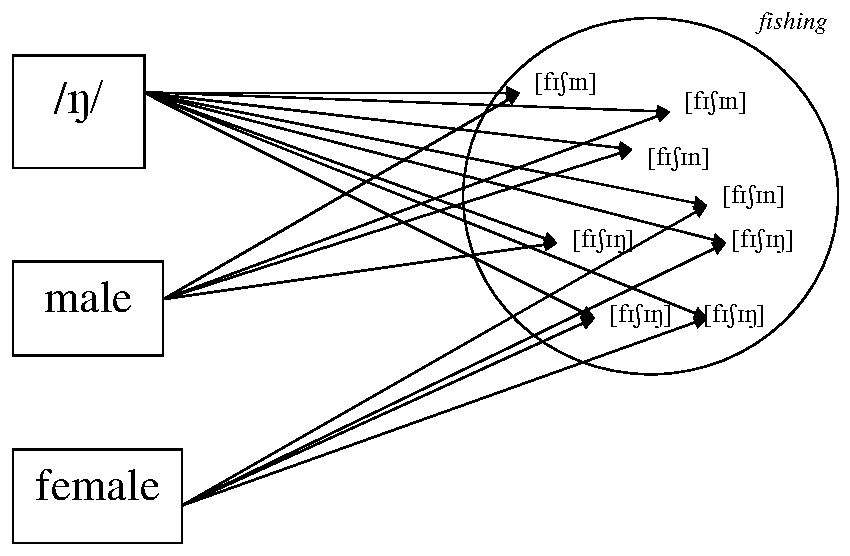
\includegraphics[width=.95\textwidth]{images/s90cr.pdf} %cropped version
	\caption{Sketch of \isi{exemplar model} based on results from \citet{trudgill1972} with distributions of remembered exemplars of the word \textit{fishing}.  Each exemplar is indexed to a label for phonemic category ({/{\ng}/}) and speaker sex (male and female).} 	\label{fig:with-phoneme-social-labels}
	
\end{figure} 

In addition to linguistic contextual information, exemplars are indexed to a myriad of other factors that are stored at the time of the utterance.  These include the formality of the situation and the social characteristics of the person who produced the utterance \citep{johnson1997,foulkesanddocherty2006}.  Again, \isi{salience} plays a role. Non-linguistic information is only stored if it was available at the time of the utterance and if it may be important to the perceiver \citep[147]{johnson1997}.  A sketch of this indexation is shown in \figref{fig:with-phoneme-social-labels} for an \isi{exemplar cloud} of the word \textit{fishing} within the context of \citegen{trudgill1972} finding that females were more likely to realise word final {/{\ng}/} as the velar nasal {[{\ng}]} whereas males were more likely to realise it as the alveolar nasal {[n]}.  Exemplars representing encountered utterances produced by males and females are indexed both to the phoneme level (e.g., {/{\ng}/}) and to characteristics of the speaker who produced the utterance (e.g., male).  


During production, the final realisation is a result of averaging over an entire region of an \isi{exemplar cloud}. There is not a one-to-one mapping of activated exemplar to the token that is ultimately perceived or produced \citep{pierrehumbert2001}.  This is in contrast to some presentations of exemplar models where a one-to-one mapping is assumed \citep{griffithsetal2007}.  Exemplars which have been activated recently and those which are activated frequently carry the highest weight values, resulting in a bias in production toward variants resembling these exemplars.  As with \isi{perception}, non-linguistic information indexed to the exemplars can bias which variants are produced.  After storage, exemplars immediately begin to decay and frequent \isi{activation} slows decay.  This \isi{activation} can occur through encountering an acoustically similar utterance. 

The region of an \isi{exemplar cloud} that is activated during production may be selected as a result of its indexation to social factors with which the speaker identifies.  Additionally, social characteristics of an addressee activate social exemplars, thereby biasing production toward the speech of that addressee in ways that depend on the speaker's attitudes toward the interlocutor \citep{drageretal2010,babel2012}.  This prediction is consistent with the well-known effects of audience design and speech accommodation \citep{bell1984,gilesetal1991,oprah1999}.

During \isi{perception}, exemplars are activated to varying levels depending on their similarity to the incoming utterance.  If incoming social information closely matches a previously stored social exemplar, the linguistic exemplar indexed to the social information will receive partial \isi{activation}.  These partially-activated exemplars reach full \isi{activation} faster than acoustically similar exemplars that are not indexed to a relevant social exemplar, resulting in a bias in \isi{perception} depending on the perceived social characteristics of the speaker \citep{strandjohnson1996,niedzielski1999,haywarrendrager2006}.   
 
Thus, exemplar-based models such as these predict a bias in both production and \isi{perception} toward socially relevant exemplars. Additionally, because diffe\-rent words with the same wordform are indexed to different \isi{lemma}-specific phonetic information, exemplar models predict that (1) there can be \isi{lemma}-conditioned phonetic variation in production that patterns according to exposure (a speaker's realisations will resemble those of other speakers with whom they regularly interact) and (2) individuals can use phonetic information based on trends in production to identify a \isi{lemma} during speech \isi{perception}.  And because exemplars are stored complete with acoustically-detailed information, it predicts that trends in production can be phonetically gradient and that individuals will be sensitive to acoustically-detailed information during the \isi{perception} of speech.

It is important to keep in mind that the mental representations reflect what was perceived, not what was produced or, even, what could potentially have been perceived.  This means that a number of factors, including attention, influence the form of the representation \citep{foulkeshay2015}.  

In many cases, exemplar-based models and \isi{Bayesian}-based models behave si\-milarly.	 \citet{pierrehumbert2002} states that an \isi{exemplar model} of speech production and \isi{perception} should be viewed as

\begin{quote}

a logical schema rather than taking it as a literal picture of activity in the brain.  Any model which stores implicit and incrementally updatable frequency distributions over a cognitive map will show similar behaviour; it is not important that all percepts are individuated as separate memories in the long term. \citep[113]{pierrehumbert2002}

\end{quote}

\noindent Even if episodic traces of acoustically-rich utterances are not stored, each utte\-rance could update the system in such a way that probabilities (with their base in frequency distributions) could be stored.  However, as evidenced by the work in the previous two chapters, this needs to include probabilities of very detailed, acoustically-rich information as well as very rich social information.

	
In conceptualising this logical schema, it may help to view different modes of representation for different levels of the grammar.  Rich phonetic detail of specific episodes may be stored and may influence both production and \isi{perception}, and probabilities may also be abstracted and stored, influencing the production and \isi{perception} of higher-level processes such as those involving syntactic information.  For example, a \isi{Bayesian}-based model could account for the effect of surrounding contextual information on \isi{lemma} identification in Experiment 1 and an exemplar-based model could account for the \isi{lemma}-conditioned phone\-tically gradient trends observed in production and the sensitivity to these trends observed in \isi{perception}. 


\section{Indexation of social information}\label{sec:richmodel}

In current exemplar-based models, such as those described by \citet{johnson1997} and \citet{haywarrendrager2010}, the representation of social information that is indexed to acoustically-rich exemplars is consistent with variationist work from the First and Second Waves of variation studies, where phonetic variables are treated as indexed directly to social categories. These categories can be broad, as in the sketch in \figref{fig:with-phoneme-social-labels}, or can be locally constructed.  

However, the representation of social information is much richer than this indexation would suggest.  In this section, I step through how, in the construction of social personae, the adoption and rejection of linguistic and non-linguistic features might be understood within an exemplar-based \isi{hybrid model}.

Work in the \isi{Third Wave} treats linguistic variables as directly indexed to style.  Style is complex; it is comprised of socially-meaningful components that can shift in meaning depending on other components indexed to the style.  From situation to situation, the style of a single speaker can shift, sometimes subtly, sometimes dramatically.  

A speaker's \isi{stance} can serve to create that speaker's style.  For example, if a speaker views themselves as ``different'' from the norm, they create their indivi\-dual style through the expression of this \isi{stance}.  At SGH, goths and geeks created different styles from one another but because their \isi{stance} was in opposition to a third group (e.g., \isi{The PCs} or the CR girls as a whole), some of their styles could have components that resembled each other (e.g., patterns of \isi{/k/} realisation in quotative and discourse particle \textit{like}).

\citet{mendozadentonetal2003} state that a usage-based probabilistic model is

\begin{quote}
entirely compatible with a view of the social world that relies on gradually built up social categories that emerge from experiences that surround individuals as social actors. \citep[136]{mendozadentonetal2003}
\end{quote}

\noindent Yet, no one has spelled out how stylistic variation occurs within the context of a probabilistic linguistic model.  One challenge that arises when trying to do so is that potential stylistic components not only come to be imbued with \isi{social meaning} based on the presence of an item, activity, or characteristic but also from the absence of wearing certain items or from not taking part in certain activities.  For example, Santra (\isi{The Goths}, NCR) wore black clothes and the colour of the clothes was meaningful in that it helped to construct her social persona.  But also meaningful was that Santra did not wear mini skirts or bright colours.  One day when she wore a green shirt, someone commented that they had never seen her wear a bright colour before.  Santra confessed that she didn't feel like herself and was looking forward to going home so that she could change clothes.  Refraining from participating in certain activities (e.g., wearing bright colours), both linguistic and non-linguistic, can itself be socially meaningful and helps to contribute to a speaker's style.  But if exemplar clouds are based on previously encountered occurrences, how does the lack of a characteristic or item of clothing become a stylistic component?  The model presented here addresses this through the indexation of a speaker's style to different parts of multidimensional stylistic features: the part of the distribution to which a speaker's style is indexed indicates the degree to which that component is adopted in the construction of her style.  Both identification and avoidance can occur through comparing how different styles index different parts of \isi{multidimensional representations} of stylistic components.

In \figref{fig:SketchTwoStyles2}, I present a sketch of Santra's (\isi{The Goths}, NCR) style and Betty's (\isi{The Sporty Girls}', CR) style within the context of an \isi{exemplar model} of speech production and \isi{perception}.  Of course, a speaker's style is multidimensional and shifts depending on the situation.  A speaker's shifting style may not be the overt abstraction implied by the sketch in \figref{fig:SketchTwoStyles2}.  Instead, components may be indexed to a representation of the speaker and that speaker's style could arise with particular patterns of \isi{activation} over the components.  This could account for how styles shift in ways that are sometimes subtle and sometimes dramatic.  For simplicity, the styles modelled here represent the general styles that were consistently observed for the girls within the context of the school.  Each of the components is based on their own cloud of exemplars, where the stored exemplars are representations of previous encounters with each of the girls.  

\begin{figure}
	\centering
		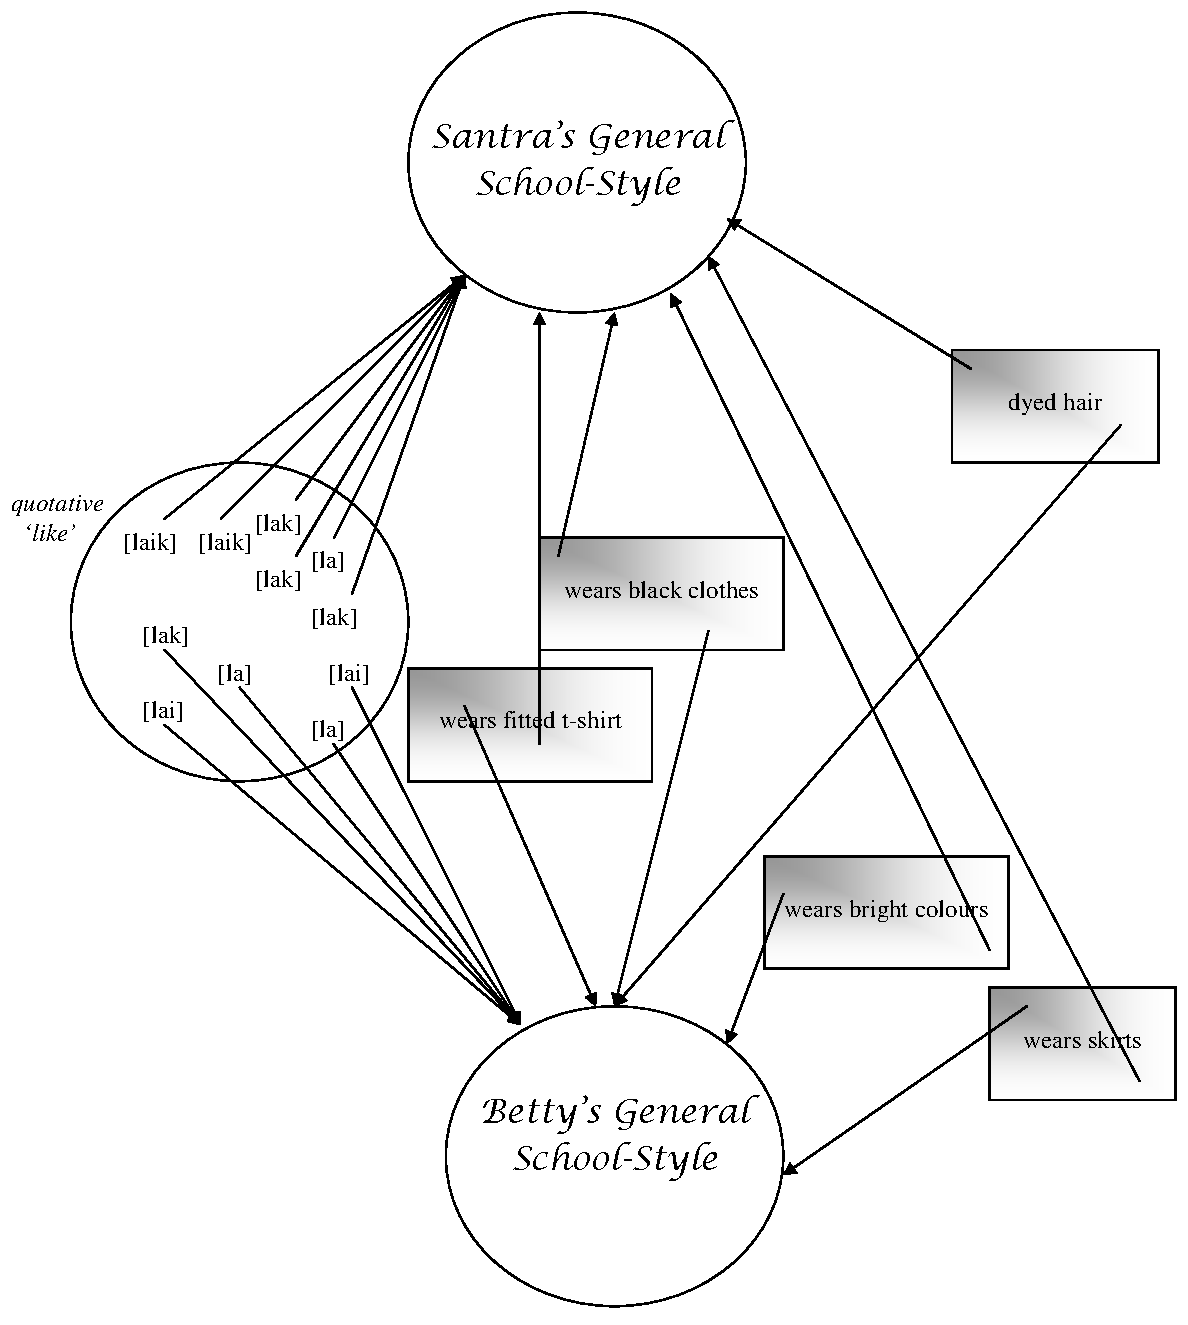
\includegraphics[width = \textwidth]{images/s2scr.pdf} %replaced by cropped img
	\caption{Sketch of two speakers' styles and their linguistic and non-linguistic components.  The portion of the shaded box that is indexed reflects the degree to which an individual adopts or rejects that characteristic when constructing a given style.}
	\label{fig:SketchTwoStyles2}
\end{figure}



In order for the lack of an item to become socially meaningful, comparisons must be made between potential stylistic components observed in a social arena.  Different individuals will vary probabilistically in how they are indexed to these components and the components themselves become more socially meaningful the further apart the sections are that the different styles index.  In \figref{fig:SketchTwoStyles2}, this is displayed through indexing different regions of multidimensional components; different parts of the \isi{multidimensional representations} are indexed depending on the likelihood of a girl possessing that item or characteristic.  Here, I have treated the horizontal plane within each shaded box as frequency across time (e.g., some girls were more likely to wear a skirt than others) and the vertical plane as another dimension at a given point in time, such as the number of items worn in that colour or the length of a skirt when worn.  For example, `wears black' is labelled as a stylistic component and the styles of different girls are indexed to different parts of this abstract representation depending both on how often they wear black and, when wearing black, how much of their clothing is black.  The style represented for Betty is indexed to the whiter region of the box, indicating that she wears black less than half of the time and, when even wearing black, does not wear many items that are black.  This indexation reflects the probability that a single speaker will adopt one of these stylistic components, thereby constructing their personal style.  Indexation can occur not only through the storage of exemplars based on experience with an individual, but through the comparison of that individual with others.  

Not all items or characteristics that could potentially be components of an individual's style become imbued with \isi{social meaning}.  For example, both Santra and Betty wore tight-fitting t-shirts.  Donning this type of shirt was not particularly meaningful in differentiating their different styles; this is reflected in their inde\-xation to a similar space within this potential component.  However, the colour of the top was potentially meaningful: Betty's might be blue or black depending on the day whereas Santra's was almost certainly black.  

That indexation of stylistic components relies on comparisons also ensures that the lack of an item or characteristic is meaningful only within the context of a given social arena.  This is desirable because traits that are completely absent from the reality of the social arena do not meaningfully affect an individual's style.  For example, that Santra did not wear a tiara was not socially meaningful because none of the girls wore tiaras to school.  

Linguistic variation, like the variation found among other stylistic components, can be converged upon or diverged from depending on both the speaker's attitudes toward an individual and how similar they believe they are to the indivi\-dual.  As with other stylistic components, indexation may occur not only between a speaker's style and a phonetically-rich exemplar representing an utterance produced by that speaker, but also through the absence of producing a particular variant.  A sketch of this relationship is shown in \figref{fig:SketchStylesLing}. While the sketch shows only two dimensions, the model is not limited in this way. Furthermore, it is important to note that speakers can shift their indexations between different parts of the mutlidimensional space and that this shift can occur throughout an interaction.

\begin{figure}
	\centering
		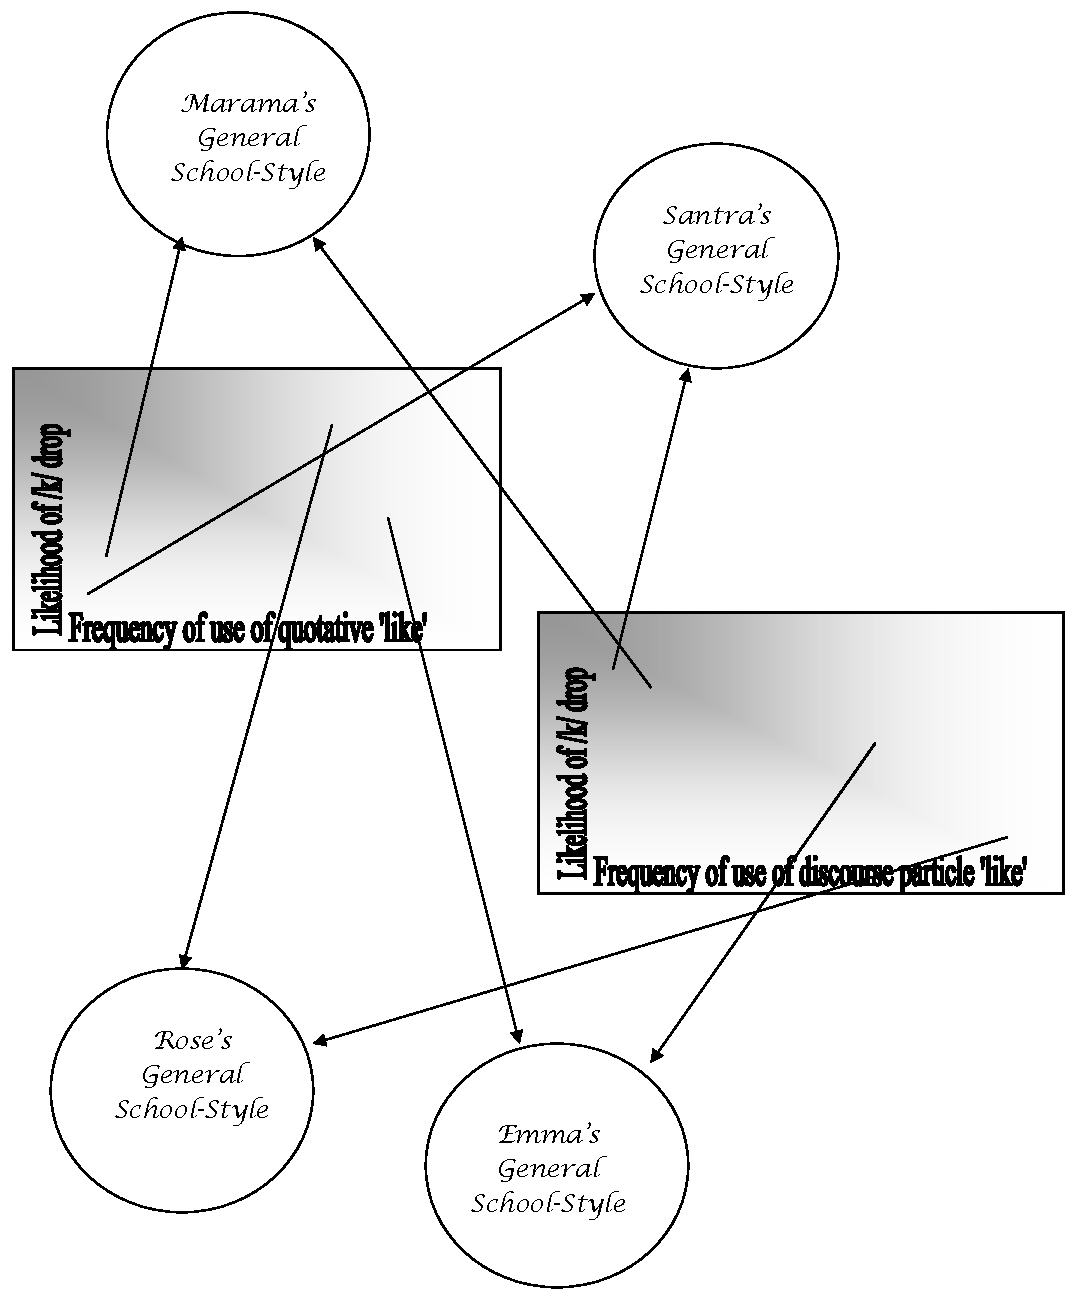
\includegraphics[width=\textwidth]{images/sslcr.pdf} % replaced SketchStylesLing.pdf with cropped version
% 	%\documentclass[a4paper]{article}
%\usepackage{pgfplots}
%
%\begin{document}

\tikzset{every mark/.append style={scale=1.5}}
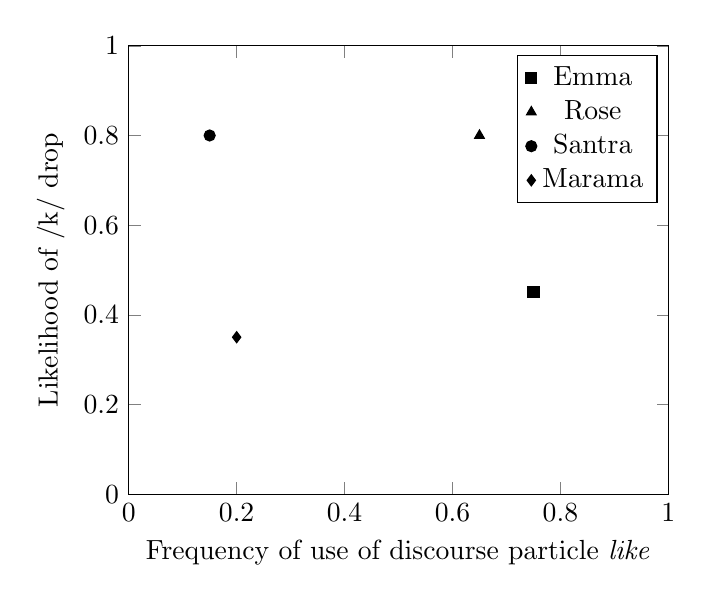
\begin{tikzpicture}
\begin{axis}[xmin=0,xmax=1,ymin=0,ymax=1, scatter/classes={e={mark=square*},r={mark=triangle*},s={mark=*,draw=black}, m={mark=diamond*}}, xlabel={Frequency of use of discourse particle \textit{like}},ylabel={Likelihood of /k/ drop}]
\addplot[scatter,only marks, scatter src=explicit symbolic] coordinates{
	(0.75,0.45) [e]
	(0.65,0.80) [r]
	(0.15,0.80) [s]
	(0.20,0.35) [m]
	};
\legend{Emma, Rose, Santra, Marama}
\end{axis}
\end{tikzpicture}
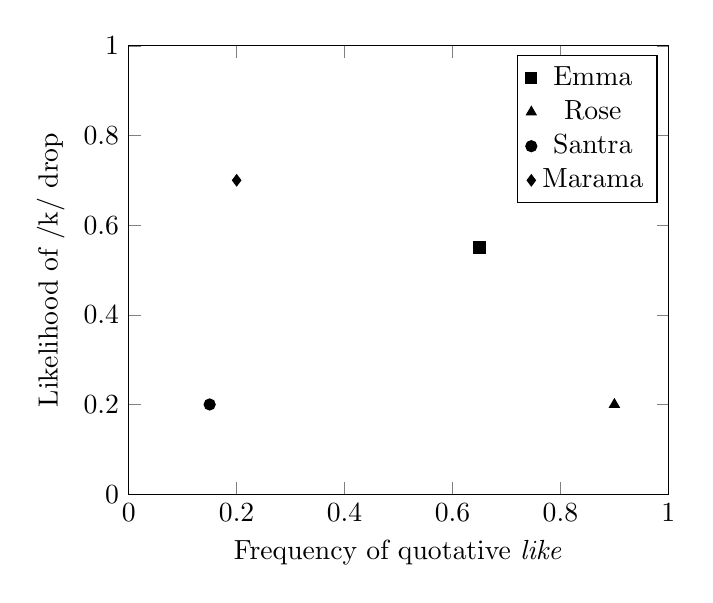
\begin{tikzpicture}
\begin{axis}[xmin=0,xmax=1,ymin=0,ymax=1, scatter/classes={e={mark=square*},r={mark=triangle*},s={mark=*,draw=black}, m={mark=diamond*}}, xlabel={Frequency of quotative \textit{like}},ylabel={Likelihood of /k/ drop}]
\addplot[scatter,only marks, scatter src=explicit symbolic] coordinates{
	(0.65,0.55) [e]
	(0.90,0.20) [r]
	(0.15,0.20) [s]
	(0.20,0.70) [m]
	};
\legend{Emma, Rose, Santra, Marama}
\end{axis}
\end{tikzpicture}
%\end{document}
	\caption{Sketch of indexation between multidimensional linguistic components and speakers' styles. For simplicity, only two dimensions are shown: frequency of using quoative \textit{like} is shown on the x-axis and the likelihood of dropping the \isi{/k/} is on the y-axis.}
	\label{fig:SketchStylesLing}
\end{figure}


As with non-linguistic elements, linguistic components of style are multidimensional, with different styles indexed to different parts of the distribution.  The dimensions represented in \figref{fig:SketchStylesLing} are frequency of use (along the horizontal plane) and the likelihood of realising the \isi{/k/} in any given token (along the vertical plane). For example, Marama's General School-Style is indexed to the portion of the distribution of quotative \textit{like} where there is a relatively low likelihood of dropping the \isi{/k/} in addition to a lower frequency of use of the quotative when compared with many of her peers.  In contrast, her School-Style is indexed to the portion of the distribution of discourse particle \textit{like} where there is a high likelihood of dropping the \isi{/k/} and a low frequency of using the discourse particle relative to other girls at the school.  Of course, other dimensions would include other information, such as the duration of a segment and the frequency bands of the formants.  Such indexation to \isi{multidimensional representations} of linguistic variables predicts that \isi{identity} construction will result in convergence among speakers constructing similar styles to one another.  Because distributions of these indices can be compared across different speakers, it also predicts divergence by individuals wishing to differentiate themselves from a particular style; indexation to the multidimensional space can be manipulated through comparison of stored indices of other speakers' styles to the space.  A speaker can index a space that is void of exemplars and can do so in relation to the observed behaviour of the other speakers.

  
These patterns of \isi{activation} over the multitude of components that comprise a style can explain how vowel shifts can occur within an exemplar-based \isi{hybrid model}.  In \citegen{pierrehumbert2001} model, vowel shifts could only be driven by a speaker producing variants outside the realm of previously stored exemplars as a result of random noise; there is no socially-driven motivation for vowel shifts built in to the model.  However, it is highly unlikely that vowel shifts result entirely from random noise: individuals who lead vowel shifts are the same individuals who lead other stylistic changes \citep{labov2001}.  For example, elementary school girls who produce the most extreme phonetic variants are the same individuals who begin wearing nail polish or lacy underwear \citep{eckert1996nailpolish}; they are the individuals who first adopt the most extreme components of styles from the heterosexual marketplace in the construction of their \isi{identity} within an emerging peer social order.  The model presented here, which combines acoustically-detailed episodic memories with multi-dimensional abstractions of the acoustic space, a\-llows speakers to index these spaces that are potentially void of acoustically-rich exemplars.  This indexation can have a direct effect on the variants produced; speakers constructing personae that are extreme within the context of a social arena can produce variants that are extreme in comparison to other speakers in that arena.  Linguistic variation is a stylistic resource and the manner in which it is stored must allow for the construction of a speaker's \isi{identity}.
%see page 360-364 for Labov's work


\section{Conclusion}

In this chapter, I discussed two \isi{probabilistic models} of language use and I described how they can account for the results presented in the preceding two chapters.  The most comprehensive model may be some combination of these, incorporating both stored exemplars of utterances complete with acoustic detail and abstracted probabilities of phrase structures.  In a model where clouds of phonetically-rich exemplars contribute to abstractions of multidimensional stylistic components, it is possible to account for phonetic variation that patterns according to stylistic choices made by the speaker.  



%\newpage
%\thispagestyle{empty}
%\mbox{}
\chapter{Looking forward}
\label{ch:concl}


\epigraph{They may change their roles, their styles of acting, even the dramas in which they play; but -- as Shakespeare himself of course remarked -- they are always performing.}{\citep[35--36]{geertz1973}} 

\noindent Individuals manipulate linguistic variables in the construction of their identities, displaying their \isi{communicative competence} within the context of the social world in which they participate.  Probabilistic models provide a means of uniting social and linguistic theory and this unification has been a driving force behind the methods and analyses used for this book.  

In Chapters \ref{ch:ethnography} and \ref{ch:prod}, the analysis concerned both the individual girls' styles constructed within the school and the components that make up this style, with a particular emphasis on stylistic phonetic variation of different words.  The results presented in \chapref{ch:perc} display how individuals can use phonetic information when identifying a word, even when the words are identical at the phonological level, and that listeners can identify the function of a word and, to some extent, attribute social characteristics to the speakers based on phonetic information in the stimulus.  In \chapref{ch:disc}, I presented a probabilistic model of speech production, \isi{perception} and \isi{identity} construction in which multidimensional stylistic components are indexed to a speaker's style.  My hope is that this model will serve as a stepping stone from which to explore the integration of social and linguistic theory in future work.  

In the remainder of this chapter, I present one possible avenue of inquiry that I believe will aid our understanding of the way in which mental representations of sociolinguistic variables are accessed during the production and \isi{perception} of speech, ultimately leading to a better understanding of human cognition.

 

\section{Speakers as style-creators}

\noindent Variationist sociolinguists who examine style are increasingly turning their attention to the individual \citep{eckert1996,eckert2011,podesva2011}.  This is important because individuals create \isi{stance} and style during interaction and, therefore, \isi{stance} and style need to be examined as processes that emerge in context (see e.g., \citet{coupland2007,kiesling2009,rampton2013}. For example, \citet[110--115]{bucholtz2010} demonstrates how quotative variants used by \isi{high school} students were influenced by a combination of the speaker's \isi{stance} and their social group: preppy students were more likely to use \textit{be all} when taking a neutral \isi{stance}, whereas non-preppy students were more likely to use \textit{be all} when taking a non-neutral \isi{stance}.  In her study on phonetic realisations of bilingual children, \citet{khattab2013} shows how the children sometimes adopt phonetic features from their parents' non-native English accents to do social work, shifting between native-like and non-native-like realisations in socially-meaningful ways.  This work demonstrates how a single linguistic variant can be used to achieve multiple (and, in some cases, quite different) social goals. Work by Schilling-Estes demonstrates how speakers' sociolinguistic variants shift as a function of both their stances and the variants produced by their interlocutors \citep{schillingestes2004}. Finally, \citet{kirtley-diss} demonstrates how individual speakers use different phonetic variants for social purposes, many of which can be perceived both as being consistent with a particular trait (e.g., masculinity) and as highlighting different aspects of that trait (e.g., the many different ways of being masculine and of doing masculinity).  

When examining \isi{stance}-taking and style-making by individuals, it is important to keep in mind the \isi{social groups} to which these speakers orient.  It is believed that linguistic forms are directly indexed to stances and that the linguistic forms become indirectly indexed with \isi{social groups} who regularly take or are believed to take those stances \citep{bucholtz2009,dubois2007}. Alternatively, it seems plausible that speakers wishing to construct a certain style or take a particular \isi{stance} may do so by drawing on pre-existing indexations between (or ideologies around) linguistic forms and \isi{social groups}.  The reality is likely a combination of these, where a variable that is ideologically linked with a group is adopted to take stances that are habitually taken or are associated with that group, and that those variables can then become indexed with new social categories via the stances they enact.

In this book, I have examined \isi{stance} and style across \isi{social groups} and, though I recognise that stances and styles are not stagnant, I have largely treated them this way in my analysis.  I have done this due to time restrictions and because I believe that variation in interaction has the most explanatory power when situated within a larger context for that variation.  During stancetaking, speakers do not select linguistic variants out of the blue: the variants are indexed to social meanings (social meanings that can be multiple and complex) through ideologies around what kinds of people produce what variants.  Therefore, understanding the ideologies and the ways in which variables pattern across \isi{social groups} is important for understanding how the variables are manipulated in the construction of \isi{stance} and style in interaction.

With this in mind, in \citet{dragerinpress-DPVC} I revisited the SGH data to gain insight into how the girls manipulated realisations of quotative and discourse particle \textit{like} when taking various stances in interaction.  The phonetic analysis was restricted to the tokens analysed for Chapter \ref{ch:prod} of this book and focused on tokens from narratives that included references to other groups or individuals.  The speakers' stances toward the referents were identified (removing those that were ambiguous or unknown) and the tokens were compared within the speech of a single individual.  
 

Three trends emerged from this analysis that are especially noteworthy.  The first is that, for some speakers, their interactional stances appear to be related to the frequency with which they produce discourse particle \textit{like}.  For example, \isi{The Goths} (a non-Common Room group) frequently produced discourse particle \textit{like}, but they did not produce any tokens when making claims about how they were different from other ``normal'' girls at SGH.  Because the discursive functions of \textit{like} are highly associated with Common Room groups (and \isi{The PCs} in particular), the absence of discourse particle \textit{like} in these segments helps to highlight that \isi{The Goths} are different from the Common Room groups.  The second trend that emerged is that some speakers' realisations of discourse \textit{like} contained little phonetic variation.\footnote{I noticed this during the analysis presented in Chapter \ref{ch:prod} but, at the time, failed to comment on the importance of it for the construction of \isi{social meaning}.}  The only speaker to produce both the quotative and discourse particle as [laik] for all of the analysed tokens was Mariah (\isi{The Geeks}), who not only consistently realised the \isi{/k/} but produced it with a long release.  Mariah generally produced clear speech, including the release of other stops, such as /t/.  Articulation of stop releases is ideologically associated with intelligence, a trait that was valued by members of \isi{The Geeks}, and strong releases have also been found to be used by geek girls in the United States \citep[125]{bucholtz1998}. Thus, Mariah's realisations of \textit{like} help to construct her personal style. 
\largerpage[-1]

A third trend that emerged concerns the realisations of quotative \textit{like} in which the speakers' evaluations of the referents differ, resulting in a change in \isi{footing} \citep{goffman1981}.  The speech of two girls, Patricia and Kanani (both from The Sporty Group, a CR group), is especially revealing.  Patricia and Kanani were the two CR girls whose patterns of realisations of \textit{like} were most similar to the \isi{NCR girls} (see  \sectref{theindividual}).  In Chapter \ref{ch:prod}, I attributed this to their particular social histories and backgrounds: Kanani was formerly a member of a NCR group (so may still have had some NCR group speech characteristics) and Patricia's closest friends went to other schools (and her friends' patterns of realisations of \textit{like} are unknown).  However, after examining how \textit{like} was used in interaction, I now believe Patricia and Kanani were doing something much more complicated and socially-meaningful: they seem to have been manipulating their realisations of quotative \textit{like} as a part of their stancetaking toward the person whose speech they were reporting.  An example from Kanani's speech is shown in Example \ref{ex:kanani-interaction}.   


\sent{
1 Kanani: 		I remember this chick rung up (.) for my brother 

2	\hspace{3em} and um (.)

3 \hspace{3em} hh she's like$_1$ ``hi is Kimo there please''

4 \hspace{3em} I'm like$_2$ ``oh he's in the toilet at the moment'' (.)

5 \hspace{3em} she's like$_3$ (.) ``thanks''

6  \hspace{3em} 					$<$laughter$>$

7 Rose: \hspace{1em} 		I would've been like ``oh actually he's just 
	
	\hspace{5em} [really constipated'' ]

8 KD: \hspace{2em} 	[``he's doing poos''  ]

9 Rose: \hspace{1em}		yeah

10 \hspace{3em}        $<$laughter:$>$

11 Kanani: 	and then my brother came and got the phone 

12 \hspace{3em} and he's like$_4$ $<$raises eyebrows$>$ 

13 \hspace{3em} he went off the phone he's like$_5$ ``what a dick''
 
}\label{ex:kanani-interaction}

\noindent In this example, Kanani is telling a story about her popular and attractive brother, Kimo, receiving a phone call from a woman, a ``chick'' (line 1) who she had never met.  Kanani was very close with her brother - she was very family-oriented in general - and didn't necessarily approve of the woman who called.  Within the context of the conversation, Kanani positions herself as family-oriented and down-to-earth, and the woman who rings up as coquettish and silly.  These positionings align with the realisations of quotative \textit{like}: when preceding her own or her brother's speech, the quotative is realised with a less diphthongal vowel and no \isi{/k/} (the ``CR realisation''), whereas when introducing the speech of the woman on the phone, the vowel is diphthongal and the \isi{/k/} is present (the ``NCR realisation''). These trends do not appear to result from phonological environment or \isi{speech rate}: like$_5$ (line 13) is followed by /w/, an environment which promotes the realisation of \isi{/k/} in quotative \textit{like}, but the \isi{/k/} is not realised.  Likewise, given the relatively quick \isi{speech rate} in like$_1$ (line 3), we might expect a monophthongal vowel but, in fact, the vowel is diphthongal.

\begin{table}[htbp]
\caption{Phonetic realisations of tokens of \textit{like} found in Example (\ref{ex:kanani-interaction}), adapted from Table 5 in \citet{drager2016}.  The Euclidean di\isi{stance} (EucD) is shown in Bark and \isi{speech rate} is syllables per second in the IP surrounding the token but does not include the token itself.}	
	\label{tab:kanani-interaction}
	 \begin{center}
		\begin{tabular}{llrcr}\lsptoprule
	
   token & referent & EucD & \isi{/k/} present & syllables/sec\\
  \midrule
like$_1$ & woman & 2.24 & y & 4.88 \\
like$_2$ & Kanani & 1.36 & n & 6.47 \\
like$_3$ & woman & 2.53 & y & 2.78 \\
like$_4$ & brother & 0.31 & n & 5.26 \\
like$_5$ & brother & 1.53 & n & 4.08 \\

\lspbottomrule
		\end{tabular}
	
	\end{center}
\end{table} 

In other words, when reporting the speech of someone who she aligned with, Kanani produces quotative \textit{like} with a monophthongal vowel and non-realised \isi{/k/} (the CR realisation), whereas she produces it with a diphthongal vowel and [k] when reporting the speech of someone who she does not know or respect.  This suggests that Kanani does not have imperfect acquisition of the variable as a result of changing from a non-Common Room to a Common Room group; instead, she demonstrates a sophisticated knowledge of both systems and appears to use it as a narrative device. In fact, it is possible that her social history provided her with greater (unconscious) control of the variable as a result of having greater exposure.

Some other girls (e.g., Meredith, Isabelle, and Patricia) demonstrate analogous trends, with appropriate realisations for their group (CR or NCR).  For other speakers, a trend is less clear (or is non-existent as in the case of Mariah) and the analysis is complicated by ambiguous or unknown stances.  Additionally, other factors such as \isi{speech rate} and \isi{pitch} that are linked with the phonetic variables of interest are not controlled for in this type of analysis, which limits the data one can reliably use to examine variation of this type.\footnote{Variation in \isi{speech rate} and \isi{pitch} can, of course, be socially meaningful.  When they are, variation in related phonetic variables may in fact be an epiphenomenon.}  

In my estimation, the finding that phonetic realisations of quotative \textit{like} are conditioned by interactional \isi{stance} is more suggestive than conclusive due to the relatively small number of speakers and data points that demonstrate the trend. But, given the fact that other researchers have demonstrated that the form of the quotative (e.g., \textit{be like} vs. \textit{be all}) varies by \isi{stance}, we might actually expect that the realisations of these highly salient words would vary, particularly when - like in these data - \textit{be like} so strongly dominates the quotative system of all of the speakers.  It is worth noting that the variation in the realisation of discourse \textit{like} does not negate the quantitative findings presented in this book.  Because only some individuals seem to vary their realisations of quotative \textit{like} in this way and because the girls so frequently voice their own or their friend's speech, the trends reported in Chapter \ref{ch:prod} do seem to be the most frequent realisations.  In fact, the distinction between CR and NCR realisations is needed to interpret the \isi{stance}-based variation reported by \citet{dragerinpress-DPVC}.  Taken together, the work suggests that speakers can use probabilistic patterns of sociolinguistic variables (including those tied with locally-constructed social categories) to help take stances during the course of an interaction, but much more work along these lines is needed.




%\section{Listeners as individuals}
%In contrast with the growing amount of work that focuses on the individual in production, there is very little work that focuses on how individual listeners' \isi{perception} may differ and what factors might influence this variation.  While such variation is known to exist, it is generally something that experimentalists try to control statistically in their data rather than study in its own right.  When experimentalists report on variation across different listeners or voices, they focus not on individuals so much as groups of individuals.  For example, in their investigation of learning sociophonetic patterns, Docherty et al. (2013) found that some listeners learned a probabilistic pattern categorically, whereas others learned it probabilistically or, even, not at all.  Others have focused on personality traits (cite) or other social characteristics \ref{dragerunderrev} (cite more) or other kinds of traits such as the individual's degree of autism \citep{yu2010}.  

%One variable that I'm particularly interested in is attention.  Individuals have some degree of control over attention and may choose to attend to something other than the experimental task.  Relevance (define) and \isi{salience} (the degree to which something stands out) also influence attention.  For example, if an item is larger or louder than the surrounding items, it has a higher likelihood of drawing the perceiver's attention. And it is clear that varying attention is a source of variation in individual's \isi{perception} of sociolinguistic variables (see the discussion in Drager and Kirtley (in press)). \nocite{dragerkirtley-salience} 

%Likewise, there is little work that focuses on variation across different voices.  Campbell-Kibler (2007) demonstrates how person \isi{perception} varies depending on the voice, attributing the differences to other characteristics that are also attributed to the voices.  Similar results have also been found by other scholars (e.g., Drager, Schutz, Chik, Hardeman, and Jih 2012). Early \isi{perception} work by Labov [find and update] demonstrates how individuals perceive speech when listening to their own voices or a voice of a confederate, but this is not commonly done.  In the interest of 
%\nocite{campbellkibler2007}

%As reported in Chapter \ref{ch:perc}, there were low accuracy rates overall at accurately identifying the voices.  The girls did not even accurately identify themselves; of the four listeners whose voices were used as stimuli, Tracy was the only one to accurately identify herself in this task.

%The most popular girl whose voice was used in Experiment 3, Tracy (a PC), was also the speaker who was most commonly identified; of the 27 girls who tried to identify any speaker, 13 individual girls (including Tracy) accurately identified her (compared to the 9 times that the next most commonly identified girl was identified).  That Tracy was the most accurately recognised is not particularly surprising given the prominent role she played in the school. [what are the implications of this for storage and retrieval?]

%- we observe effects in sociophonetic \isi{perception} b/c of correlations across groups (walker & hay 2011 etc) that exist due to a combination of exposure and ideologies


%Of the seven remaining voices, four of them were accurately identified at roughly similar levels: Rose - 9 times, Sarah - 9 times, Isabelle - 8 times, and Meredith - 7 times.  Rose (Relaxed Group, CR) was only accurately identified by other CR girls, all of whom she has some degree of contact with.  Likewise, Meredith (\isi{The Goths}, NCR) was only identified by \isi{NCR girls}.  




%\section{Linking the individual with the community}
%``...even within the same speech community individuals will differ in their exposure to patters of phonetic variability'' (Docherty and Foulkes 2014: 48).
%``It remains unclear [in exemplar-based models] how shared abstract representations of phonological patterning and lexical referents are derived from the variable experiences that individuals have...'' (Docherty and Foulkes 2014: 48)
%what falls out probabilistically, what doesn't
%ideologies and attitudes

%- how are stereotypes and ideologies represented?


\section{Concluding remarks}


The findings presented in this book demonstrate the benefits of combining qualitative and quantitative analysis and of examining variation in both production and \isi{perception}.  While I do not advocate abandoning traditional variationist description by any means, I do believe that inroads will be made by variationists who choose to explore multiple avenues of inquiry.  In continuing the progression of social theory through the investigation of linguistic variation, sociolinguistics will benefit from increased focus on variation in speech \isi{perception} in addition to production, using computational models to explore sociolinguistic assumptions and predictions, examining the behaviour of individuals within a single interaction, and using insights from other areas of empirical linguistics such as \isi{laboratory phonology}.  Additionally, \isi{laboratory phonology} will benefit from incorporating more socially-informed data and analyses, not only by examining speakers' and listeners' social characteristics but moving toward a more nuanced treatment of socially-conditioned variation that includes a focus on the individual and the individual's goals in interaction. As sociolinguists have long argued, the division of language into the social and the non-social is artificial; the time is ripe for social theory and linguistic theory to be examined together within the context of unified models of language use.

%%%%%%%%%%%%%%%%%%%%%%%%%%%%%%%%%%%%%%%%%%%%%%%%%%%%
%%%                                              %%%
%%%             Backmatter                       %%%
%%%                                              %%%
%%%%%%%%%%%%%%%%%%%%%%%%%%%%%%%%%%%%%%%%%%%%%%%%%%%%
\appendix
%\documentclass[12pt]{article}
%\usepackage{harvard}
%\usepackage{fullpage}
%\usepackage{graphicx}
%\usepackage{times}
%\usepackage[safe]{tipa}
%\usepackage{tipa}
%\usepackage[section]{placeins}
%\bibliographystyle{kluwer}

%\renewcommand{\baselinestretch}{1.5} 

%\begin{document}
%\date{} 
\chapter{Measures of familiarity}\label{app:socialgroups}
%\maketitle
\noindent This appendix provides the names of girls in each group.  Also provided is a number indicating how well I felt I knew each girl, where 5 is highly familiar and 1 is knew by name and sight only. 

Girls who took part in the perception experiment and whose speech was analysed for the production study are marked with two crosses (++).  Girls who only took part in the perception experiment are marked with a single cross (+).
%-How to define `how close with me'?  Scale of 1-5, where 1 is knew by sight and overhearing but little direct interaction, 2 is only talking with a few times, 3 is talk regularly but still feel like I don't know particularly well, 4 is talk regularly and know quite well, 5 = she seeks me out for company, texts me, and wants to or does hang out outside of school


\section{CR Groups}

\subsection{The Sporty Girls}
\nopagebreak
\begin{table}[ht]
\caption{The Sporty Girls, by how central to group and how well I felt I knew them.}\label{append:Sporty}
	\centering
		\begin{tabular}{p{4cm}cr} \\
		\lsptoprule
		\multirow{2}{*}{\sc name} & \multicolumn{1}{p{2cm}}{\centering \sc centrality to group} & \multicolumn{1}{p{1.75cm}}{\centering \sc how close with me} \\
			\midrule
Naomi   & main & 3 \\
Stella  & main & 3 \\
Rachael & main & 3 \\
Elise   & core & 2 \\
Candice & core & 2 \\  
Patricia ++ & fringe & 3 \\ 
Ruby    & core &  2 \\   
Betty  ++  & fringe & 4 \\  
Kanani (previously of\\The Pasifika Group) ++  & fringe & 5 \\
   \lspbottomrule
		\end{tabular}
\end{table}

\pagebreak

\subsection {The PCs}
\nopagebreak
\begin{table}[ht]
\caption{The PCs, by how central to group and how well I felt I knew them.}\label{PCnames}
	\centering
		\begin{tabular}{lcr} \\
		\lsptoprule
		
			\multirow{2}{*}{\sc name} & \multicolumn{1}{p{2cm}}{\centering \sc centrality to group} & \multicolumn{1}{p{1.75cm}}{\centering \sc how close with me}  \\
			\midrule
			
			Joanna		&		main		&		2  \\
			June			&		core/main &  1 \\
			Tracy ++			&		core		&		4 \\
			Juliet ++	&   core		&		4 \\
			Emma ++		&		core		&		4 \\
			Kim				&		core		&		3 \\
			Pixie			&		core		&		3 \\
			Kendra		&		core		&		3 \\
			Daphne		&		core		&		3 \\
			Darby   	&		core		&		2 \\
			Marilyn 	&		core		&		2 \\
			Aurora		&		core		&		1 \\
			Zindri		&		core		&		1 \\
			Gabrielle	&		core		&		1 \\
			Minnie		&		core		&		1 \\
			Gina			&		fringe	&		2 \\
			Noelle		&		fringe	&		1 \\
			Amber   	&   fringe	&		1 \\
			Cleo			&		fringe	&		1 \\
			Katya			&		fringe	&		1 \\	
			
			   \lspbottomrule
		\end{tabular}
\end{table}


\pagebreak

\subsection{Trendy Alternatives}
\nopagebreak
\begin{table}[ht]
\caption{The Trendy Alternatives, by how central to group and how well I felt I knew them.}	\label{append:Alternatives}
	\centering
		\begin{tabular}{lcr} \\
		\lsptoprule
			\multirow{2}{*}{\sc name} & \multicolumn{1}{p{2cm}}{\centering \sc centrality to group} & \multicolumn{1}{p{1.75cm}}{\centering \sc how close with me}  \\
			\midrule
Justine ++ & main & 3 \\
Kelly & core & 4 \\
Clementine ++ & core & 3 \\
Jewel  & core & 3 \\
Carla  & core & 3 \\
Christina ++ & core & 3 \\
Felicity & core & 2 \\
Lily  & fringe & 5 \\
Pascal +  & fringe & 4 \\

   \lspbottomrule
		\end{tabular}
\end{table}

\subsection{Rochelle's Group}
\nopagebreak
\begin{table}[ht]
\caption{Rochelle's Group, by how central to group and how well I felt I knew them.}	\label{append:Drama}
	\centering
		\begin{tabular}{p{4cm}cr} \\
		\lsptoprule
			\multirow{2}{*}{\sc name} & \multicolumn{1}{p{2cm}}{\centering \sc centrality to group} & \multicolumn{1}{p{1.75cm}}{\centering \sc how close with me}  \\
		\midrule
		Rochelle ++ & main & 5 \\
		Camden   & main/core & 5 \\
		Chantelle & core & 2 \\
		Mindy     & core & 2 \\
		Lorna (also friends with The Relaxed Group)    & fringe & 2 \\
		   \lspbottomrule
	\end{tabular}
\end{table}


\pagebreak
\subsection {The BBs}
\nopagebreak
The original BBs in\-cluded Star, Ma\-di\-son, Ja\-clyn, Za\-ra, Gwen, and Pris\-cil\-la.  The other half of the merged group (originally referred to as Pam's group) included Pam, Odette, Glenda, Jane, Shannon, Annie, Brooke, Andrea, Natasha, Ursula, Denise, Laura, and Maya.  In Table \ref{BBnames}, names followed by an asterisk denote members of the subgroup usually referred to as the BBs.  The other girls were a part of what was originally referred to as Pam's Group.
\begin{table}[H]
\caption{The BBs, by how central to group and how well I felt I knew them.}	\label{BBnames}
	\centering
		\begin{tabular}{lcr}
		\lsptoprule
			\multirow{2}{*}{\sc name} & \multicolumn{1}{p{2cm}}{\centering \sc centrality to group} & \multicolumn{1}{p{1.75cm}}{\centering \sc how close with me}  \\
		\midrule
			
			Star * 		&		main	&		2 \\
			Madison *	&		main	&		3 \\
			Pam			&		main	&		3 \\
			Jaclyn *	&		core	&		3 \\
			Zara *	&		core	&		1 \\
			Priscilla * & core	&		1 \\
			Gwen *		&		fringe &	3 \\
			Glenda +	&		core	&		4 \\
			Jane ++		&		core	&	3 \\
			Andrea + & core & 5 \\
			Maya + (previously of The PCs) & core & 4 \\
			Annie & core & 3 \\
			Natasha & core & 3 \\
			Ursula (previously of The PCs) & core & 3 \\
			Brooke + & core & 2 \\
			Becky & core & 2 \\
			Shannon	&	core	& 1 \\
			Kristy + & core & 1 \\
			Laura + & fringe & 3 \\
			Odette	&		fringe	&	2 \\
			Tori  +  & fringe  & 1 \\
			Denise & fringe & 1 \\
			Alexis (also friends with Cecily's Group) & fringe & 1 \\
			Karen (also friends with Cecily's Group) & fringe & 1 \\
	   \lspbottomrule
		\end{tabular}
\end{table}


\subsection{The Relaxed Group}
\nopagebreak
\begin{table}[H]
\caption{The Relaxed Group, by how central to group and how well I felt I knew them.}	\label{append:Relaxed}
	\centering
		\begin{tabular}{p{4cm}cr} \\
		\lsptoprule
			\multirow{2}{*}{\sc name} & \multicolumn{1}{p{2cm}}{\centering \sc centrality to group} & \multicolumn{1}{p{1.75cm}}{\centering \sc how close with me}  \\
			\midrule
Rose ++ & main & 5 \\
Megan & main & 4 \\
Barbara ++ & core & 4 \\
Anita + & core & 4 \\
Katrina ++ & core/fringe & 4 \\
Lorna (also friends with Rochelle's Group) & fringe & 2 \\
   \lspbottomrule
		\end{tabular}
\end{table}

\newpage 
\section{NCR Groups}
\nopagebreak
\subsection{The Pasifika Group}
\nopagebreak
\begin{table}[ht]
\caption{The Pasifika Group, by how central to group and how well I felt I knew them.}\label{append:Pasifika}
	\centering
		\begin{tabular}{lcr} \\
		\lsptoprule
			\multirow{2}{*}{\sc name} & \multicolumn{1}{p{2cm}}{\centering \sc centrality to group} & \multicolumn{1}{p{1.75cm}}{\centering \sc how close with me}  \\
		\midrule
Masina & main & 3 \\
Marama ++ & core & 4 \\
Ariana & core & 3 \\
Angel  & core & 2 \\
Ripeka & core & 1 \\
   \lspbottomrule
\end{tabular}
\end{table}
 
\subsection{The Goths}
\nopagebreak
\begin{table}[ht]
\caption{The Goths, by how central to group and how well I felt I knew them.}\label{append:Goths}
	\centering
		\begin{tabular}{p{4cm}cr} \\
		\lsptoprule
			\multirow{2}{*}{\sc name} & \multicolumn{1}{p{2cm}}{\centering \sc centrality to group} & \multicolumn{1}{p{1.75cm}}{\centering \sc how close with me}  \\
		\midrule
Santra ++ & main & 4 \\
Vanessa ++ & core & 5 \\
Meredith ++ & core & 4 \\
Marissa ++ & core & 4 \\
Tania (previously of\\The Relaxed Group) ++ & core & 3 \\
Stevie & core & 1 \\
Melinda & core & 1 \\
Judith & core & 1 \\
Bianca (previously of\\The Geeks) ++ & fringe & 5 \\
   \lspbottomrule
	\end{tabular}
\end{table}
 
\subsection{The Real Teenagers}
\nopagebreak
\begin{table}[H]
\caption{The Real Teenagers, by how central to group and how well I felt I knew them.}\label{append:RealTeens}
	\centering
		\begin{tabular}{p{4cm}cr} \\
		\lsptoprule
			\multirow{2}{*}{\sc name} & \multicolumn{1}{p{2cm}}{\centering \sc centrality to group} & \multicolumn{1}{p{1.75cm}}{\centering \sc how close with me}  \\
		\midrule
Onya & main & 5 \\
Claudia & main & 3 \\
Renee & main & 3 \\
Isabelle ++ & core & 5 \\
Sarah ++ & core & 4 \\
Alex (also friends with Cecily's Group) & fringe & 5 \\
Sally & fringe & 4 \\
Camelia & fringe & 1 \\
   \lspbottomrule
				\end{tabular}
\end{table}


\subsection{The Christians}
\nopagebreak
\begin{table}[H]
\caption{The Christians, by how central to group and how well I felt I knew them.}\label{append:Christians}
	\centering
		\begin{tabular}{lcr} \\
		\lsptoprule
			\multirow{2}{*}{\sc name} & \multicolumn{1}{p{2cm}}{\centering \sc centrality to group} & \multicolumn{1}{p{1.75cm}}{\centering \sc how close with me}  \\
		\midrule
Esther ++ & main & 5 \\
Theresa ++ & main & 4 \\
\lspbottomrule
				\end{tabular}
\end{table}

\subsection{Sonia's Group}
\nopagebreak
\begin{table}[H]
\caption{Sonia's Group, by how central to group and how well I felt I knew them.  There were other girls in this group who I did not come to know.}\label{append:Sonia}
	\centering
		\begin{tabular}{lcr} \\
		\lsptoprule
			\multirow{2}{*}{\sc name} & \multicolumn{1}{p{2cm}}{\centering \sc centrality to group} & \multicolumn{1}{p{1.75cm}}{\centering \sc how close with me}  \\
		\midrule
		Sonia & core & 1 \\
		Holly ++ & core & 1 \\
		   \lspbottomrule
				\end{tabular}
\end{table}
 
\subsection{The Geeks}
\nopagebreak
\begin{table}[ht]
\caption{The Geeks, by how central to group and how well I felt I knew them.}\label{append:Geeks}
	\centering
		\begin{tabular}{p{3.5cm}cr} \\
		\lsptoprule
			\multirow{2}{*}{\sc name} & \multicolumn{1}{p{2cm}}{\centering \sc centrality to group} & \multicolumn{1}{p{1.75cm}}{\centering \sc how close with me}  \\
		\midrule
Mariah ++ & main & 5 \\
Joy ++   & main & 4 \\
Kristen + & core & 3 \\
Nisha  &  core  &  3 \\
Jamie  & core & 2 \\
Aluna & core & 2 \\
Valentina & core & 2 \\
Aerial (previously of The Relaxed Group) & core & 2 \\
Bianca (also friends with The Goths) & fringe & 4 \\
   \lspbottomrule
				\end{tabular}
\end{table}


\subsection{Cecily's Group}
\begin{table}[H]
\caption{Cecily's Group, by how central to group and how well I felt I knew them.}\label{append:Cecily}
	\centering
		\begin{tabular}{p{3.5cm}cr} \\
		\lsptoprule
			\multirow{2}{*}{\sc name} & \multicolumn{1}{p{2cm}}{\centering \sc centrality to group} & \multicolumn{1}{p{1.75cm}}{\centering \sc how close with me}  \\
		\midrule
Cecily + & main & 3 \\
Sally & core & 4 \\
Alex (also friends with The Real Teenagers) & core & 5 \\
Pania + & core & 2 \\
Keira + & core & 2 \\
Lindsey & core & 1 \\
Erin & core & 1 \\
Alexis (also friends with The BBs) & fringe & 1 \\
Karen (also friends with The BBs) & fringe & 1 \\
   \lspbottomrule
				\end{tabular}
\end{table}
 
\subsection{Loners}
\nopagebreak
\begin{table}[ht]
\caption{Loners, by how well I felt I knew them.  They were not friends and did not form a group; they are only shown together in the table for convenience.}\label{append:loners}

	\centering
		\begin{tabular}{lr} \\
		\lsptoprule
			\multirow{2}{*}{\sc name} & \multicolumn{1}{p{1.75cm}}{\centering \sc how close with me}  \\
		\midrule
Charlie + & 2 \\
Polly     & 1 \\
   \lspbottomrule
				\end{tabular}
\end{table}
\newpage
\thispagestyle{empty}
\mbox{}
\chapter{Production data}\label{appen:proddata}

In this Appendix, the number of tokens with the different phonetic characteristics are listed separately for CR and NCR girls.  The minimum pitch and the maximum pitch are identical for several tokens because tokens with a pitch more than two standard deviations from the mean were reassigned the pitch at the cutoff point (i.e. 76.44Hz for tokens with especially low pitches and 353.90Hz for tokens with especially high pitches).  This was done in order to keep these tokens from biasing results.  The maximum values for the F2 target at the nucleus may appear higher than would be expected for tokens of /a/.  This is at least partly due to the fact that monophthongisation did not only occur through the lowering of F2 (and raising of F1) in the offglide but also a shift in F2 in the nucleus.  

 
\begin{table}[htbp] 
\resizebox{\textwidth}{!}{
\begin{tabular}{>{\raggedright}p{3.33cm}d{4}d{4}d{4}cd{4}d{4}d{4}}
   \lsptoprule
   & \multicolumn{3}{c}{CR}& & \multicolumn{3}{c}{NCR}\\ \cmidrule{2-4}\cmidrule{6-8}
  \multicolumn{1}{l}{\multirow{3}{*}{feature}} & \multicolumn{1}{l}{\multirow{3}{*}{grammatical}} & \multicolumn{1}{l}{\multirow{3}{*}{quotative}} & \multicolumn{1}{p{2cm}}{discourse particle} & & \multicolumn{1}{l}{\multirow{3}{*}{grammatical}} & \multicolumn{1}{l}{\multirow{3}{*}{quotative}} & \multicolumn{1}{p{2cm}}{discourse particle} \\
  \midrule
    
  total tokens &  97 & 119 & 160 & & 107 & 120 & 132  \\
  preceded by fricative & 15 & 73 & 49 & & 25 & 82 & 52  \\
  preceded by pause  & 4 & 0 & 28 & & 6 & 2 & 24  \\
  preceded by other  &  78 & 46 & 83 & & 76 & 36 & 56  \\
  followed by C &  68 & 43 & 85 & & 78 & 43 & 73  \\
  followed by pause & 3 &  30 & 33 & &  8 & 33 & 30  \\
  followed by V & 26 & 46 & 42 & & 21 & 44 & 29  \\
  min EucD (Bark) &  0.0112 & 0.0000 & 0.0383 & & 0.0736 & 0.0130 & 0.1272  \\
  mean EucD (Bark) &  1.8000 & 1.2770 & 1.7620 & & 2.0840 & 1.7190 & 2.0000  \\
  max EucD (Bark) & 5.9370 &  4.3120 & 4.9170 &  &  4.8390  & 5.7690  & 5.0000  \\
  min nuc F2 (Bark) & 7.907 & 9.136 & 10.08 & &  8.777 & 8.764  & 9.826 \\
  mean nuc F2 (Bark) & 11.320 & 11.410 & 11.620 & & 11.110 & 11.460 & 11.340  \\
  max nuc F2 (Bark) & 12.630 & 12.840 & 12.730 &  & 12.870 & 12.830 & 13.080  \\
  full glott & 24 & 37 & 43&  & 21 & 13 & 29  \\
  mid glott &  10 & 15 & 22&  & 12 & 16 & 23 \\
  no glott & 63 & 67 & 95 & & 74 & 91 & 80  \\
  min pitch (Hz) &  76.44 & 76.44 & 76.44 & & 82.4 & 76.44 & 76.44  \\
  mean pitch (Hz) &  212.40 & 225.10 & 201.90 & & 202.4 & 238.50  & 204.30  \\
  max pitch (Hz) &  353.90  &  353.90  & 353.90 & & 353.90  & 353.90 & 353.90  \\
  min duration ratio &  0.0000 & 0.0000 & 0.0000 & & 0.0000 & 0.0000 & 0.0000  \\
  mean duration ratio &  0.4610 & 0.3591 & 0.4676 & & 0.4850 & 0.3032 & 0.3814 \\
  max duration ratio &  1.5060 & 1.5540  & 1.7630 & & 1.5670  & 0.9441 & 1.2600 \\
  /k/ not realised & 32 & 70 &  54 & & 31 & 35 & 43 \\
  /k/ realised &  65 & 49 & 106 & & 76 & 85 & 89 \\
  a & 5 & 29 & 6 & & 5 & 12 & 5 \\
  ai & 27 & 41 & 48 & & 26 & 23 & 38 \\
  ak & 4 & 7 & 0 & & 1 & 1 & 3 \\
  aik & 61 & 42 & 106 & & 75 & 84 & 86\\
  
  \lspbottomrule
  
  \end{tabular}
}
\caption{Counts of tokens with particular phonetic features, by type.}\label{tab:appenprodfeatures} 
\end{table}
\chapter{Stimuli for perception experiments}\label{appen:stimuli}

\noindent This appendix provides additional information on the perception experiments described in  \chapref{ch:perc}.  First, example answersheets for each experiment and the production task are provided.  For the production task, participants read the sentences only once through.  There were no instructions provided.  

Next, the auditory tokens for each question are listed for each experiment, and they are labelled by type.  Due to the difficulty of finding stimuli for Experiment~1 that were matched at the lexical level, some tokens were used for more than one question.  It is possible that participants' exposure to the token the first time influenced their response to that token the second time.  However, the results do not seem to be dependent on such an effect as they were replicated in Experiment 2 where there were no re-plays of tokens across different questions that compared the same functions.

%don't think this is a problem b/c no effect from first to second half (this argument is shite)



\begin{figure}[htbp]
	\centering
		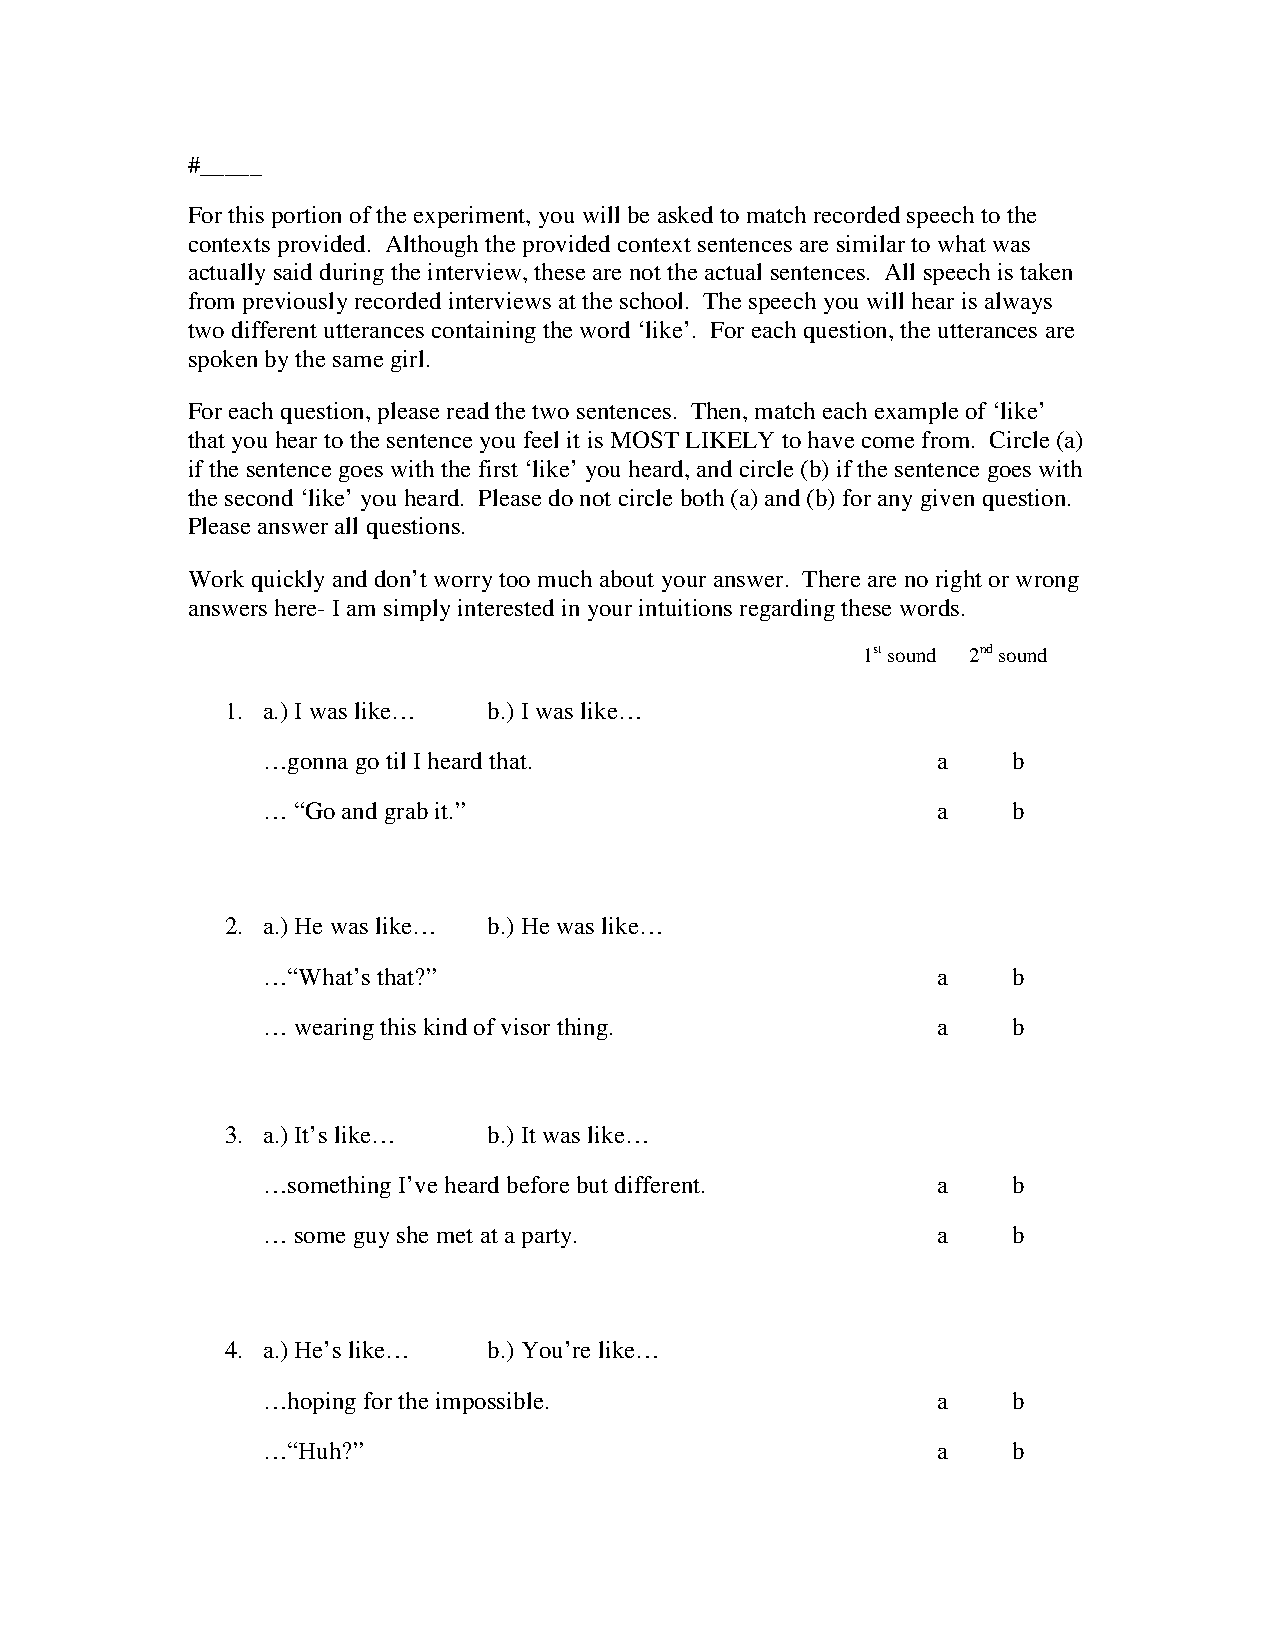
\includegraphics[width=5in]{images/Exp1page1.pdf}
		\caption{Answersheet for Experiment 1}
		\label{x1p1}
\end{figure}

\begin{figure}[htbp]
	\centering
		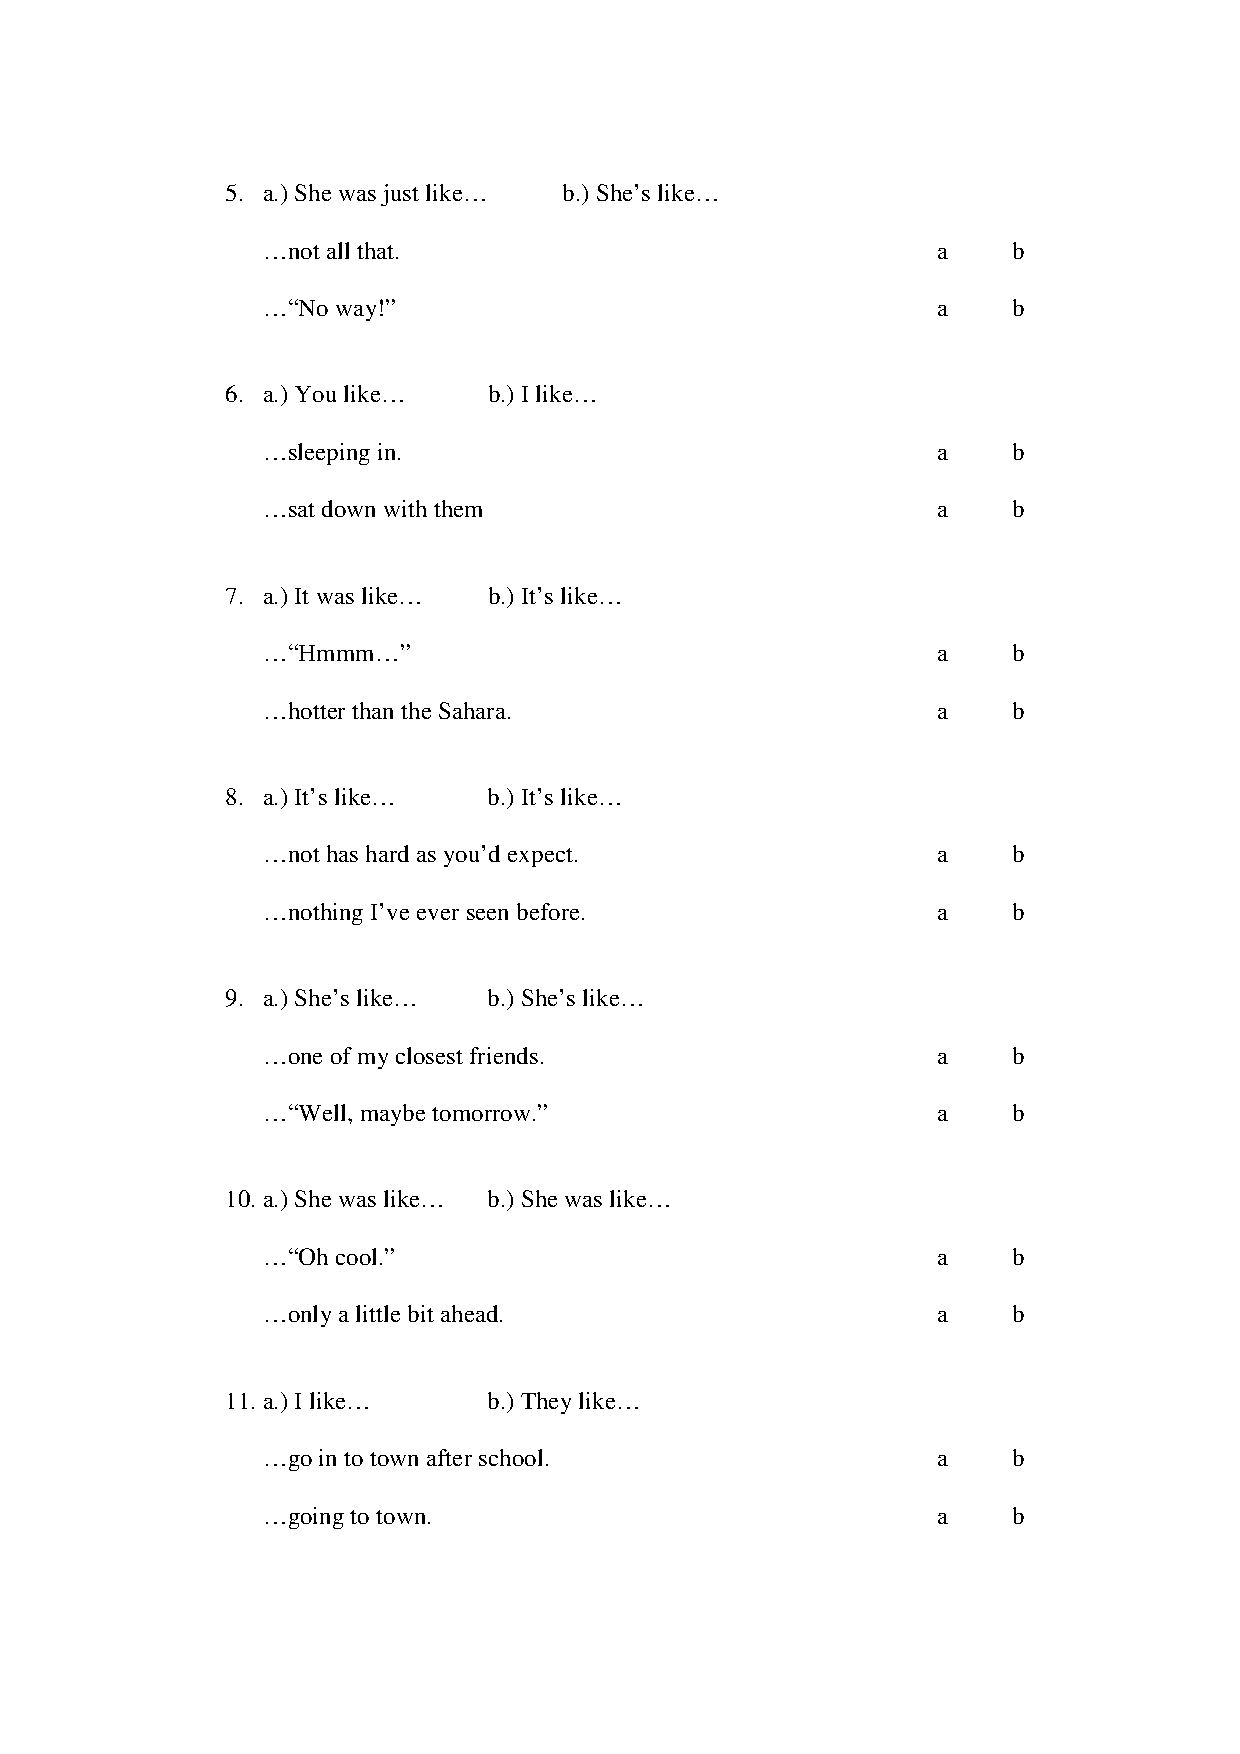
\includegraphics[width=5in]{images/Exp1page2.pdf}
		\label{x1p2}
\end{figure}

\begin{figure}[htbp]
	\centering
		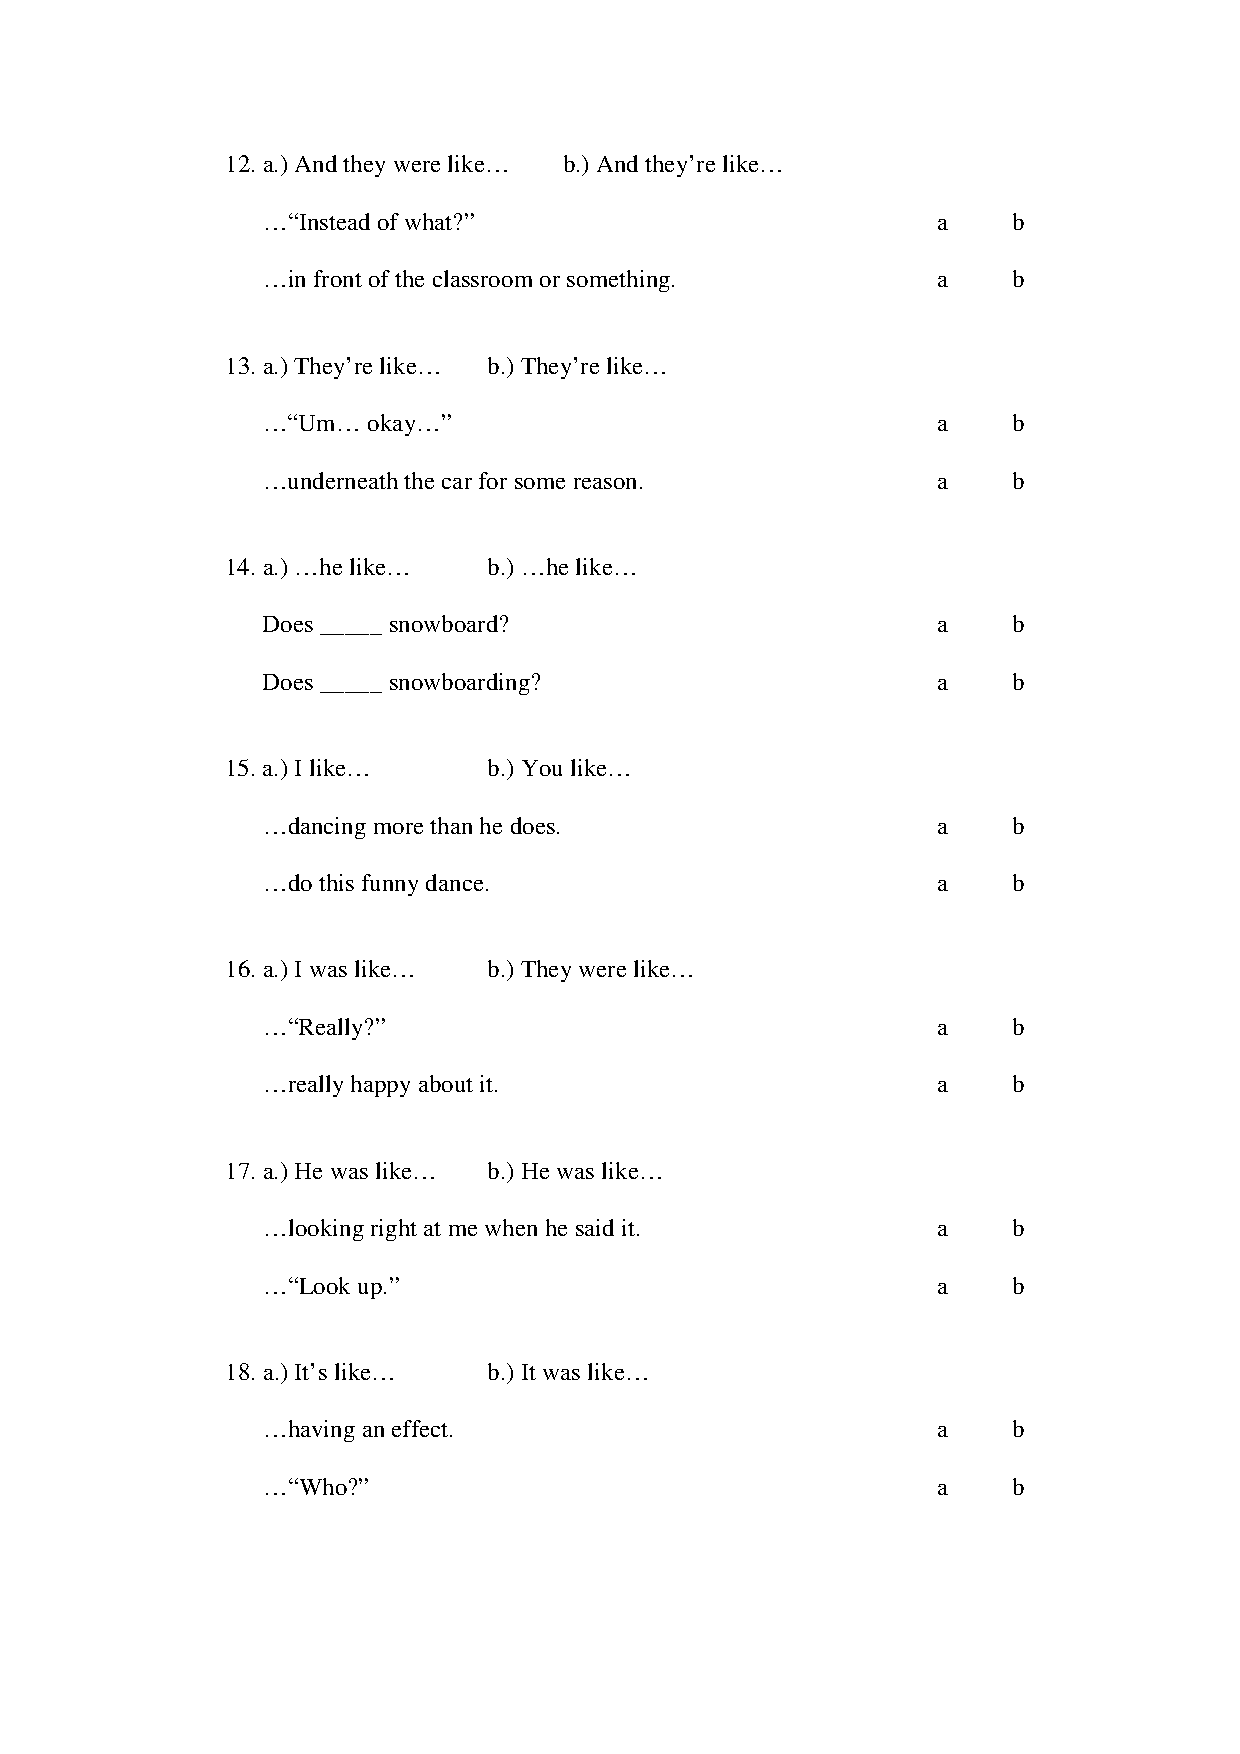
\includegraphics[width=5in]{images/Exp1page3.pdf}
		\label{x1p3}
\end{figure}

\begin{figure}[htbp]
	\centering
		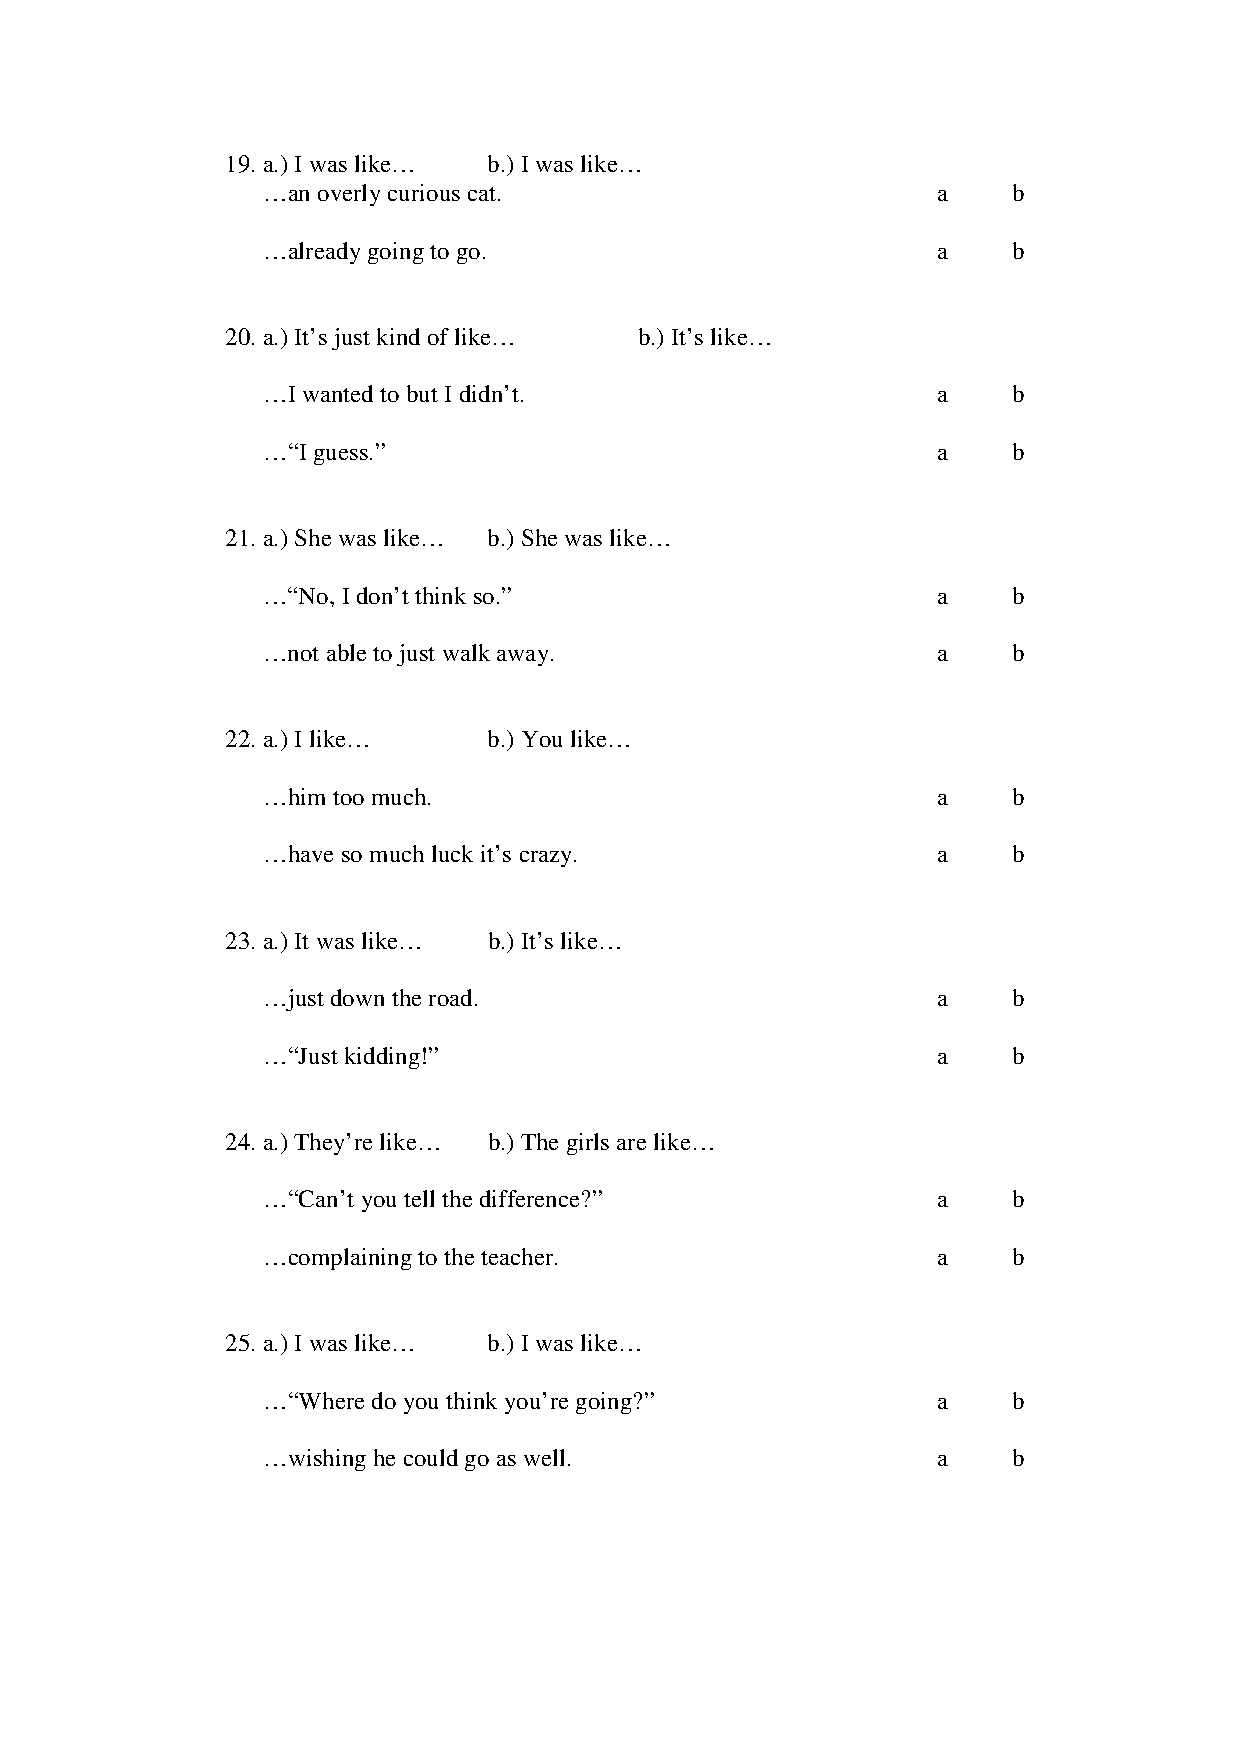
\includegraphics[width=5in]{images/Exp1page4.pdf}
		\label{x1p4}
\end{figure}

\begin{figure}[htbp]
	\centering
		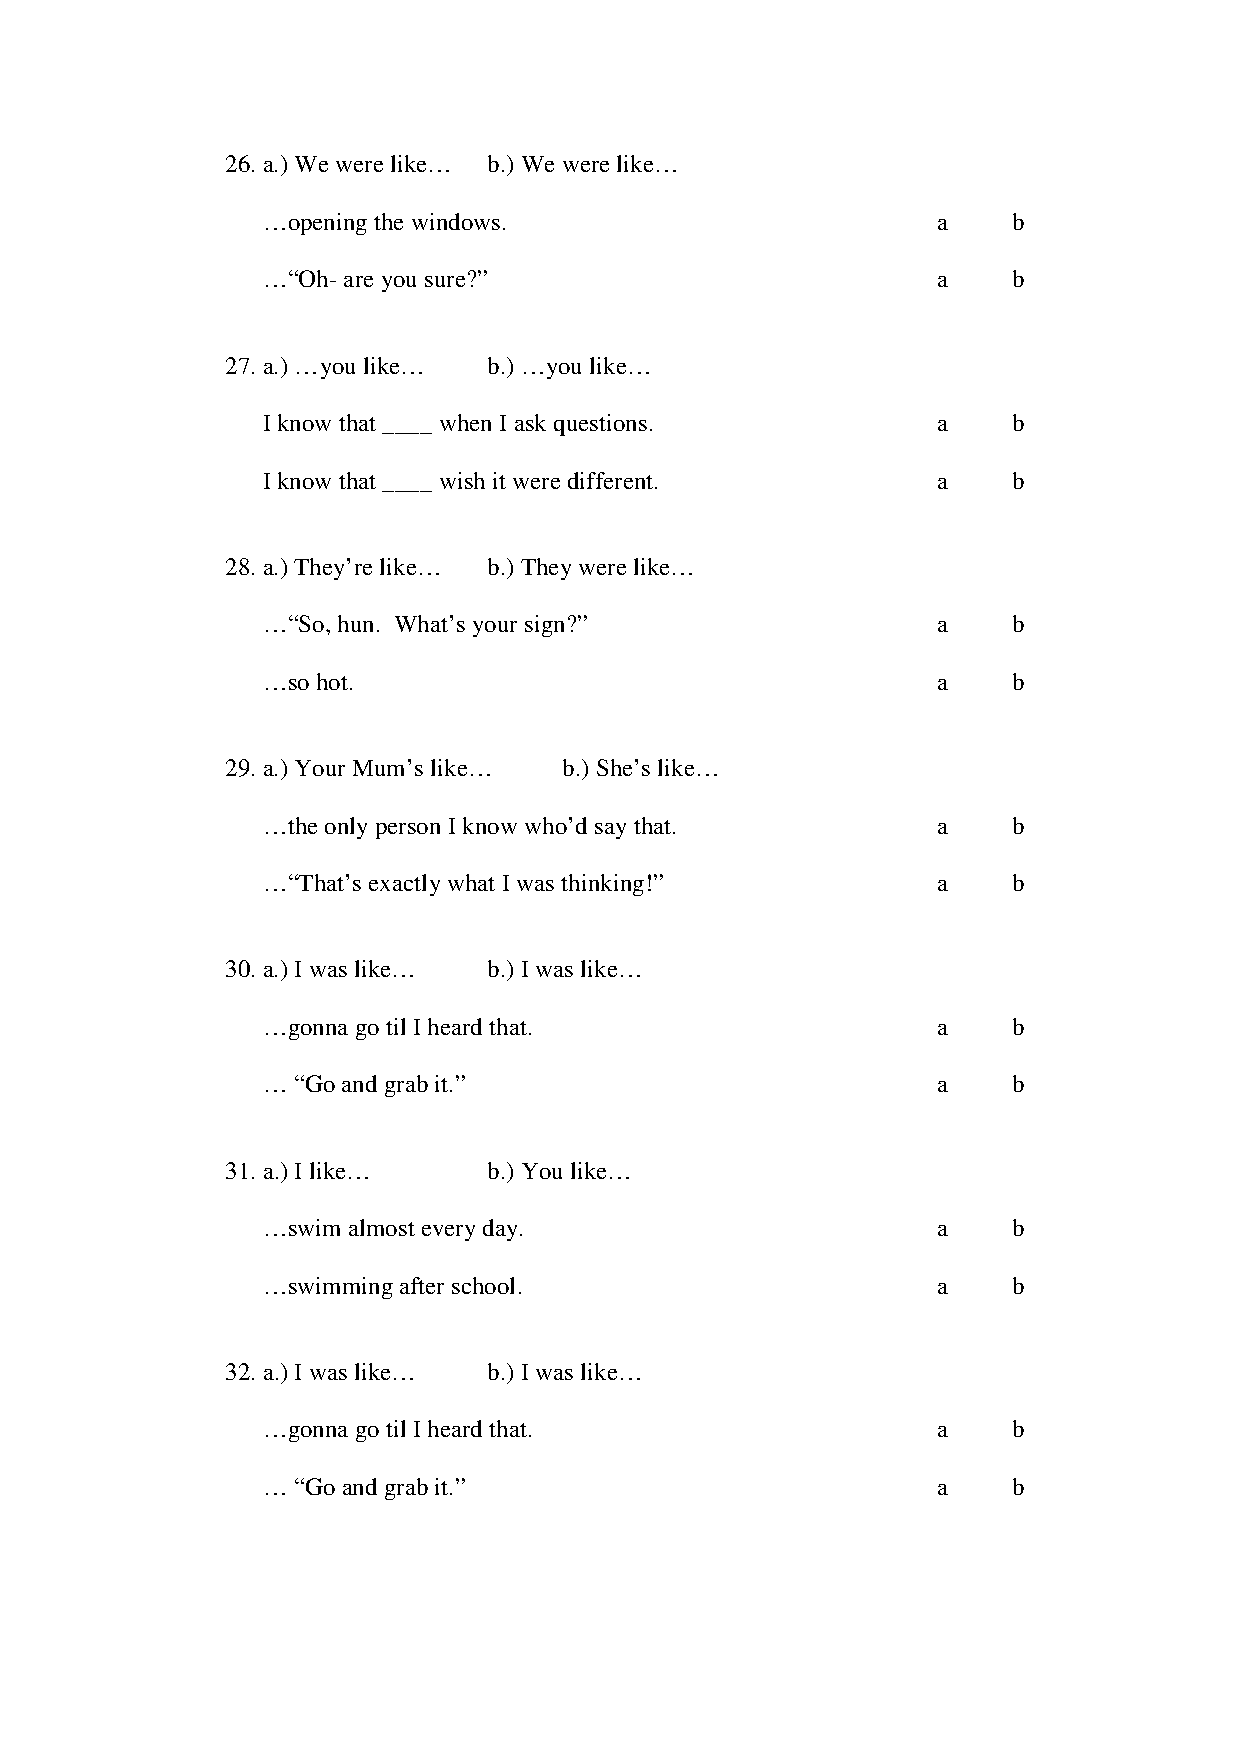
\includegraphics[width=5in]{images/Exp1page5.pdf}
		\label{x1p5}
\end{figure}

\begin{figure}[htbp]
	\centering
		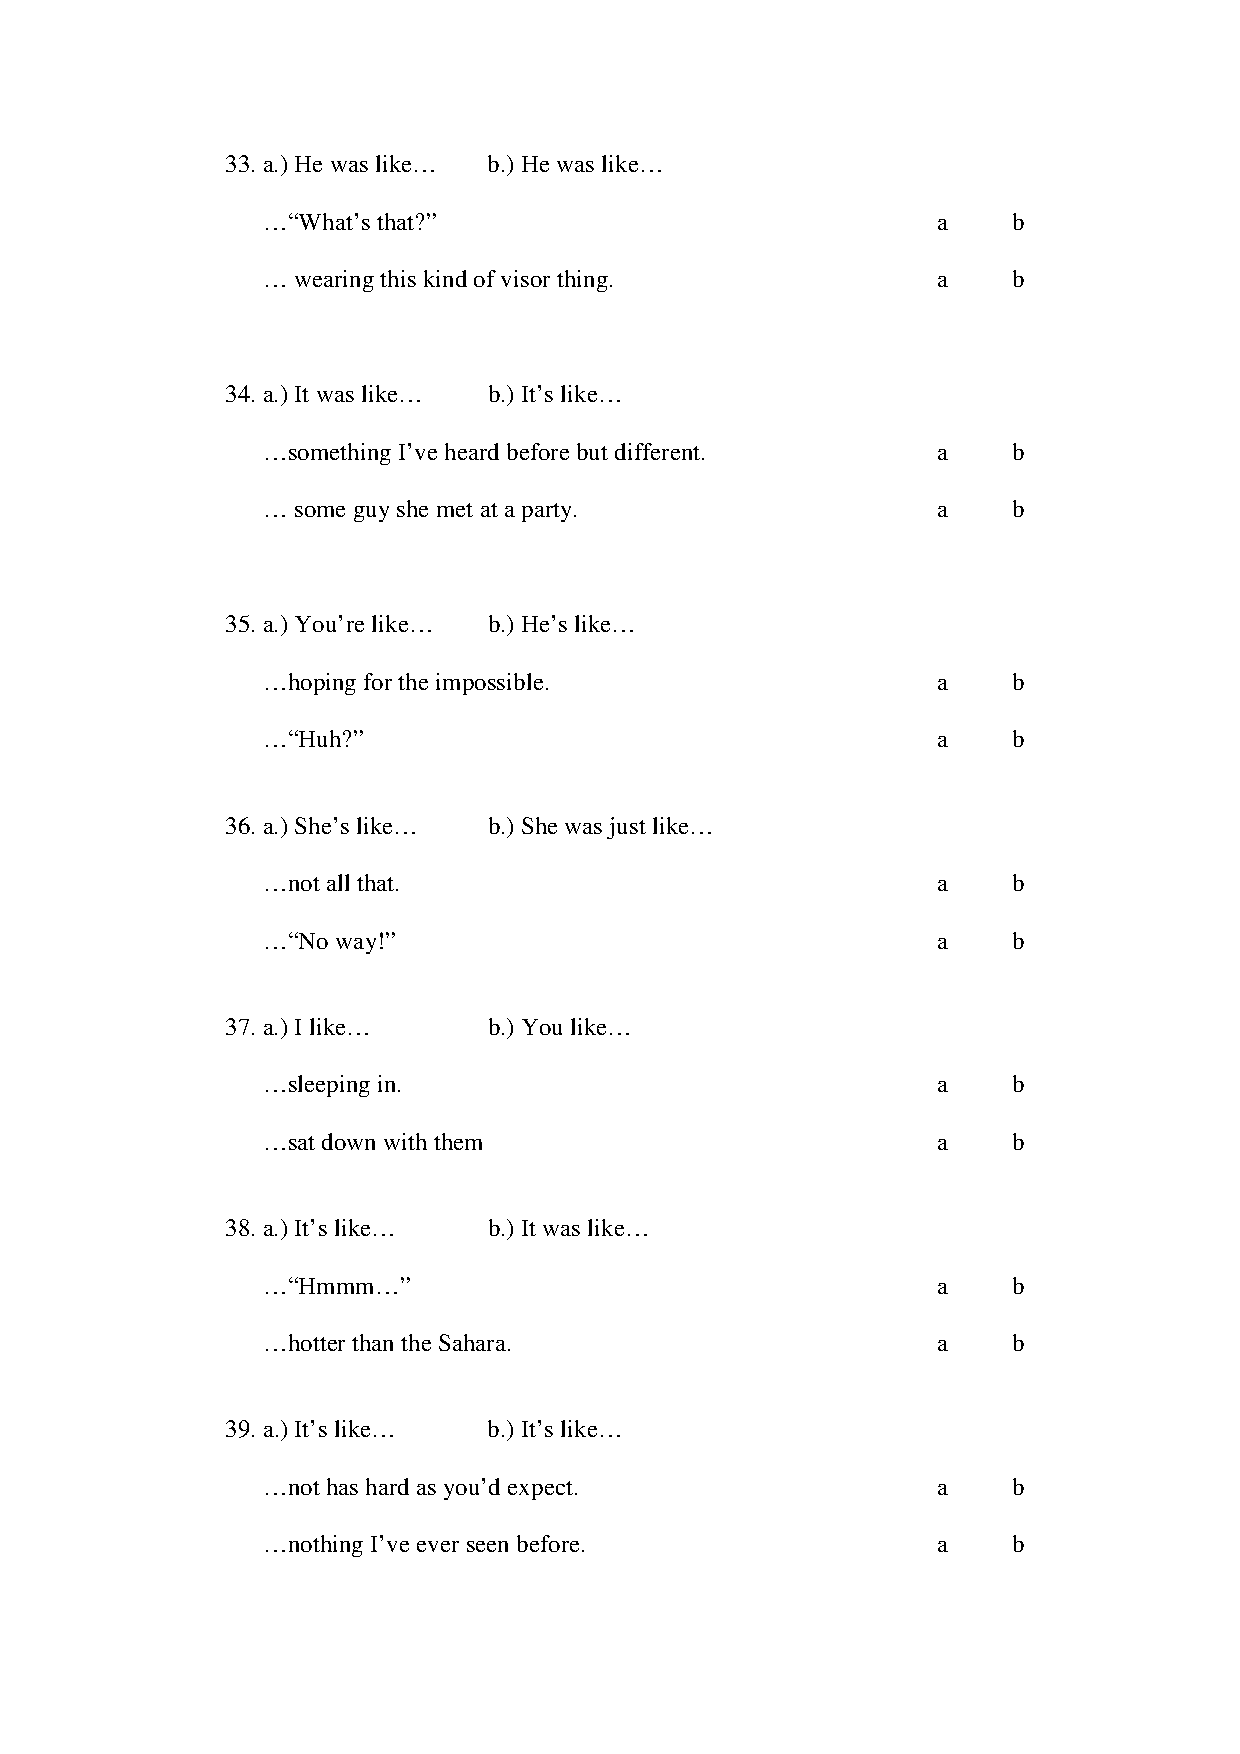
\includegraphics[width=5in]{images/Exp1page6.pdf}
	\label{x1p6}
\end{figure}

\begin{figure}[htbp]
	\centering
		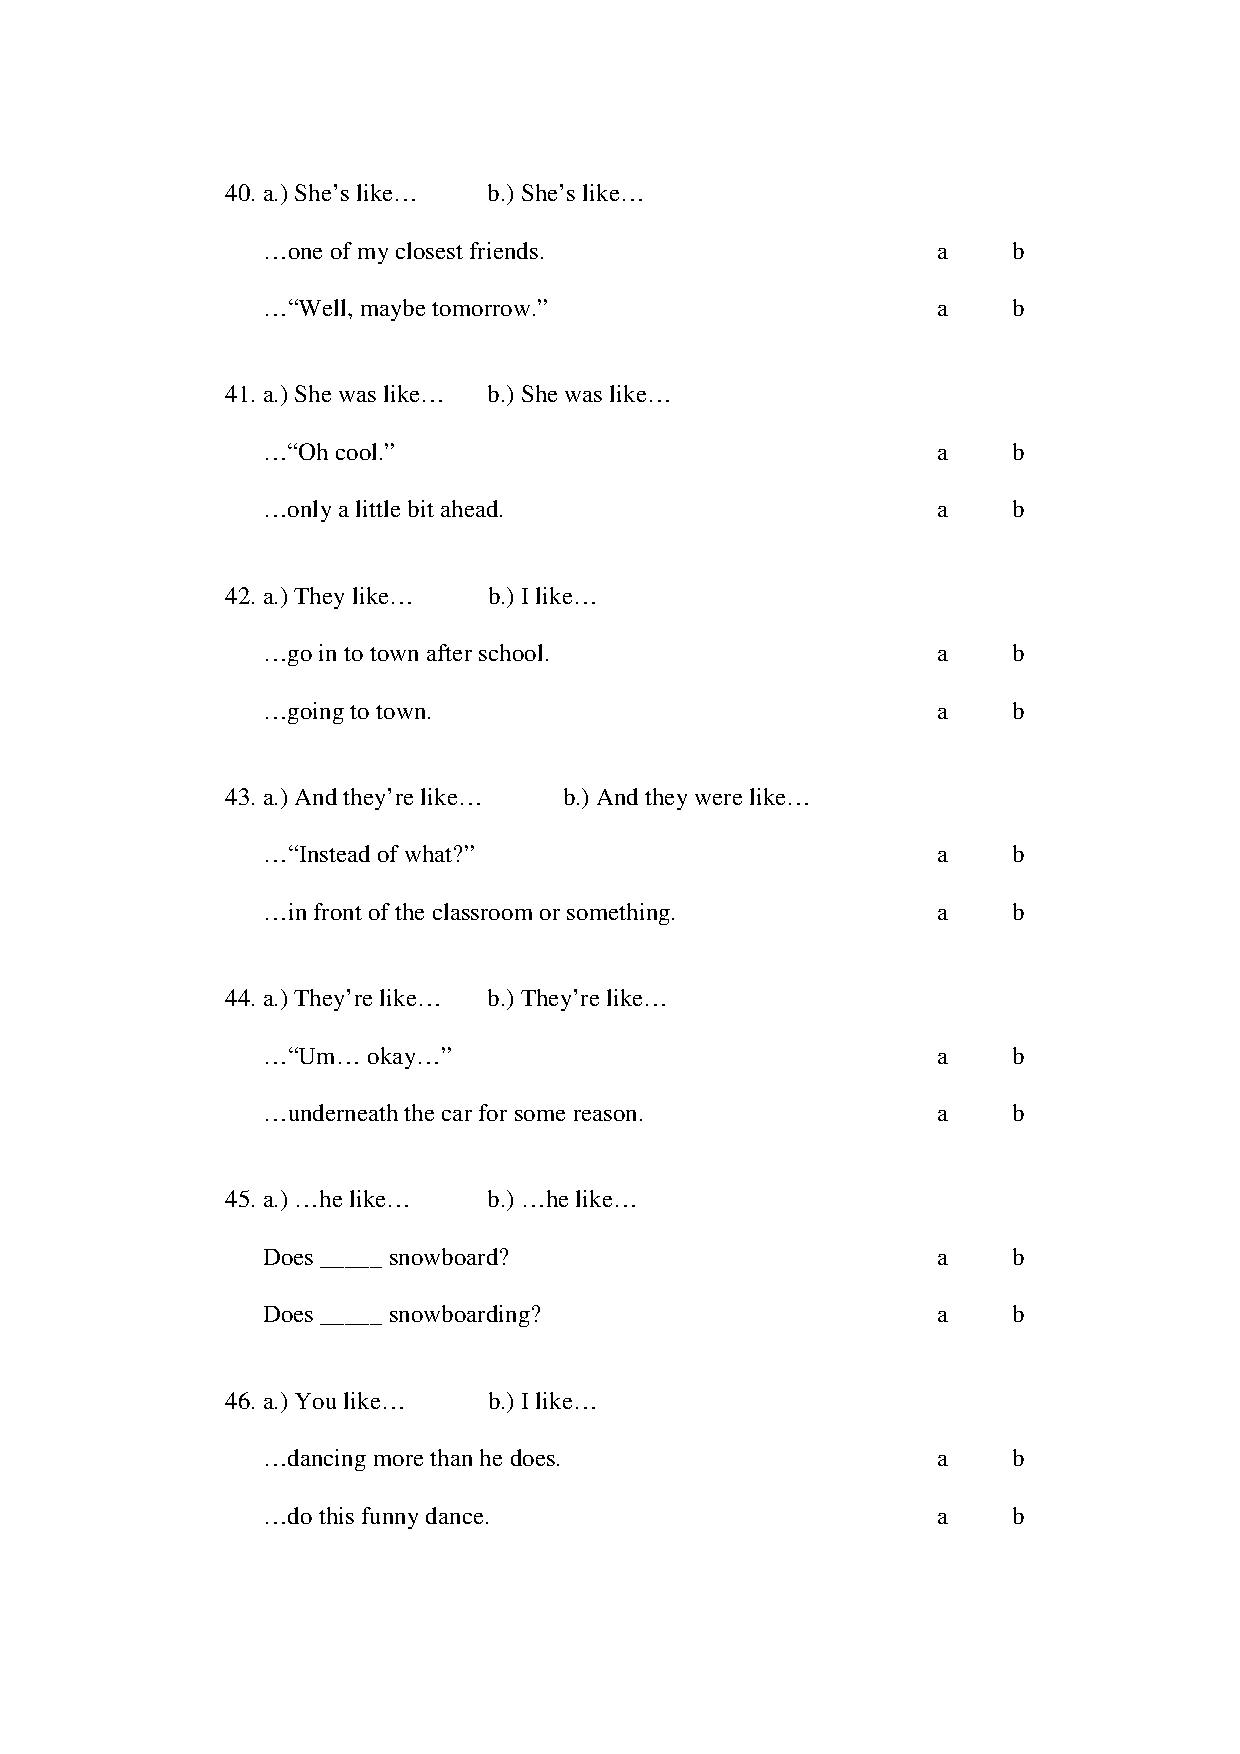
\includegraphics[width=5in]{images/Exp1page7.pdf}
	\label{x1p7}
\end{figure}

\begin{figure}[htbp]
	\centering
		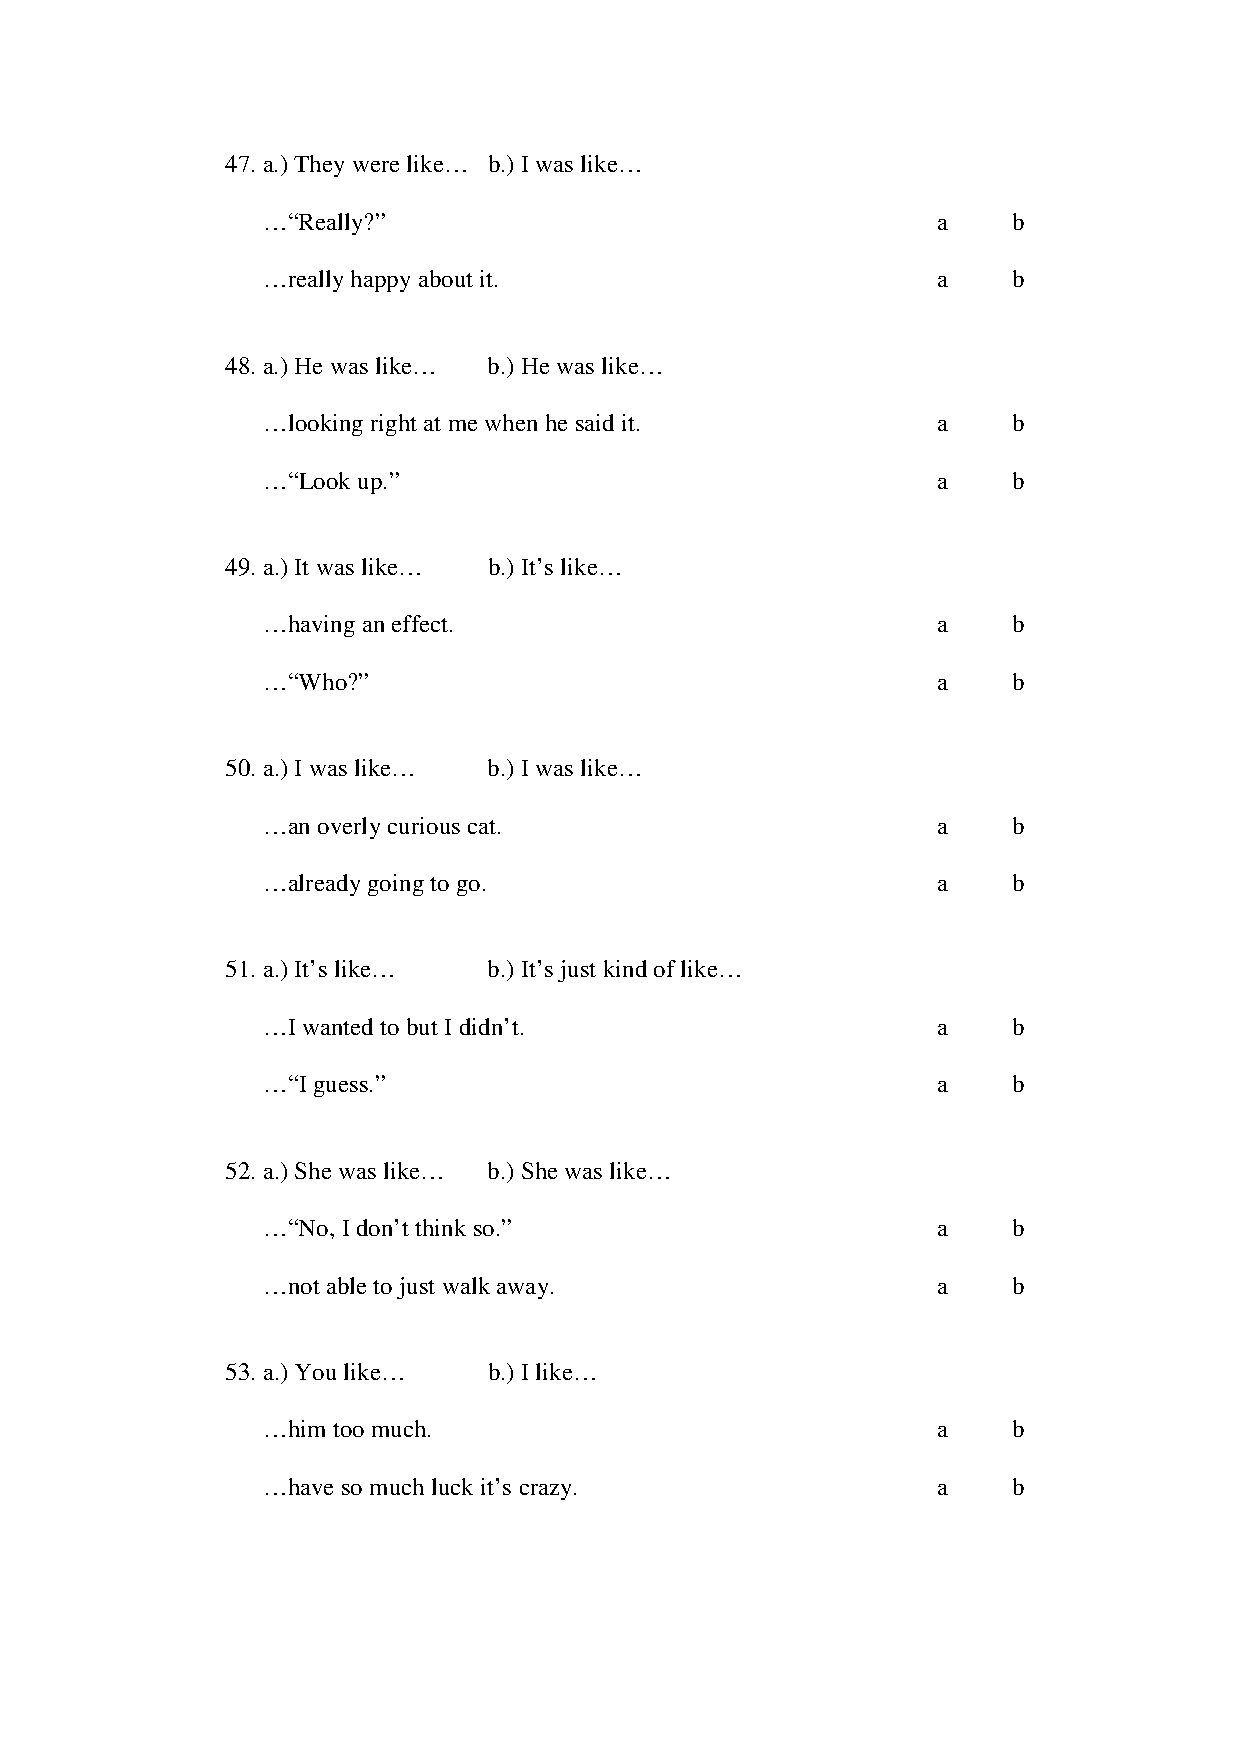
\includegraphics[width=5in]{images/Exp1page8.pdf}
		\label{x1p8}
\end{figure}

\begin{figure}[htbp]
	\centering
		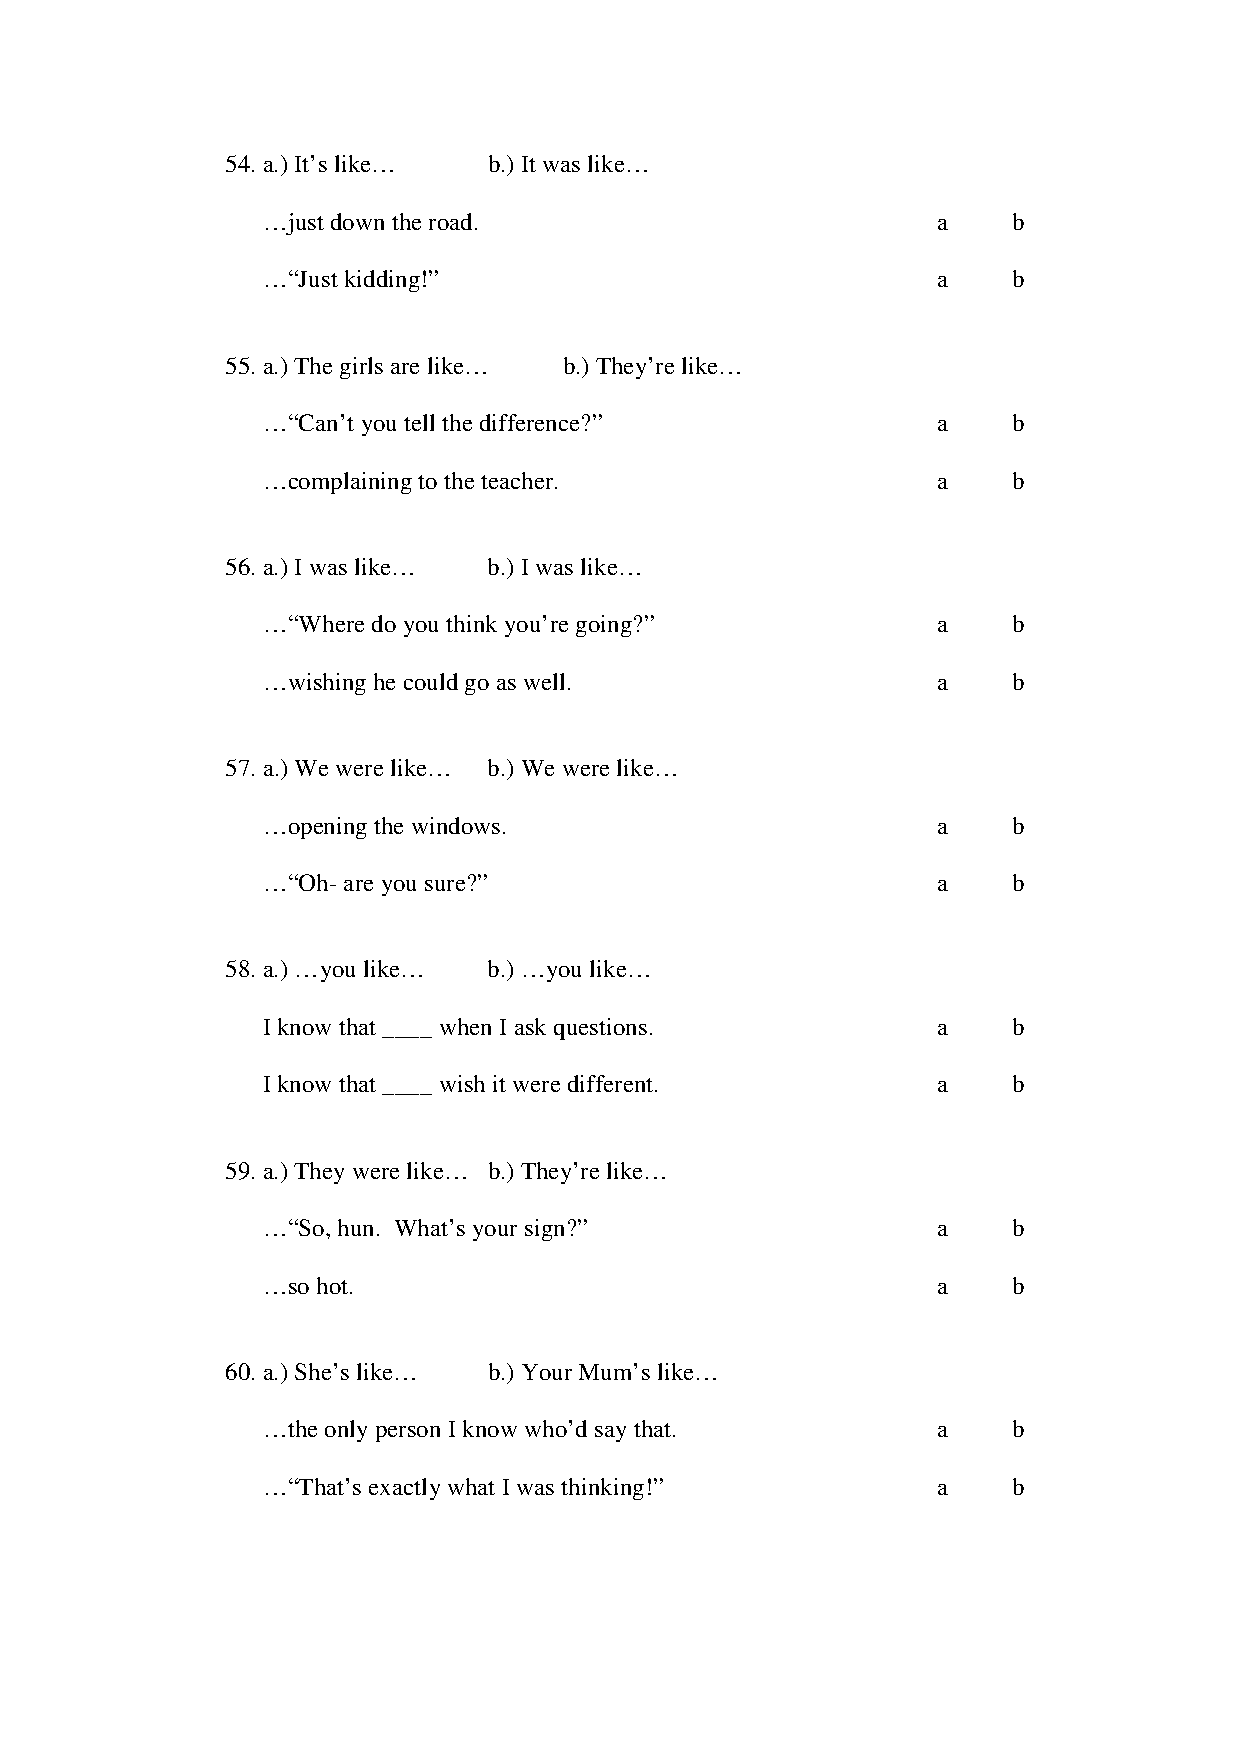
\includegraphics[width=5in]{images/Exp1page9.pdf}
		\label{x1p9}
\end{figure}

\begin{figure}[htbp]
	\centering
		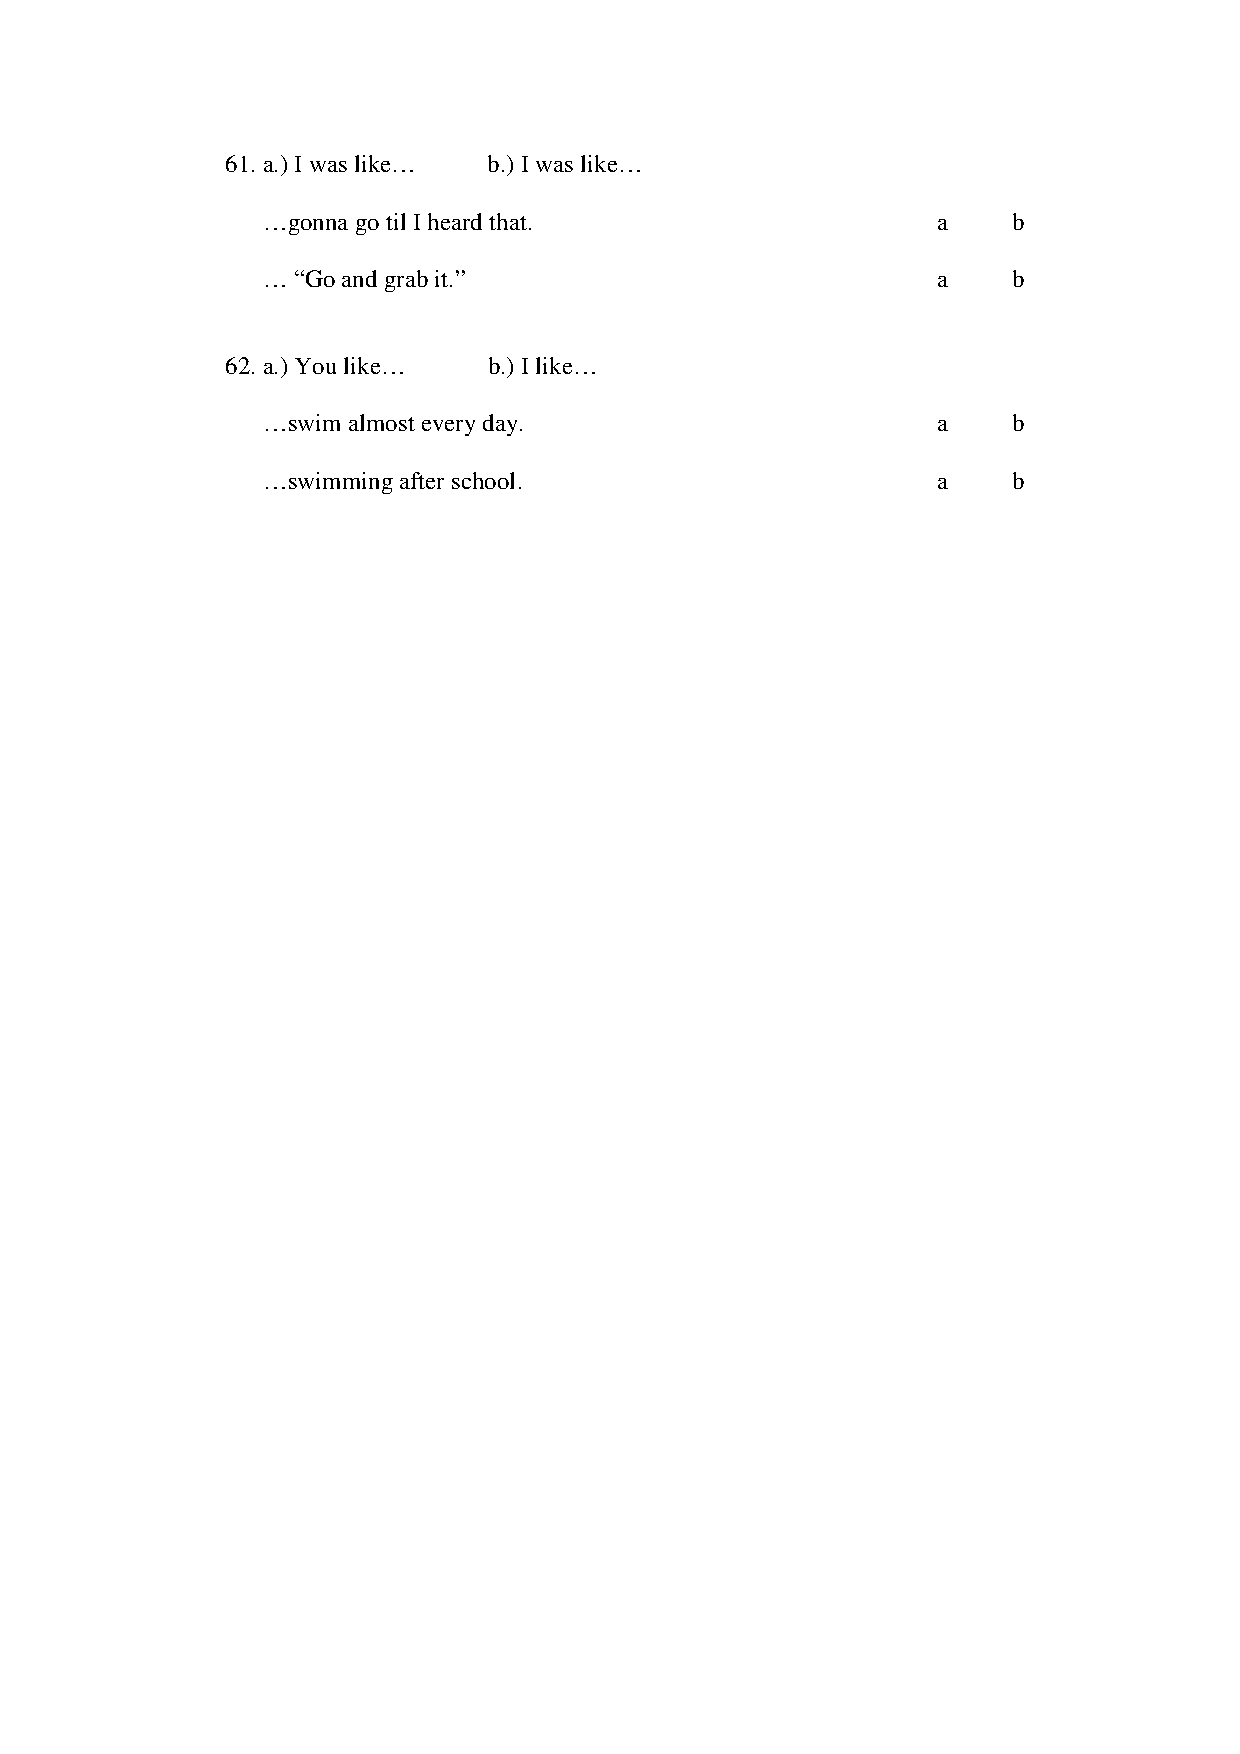
\includegraphics[width=5in]{images/Exp1page10.pdf}
		\label{x1p10}
\end{figure}


\clearpage
\begin{figure}[htbp]
	\centering
		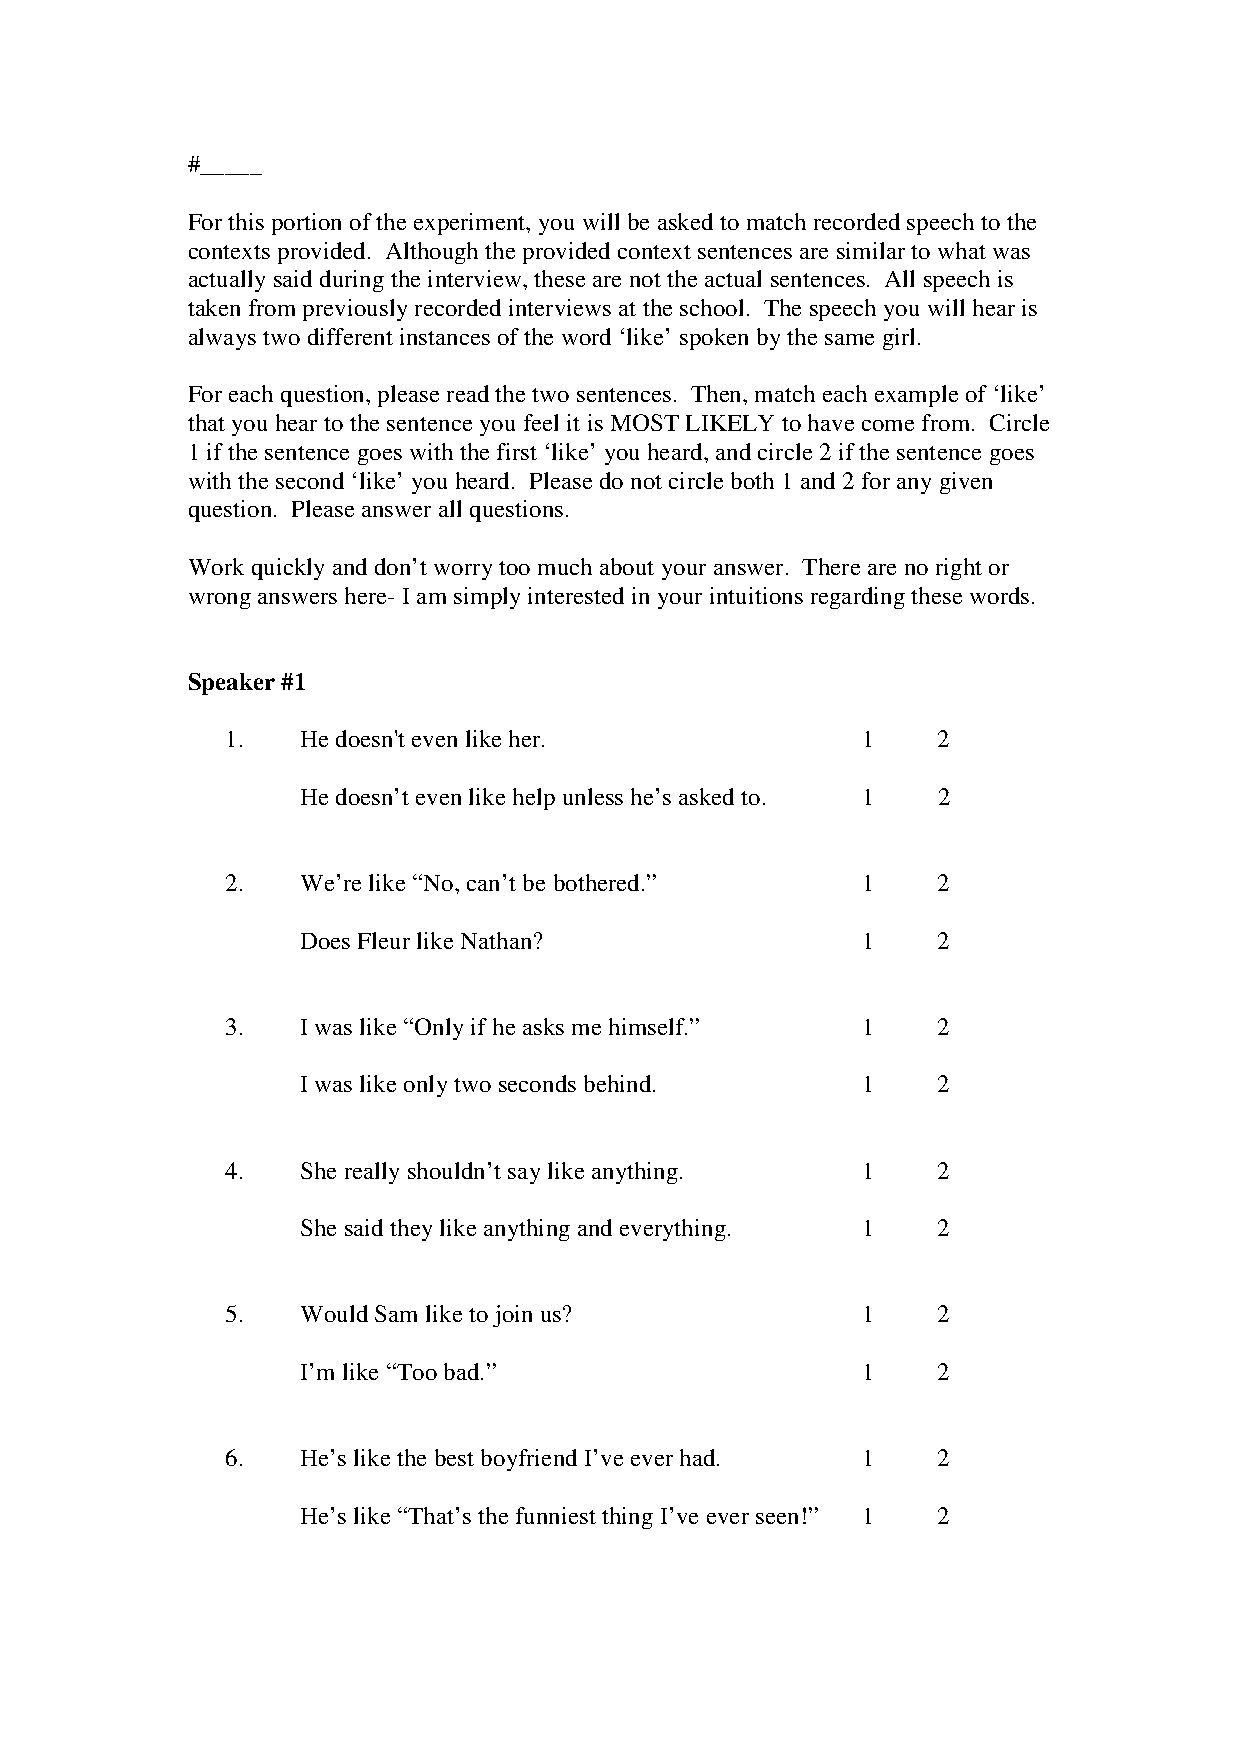
\includegraphics[width=5in]{images/Exp2page1.pdf}
		\caption{Answersheet for Experiment 2}
		\label{x2p1}
\end{figure}

\begin{figure}
	\centering
		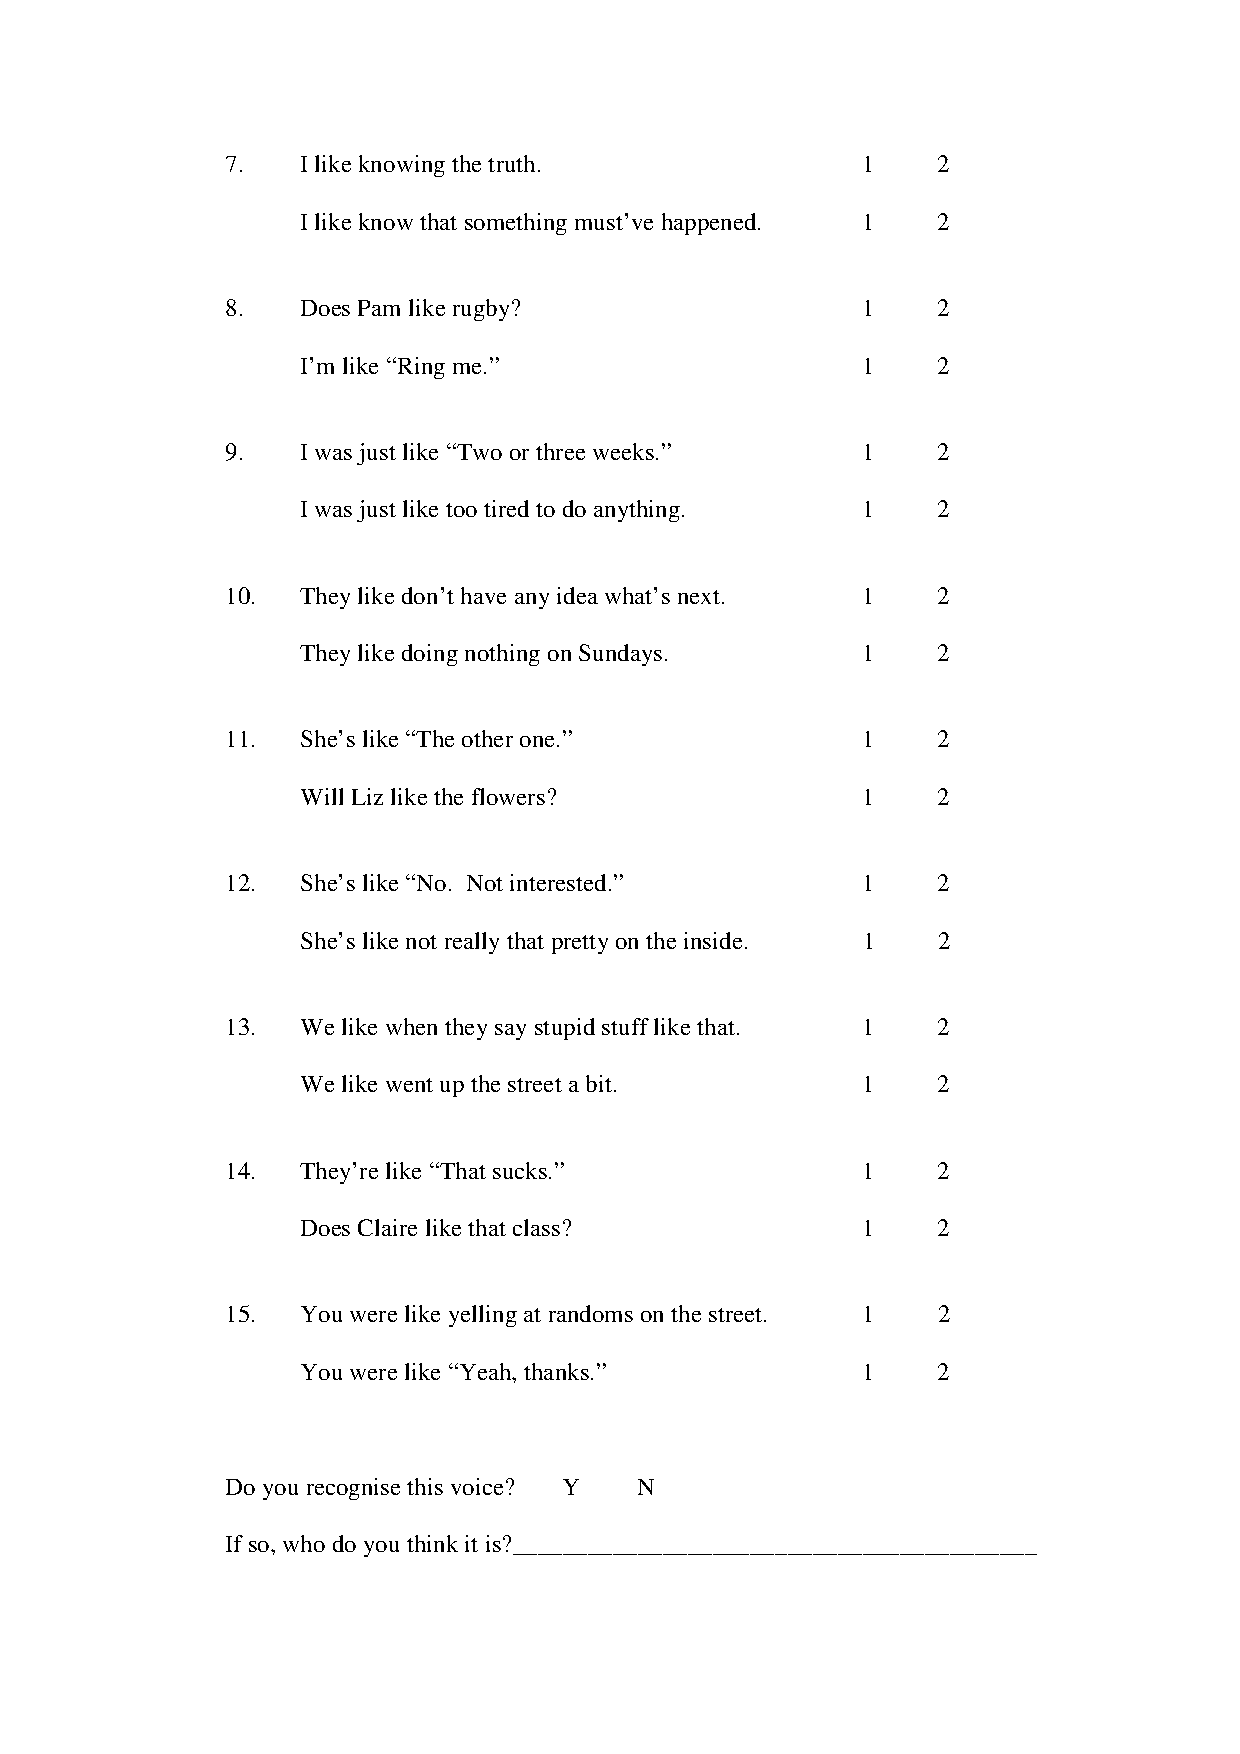
\includegraphics[width=5in]{images/Exp2page2.pdf}
			\label{x2p2}
\end{figure}

\begin{figure}
	\centering
		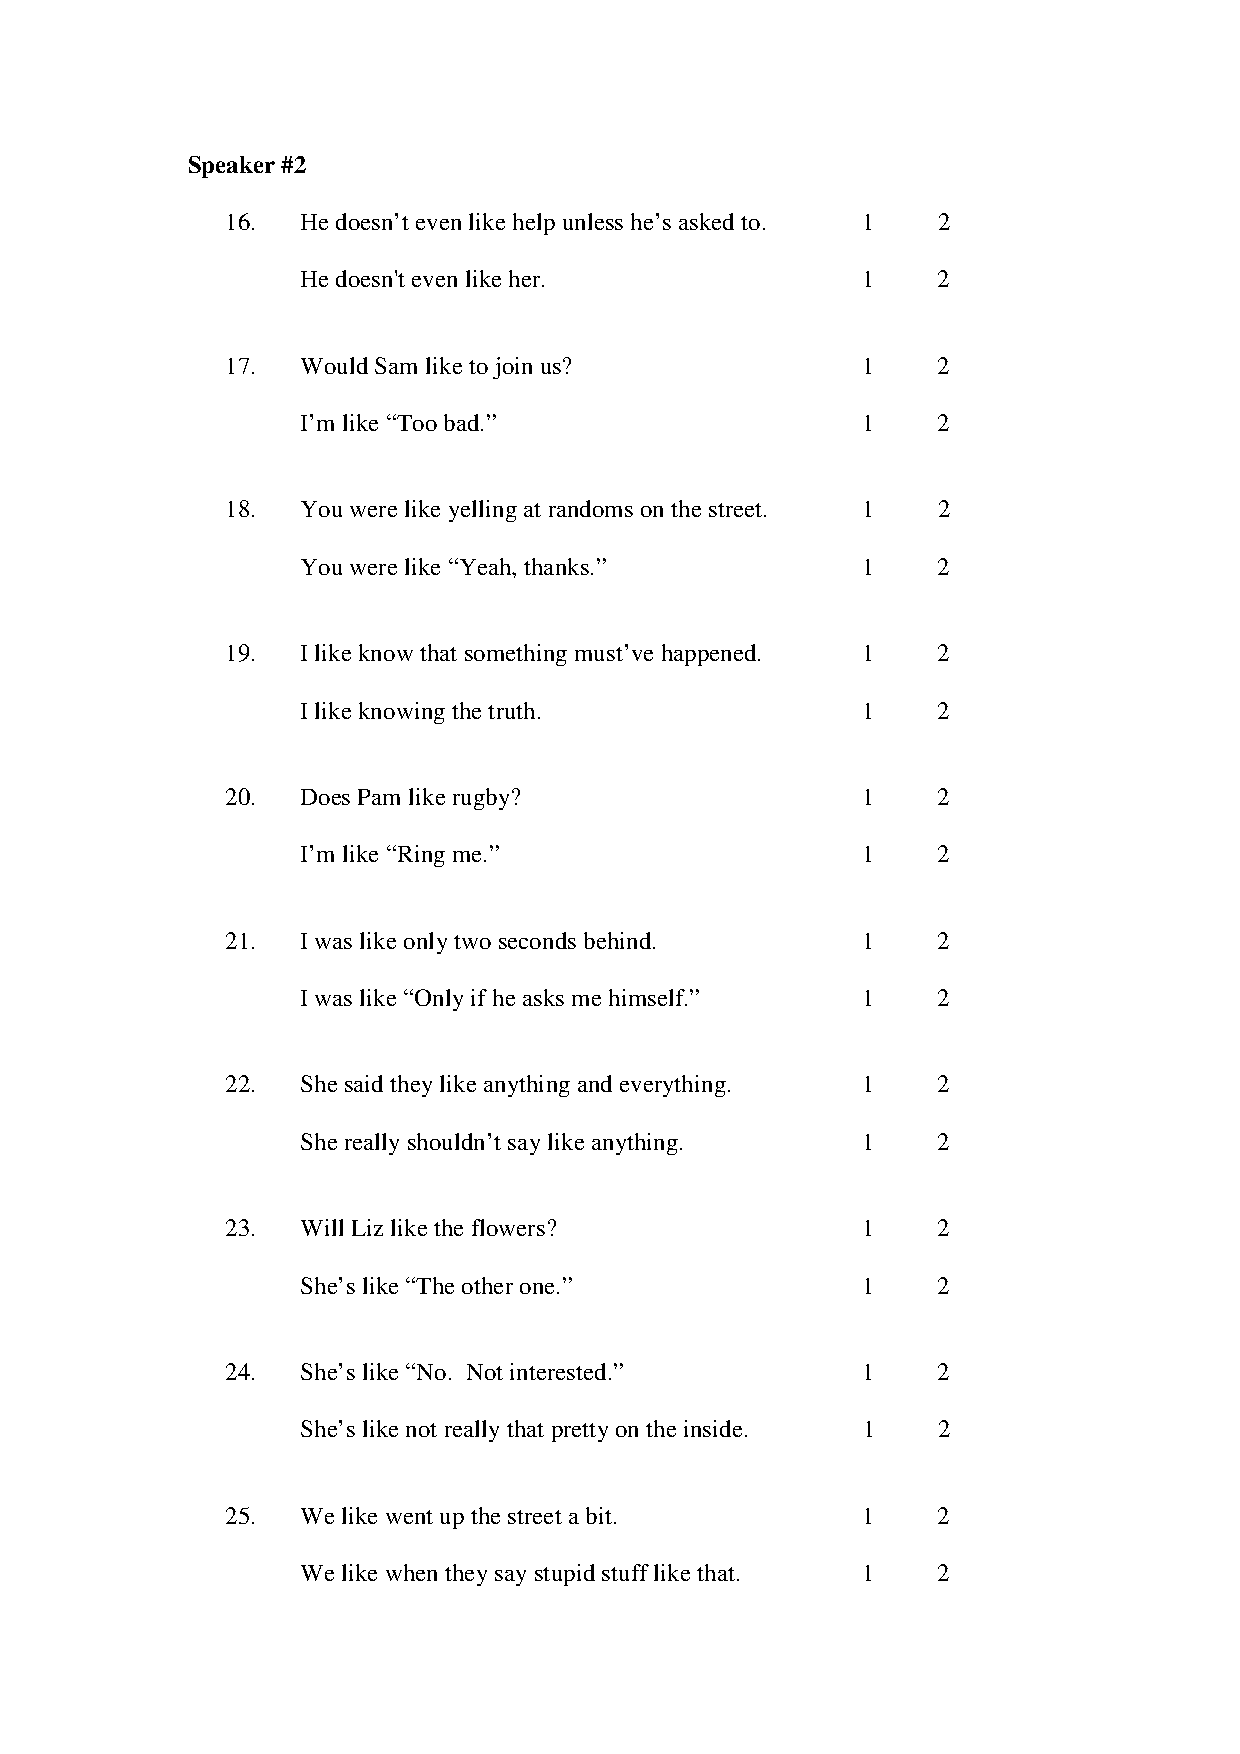
\includegraphics[width=5in]{images/Exp2page3.pdf}
			\label{x2p3}
\end{figure}

\begin{figure}
	\centering
		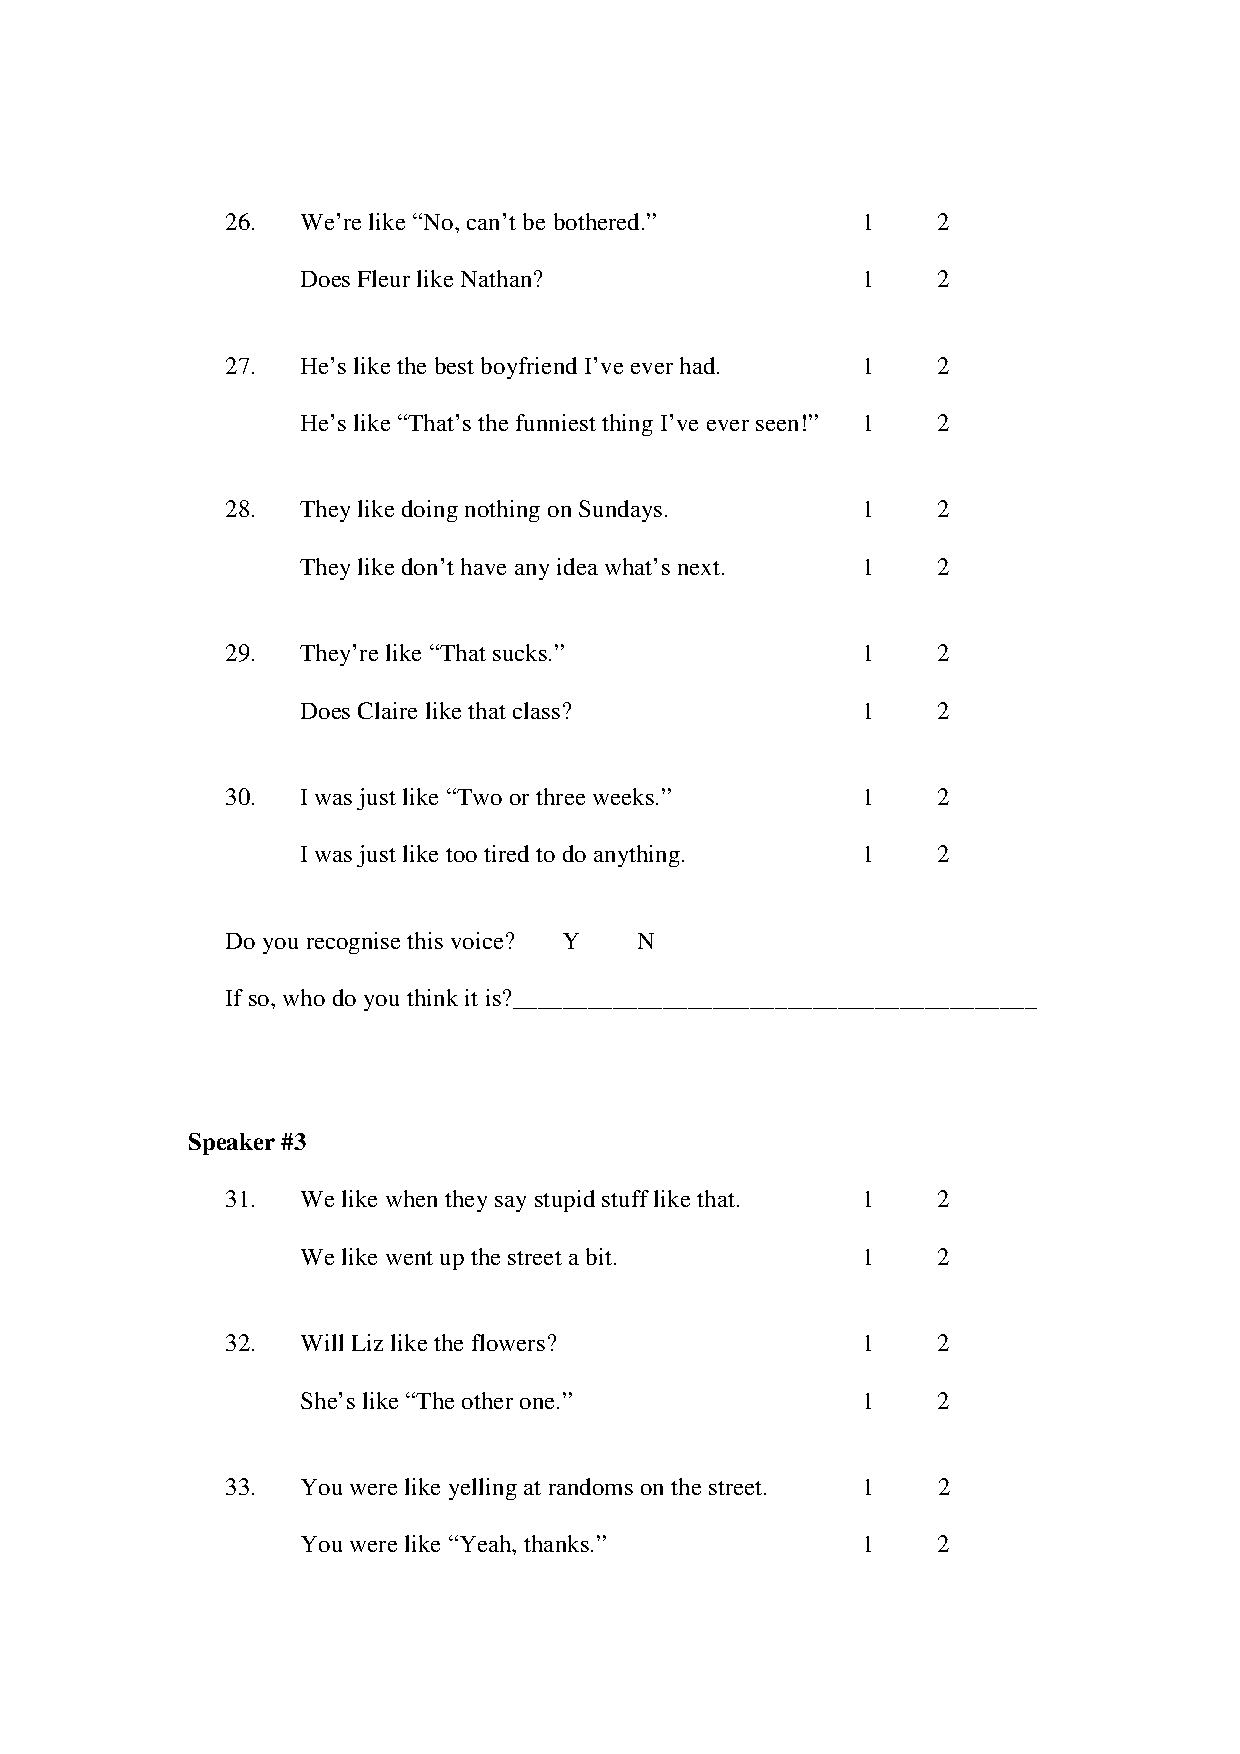
\includegraphics[width=5in]{images/Exp2page4.pdf}
			\label{x2p4}
\end{figure}

\begin{figure}
	\centering
		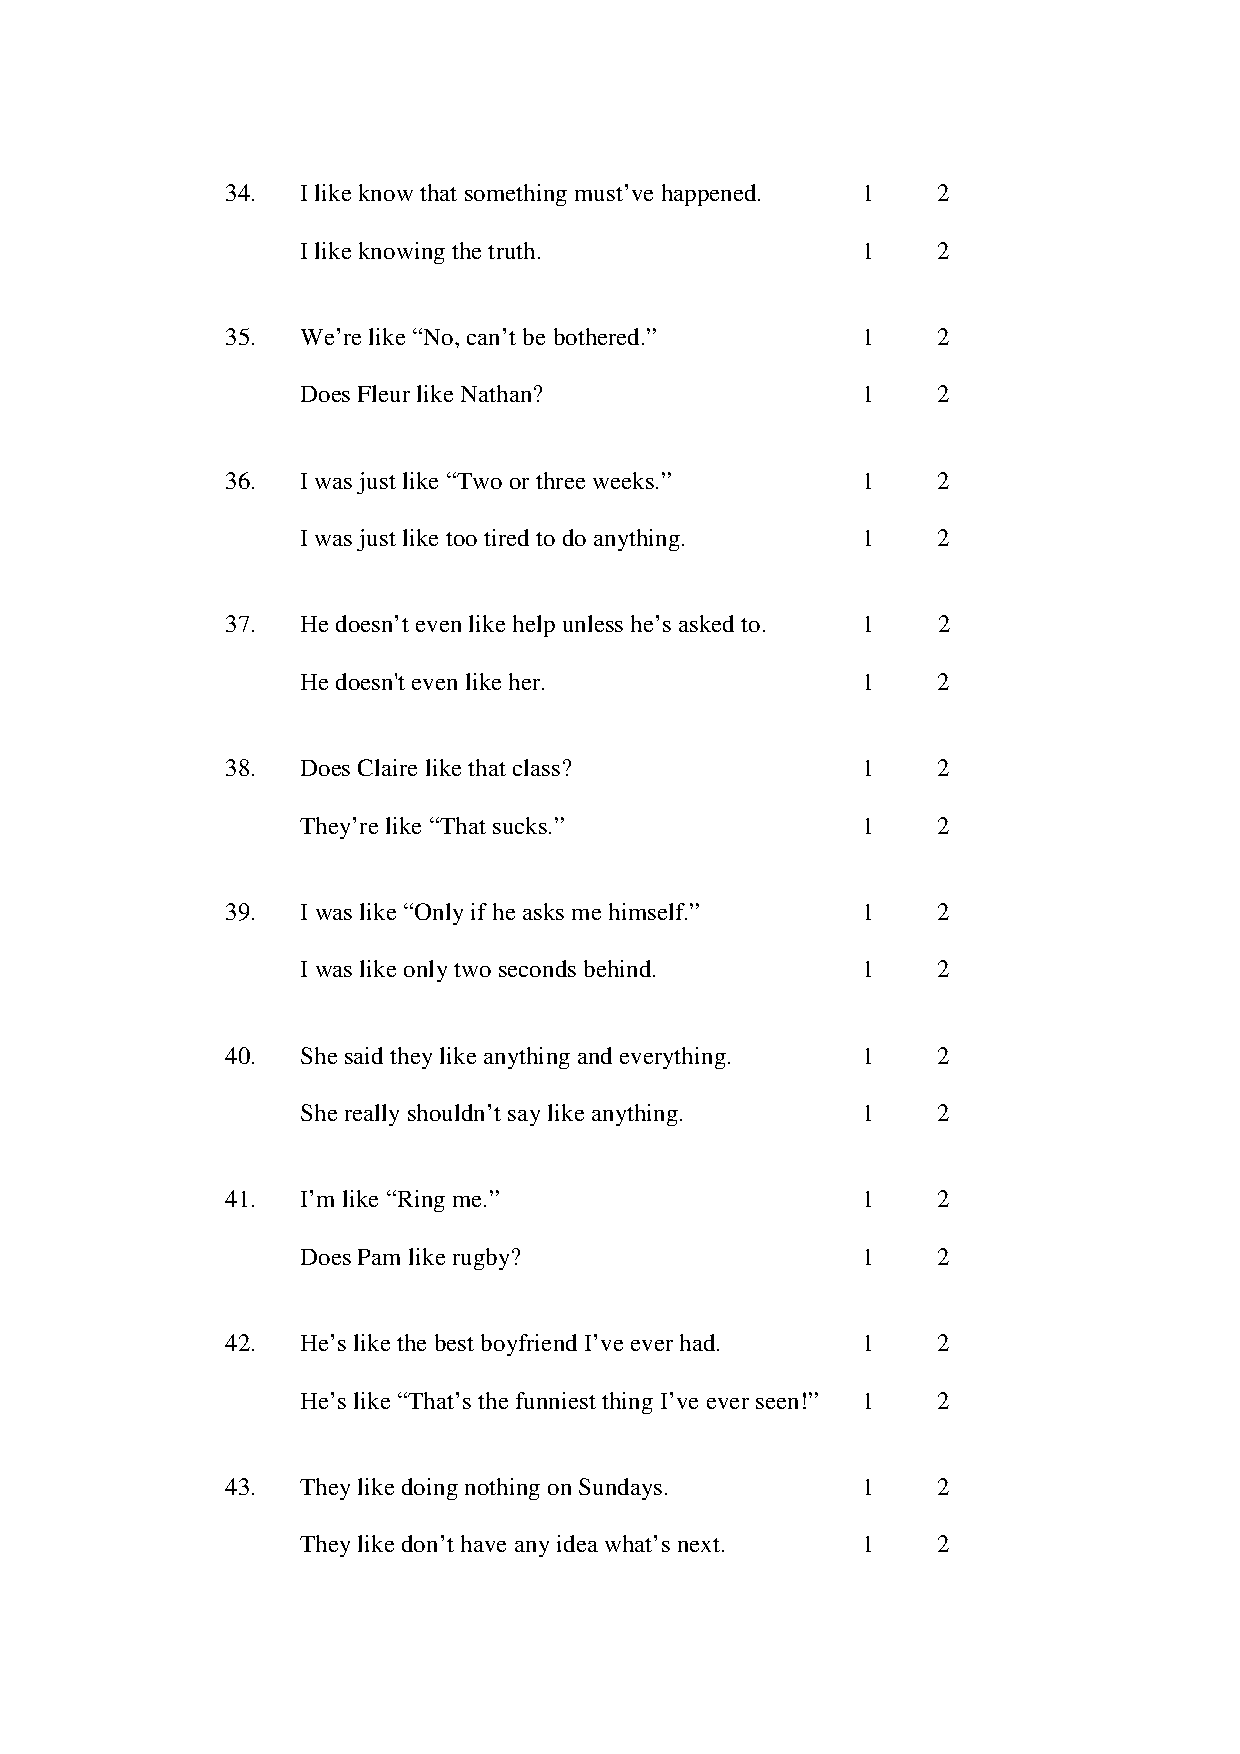
\includegraphics[width=5in]{images/Exp2page5.pdf}
			\label{x2p5}
\end{figure}

\begin{figure}
	\centering
		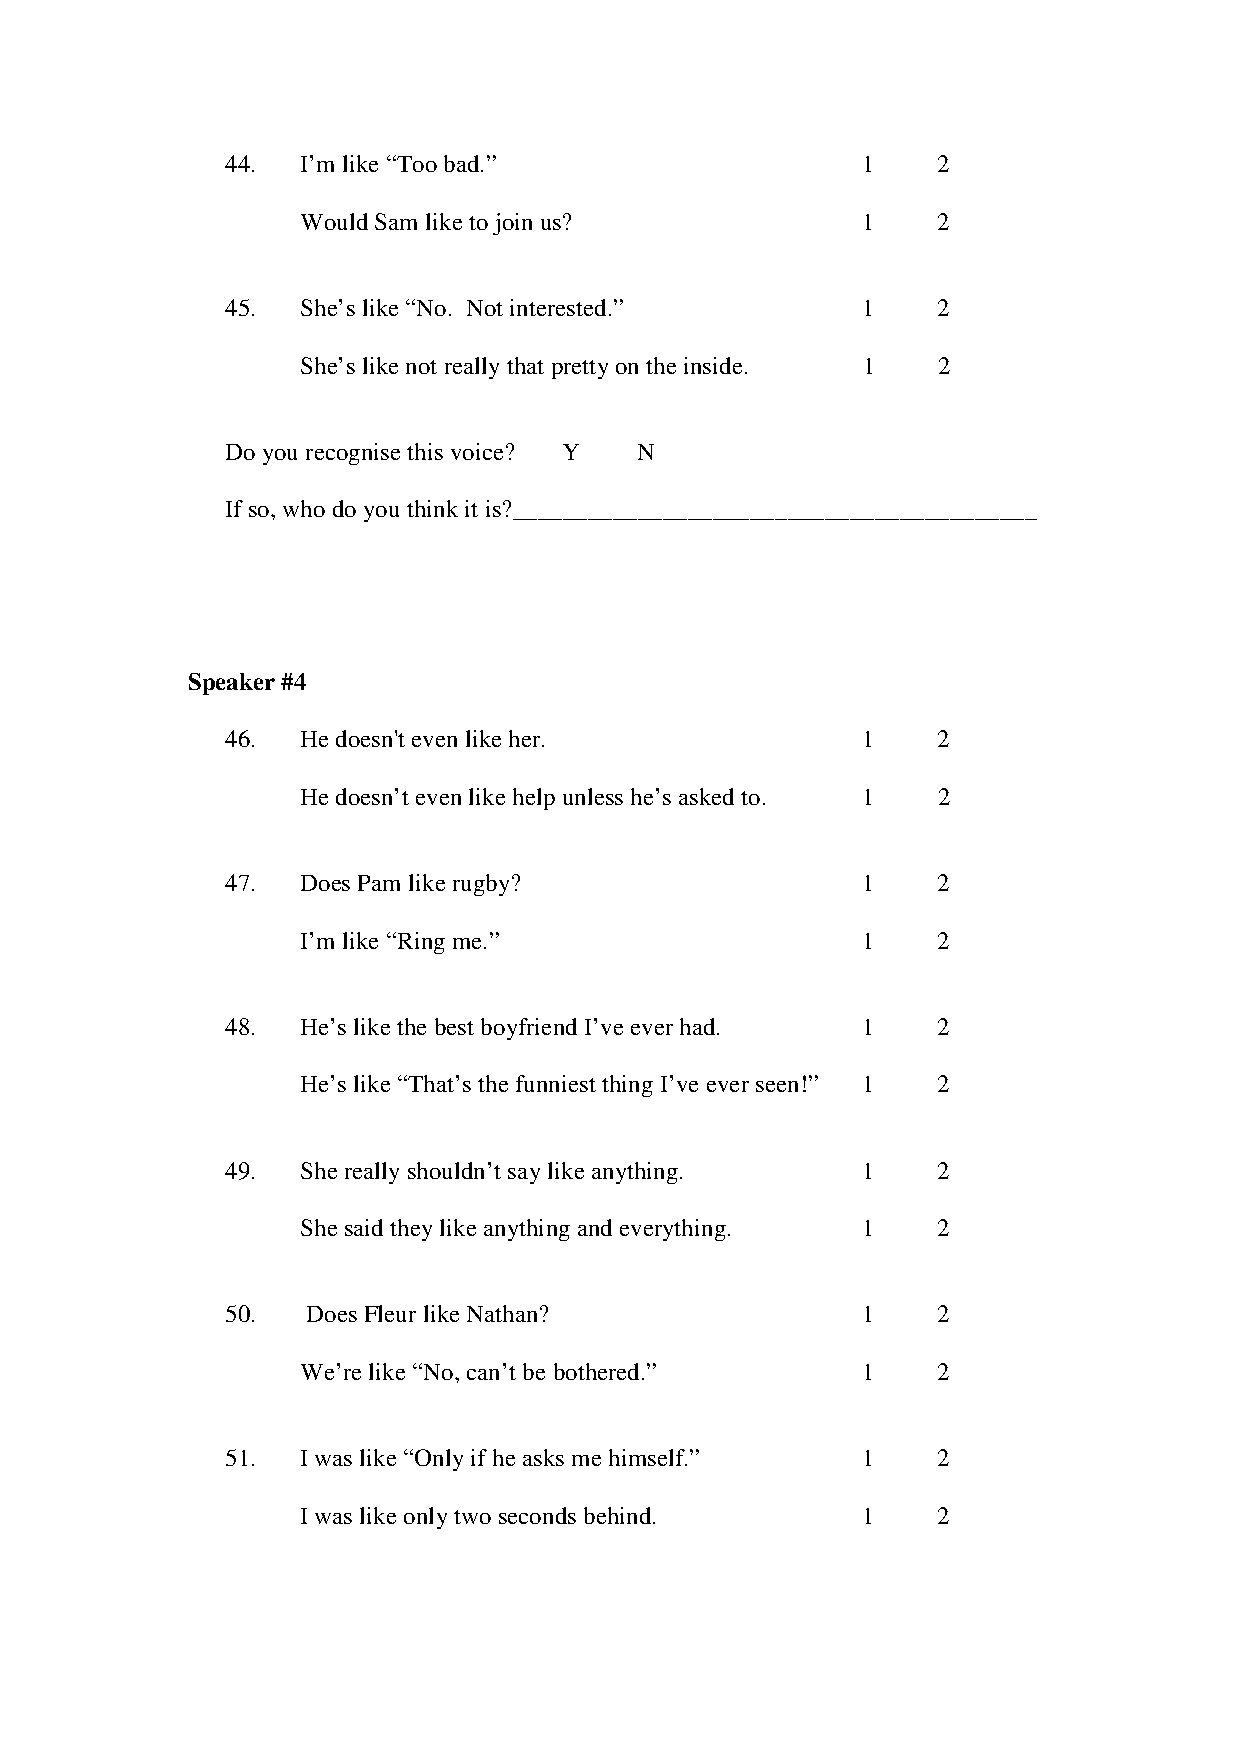
\includegraphics[width=5in]{images/Exp2page6.pdf}
			\label{x2p6}
\end{figure}

\begin{figure}
	\centering
		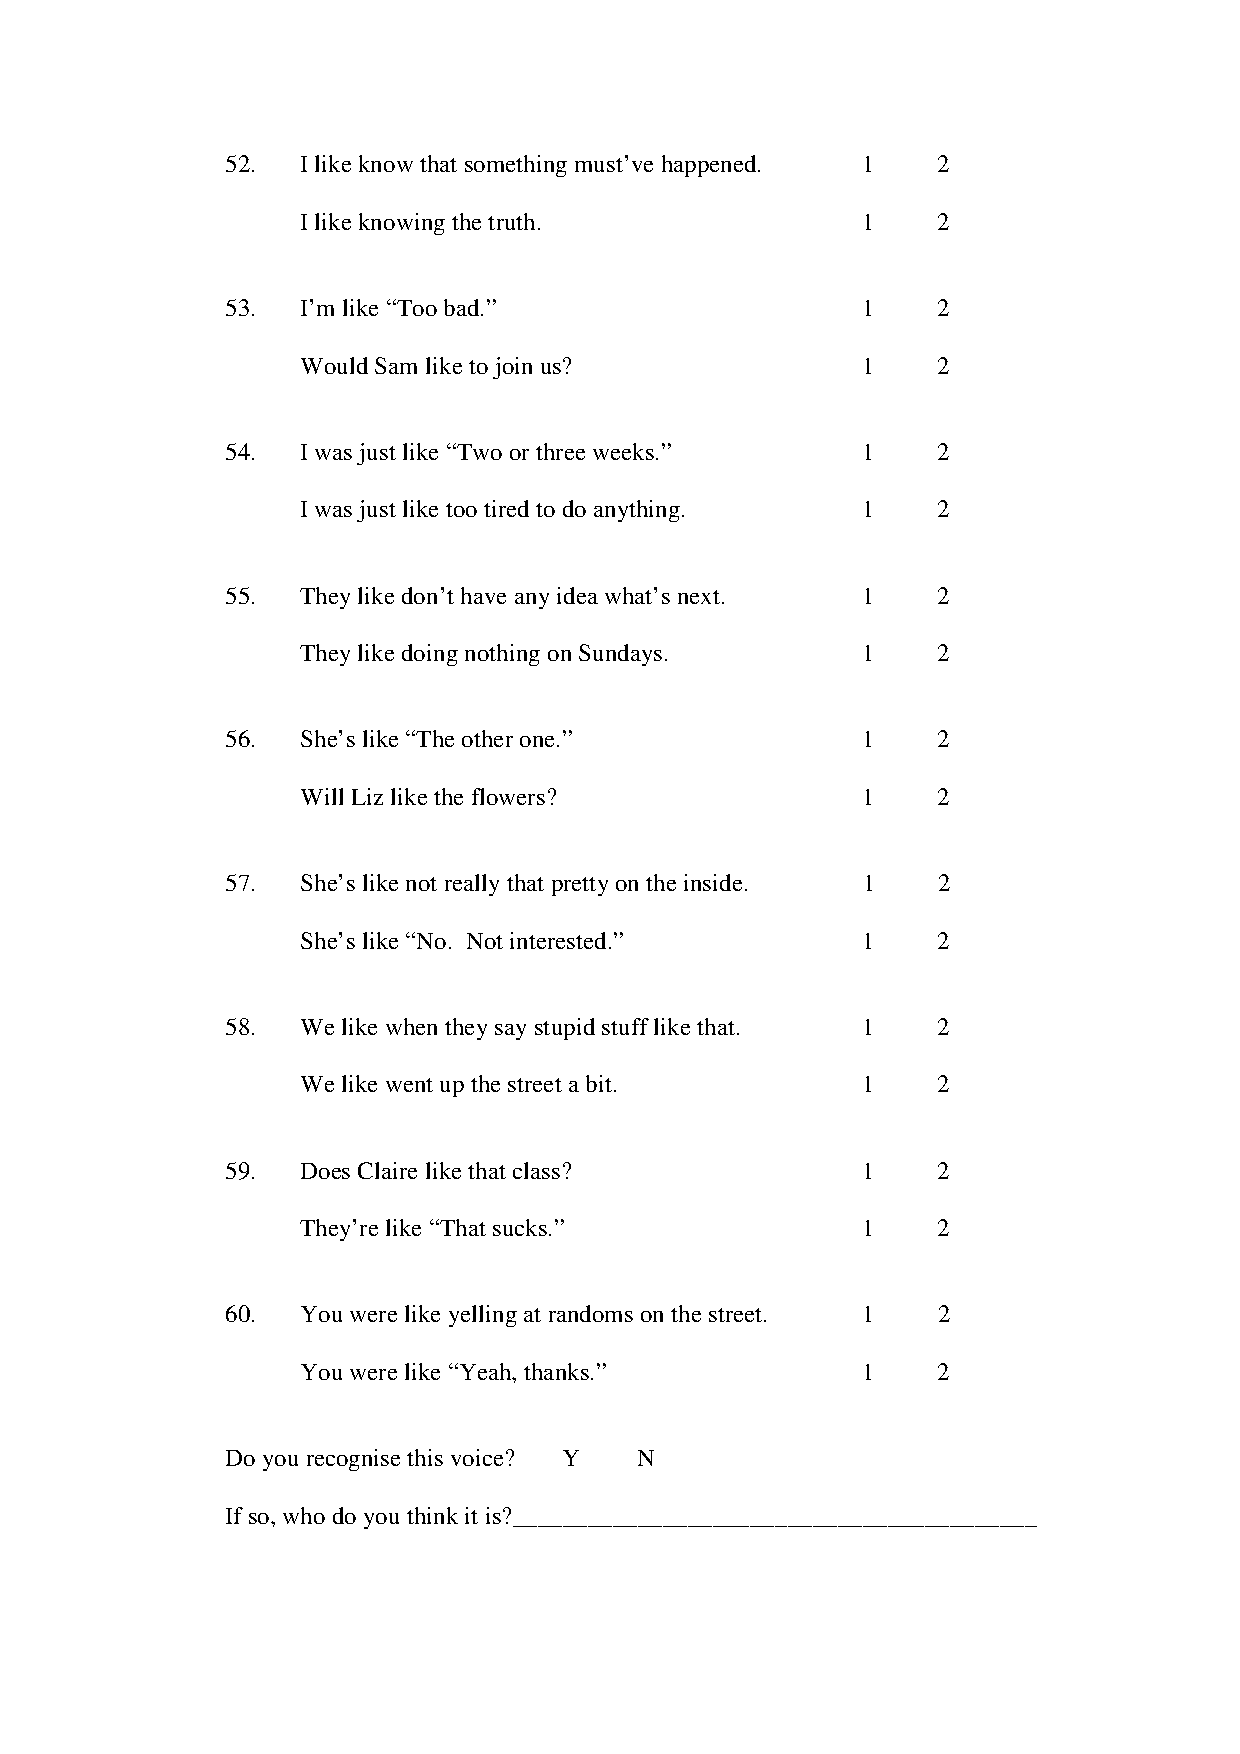
\includegraphics[width=5in]{images/Exp2page7.pdf}
			\label{x2p7}
\end{figure}



\begin{figure}
	\centering
		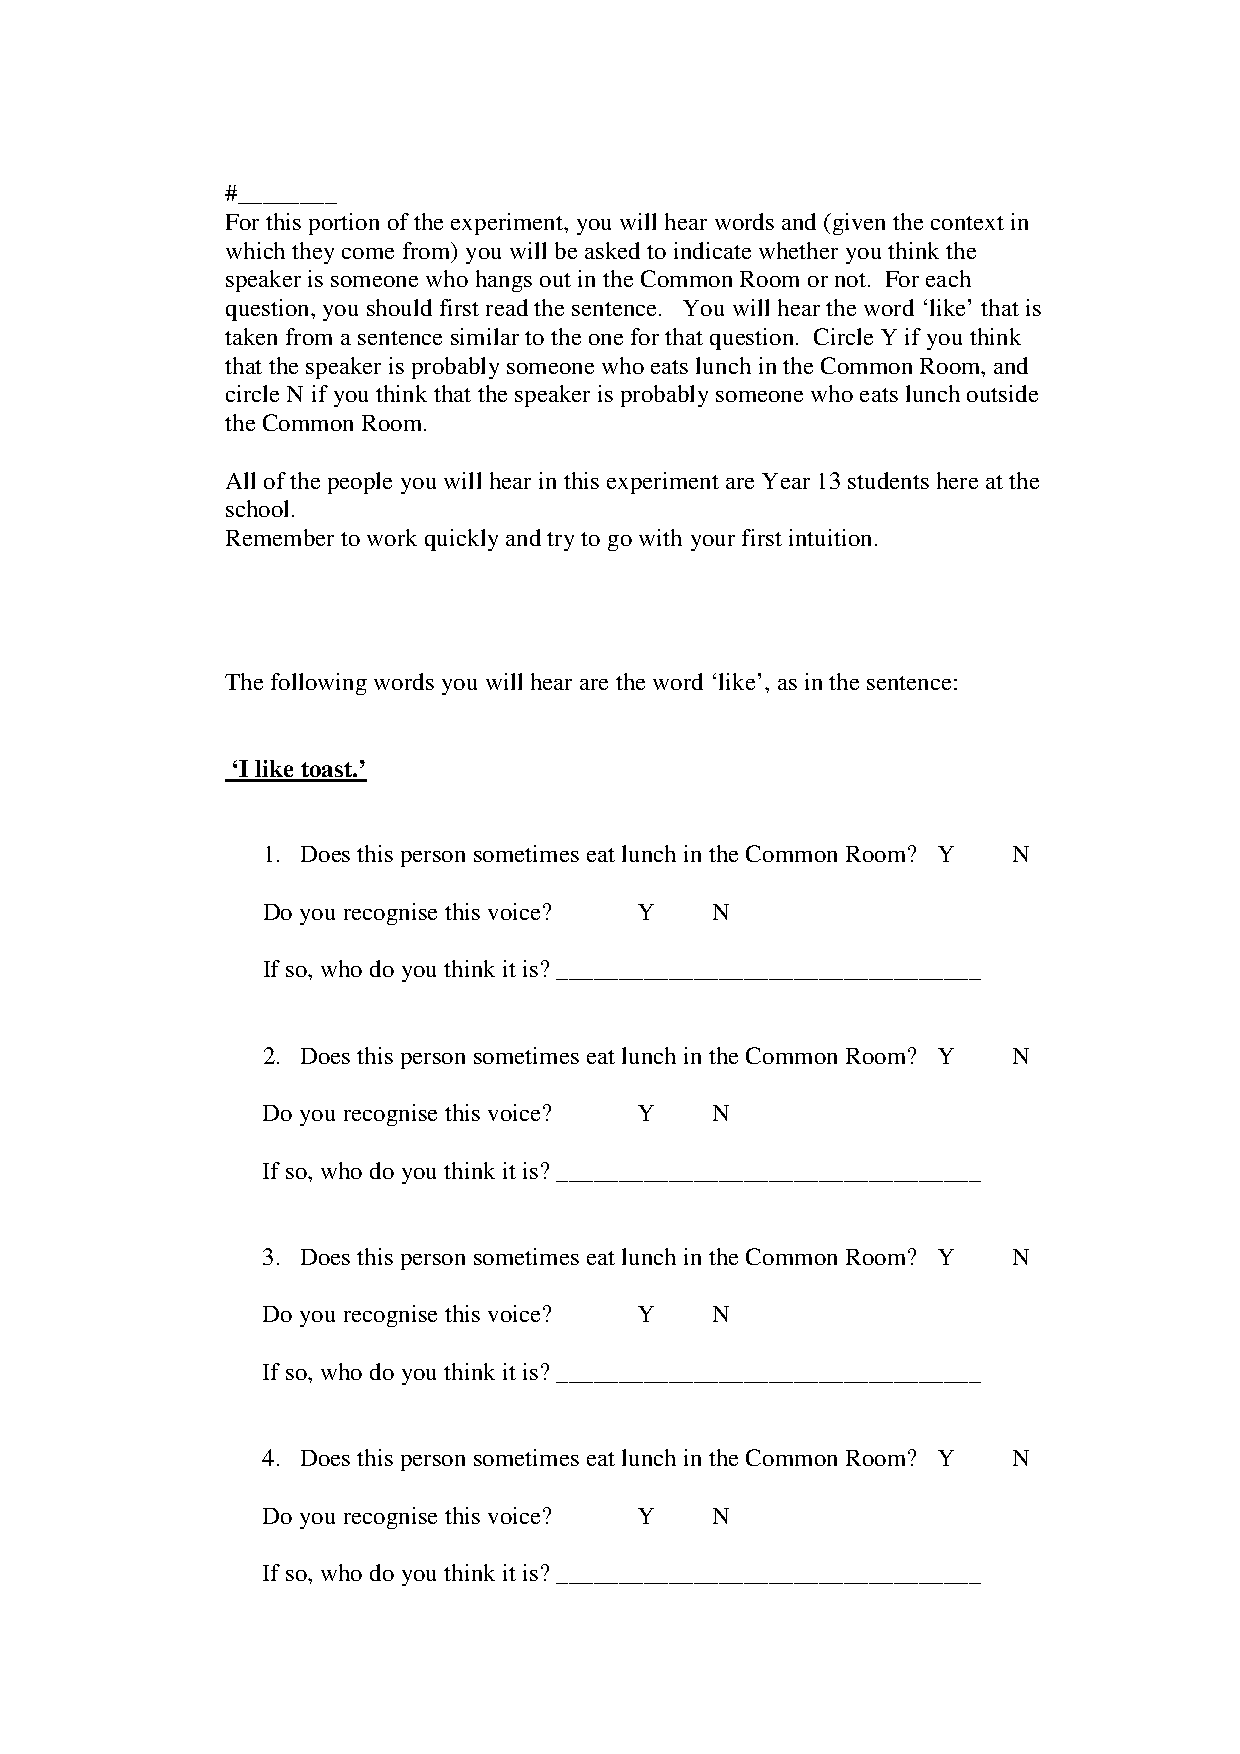
\includegraphics[width=5in]{images/Exp3page1.pdf}
		\caption{Answersheet for Experiment 3}
			\label{x3p1}
\end{figure}

\begin{figure}
	\centering
		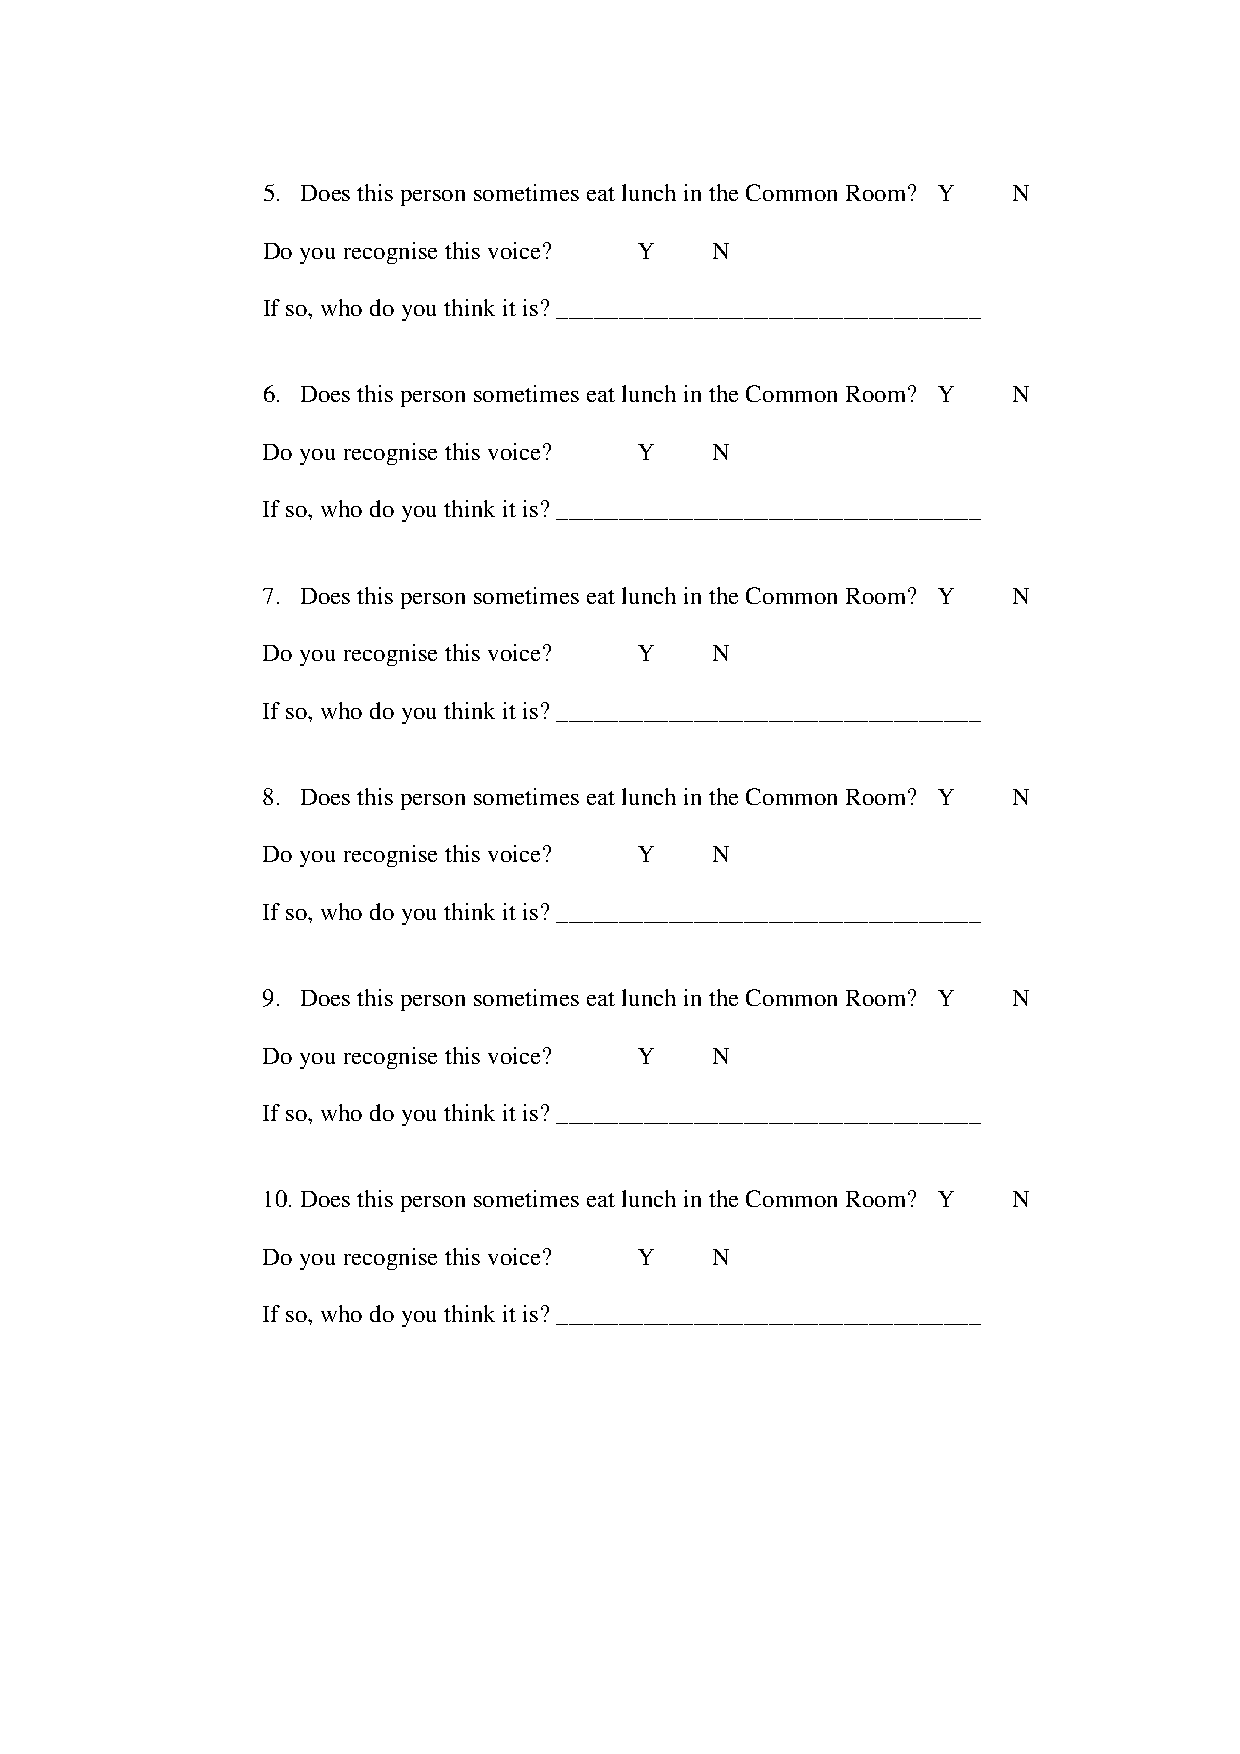
\includegraphics[width=5in]{images/Exp3page2.pdf}
		\label{x3p2}
\end{figure}

\begin{figure}
	\centering
		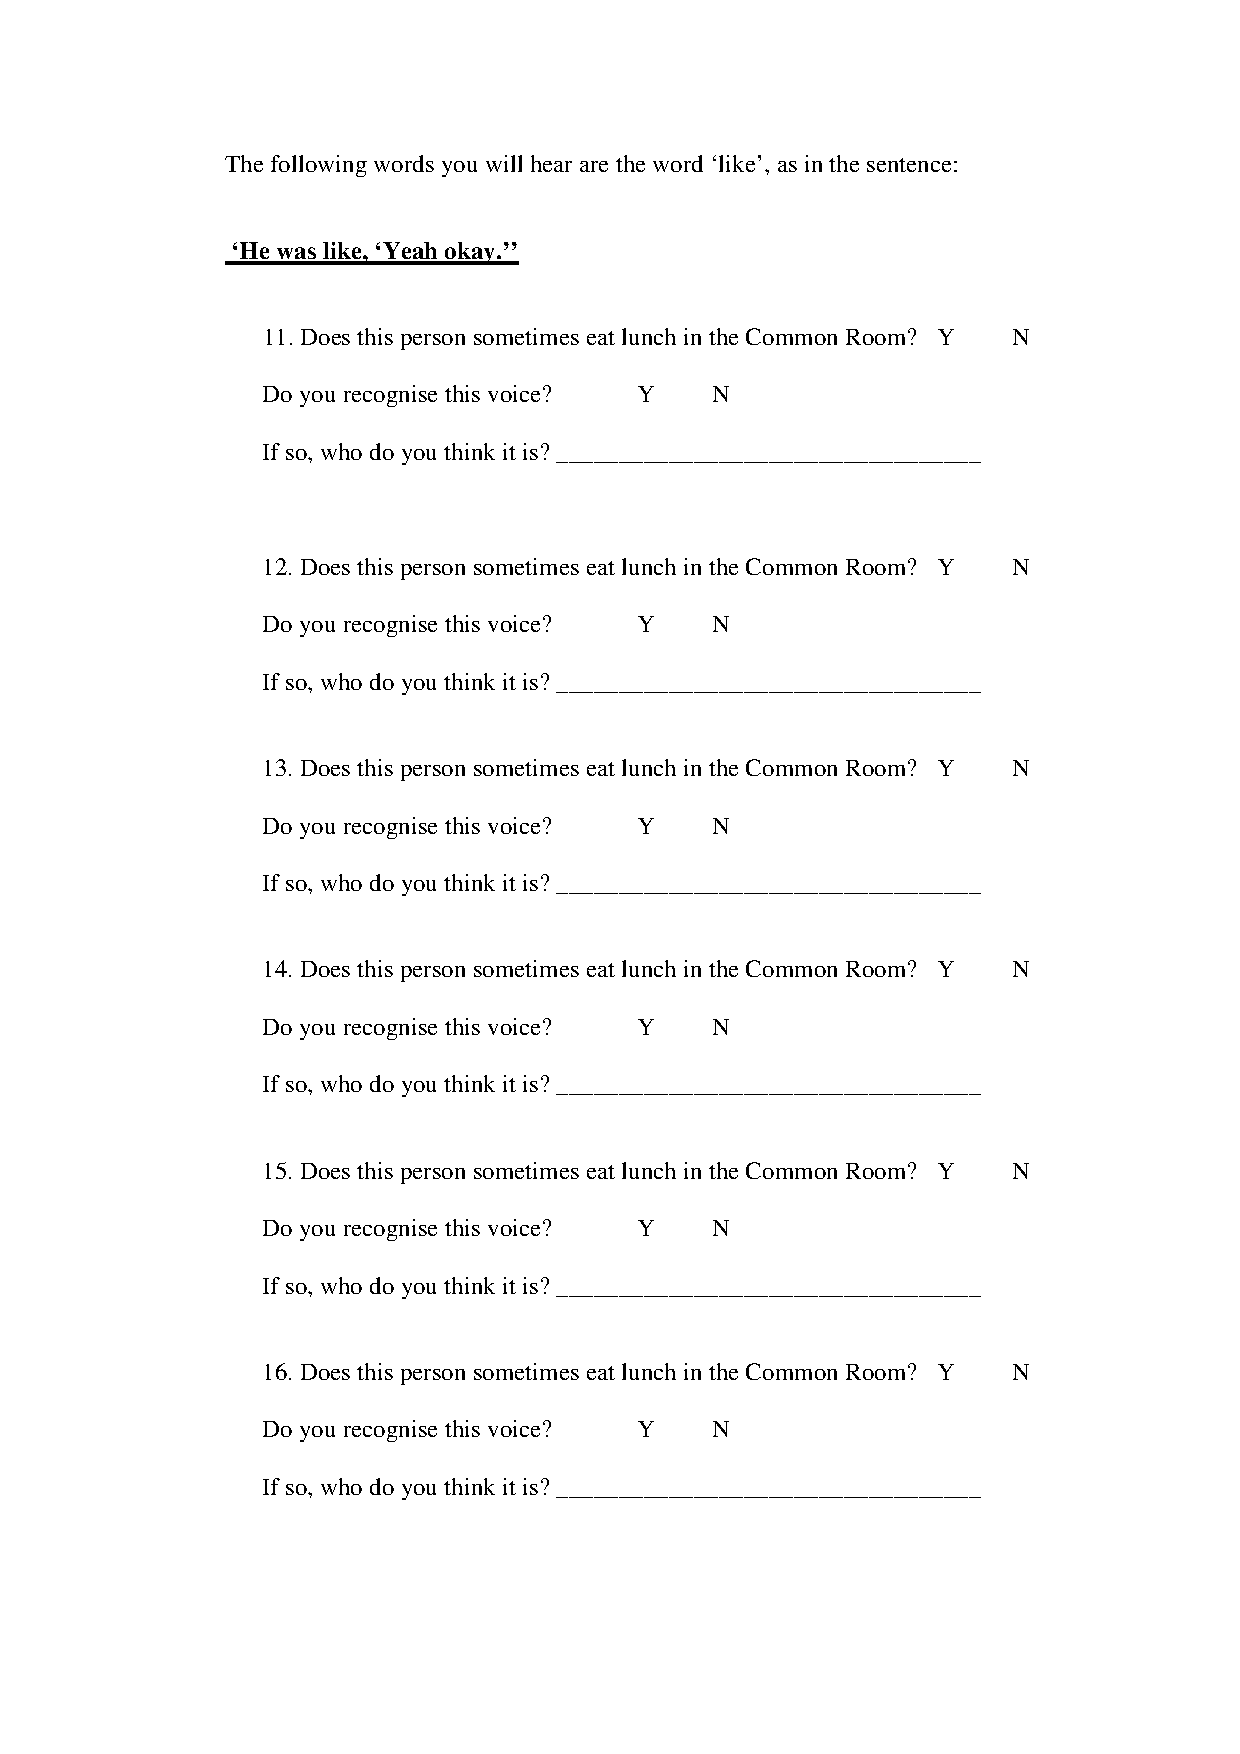
\includegraphics[width=5in]{images/Exp3page3.pdf}
		\label{x3p3}
\end{figure}

\begin{figure}
	\centering
		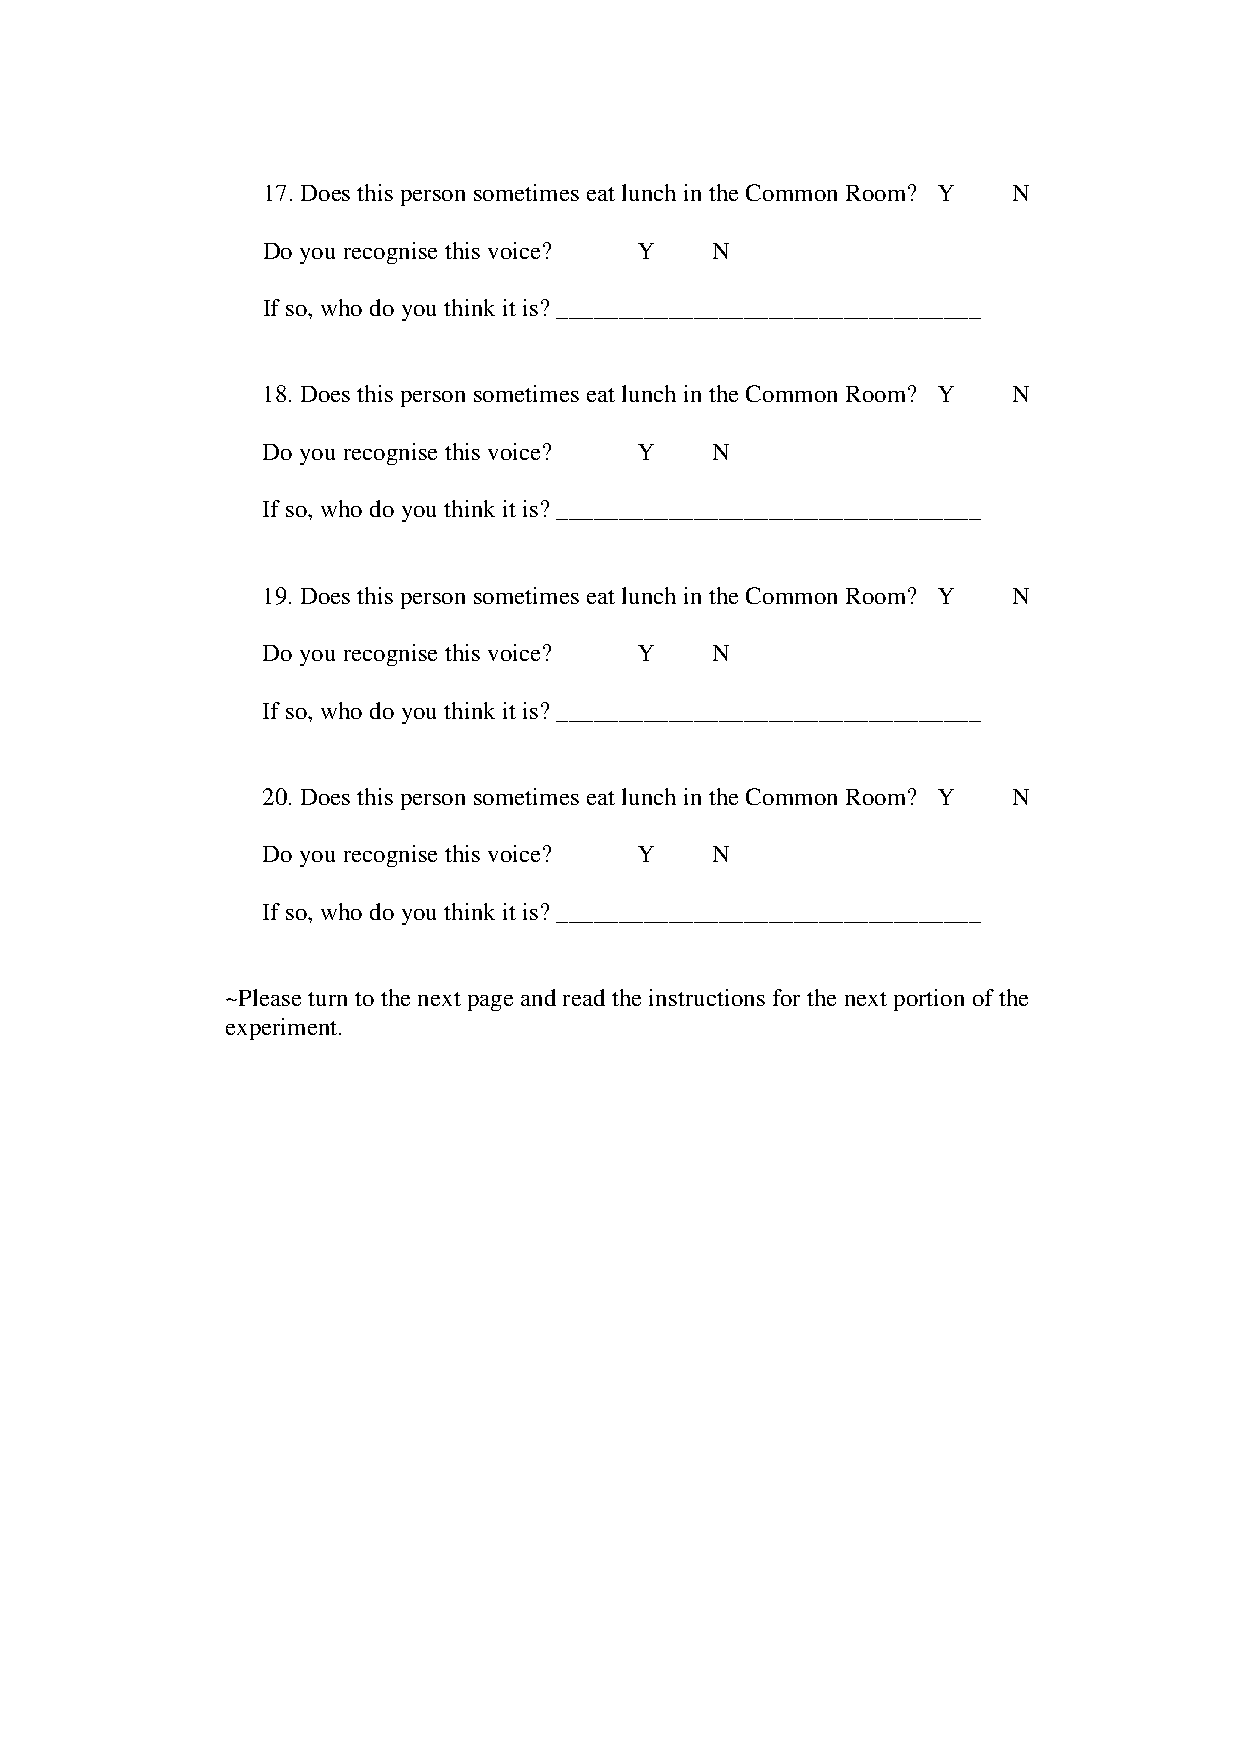
\includegraphics[width=5in]{images/Exp3page4.pdf}
		\label{x3p4}
\end{figure}

\begin{figure}
	\centering
		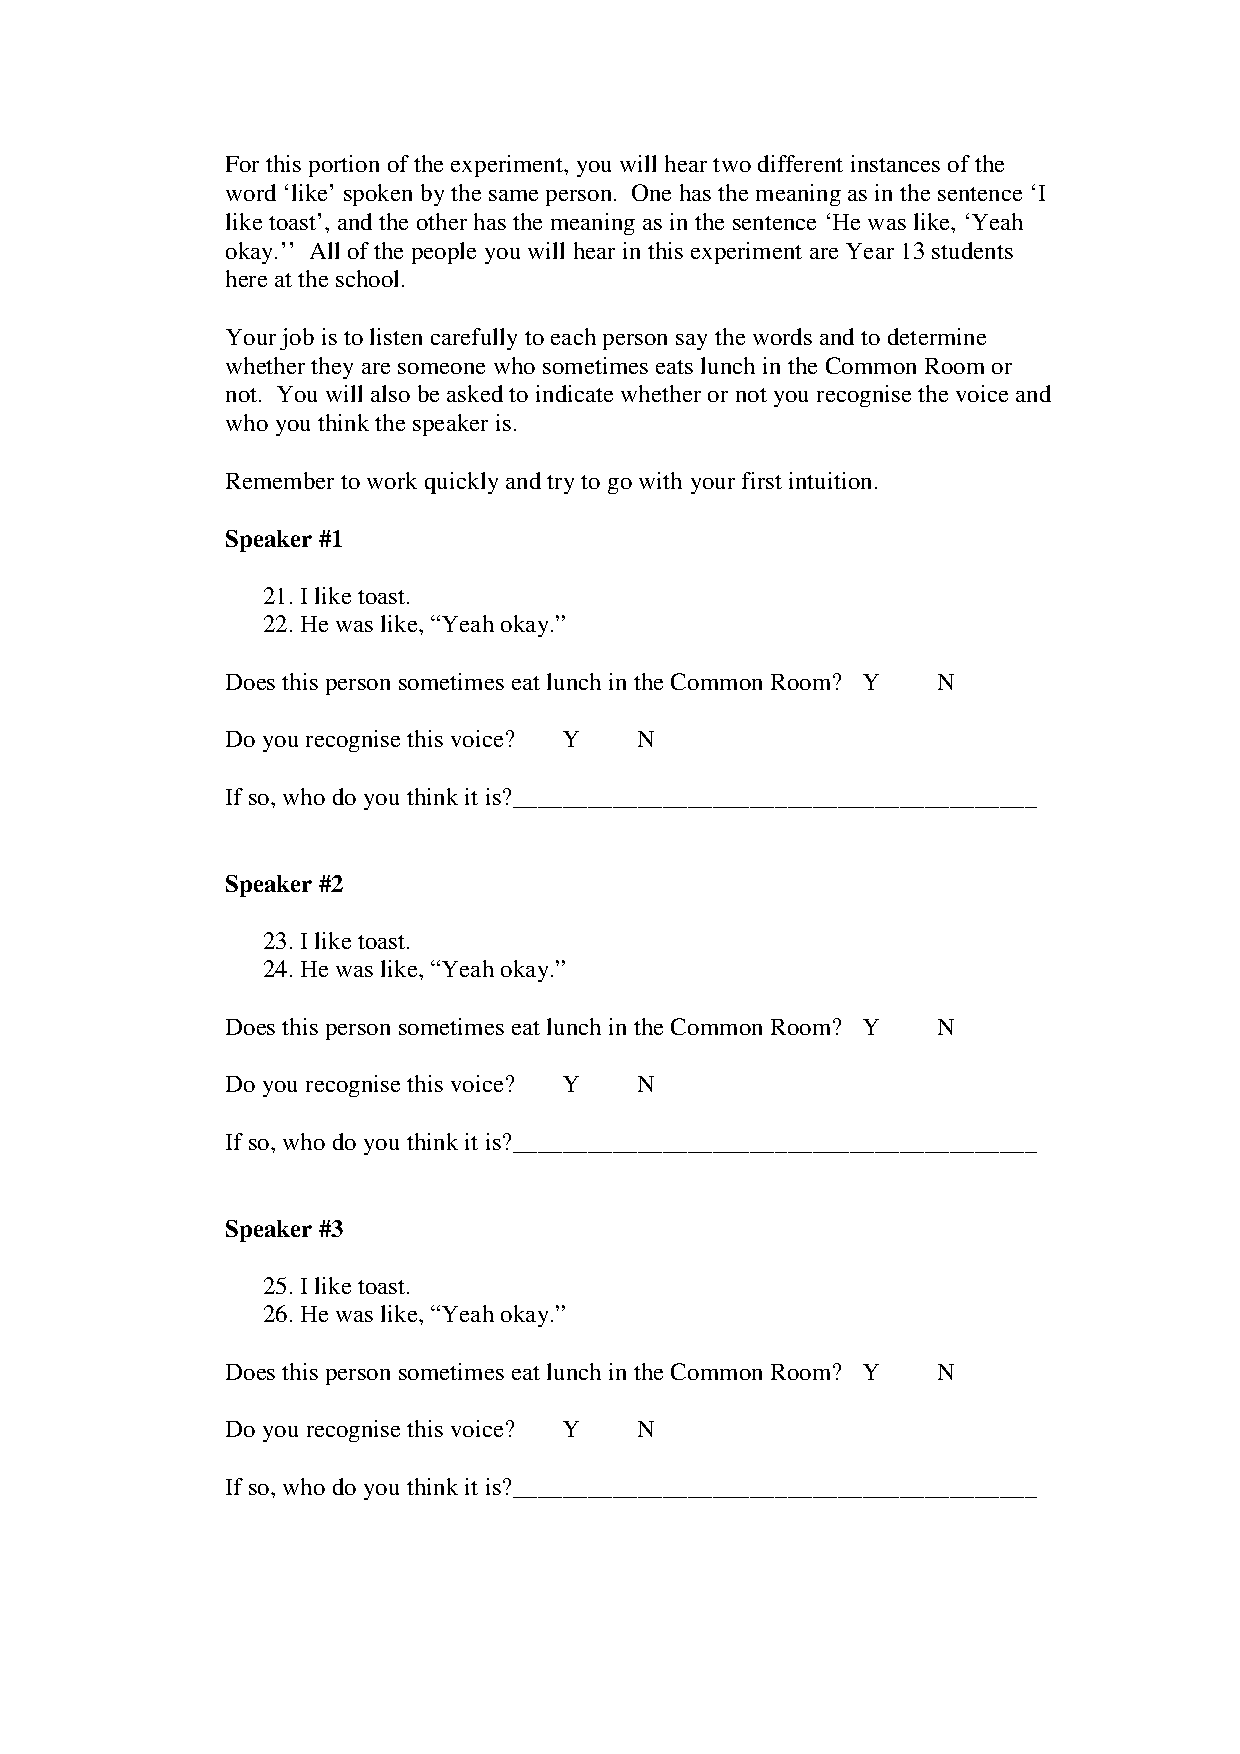
\includegraphics[width=5in]{images/Exp3page5.pdf}
		\label{x3p5}
\end{figure}

\begin{figure}
	\centering
		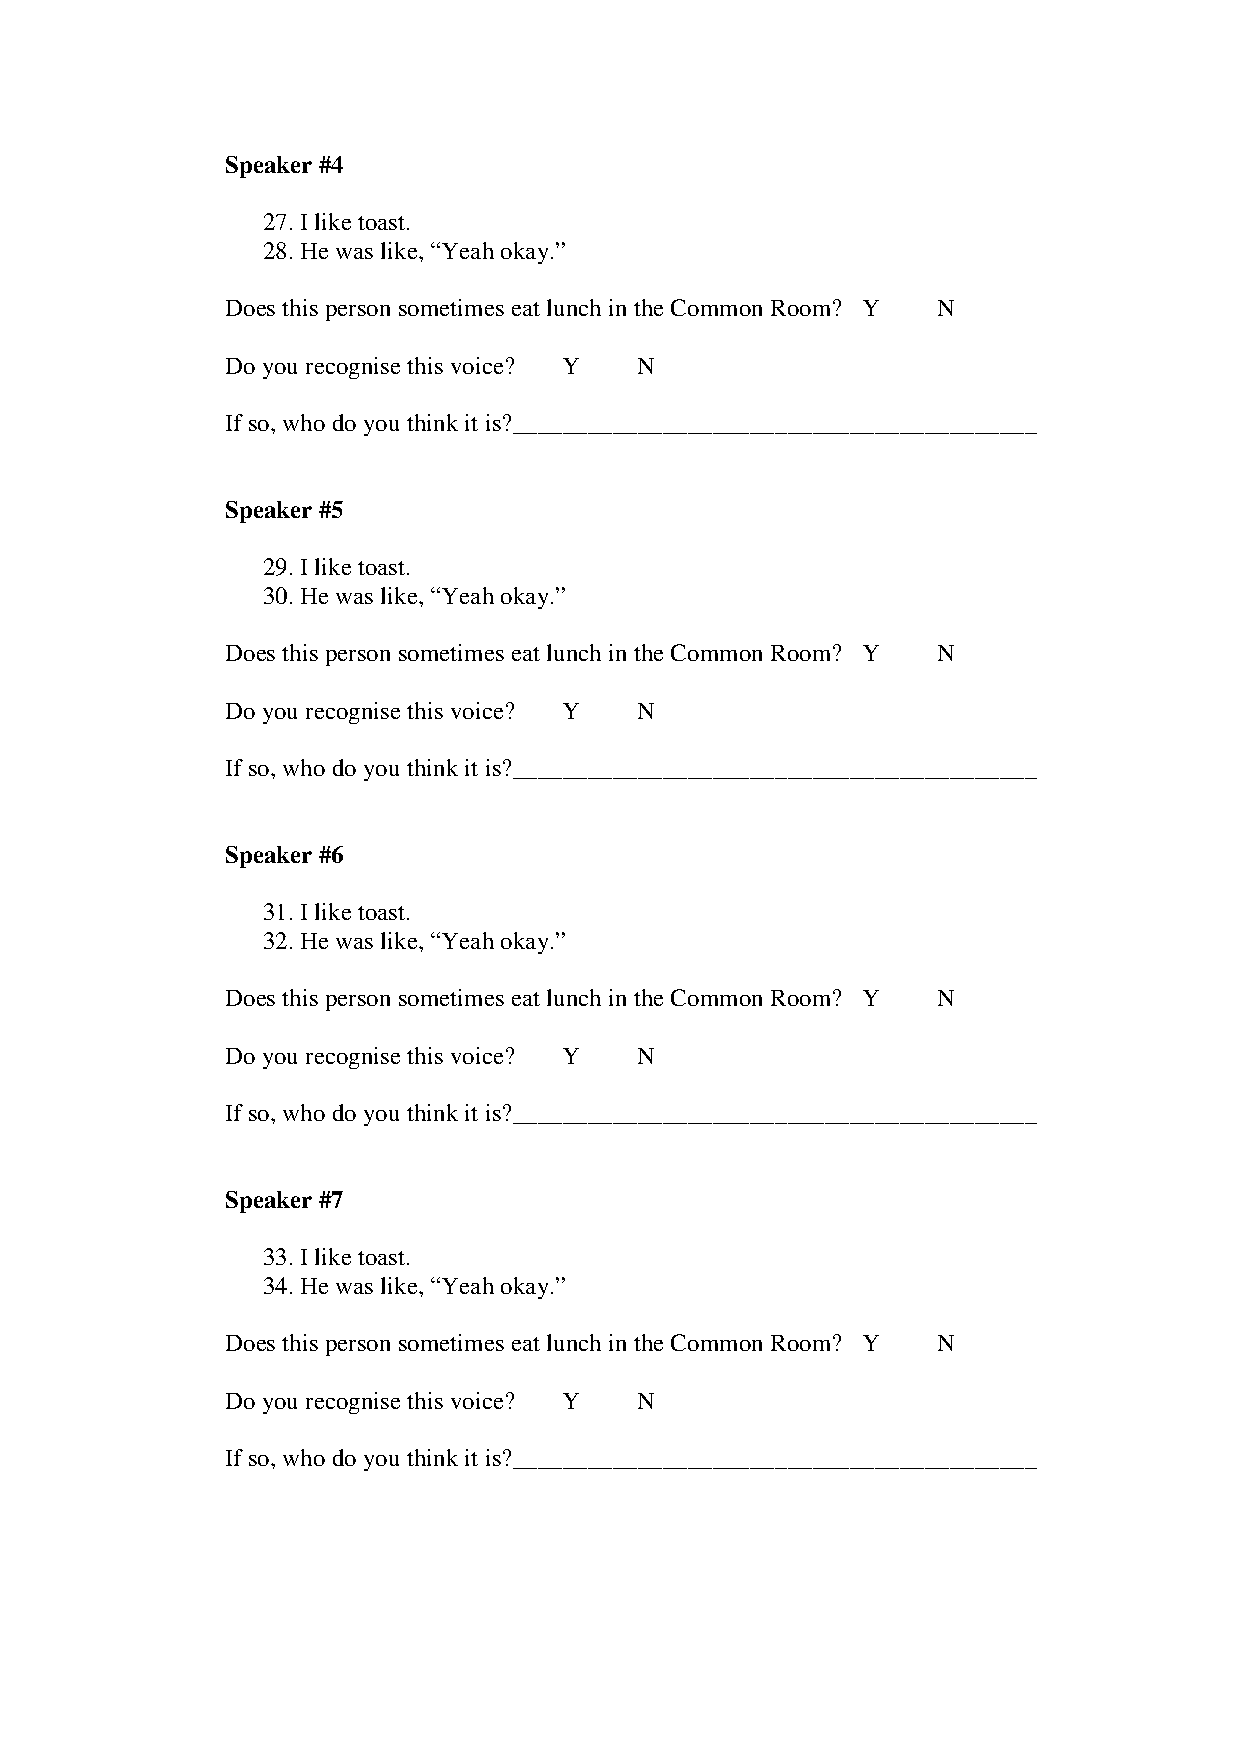
\includegraphics[width=5in]{images/Exp3page6.pdf}
		\label{x3p6}
\end{figure}

\begin{figure}
	\centering
		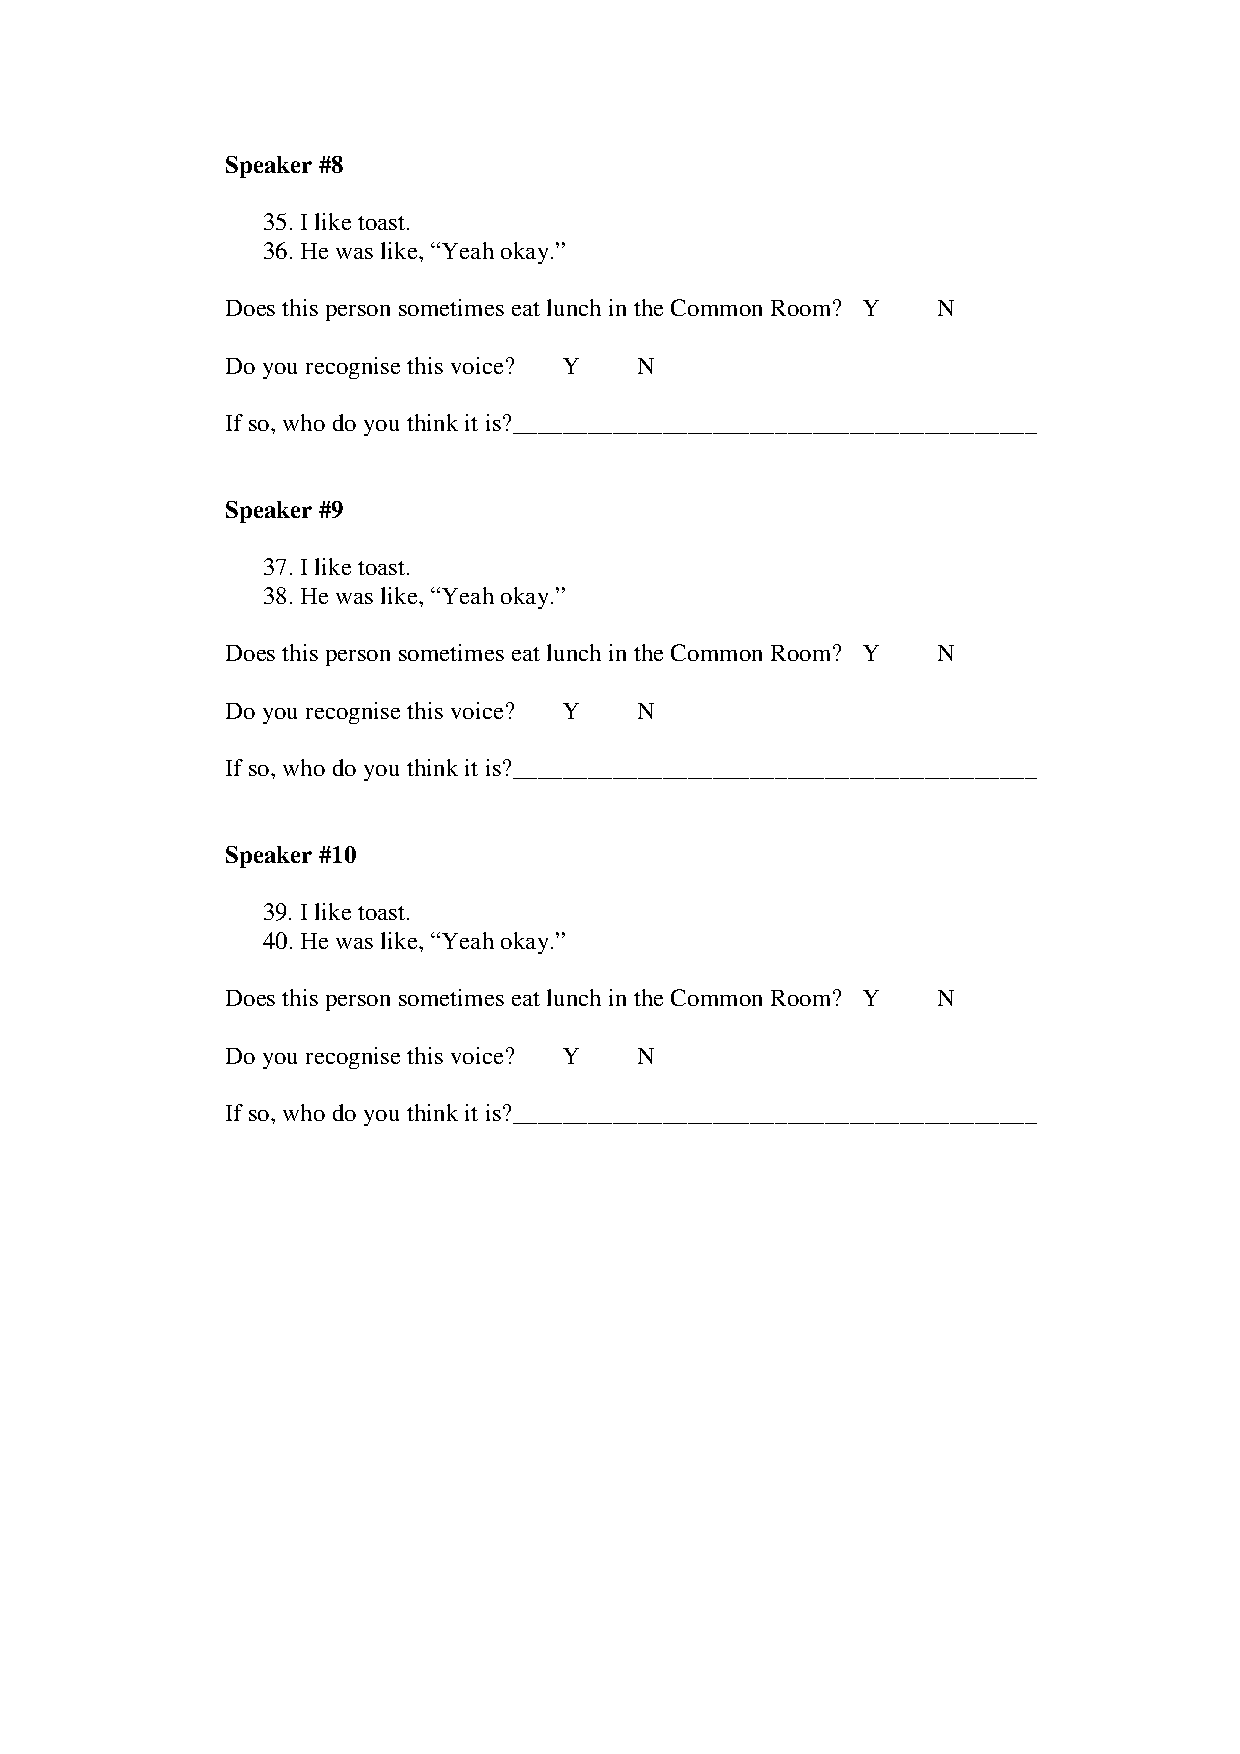
\includegraphics[width=5in]{images/Exp3page7.pdf}
		\label{x3p7}
\end{figure}



\begin{figure}[htbp]
	\centering
		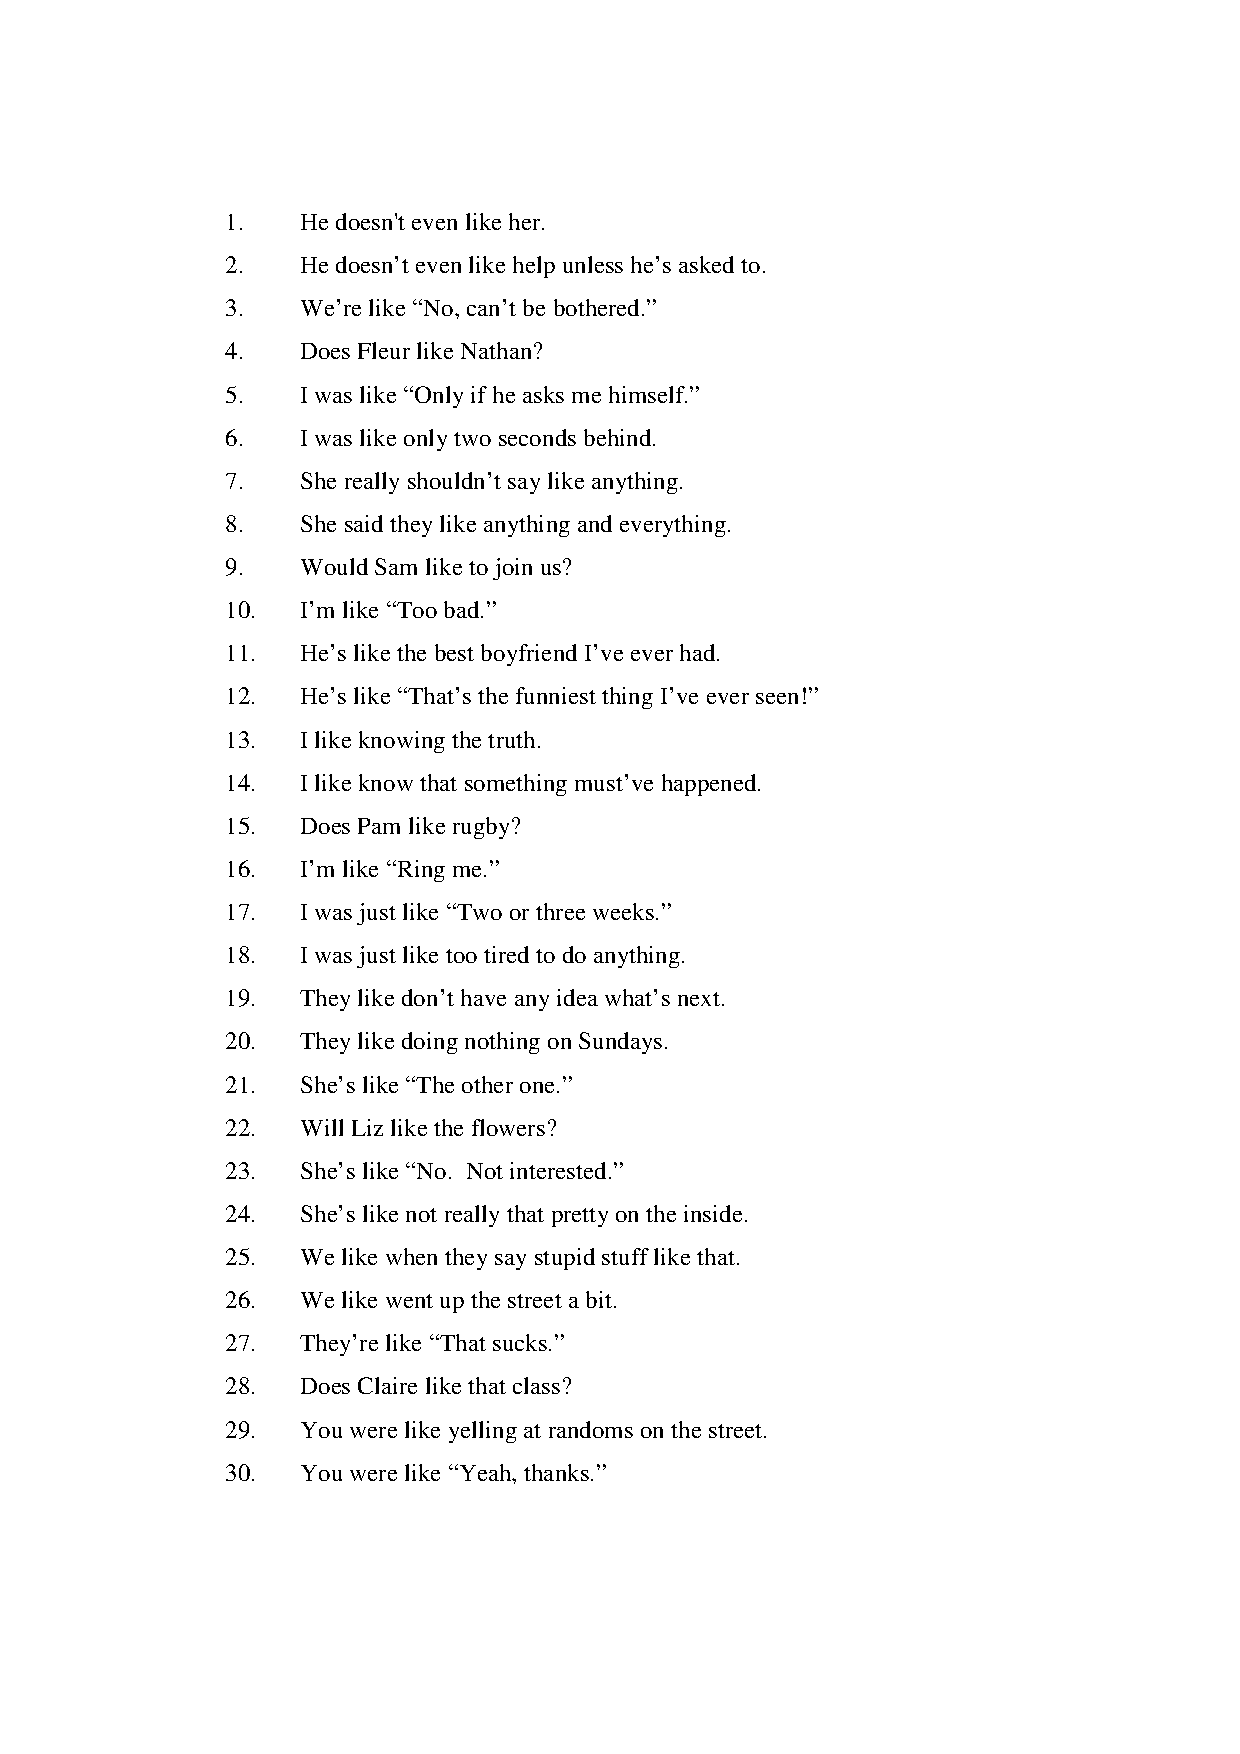
\includegraphics[width=5in]{images/ExpProductionTask.pdf}
	\caption{Production Task}
	\label{fig:ExpProductionTask}
\end{figure}




\begin{sidewaystable}[htbp]
\begin{center}
\resizebox{.9\textwidth}{!}{
\begin{tabular}{llllllllll}
  \lsptoprule
  
 num.	& (N)CR &	voice	& type1 &	type2&	person &	tense	& preced.	& token1 &	token2 \\
 \midrule
1	& CR	& Rose	   & d &	q	& match	& match	& match	& rose-Iwaslike1discp &	rose-Iwaslike1quote \\
2	&NCR	& Isabelle &	d &	q	& match	& match	& match	& isabelle-hewaslike1discp &	isabelle-hewaslike2quote \\
3	& CR	& Rose	   &g	&d 	   &match	& mismatch	& no info	& rose-it'slike1prep	& rose-itwaslike1discp \\
4	& CR	& Tracy	& d &	q	& mismatch & match	& likely	& tracy-he'slike1discp &	tracy-you'relike1quote \\
5	& NCR	& Isabelle &	q	& d 	& match	& mismatch & unlikely	& isabelle-shewasjustlike1quote & isabelle-she'slike1discp \\
6	& NCR	& Onya	& g	& d &	mismatch &	match	& no info	& onya-youlike1main	& onya-Ilike2discp \\
7	& CR	& Rose	& d &	q	& match	& mismatch & unlikely	& rose-itwaslike1discp	& rose-it'slike3quote \\
8	& CR	& Rachael	& d &	g &	match	& match	& match	& rachael-it'slike1discp & rachael-it'slike2prep \\
9	& NCR	& Onya & d & q & match & match & match & onya-she'slike1 & onya-she'slike1quote \\
10 & NCR & Isabelle &	d &	q	& match	& match	& match	& isabelle-shewaslike1discp	& isabelle-shewaslike1quote \\
11&	CR & Rose & g & d & mismatch	& match	& no info &	rose-Ilike1main & rose-theylike1discp \\
12 & CR & Tracy & d & q & match	& mismatch & unlikely & tracy-andtheywerelike2discp & tracy-andthey'relike1quote \\
13 & NCR & Onya & q & d & match & match & match & onya-they'relike1quote & onya2may-they'relike1 \\
14 & NCR & Isabelle & g & d & match	& match & match & isabelle-helike1main & isabelle-helike1discp \\
15 & CR & Tracy & g & d & mismatch & match & no info & tracy-Ilike1main & tracy-youlike1discp \\
16 & CR & Daphne & q & d & mismatch & match & likely & daphne-Iwaslike1quote & daphne-theywerelike1discp \\
17 & NCR & Isabelle & q & d & match & match & match & isabelle-hewaslike1quote & isabelle-hewaslike1discp \\
18 & NCR & Sarah & d & q & match & mismatch & likely & sarah-it'slike4discp	& sarah-itwaslike1quote \\
19 & CR	& Rose	& d & g & match &	match &	match &	rose-Iwaslike1discp & rose-Iwaslike1prep \\
20 & CR & Rachael & q & d & match &	match &	match &	rachael-it'sjustkindoflike1	& rachael-it'slike1discp \\
21 & NCR & Isabelle & q & d & match	& match	& match	& isabelle-shewaslike2quote	& isabelle-shewaslike1discp \\
22 & NCR & Onya & d & g &	mismatch & match & no info & onya-Ilike1discp	& onya-youlike1main  \\
23 & CR	& Rose	& d & q &	match &	mismatch & unlikely &	rose-itwaslike1discp &	rose-it'slike2quote \\
24 & NCR & Onya &	d &	q &	match &	match &	match	& onya2may-they'relike2	& onya-thegirlsarelike1quote \\
25 & CR	& Rose &	q &	d & match &	match &	match &	rose-Iwaslike2quote &	rose-Iwaslike1discp \\
26 & NCR & Onya &	q	& d &	match	& match	& match	& onya-wewerelike2 & onya-wewerelike3 \\
27 & NCR & Isabelle &	d &	g &	match	& match &	match &	isabelle-youlike1discp & isabelle-yalike1main \\
28 & CR &	Rose &	q &	d & match &	mismatch & likely &	rose-they'relike1quote	& rose-theywerelike \\
29 & CR & Tracy &	q	& d & match &	match &	match &	tracy-yourmum'slike1quote &	tracy-she'slike1discp \\
30 & CR &	Rose &	d &	q	& match	& match	& match	& rose-Iwaslike1discp & rose-Iwaslike1quote \\
31 & NCR & Onya	& d &	g	& mismatch & mismatch	& no info &	onya-Ilike3discp & onya-youlike1main \\ 
   \lspbottomrule 
\end{tabular}
}
\caption{The auditory stimuli played for each question in Experiment 1, listed by order played.}\label{tab:appenExp1stimuli}
\end{center}
\end{sidewaystable}	

\clearpage

\begin{table}[t] 
\begin{center}
 \resizebox{\textwidth}{!}{ 
\begin{tabular}{lllllllll}
  \lsptoprule
  
num. &	(N)CR &	voice	& type1	& type2	& token1 & token2	& context1	& context2 \\
 \midrule
	
1	& CR	& Rose	& g	& d	& rose-like3	& rose-discp1 & g &	d \\
2	& CR	& Rose	& q	& g	& rose-quote2	& rose-like4	& q	& g \\
3	& CR	& Rose	& d	& q	& rose-discp1	& rose-quote1	& q	& d \\
4	& CR	& Rose	& d	& g	& rose-discp5	& rose-like9	& d	& g \\
5	& CR	& Rose	& q	& g	& rose-quote4	& rose-like9	& g	& q \\
6	& CR	& Rose	& q	& d	& rose-quote2	& rose-discp2	& d	& q \\
7	& CR	& Rose	& g	& d	& rose-like10	& rose-discp6	& g	& d \\
8	& CR	& Rose	& g	& q	& rose-like3	& rose-quote1	& g	& q \\
9	& CR	& Rose	& q	& d	& rose-quote4	& rose-discp5	& q	& d \\
10	& CR	& Rose	& g	& d	& rose-like8	& rose-discp3 &	d	& g \\
11	& CR	& Rose	& g	& q	& rose-like8	& rose-quote3	& q	& g \\
12	& CR	& Rose	& d	& q	& rose-discp6	& rose-quote5	& q	& d \\
13	& CR	& Rose	& d	& g	& rose-discp2	& rose-like4	& g	& d \\
14	& CR	& Rose	& g	& q	& rose-like10	& rose-quote5	& q	& g \\
15	& CR	& Rose	& d	& q	& rose-discp3	& rose-quote3	& d	& q \\
16	& NCR	& Meredith	& g	& d	& meredith-like1main	& meredith-like1discp	& d	& g \\
17	& NCR	& Meredith	& g	& q	& meredith-like5main	& meredith-like5quote	& g	& q \\
18	& NCR	& Meredith	& q	& d	& meredith-like2quote	& meredith-like2discp	& d	& q \\
19	& NCR	& Meredith	& d	& g	& meredith-like4discp	& meredith-like4main	& d	& g \\
20	& NCR	& Meredith	& g	& q	& meredith-like1main	& meredith-like1quote	& g	& q \\
21	& NCR	& Meredith	& d	& q	& meredith-like1discp	& meredith-like1quote	& d	& q \\
22	& NCR	& Meredith	& g	& d	& meredith-like5main	& meredith-like5discp	& g	& d \\
23	& NCR	& Meredith	& q	& g	& meredith-like2quote	& meredith-like2main	& g	& q \\
24	& NCR	& Meredith	& q	& d	& meredith-like4quote	& meredith-like4discp	& q	& d \\
25	& NCR	& Meredith	& g	& d	& meredith-like3main	& meredith-like3discp	& d	& g \\
26	& NCR	& Meredith	& g	& q	& meredith-like3main	& meredith-like3quote	& q	& g \\
27	& NCR	& Meredith	& d	& q	& meredith-like3discp	& meredith-like3quote	& d	& q \\
28	& NCR	& Meredith	& d	& g	& meredith-like2discp	& meredith-like2main	& g	& d \\
29	& NCR	& Meredith	& q	& g	& meredith-like4quote	& meredith-like4main	& q	& g \\
30	& NCR	& Meredith	& d	& q	& meredith-like5discp	& meredith-like5quote	& q	& d \\
   \lspbottomrule
        &      &     	&   	&   	& \hspaceThis{meredith-like2discp}& \hspaceThis{meredith-like2discp}&           \\
   
	\end{tabular}
}
	\caption{The auditory stimuli played for each question in Experiment 2, listed by order played (1-30).}\label{tab:appenExp2stimuli}
	\end{center}
\end{table}	



\begin{table}[t]
\begin{center}
 \resizebox{\textwidth}{!}{ 
\begin{tabular}{lllllllll}
  \lsptoprule
  
num. &	(N)CR &	voice	& type1	& type2	& token1 & token2	& context1	& context2 \\
 \midrule
 
31	& CR	& Tracy	& d	& g	& tracy-discp1	& tracy-like1	& g	& d \\
32	& CR	& Tracy	& q	& g	& tracy-quote1	& tracy-like1	& g	& q \\
33	& CR	& Tracy	& d	& q	& tracy-discp2	& tracy-quote2	& d	& q \\
34	& CR	& Tracy	& g	& d	& tracy-like4	& tracy-discp4	& d	& g \\
35	& CR	& Tracy	& q	& g	& tracy-quote3	& tracy-like3	& q	& g \\
36	& CR	& Tracy	& q	& d	& tracy-quote1	& tracy-discp1 &	q &	d \\
37	& CR	& Tracy	& d	& g	& tracy-discp3	& tracy-like3	& d	& g \\
38	& CR	& Tracy	& g	& q	& tracy-like4	& tracy-quote4	& g	& q \\
39	& CR	& Tracy	& q	& d	& tracy-quote5	& tracy-discp5	& q	& d \\
40	& CR	& Tracy	& d	& g	& tracy-discp5	& tracy-like5	& g	& d \\
41	& CR	& Tracy	& g	& q	& tracy-like2	& tracy-quote2	& q	& g \\
42	& CR	& Tracy	& q	& d	& tracy-quote3	& tracy-discp3	& d	& q \\
43	& CR	& Tracy	& g	& d	& tracy-like2	& tracy-discp2	& g	& d \\
44	& CR	& Tracy	& q	& g	& tracy-quote5	& tracy-like5	& q	& g \\
45	& CR	& Tracy	& d	& q	& tracy-discp4	& tracy-quote4	& q	& d \\
46	& NCR	& Onya	& d	& g	& onya-discp1	& onya- like6	& g	& d \\
47	& NCR	& Onya	& q	& g	& onya-quote1	& onya- like6	& g	& q \\
48	& NCR	& Onya	& d	& q	& onya-discp2	& onya-quote2	& d	& q \\
49	& NCR	& Onya	& g	& d	& onya- like9	& onya-discp4	& d	& g \\
50	& NCR	& Onya	& g	& q	& onya- like7	& onya-quote2	& g	& q \\
51	& NCR	& Onya	& q	& d	& onya-quote1	& onya-discp1	& q	& d \\
52	& NCR	& Onya	& d	& g	& onya-discp5	& onya- like10	& d	& g \\
53	& NCR	& Onya	& g	& q	& onya- like9	& onya-quote4	& q	& g \\
54	& NCR	& Onya	& d	& q	& onya-discp4	& onya-quote4	& q	& d \\
55	& NCR	& Onya	& d	& g	& onya-discp3	& onya- like8	& d	& g \\
56	& NCR	& Onya	& q	& g	& onya-quote3	& onya- like8	& q	& g \\
57	& NCR	& Onya	& q	& d	& onya-quote5 &	onya-discp5	& d	& q \\
58	& NCR	& Onya	& g	& d	& onya- like7	& onya-discp2	& g	& d \\
59	& NCR	& Onya	& q	& g	& onya-quote5	& onya- like10	& g	& q \\
60	& NCR	& Onya	& q	& d	& onya-quote3	& onya-discp3	& d	& q \\
   \lspbottomrule
        &      &     	&   	&   	& \hspaceThis{meredith-like2discp}& \hspaceThis{meredith-like2discp}&           \\

   
	\end{tabular}
}
	\caption{The auditory stimuli played for each question in Experiment 2, listed by order played.  (31-60)}\label{tab:appenExp2stimuli3160}
	\end{center}
\end{table}	



\clearpage


\begin{table}[htbp]
\begin{center}
\resizebox{\textwidth}{!}{
\begin{tabular}{llllllll}
  \lsptoprule
  
task & num. & (N)CR &	voice	& type1	& type2	& token1 & token2	\\
 \midrule
 
 1 & 1 & CR & Anita & g & na & anita-like1 & na \\
 1 & 2 & NCR & Vanessa & g & na & vanessa-like1 & na \\
 1 & 3 & NCR & Onya & g & na & onya-like6 & na \\
 1 & 4 & CR & Rose & g & na & rose-like9 & na \\
 1 & 5 & NCR & Meredith & g & na & meredith-like1 & na \\
 1 & 6 & CR & Rachel & g & na & rachel-like1 & na \\
 1 & 7 & CR & Tracy & g & na & tracy-like2 & na \\
 1 & 8 & NCR & Isabelle & g & na & isabelle-like2 & na \\
 1 & 9 & CR & Betty & g & na & betty-like1 & na \\
 1 & 10 & NCR & Sarah & g & na & sarah-like1 & na \\
 2 & 11 & NCR & Isabelle & q & na & isabelle-quote5 & na \\
 2 & 12 & NCR & Onya & q & na & onya-quote4 & na \\
 2 & 13 & CR & Rose & q & na & rose-quote2 & na \\
 2 & 14 & NCR & Sarah & q & na & sarah-quote1 & na \\
 2 & 15 & CR & Rachel & q & na & rachael-quote1 & na \\
 2 & 16 & CR & Betty & q & na & betty-quote1 & na \\
 2 & 17 & NCR & Vanessa & q & na & vanessa-quote1 & na \\
 2 & 18 & CR & Anita & q & na & anita-quote2 & na \\
 2 & 19 & NCR & Meredith & q & na & meredith-quote6 & na \\
 2 & 20 & CR & Tracy & q & na & tracy-quote1 & na \\
 3 & 21--22 & CR & Betty & g & q & betty-like1 & betty-quote1 \\
 3 & 23--24 & NCR & Isabelle & g & q & isabelle-like2 & isabelle-quote5 \\
 3 & 25--26 & CR & Rose & g & q & rose-like9 & rose-quote2 \\
 3 & 27--28 & NCR & Onya & g & q & onya-like6 & onya-quote4 \\
 3 & 29--30 & CR & Rachel & g & q & rachel-like1 & rachel-quote1 \\
 3 & 31--32 & NCR & Sarah & g & q & sarah-like1 & sarah-quote1 \\
 3 & 33--34 & CR & Tracy & g & q & tracy-like2 & tracy-quote1 \\
 3 & 35--36 & NCR & Vanessa & g & q & vanessa-like1 & vanessa-quote1 \\
 3 & 37--38 & CR & Anita & g & q & anita-like1 & anita-quote2 \\
 3 & 39--40 & NCR & Meredith & g & q & meredith-like1 & meredith-quote6 \\
 
    \lspbottomrule
   
	\end{tabular}
}
	\caption{The auditory stimuli played for each question in Experiment 3, listed by order played.}\label{tab:appenExp3stimuli}
	\end{center}
\end{table}
\newpage
\thispagestyle{empty}
\mbox{}
\chapter{Perception experiment data}\label{appen:percdata}

Participants' responses are displayed in Tables \ref{tab:percExp1responsesqd} and \ref{tab:percExp1responsesgd} for Experiment 1, Tables \ref{tab:percExp2responsesqd}-\ref{tab:percExp2responsesgd} for Experiment 2, and Tables \ref{tab:appenpercExp3Task1responses}-\ref{tab:appenpercExp3Task3responses} for Experiment 3.  





\begin{table}[htbp]
\begin{center}
\resizebox{\textwidth}{!}{
\begin{tabular}{ld{5}d{5}d{5}}
   \lsptoprule
   feature & \multicolumn{1}{c}{CR girl} &  \multicolumn{1}{c}{NCR girl} & \multicolumn{1}{c}{CR and NCR} \\
   questions comparing & \multicolumn{1}{c}{quote$-$dp} &  \multicolumn{1}{c}{quote$-$dp} &  \multicolumn{1}{c}{quote$-$dp} \\
  \midrule
  total number subjects & 23 & 19 & 42 \\
  total questions answered & 916 & 774 & 1690 \\
  total 1st token labeled as quote & 465 & 383 & 848 \\
  quote first on sheet & 278 & 231 &  509 \\
  1st token's context more likely & 110 & 73 &  183 \\
  1st and 2nd tokens' context matched & 271 & 242 & 513 \\
  1st token's context less likely & 84 & 68 & 152 \\
  1st token mean EucD & 1.5930 & 1.5400  & 1.5690 \\
  2nd token mean EucD & 1.6180 & 1.6720 & 1.6430 \\
  mean EucD diff. (Bark) & -0.02538  & -0.13280 &  -0.07388 \\
  1st token mean nuc F2 (Bark) & 11.25  & 11.19 & 11.23 \\
  2nd token mean nuc F2 (Bark) & 11.49 & 11.45 & 11.47 \\
  mean nuc F2 diff. (Bark) & -0.2379 & -0.2554  & -0.2458 \\
 	1st token mean duration ratio & 0.33900  & 0.32670 & 0.33350 \\
 	2nd token mean duration ratio & 0.35020  & 0.34520  & 0.34790 \\
  mean duration ratio diff. & -0.01120  & -0.01844 &  -0.01447 \\
  1st token $[$k$]$ present, 2nd token $[$k$]$ absent & 93  & 84  & 177\\
  1st token $[$k$]$ absent, 2nd token $[$k$]$ present & 74  & 65  & 139 \\
  $[$k$]$ present for both tokens & 118 & 83 & 201 \\
  $[$k$]$ absent for both tokens & 180  & 151 & 331 \\
    \lspbottomrule
    
  
  \end{tabular}
}
\caption{Characteristics of quote$-$dp questions in Experiment 1 where the first token was identified as the quotative, by whether the participant was in a CR or a NCR group.}\label{tab:percExp1responsesqd}
\end{center}
\end{table}	



\begin{table}[htbp]
\begin{center}
\resizebox{\textwidth}{!}{
\begin{tabular}{ld{6}d{8}d{8}}
   \lsptoprule
   feature & \multicolumn{1}{c}{CR} &   \multicolumn{1}{c}{NCR} & \multicolumn{1}{c}{CR and NCR} \\
   questions comparing & \multicolumn{1}{c}{gram$-$dp} & \multicolumn{1}{c}{gram$-$dp} & \multicolumn{1}{c}{gram$-$dp} \\
  \midrule
  total number subjects & 23  & 19 & 42 \\
  total questions answered & 435  & 371 & 806 \\
  total 1st token labeled as gram & 235  & 197 & 432 \\
  gram first on sheet &  179 & 158 &  337 \\
  1st token mean EucD & 1.1450  & 1.1750 & 1.1580 \\
  2nd token mean EucD &  2.1720 & 2.3090 & 2.2350 \\
  mean EucD diff. (Bark) &  -1.0270   & -1.1350 &  -1.0760 \\
  1st token mean nuc F2 (Bark) & 11.610 & 11.680 & 11.640 \\
  2nd token mean nuc F2 (Bark) & 11.180  & 11.150 & 11.170 \\
  mean nuc F2 diff. (Bark) &  0.4210 & 0.5324 & 0.4718 \\
 	1st token mean duration ratio &  0.6032 &  0.5812 & 0.5918  \\
 	2nd token mean duration ratio &  0.5878 & 0.6098 &  0.5992 \\
  mean duration ratio diff. &  0.0017 &  -0.004056  & -0.0009248 \\
  1st token $[$k$]$ present, 2nd token $[$k$]$ absent & 35  & 35  & 70 \\
  1st token $[$k$]$ absent, 2nd token $[$k$]$ present &  29  & 28  & 57 \\
  $[$k$]$ present for both tokens &  90 & 69  & 159  \\
  $[$k$]$ absent for both tokens &  81 &  65 & 146  \\
    \lspbottomrule


  \end{tabular}
}
\caption{Characteristics of gram$-$dp questions in Experiment 1 where the first token was identified  a grammatical function, by whether the participant was in a CR or a NCR group.}\label{tab:percExp1responsesgd}
\end{center}
\end{table}


\begin{table}[htbp]
\begin{center}
\resizebox{\textwidth}{!}{
\begin{tabular}{ld{8}d{8}d{8}}
   \lsptoprule
   feature & \multicolumn{1}{c}{CR girl} &  \multicolumn{1}{c}{NCR girl} & \multicolumn{1}{c}{CR and NCR} \\
   questions comparing & \multicolumn{1}{c}{quote$-$dp} &  \multicolumn{1}{c}{quote$-$dp} &  \multicolumn{1}{c}{quote$-$dp} \\
  \midrule
  total number subjects &  23 & 19 & 42 \\
  total questions answered &  906 &  744 & 1650 \\
  total 1st token labeled as quote & 456 & 375 &  831 \\
  quote first on sheet & 250 & 195 & 445 \\
  1st token mean EucD & 1.5330  & 1.5250  &  1.5290 \\
  2nd token mean EucD &  1.5150  & 1.5820 & 1.5450 \\
  mean EucD diff. (Bark) & 0.01807   & -0.05693 & -0.01577 \\
  1st token mean nuc F2 (Bark) & 11.59  & 11.60 & 11.59 \\
  2nd token mean nuc F2 (Bark) &  11.57 & 11.65 & 11.61 \\
  mean nuc F2 diff. (Bark) & 0.01299 & -0.04582 & -0.01355 \\
 	1st token mean duration ratio &  0.3178  & 0.3198 & 0.3187 \\
 	2nd token mean duration ratio &  0.3406 & 0.3281 & 0.3350 \\
  mean duration ratio diff. &  -0.022830  & -0.008376 &  -0.016310 \\
  1st token $[$k$]$ present, 2nd token $[$k$]$ absent & 58 & 49 & 107 \\
  1st token $[$k$]$ absent, 2nd token $[$k$]$ present & 69 & 46 & 115 \\
  $[$k$]$ present for both tokens &  236 & 205 & 441\\
  $[$k$]$ absent for both tokens &  93 & 75 & 168 \\
    \lspbottomrule
    \end{tabular}
}

\caption{Characteristics of quote$-$dp questions in Experiment 2 where the first token was identified as the quotative, by whether the participant was in a CR or a NCR group.}\label{tab:percExp2responsesqd}
\end{center}
\end{table}	


\begin{table}[htbp]
\begin{center}
\resizebox{\textwidth}{!}{
\begin{tabular}{ld{5}d{5}d{5}}
   \lsptoprule
   feature & \multicolumn{1}{c}{CR girl} &  \multicolumn{1}{c}{NCR girl} & \multicolumn{1}{c}{CR and NCR} \\
   questions comparing & \multicolumn{1}{c}{quote$-$gram} &  \multicolumn{1}{c}{quote$-$gram} &  \multicolumn{1}{c}{quote$-$gram} \\
  \midrule
  total number subjects &  23 & 19 & 42 \\
  total questions answered &  905 & 747 & 1652 \\
  total 1st token labeled as quote & 494 & 398 & 892 \\
  quote first on sheet & 234 & 183 & 462 \\
  1st token mean EucD &  1.4480 & 1.4700 & 1.4580 \\
  2nd token mean EucD &   1.4800 & 1.4550  &  1.4690 \\
  mean EucD diff. (Bark) &  -0.03204 & 0.01479 & -0.01114 \\
  1st token mean nuc F2 (Bark) &  11.45  & 11.44 & 11.44 \\
  2nd token mean nuc F2 (Bark) &  11.37 &  11.38 & 11.37 \\
  mean nuc F2 diff. (Bark) &  0.08333  & 0.05636  & 0.07130 \\
 	1st token mean duration ratio & 0.3845  &  0.3853 &  0.3849 \\
 	2nd token mean duration ratio &  0.4194  & 0.4097 &   0.4151 \\
  mean duration ratio diff. & -0.03488 &  -0.02442 & -0.03021 \\
  1st token $[$k$]$ present, 2nd token $[$k$]$ absent &  131 & 102 & 233 \\
  1st token $[$k$]$ absent, 2nd token $[$k$]$ present & 208 &  162 & 370 \\
  $[$k$]$ present for both tokens & 131 & 115 &  246 \\
  $[$k$]$ absent for both tokens &  24 & 19 & 43 \\
    \lspbottomrule
  \end{tabular}

}

\caption{Characteristics of quote$-$gram questions in Experiment 2 where the first token was identified as the quotative, by whether the participant was in a CR or a NCR group.}\label{tab:percExp2responsesgq}
\end{center}
\end{table}	


\begin{table}[htbp]
\begin{center}
\resizebox{\textwidth}{!}{
\begin{tabular}{ld{8}d{8}d{8}}
   \lsptoprule
   feature & \multicolumn{1}{c}{CR girl} &  \multicolumn{1}{c}{NCR girl} & \multicolumn{1}{c}{CR and NCR} \\
   questions comparing & \multicolumn{1}{c}{gram$-$dp} &  \multicolumn{1}{c}{gram$-$dp} &  \multicolumn{1}{c}{gram$-$dp} \\
  \midrule
  total number subjects &  23 & 19 & 42 \\
  total questions answered &  910 & 738 & 1648 \\
  total 1st token labeled as quote &  441 & 366 &  807 \\
  quote first on sheet & 248 & 202 & 450 \\
  1st token mean EucD &  1.9500 & 1.9290 & 1.9400 \\
  2nd token mean EucD &  1.9180 &  1.9580 & 1.9360 \\
  mean EucD diff. (Bark) &  0.0316 & -0.02898 & 0.004128 \\
  1st token mean nuc F2 (Bark) &  11.45  & 11.47  & 11.46  \\
  2nd token mean nuc F2 (Bark) &  11.54 & 11.48 & 11.51 \\
  mean nuc F2 diff. (Bark) &  -0.08344  & -0.01363 & -0.05178 \\
 	1st token mean duration ratio & 0.4406 & 0.4398 &  0.4402 \\
 	2nd token mean duration ratio &  0.4321 & 0.4389 & 0.4352  \\
  mean duration ratio diff. & 0.008490 & 0.0008953  & 0.005046 \\
  1st token $[$k$]$ present, 2nd token $[$k$]$ absent &  88 &  66 & 154 \\
  1st token $[$k$]$ absent, 2nd token $[$k$]$ present &  87 & 76 & 163 \\
  $[$k$]$ present for both tokens & 238 & 197 & 435 \\
  $[$k$]$ absent for both tokens & 28 &  27 &  55 \\
    \lspbottomrule
  \end{tabular}
}

\caption{Characteristics of gram$-$dp questions in Experiment 2 where the first token was identified as the grammatical function, by whether the participant was in a CR or a NCR group.}\label{tab:percExp2responsesgd}
\end{center}
\end{table}	


 % 1st token monoph, 2nd token diphthong & 54 & 59 & 
 % 1st token diphthong, 2nd token monoph & 57 & 66 & 
 % both tokens diphthongs & 286 & 301 & 
 

\begin{table}[htbp]
\begin{center}
\resizebox{\textwidth}{!}{
\begin{tabular}{lccc}
   \lsptoprule
   feature & CR & NCR & CR and NCR \\
  \midrule
 total questions identified as CR & 151 (228) & 111 (182) & 262 (410) \\
 actual voice = CR & 87 (114) & 56 (90) &  143 (204) \\
 recognise voice & 41 (46) & 25 (37) &  66 (83) \\
 voice = extroverted & 92 (136) & 76 (110) &  168 (246) \\
 min EucD (Bark)  &  0.08728 (0.08728) & 0.08728 (0.08728) & 0.08728 (0.08728) \\
 mean EucD (Bark)  & 1.63000 (1.62400) & 1.69600 (1.62200) & 1.65800 (1.62300) \\
 max EucD (Bark)  &  2.85800 (2.85800) & 2.85800 (2.85800) &  2.85800 (2.85800)\\
 min duration ratio &  0.1751 (0.1751) & 0.1751 (0.1751) & 0.1751 (0.1751) \\
 mean duration ratio & 0.3772 (0.3770) & 0.3725 (0.3760) & 0.3752 (0.3766) \\
 max duration ratio & 0.5245 (0.5245) & 0.5245 (0.5245) & 0.5245 (0.5245) \\
 %glott. & 58 (91) & 47 (73) &  105 (164) \\
 $[$k$]$ realised &  125 (183) & 88 (145) & 213 (328) \\
      \lspbottomrule 
 
  \end{tabular}
}
\caption{Characteristics of the grammatical functions in Experiment 3, Task 1 for questions where the voices were identified as someone who ate lunch in the CR.  The total possible based only on questions answered is shown in parentheses.}\label{tab:appenpercExp3Task1responses}

\end{center}
\end{table}



\begin{table}[htbp]
\begin{center}
\resizebox{\textwidth}{!}{
\begin{tabular}{lccc}
   \lsptoprule
   feature & CR & NCR & CR and NCR \\
  \midrule
 total questions identified as CR & 159 (211) & 116 (188) & 275 (399) \\
 actual voice = CR & 78 (106) & 58 (94) & 136 (200) \\
 recognise voice &  18 (24) & 30 (40) & 48 (64) \\
 voice = extroverted &   102 (127) & 67 (112) & \\
 min EucD (Bark)  & 0.0832 (0.0832) & 0.0832 (0.0832) & 0.0832 (0.0832) \\
 mean EucD (Bark)  &  1.2800 (1.2720) & 1.2250 (1.2620) & 1.2570 (1.2680) \\
 max EucD (Bark)  & 3.6340 (3.6340) & 3.6340 (3.6340) &  3.6340 (3.6340) \\
 min duration ratio & 0.1576 (0.1576) &  0.1576 (0.1576) & 0.1576 (0.1576) \\
 mean duration ratio &  0.3478 (0.3490) & 0.3199 (0.3459) & 0.3361 (0.3475) \\
 max duration ratio & 0.7271 (0.7271) & 0.7271 (0.7271) & 0.7271 (0.7271) \\
 %glott. & 48 (64)  & 25 (56) \\
 $[$k$]$ realised & 70 (84)  & 52 (75) & 122 (159) \\
      \lspbottomrule 
  \end{tabular}

}
\caption{Characteristics of the quotatives in Experiment 3, Task 2 for questions where the voices were identified as someone who ate lunch in the CR.  The total possible based only on questions answered is shown in parentheses.}\label{tab:appenpercExp3Task2responses}

\end{center}
\end{table} 

\begin{table}[t]
\begin{center}
\resizebox{5in}{!}{
\begin{tabular}{lccc}
   \lsptoprule
   feature & CR & NCR & CR and NCR \\
  \midrule 
 total questions identified as CR & 135 (214) & 118 (184) & 253 (398) \\
 actual voice = CR & 72 (108)  & 57 (92) & 129 (200) \\
 recognise voice & 35 (42) & 35 (47) & 70 (89) \\
 voice = extroverted & 83 (128) &  73 (111) & 156 (239) \\
 min EucD diff. (Bark)  & -1.0780  (-1.0780)  &  -1.0780 (-1.0780) & -1.0780 (-1.0780) \\
 mean EucD diff. (Bark)  & 1.3440 (1.2280) & 1.2240 (1.2930) & 1.2880 (1.2580) \\
 max EucD diff. (Bark)  &  6.3530 (6.3530) & 6.3530  (6.3530) & 6.3530 (6.3530) \\
 min duration ratio diff. & -0.12140 (-0.12140) & -0.12140 (-0.12140) & -0.12140 (-0.12140) \\
 mean duration ratio diff. & 0.31020 (0.32450) & 0.28800 (0.31860) & 0.29990 (0.32170) \\
 max duration ratio diff. &  1.06800  (1.06800) & 1.06800 (1.06800) & 1.06800 (1.06800) \\
 %gram. glott., quote non-glott. & 27 (42) & 26 (37) \\
 %gram. non-glott., quote glott. & 7 (21) & 9 (19) \\
 %both glott. & 26 (44) & 18 (37) \\
 %neither glott. & 75 (107) & 65 (91) \\
 gram. $[$k$]$ realised, quote $[$k$]$ not realised & 78 (130) & 63 (110) & 141 (240) \\
 gram. $[$k$]$ not realised, quote $[$k$]$ realised & 27 (42) & 26 (37) & 53 (79) \\
 both $[$k$]$ realised & 30 (42) & 29 (37) & 59 (79) \\
      \lspbottomrule

  \end{tabular}
}
\caption{Differences between the grammatical function and the quotative in Experiment 3, Task 3 for questions where the voices were identified as someone who ate lunch in the CR.  The total possible based only on questions answered is shown in parentheses.}\label{tab:appenpercExp3Task3responses}

\end{center}
\end{table}
% There is normally no need to change the backmatter section
\backmatter
\phantomsection%this allows hyperlink in ToC to work
\addcontentsline{toc}{chapter}{List of references}
\printbibliography   
   
\addcontentsline{toc}{chapter}{Index} 

\phantomsection 
\addcontentsline{toc}{section}{Name index}
\ohead{Name index} 
\printindex 
  
\phantomsection 
\addcontentsline{toc}{section}{Language index}
\ohead{Language index} 
\printindex[lan] 
  
\phantomsection 
\addcontentsline{toc}{section}{Subject index}
\ohead{Subject index} 
\printindex[sbj]

\end{document} 

% you can create your book by running
% xelatex lsp-skeleton.tex
%
% you can also try a simple 
% make
% on the commandline
